\documentclass[a4paper,12pt,portuguese]{book}
\usepackage[utf8]{inputenc}

\usepackage[T1]{fontenc}
\usepackage[brazil]{babel} %fazemos com que o compilador traduza expressões como “table of contents”
\usepackage{graphicx} % Possibilita o uso de figuras e gráficos (suporta os formatos EPS, PDF, JPG e PNG)
\usepackage{color}    % Possibilita o uso de cores no documento
\usepackage{pdfpages} % Possibilita a inclusão da ficha catalográfica
\usepackage{listings}

% Alguns pacotes adicionais (ADICIONE/REMOVA DE ACORDO COM A SUA NECESSIDADE)
\usepackage{microtype} 			% para melhorias de justificação
\usepackage{amsmath}
\usepackage{amsfonts}
\usepackage{amssymb}
\usepackage{amsthm}
\usepackage{textcomp}
\usepackage{gensymb} %usar comando \degree
\usepackage{venndiagram}
\usepackage{tikz}               % para criar desenhos legais
\usetikzlibrary{fit,shapes.geometric,arrows} %pra fazer os diagramas de funções
\usepackage{verbatim}
\usepackage[normalem]{ulem}     %para riscar palavra usando \sout
\usepackage{float}
\usepackage{multirow}           % para tabelas, basicamente essencial
\usepackage{multicol}
\usepackage{cite}               % usado para citações
\usepackage{enumerate}          % para fazer listas com tipos diferentes de itens (a, i, 1,...)
\usepackage{calrsfs}
\usepackage[all]{xy}
\usepackage{graphicx,txfonts}   %test for heart
\usepackage[pdftex]{hyperref}   %usado para incluir links no texto
\usepackage{subfigure}           %para colocar figuras lado a lado
\usepackage{xcolor}
\usepackage{colortbl}
\usepackage{makeidx}
\usepackage[a4paper,margin=3cm,headsep=24pt,headheight=2cm]{geometry}
\usepackage{fancyhdr}
\usepackage{shadethm}
\usepackage{indentfirst}

\hypersetup{
    colorlinks = true,
    allcolors = {blue}
}

\newshadetheorem{defic}{Definição}
\definecolor{shadethmcolor}{HTML}{AAAAFF}
\definecolor{shaderulecolor}{HTML}{FFFFFF}
\definecolor{rosa}{HTML}{ed82d5} %para fórmulas
\definecolor{azul}{HTML}{aae5ed} %para definições
\definecolor{amarelo}{HTML}{f4e649} %para observações importantes
\definecolor{verde}{HTML}{a3ff87}
\definecolor{cinza}{HTML}{c6c9c5} %para linhas das tabelas
\setlength{\shadeboxrule}{.4pt}


%\usepackage{showframe} %REMOVA
\fancyhead{}
%Esquerda do Cabeçalho
 %\lhead{
\includegraphics[width=5cm]{../Topicos/Figuras/LOGO_1.pdf}}
 %Centro do Cabeçalho
 \chead{}
 %Direita do Cabeçalho
 \rhead{APOSTILA DE PRÉ-CÁLCULO \\ FRANCIELI TRICHES}
 %\renewcommand{\headrulewidth}{1pt}

% Alguns estilos para ambientes matemáticos (ADICIONE/REMOVA/MODIFIQUE DE ACORDO COM A SUA VONTADE)
\theoremstyle{definition}
%\newtheorem{exem}{Exemplo}
\newtheorem{obs}{Observação}

\theoremstyle{plain}
\newtheorem{defi}{Definição}
\newtheorem{teo}{Teorema}
\newtheorem{lema}{Lema}
\newtheorem{cor}{Corolário}
\newtheorem{prop}{Proposição}
\newtheorem{afir}{Afirmação}
\newtheorem{exem}{Exemplo}
%\newtheorem*{dem}{Demonstração}
\newenvironment{dem}[1][\textbf{Demonstração:} \ ]{\textbf{#1}}{\hfill\rule{2mm}{2mm}}
\newcommand{\fim}{\hfill {$\Box$}}
\newcommand{\destaque}[1]{\colorbox{rosa}{$\displaystyle #1$}}
\newcommand{\iu}{{i\mkern1mu}} %unidade imaginária
\newcommand{\todo}[1]{{\color{red}\textbf{Observação}: Em uma versão futura deste material, também será explicado sobre: #1}}


\numberwithin{defi}{section} % Numerar equações conforme seção
%\numberwithin{equation}{section} % Numerar equações conforme seção
\numberwithin{cor}{section} % Numerar corolários conforme seção
\numberwithin{teo}{section} % Numerar teoremas conforme seção
\numberwithin{prop}{section} % Numerar proposição conforme seção
\numberwithin{lema}{section} % Numerar lemas conforme seção
%\numberwithin{section}{chapter} %Numerar seções conforme capítulo

\newcommand{\N}{\mathbb{N}}
\newcommand{\Z}{\mathbb{Z}}
\newcommand{\Q}{\mathbb{Q}}
\newcommand{\I}{\mathbb{I}}
\newcommand{\R}{\mathbb{R}}
\newcommand{\C}{\mathbb{C}}

\newcommand{\paralela}{\hspace{3pt}/\hspace{-2pt}/\hspace{3pt}}
\newcommand{\heart}{\ensuremath\varheartsuit} %test coração

%opening
 \title{Apostila de Pré-Cálculo \\ 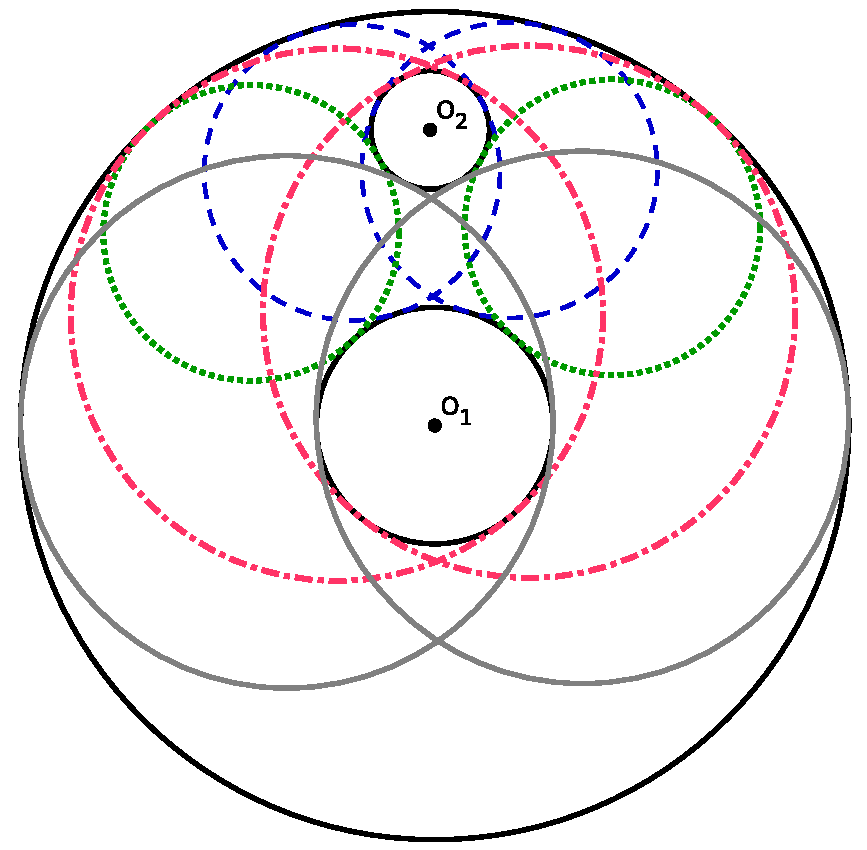
\includegraphics[width=7cm]{../Topicos/Figuras/circunftangentes.pdf} }
 \author{\textbf{Francieli Triches} \\
 \textbf{frantriches@gmail.com} \\ \\ \\
  Esta apostila está licenciada sob uma licença \\
 \href{http://creativecommons.org/licenses/by-sa/4.0/}{Creative Commons Atribuição-Compartilha Igual 4.0 Internacional}.}

\begin{document}
\pagestyle{fancy}

\maketitle

\newpage
\tableofcontents
\listoffigures
%\listoftables

\newpage
 %Este trabalho está licenciado sob a Licença Creative Commons Atribuição-CompartilhaIgual 4.0 Internacional. Para ver uma cópia desta licença, visite https://creativecommons.org/licenses/by-sa/4.0/ ou envie uma carta para Creative Commons, PO Box 1866, Mountain View, CA 94042, USA.

\chapter{Programa do curso}

\begin{small}
\begin{enumerate}
\item Aritmética básica.
\begin{enumerate}[1.1]
\item Álgebra dos números reais: adição, multiplicação e divisão, incluindo operações com frações.
\item Potenciação e radiciação: operações com potências inteiras e racionais.
\item Expressões polinomiais: adição, multiplicação e produtos notáveis.
\item Expressões racionais: adição, multiplicação, divisão de polinômios e racionalização.
\item Resolução de equações lineares.
\item Resolução de equações de segundo grau: fórmula de Bhaskara.
\item Intervalos e valor absoluto.
\item Desigualdades e inequações.
\end{enumerate}

\item Funções reais.
\begin{enumerate}[2.1]
\item Funções reais: definição, domínio e imagem.
\item O plano cartesiano e gráficos de funções reais.
\item Transformações de funções reais e seus gráficos: translação, dilatação e reflexão.
\item Operações com funções reais: adição, multiplicação e composição.
\item Funções injetivas e suas inversas.
\item Funções lineares e seus gráficos.
\item Funções quadráticas e seus gráficos.
\end{enumerate}

\item Funções exponencial e logarítmica e trigonometria.
\begin{enumerate}[3.1]
\item Função exponencial: definição, propriedades e gráfico.
\item Função logarítmica: definição, propriedades e gráfico.
\item Resolução de equações exponenciais e logarítmica.
\item O círculo trigonométrico.
\item Funções seno e cosseno: definição, propriedades e identidades.
\item Outras funções trigonométricas: tangente, cotangente, secante e cossecante.
\item Funções trigonométricas inversas.
\end{enumerate}
\end{enumerate}
\end{small}

 \chapter{Só para garantir!}
 Caso não lembre fique a vontade para colar:
 \section{Tabuada}
 
 \begin{align*} 
 & 1 \times 1= 1 & 2 \times 1= 2 & & 3 \times 1= 3 & & 4 \times 1= 4 & & 5 \times 1= 5 &\\
 & 1 \times 2= 2 & 2 \times 2= 4 & & 3 \times 2= 6 & & 4 \times 2= 8 & & 5 \times 2= 10 &\\
 & 1 \times 3= 3 & 2 \times 3= 6 & & 3 \times 3= 9 & & 4 \times 3= 12 & & 5 \times 3= 15 &\\
 & 1 \times 4= 4 & 2 \times 4= 8 & & 3 \times 4= 12 & & 4 \times 4= 16 & & 5 \times 4= 20 &\\
 & 1 \times 5= 5 & 2 \times 5= 10 & & 3 \times 5= 15 & & 4 \times 5= 20 & & 5 \times 5= 25 &\\
 & 1 \times 6= 6 & 2 \times 6= 12 & & 3 \times 6= 18 & & 4 \times 6= 24 & & 5 \times 6= 30 &\\
 & 1 \times 7= 7 & 2 \times 7= 14 & & 3 \times 7= 21 & & 4 \times 7= 28 & & 5 \times 7= 35 &\\
 & 1 \times 8= 8 & 2 \times 8= 16 & & 3 \times 8= 24 & & 4 \times 8= 32 & & 5 \times 8= 40 &\\
 & 1 \times 9= 9 & 2 \times 9= 18 & & 3 \times 9= 27 & & 4 \times 9= 36 & & 5 \times 9= 45 &\\
 & 1 \times 10= 10 & 2 \times 10= 20 & & 3 \times 10= 30 & & 4 \times 10= 40 & & 5 \times 10= 50 & 
 \end{align*}
 
 \begin{align*} 
 & 6 \times 1= 6 & 7 \times 1= 7 & & 8 \times 1= 8 & & 9 \times 1= 9 & & 10 \times 1= 10 &\\
 & 6 \times 2= 12 & 7 \times 2= 14 & & 8 \times 2= 16 & & 9 \times 2= 18 & & 10 \times 2= 20 &\\
 & 6 \times 3= 18 & 7 \times 3= 21 & & 8 \times 3= 24 & & 9 \times 3= 27 & & 10 \times 3= 30 &\\
 & 6 \times 4= 24 & 7 \times 4= 28 & & 8 \times 4= 32 & & 9 \times 4= 36 & & 10 \times 4= 40 &\\
 & 6 \times 5= 30 & 7 \times 5= 35 & & 8 \times 5= 40 & & 9 \times 5= 45 & & 10 \times 5= 50 &\\
 & 6 \times 6= 36 & 7 \times 6= 42 & & 8 \times 6= 48 & & 9 \times 6= 54 & & 10 \times 6= 60 &\\
 & 6 \times 7= 42 & 7 \times 7= 49 & & 8 \times 7= 56 & & 9 \times 7= 63 & & 10 \times 7= 70 &\\
 & 6 \times 8= 48 & 7 \times 8= 56 & & 8 \times 8= 64 & & 9 \times 8= 72 & & 10 \times 8= 80 &\\
 & 6 \times 9= 54 & 7 \times 9= 63 & & 8 \times 9= 72 & & 9 \times 9= 81 & & 10 \times 9= 90 &\\
 & 6 \times 10= 60 & 7 \times 10= 70 & & 8 \times 10= 80 & & 9 \times 10= 90 & & 10 \times 10= 100 & 
 \end{align*}
 
 \newpage
 \section{Regras de Divisibilidade}
 \begin{itemize}
  \item \textbf{Divisibilidade por $1$}
 
 Todo número é divisível por $1$.
 
 \item \textbf{Divisibilidade por $2$}
 
 Todo número par é divisível por $2$, para isto basta ter unidade igual à $\{0, 2, 4, 6, 8\}$.
 
 \item \textbf{Divisibilidade por $3$}
 
 Um número é divisível por $3$ se a soma de seus algarismos é um número múltiplo de $3$.
 
 \item \textbf{Divisibilidade por $4$}
 
 Um número é divisível por $4$ quando for par e a metade do último algarismo adicionado ao penúltimo for um número par ou terminar com zero nas duas últimas casas.
 
 \item \textbf{Divisibilidade por $5$}
 
 Um número é divisível por $5$ quando terminar em $0$ ou $5$.
 
 \item \textbf{Divisibilidade por $6$}
 
 Um número é divisível por $6$ quando for divisível por $2$ e $3$.
 
 \item \textbf{Divisibilidade por $7$}
 
 Um número é divisível por $7$ quando estabelecida a diferença entre o dobro do último e os demais algarismos, constituindo um número divisível por $7$.
 
 \item \textbf{Divisibilidade por $8$}
 
 Um número é divisível por $8$ quando termina em $000$ ou os últimos três números são divisíveis por $8$.
 
 \item \textbf{Divisibilidade por $9$}
 
 Será divisível por $9$ todo número em que a soma de seus algarismos constitui um número múltiplo de $9$.
 
 \item \textbf{Divisibilidade por $10$}
 
 Um número é divisível por $10$ quando terminar em $0$.
 
 \item \textbf{Divisibilidade por $12$}
 
 Se um número é divisível por $3$ e $4$, também será divisível por $12$.
 
 \item \textbf{Divisibilidade por $15$}
 
 Todo número divisível por $3$ e $5$ também é divisível por $15$.
 \end{itemize}
 
  \newpage
 \section{Símbolos matemáticos}
 
  \begin{table}[H]
 \centering
 \begin{tabular}{|c|c|} \hline
 \rowcolor{cinza}
 Símbolos & Significado \\\hline
 $\forall$ & Para todo \\\hline
 $\exists$ & Existe \\\hline
 $\nexists$ & Não existe \\\hline
 $\in$ & Pertence \\\hline
 $\notin$ & Não pertence \\\hline
 $\infty$ & Infinito \\\hline
 $\emptyset$ & Vazio \\\hline
 $=$ & Igual \\\hline
 $\neq$ & Diferente \\\hline
 $<$ & Menor \\\hline
 $\leq$ & Menor ou igual \\\hline
 $>$ & Maior \\\hline
 $\geq$ & Maior ou igual \\\hline
 $\subset$ & Contido \\\hline
 $\supset$ & Contém \\\hline
 $\subseteq$ & Contido e pode ser igual \\\hline
 $\supseteq$ & Contém e pode ser igual \\\hline
 $\cup$ & União \\\hline
 $\cap$ & Interseção \\\hline
 $\N$ & Números Naturais \\\hline
 $\Z$ & Números Inteiros \\\hline
 $\Q$ & Números Racionais \\\hline
 $\R$ & Números Reais \\\hline
 $\C$ & Números Complexos \\\hline
 
 \end{tabular}
 \end{table}



\chapter{Teoria de conjuntos}

%Texto baseado em Topologia-Elon e \cite{munkres}.

Chamamos de \textbf{conjunto} uma coleção de objetos que satifazem uma propriedade comum. Usaremos letras maiúsculas $A, B, \ldots$ para representar  conjuntos, e letras minúsculas $a, b, \ldots$ para representar seus elementos.

A notação $x \in A$ (lê-se "$x$ pertence à $A$) significa que $x$ é um elemento de $A$. A notação $x \notin A$ (lê-se "$x$ não pertence à $A$) significa que $x$ não é um elemento de $A$.

Dados os elementos $a, e, i, o, u$ indica-se com $\{a, e, i, o, u\}$ o conjunto que é formado por estes elementos. Assim, por exemplo, $V= \{a, e, i, o, u\}$ é o conjunto das vogais do alfabeto português, quando representamos um conjunto desta forma dizemos que estamos representando o conjunto por enumeração de seus elementos.

Assim se denotarmos por $U$ o conjunto formado pelas letras do alfabeto português, como toda vogal é uma letra do alfabeto português, podemos representar o conjunto $V$ da seguinte forma:
\[V= \{x \in U \mid x \text{ é uma vogal}\}\]
aqui $x$ representa um elemento qualquer do conjunto $U$.

Esta segunda forma que usamos para descrever o conjunto $V$ é uma forma usual de descrever conjuntos na matemática, perceba que nela começamos pensando em um conjunto "grande" $U$ (que chamamos de conjunto universo) e em uma propriedade $P$ bem particular que alguns elementos deste conjunto satifaziam, e assim obtemos o conjunto $V$.

Além de relacionar elementos com conjuntos podemos relacionar dois conjuntos, uma forma de relacionar dois conjuntos é através da relação de \textit{inclusão}, que é descrita da seguinte forma, dados dois conjuntos $M$ e $N$, diremos que $M$ está contido em $N$ se todo elemento de $M$ é também um elemento de $N$, neste caso escrevemos $M \subset N$.

Note que em nosso exemplo anterior $V \subset U$, já que toda vogal é também uma letra do alfabeto português. Outro exemplo: como $a$ é um elemento de $V$. Dizer que $a \in V$ é equivalente a afirmar que $\{a\} \subset V$.

\vskip0.4cm

Considerando três conjuntos quaisquer $A$, $B$ e $C$, a relação de inclusão entre eles possui das seguintes propriedades:

\textit{Reflexividade:} para todo conjunto A, tem-se que $A \subset A$.

\textit{Anti-simetria:} se $A \subset B$ e $B \subset A$ então, $A= B$.

\textit{Transitividade:} se $A \subset B$ e $B \subset C$ então, $A \subset C$.

\newpage

Notações:
\begin{itemize}
 \item Elemento $a$ pertence ao conjunto $A$: $\destaque{a \in A}$.
 \item Elemento $a$ não pertence ao conjunto $A$: $\destaque{a \notin A}$.
 \item Conjunto $A$ está contido no conjunto $B$: $\destaque{A \subset B}$.
 \item Conjunto $A$ contém o conjunto $B$: $\destaque{A \supset B}$.
 \item Conjunto $A$ é subconjunto próprio do conjunto $B$: $\destaque{A \varsubsetneq B}$.
 \item O conjunto que não contém nenhum elemento será denotado por $\destaque{\emptyset}= \{ \}$ = conjunto vazio.
\end{itemize}

\vskip0.4cm

 \begin{exem}
  Sejam $A= \{1, 2, 3, 4, 5 \}$ e $B=\{ 2, 3, 4\}$. Então $1 \in A$, mas $1 \notin B$. Além disso, temos que $B \subset A \Rightarrow A \supset B$.
 \end{exem}

 Os conjuntos são também representados através do diagrama de Veen-Euler, no qual basicamente desenhamos um retângulo para representar o conjunto universo, dentro deste retângulo desenhamos um círculo para representar o conjunto, e dentro do círculo escrevemos os elementos que pertencem a este conjunto.

 \begin{exem}
 Consideremos o conjunto das vogais como sendo nosso conjunto universo, assim dentro dele podemos considerar os conjuntos $A= \{a,e, i\}$, e $B=\{a, o, u\}$  estes conjuntos serão representados através do diagrama de Veen-Euler da seguinte forma:

 \begin{center}
  \begin{venndiagram2sets}[labelOnlyA={e i},labelOnlyB={o u},labelAB={a}]
  \end{venndiagram2sets}
  \end{center}


 \end{exem}

 \vskip0.4cm

\section{Operações entre conjuntos}

Dados $A$ e $B$ conjuntos arbitrários dentro do conjunto universo $U$, definimos as seguintes operações entre estes conjuntos:
\begin{itemize}
 \item União:
 $A \cup B=\{x \mid x \in A \text{ ou } x \in B\}.$

 \begin{venndiagram2sets}
  \fillA \fillB
 \end{venndiagram2sets}

 \vskip0.4cm
 \newpage

 \item Interseção:
 $A \cap B=\{x \mid x \in A \text{ e } x \in B\}.$

 \begin{venndiagram2sets}
  \fillACapB
 \end{venndiagram2sets}

 \vskip0.4cm

 \item Diferença:

 $A - B= \{x \mid x \in A \text{ e } x \notin B\}.$

 \begin{venndiagram2sets}
  \fillANotB
 \end{venndiagram2sets}

 $B - A= \{x \mid x \notin A \text{ e } x \in B\}.$

 \begin{venndiagram2sets}
  \fillBNotA
 \end{venndiagram2sets}

 \vskip0.4cm

 \item Complementares:

 $\overline{A}= A^{C}= \{x \in U \mid x \notin A\}$

 \begin{venndiagram2sets}
  \fillNotA
 \end{venndiagram2sets}

 $\overline{B}= B^{C}= \{x \in U \mid x \notin B\}$

 \begin{venndiagram2sets}
  \fillNotB
 \end{venndiagram2sets}

 $\overline{A \cap B}= (A\cap B)^{C}= \{x \in U \mid x \notin (A\cap B)\}$

 \begin{venndiagram2sets}
  \fillNotAorNotB
 \end{venndiagram2sets}

 $\overline{A\cup B}= (A\cup B)^{C}= \{x \in U \mid x \notin (A\cup B)\}$

 \begin{venndiagram2sets}
  \fillNotAorB
 \end{venndiagram2sets}

 \vskip0.4cm

 \item Produto cartesiano:
 $A \times B= \{(a, b) \mid a \in A \text{ e } b \in B \}$

 O produto cartesiano de dois conjuntos pode ser representado usando eixos coordenados, como mostra o exemplo abaixo. Esta representação é particularmente útil para representar os gráficos de funções de $\R$ para $\R$.

 \begin{exem}
  Dados os conjuntos $A= \{1, 2, 3, 4, 5 \}$ e $B=\{ 2, 3, 4, 6\}$, podemos representá-los através do seguinte diagrama de Venn-Euler:
  \begin{center}
  \begin{venndiagram2sets}[labelOnlyA={1 5},labelOnlyB={6},labelAB={2  3  4}]
  \end{venndiagram2sets}
  \end{center}

  Considerando os conjuntos $A$ e $B$ dados, ao aplicar as operações de conjuntos entre eles obtemos os seguintes conjuntos, e suas respectivas representações através do diagrama de Venn-Euler:

  \vskip0.4cm

  $A \cup B=\{ 1, 2, 3, 4, 5 \}$

  \begin{venndiagram2sets}[labelOnlyA={1 5},labelOnlyB={6},labelAB={2  3  4}]
  \fillA \fillB
  \end{venndiagram2sets}

  \vskip0.4cm

  $A \cap B=\{2, 3, 4 \}$

  \begin{venndiagram2sets}[labelOnlyA={1 5},labelOnlyB={6},labelAB={2  3  4}]
  \fillACapB
  \end{venndiagram2sets}

  \vskip0.4cm

  $A - B= \{1, 5 \}$

  \begin{venndiagram2sets}[labelOnlyA={1 5},labelOnlyB={6},labelAB={2  3  4}]
  \fillANotB
  \end{venndiagram2sets}

  \vskip0.4cm

  \begin{eqnarray*}
   A \times B= \{(1, 2), (1, 3), (1, 4), (1, 6), (2, 2), (2, 3), (2, 4), (2, 6), (3, 2), (3, 3), (3, 4), (3, 6), \\
    (4, 2), (4, 3), (4, 4), (4, 6), (5, 2), (5, 3), (5, 4), (5, 6) \}
  \end{eqnarray*}

  \begin{figure}[H]
 \centering
    \fbox{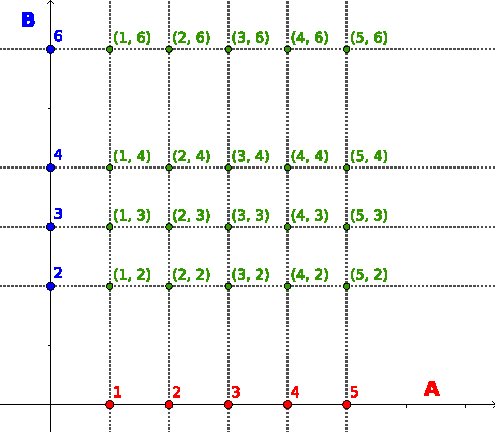
\includegraphics[width=7cm]{../Topicos/Figuras/ProdCartConj.pdf}}
    \caption{Produto cartesiano dos conjuntos $A$ e $B$}
  \end{figure}

 \end{exem}

 \vskip0.4cm

 A \textbf{cardinalidade} de um conjunto $A$ qualquer, é o número de elementos deste conjunto. Denotada por: $n(A)$, $|A|$ ou $\# A$.

 Note que: $n(\emptyset)= \# \emptyset= 0$.

 Dados dois conjuntos $A$ e $B$ quaisquer é importante observar que:
 \vskip0.3cm
 \colorbox{azul}{
 \begin{minipage}{0.9\linewidth}
 \begin{center}
 A cardinalidade da união destes dois conjuntos é dada por:
  \[\#(A \cup B)= \# A + \# B - \#(A \cap B) \ .\]
 \end{center}
 \end{minipage}}
 \vskip0.3cm

 Esta fórmula irá nos ajudar a resolver muitos problemas de teoria de conjuntos.

 \newpage

 Dada uma família $\mathcal{A}$ de conjuntos, ou seja, dado um conjunto $\mathcal{A}$ de conjuntos, temos:
 \item União de todos os conjuntos que são elementos de $\mathcal{A}$:
 $$\bigcup_{A \in \mathcal{A}} A = \{x\mid x \in A \text{ para algum } A \in \mathcal{A}\}$$
 \item Interseção de todos os conjuntos que são elementos de $\mathcal{A}$:
 $$\bigcap_{A \in \mathcal{A}} A = \{x\mid x \in A \text{ para todo } A \in \mathcal{A}\}$$
\end{itemize}

\begin{prop}
Sejam $A$, $B$ e $C$ conjunto arbitrários, temos que:
\begin{itemize}
 \item $\emptyset \subset A$, $\forall A$
 \item $A \cup \emptyset= A$ e $A \cap \emptyset= \emptyset$
 \item $A \cap (B \cup C) = (A \cap B) \cup (A \cap C)$
 \item $A \cup (B \cap C) = (A \cup C) \cap (A \cup C)$
 \item $A - (B \cup C) = (A - B) \cap (A - C)$ (lei de DeMorgan)
 \item $A - (B \cap C) = (A - B) \cup (A - C)$ (lei de DeMorgan)
 \item $\bigcap_{\alpha \in J}(U_{\alpha} \cap Y) = (\bigcap_{\alpha \in J} U_{\alpha}) \cap Y$

  $$(U_1 \cap Y) \cap \cdots \cap (U_n \cap Y) = (U_1 \cap \cdots \cap U_n) \cap Y$$

 \item $\bigcup_{\alpha \in J}(U_{\alpha} \cap Y) = (\bigcup_{\alpha \in J} U_{\alpha}) \cap Y$

 $$(U_1 \cap Y) \cup \cdots \cup (U_n \cap Y) = (U_1 \cup \cdots \cup U_n) \cap Y$$

 \item $(U \times V) \cap (A \times B) = (U \cap A) \times (V \cap B)$

 \item $X - \bigcap_{\alpha \in J} A_{\alpha} = \bigcup_{\alpha \in J}(X - A_{\alpha})$

 \item $X - \bigcup_{i= 1}^{n} A_i = \bigcap_{i = 1}^{n}(X - A_i)$

\end{itemize}
\end{prop}






% \begin{enumerate}[a)]
%  \item
%  \end{enumerate}

%\section{Questões}

 \begin{enumerate}
  \item (FGV - 2017) Manoel cria coelhos e seus animais ou são brancos ou são marrons. Do total dos 120 coelhos que possui, 63 são fêmeas, 50 são marrons e, dos machos, 32 são brancos. O número de fêmeas marrons é:
  \begin{multicols}{5}
  \begin{enumerate}[a)]
  \item 25;
  \item 27;
  \item 29;
  \item 31;
  \item 33.
  \end{enumerate}
  \end{multicols}
  
  \item (IESES - 2017)  Sabendo que temos os conjuntos $A$ e $B$ é \textbf{INCORRETO} afirmar sobre a teoria dos conjuntos que:
  \begin{enumerate}[a)]
  \item A e B são disjuntos quando não possuírem intersecção.
  \item União de A com B é o conjunto formado por elementos que pertencem a A ou B.
  \item Se B é um subconjunto de A, a complementar de A em B é igual a B – A.
  \item Intersecção de A com B é o conjunto dos elementos em comum a A e B.
  \end{enumerate}
  
  \item (CESGRANRIO-2012) Se $P$, $M$ e $N$ são conjuntos e $x$ é tal que $x \notin P \cup M \cup N$ , então:
  \begin{enumerate}[a)]
  \item $x \notin P$  e $x  \notin M$  e $x \notin N$;
  \item $x \notin P$ ou $x \notin M$ ou $x \notin N$;
  \item $x \notin P$ ou $x \notin M \cup N$;
  \item $x \notin P \cap M$ e $x \notin N$;
  \item $x \notin P \cup M$ ou $x \notin N$.
  \end{enumerate}
  
  \item (Quadrix - 2014)  Considere os conjuntos: 
      \[F = \{2, 5, 6, 9,10 \}\]
      \[G = \{3, 4, 7, 8, 12\}\]
 Sabe-se que o conjunto $H$ é formado por uma operação realizada entre os conjuntos $F$ e $G$. Assinale a alternativa que  contém a operação realizada entre os conjuntos $F$ e $G$, que tem como resultado o conjunto $H$, sendo que $H = \varnothing$.
 \begin{enumerate}[a)]
  \item $H= (F \cup G)$;
  \item $H= (F \cap G)$;
  \item $H= (F - G)$;
  \item $H= (G - F)$;
  \item $H= (G \cup F)$.
 \end{enumerate}
 
 \newpage
 \item (FAFIPA - 2014) Sendo os conjuntos $A = \{ x,y,z \}$ e $B =  \{a, x,y,t\}$. Assinale a alternativa que apresenta o conjunto $A - B$:
 \begin{multicols}{5}
 \begin{enumerate}[a)]
  \item $\{ z \}$
  \item $\{ x, y \}$
  \item $\{a, t\}$
  \item  $\{x\}$
 \end{enumerate}
 \end{multicols}
 
 \item (QUADRIX - 2012) Considere os conjuntos: 
  \[ A = \{ x \in \R | - 3 < x < 4 \} \ \ \text{ e } \ \ B = \{ x \in \R | - 2 < x < 5 \}.\]
 O conjunto $B - A$ possui quantos números inteiros?
 \begin{multicols}{5}
 \begin{enumerate}[a)]
  \item 2
  \item 0
  \item 4
  \item 3
  \item 1
 \end{enumerate}
 \end{multicols}
 
 \item (CONSULPLAN - 2014) Sejam os conjuntos $A = \{0, \{1\}, \{2\}, \{3, 4\}\}$ e $B = \{ø, 2, \{3\}, \{0, 3\}\}$. Diante das informações, analise.
 \begin{multicols}{2}
 \begin{enumerate}[I)]
  \item $3 \in B$
  \item $\{3, 4\} \in A$
  \item $\varnothing \nsubset A$
  \item $\varnothing \in B$
 \end{enumerate}
 \end{multicols}
 Estão corretas apenas as alternativas
 \begin{multicols}{2}
 \begin{enumerate}[a)]
 \item I e III.
 \item II e IV.
 \item III e IV.
 \item II, III e IV.
 \end{enumerate}
 \end{multicols}
 
 \item (SOCIESC - Téc. Enfermagem) Dentre as várias opções para compor o prato de almoço do restaurante do Arnaldo, está o feijão e o arroz. De todas as 328 pessoas que almoçaram lá, num determinado período, apenas 20 não optaram por, pelo menos, um dos ingredientes, contra a grande maioria que optou ou em comer somente o arroz, somente o feijão ou, ainda, em misturá-los. Assinale a alternativa que descreve a quantidade total de pessoas que optaram em comer feijão com arroz, se o total de pessoas que NÃO comeram arroz é de 100 pessoas e sabendo que 110 pessoas NÃO comeram feijão.
  \begin{enumerate}
  \item 90
  \item 80
  \item 218
  \item 228
  \item 138
 \end{enumerate}
 
 \newpage
 \item (Lógica - Fundatec - 2018) Em um condomínio de 245 condôminos, sabe-se que 125 usam o salão de jogos, 96 usam o salão de jogos e a piscina. Mas 74 não usam o salão de jogos nem a piscina. Quantos condôminos usam a piscina e não usam o salão de jogos?
\begin{multicols}{5}
\begin{enumerate}[a)]
\item 29
\item 46
\item 75
\item 120
\item 149
\end{enumerate}
\end{multicols}

\item (Lógica - Fundatec - 2018) Todos os funcionários proficientes em espanhol são também proficientes em italiano, mas nenhum funcionário proficiente em italiano é proficiente em francês. Então deduzimos que:
\begin{enumerate}[a)]
\item Algum funcionário é proficiente em espanhol e francês.
\item Todos os funcionários são proficientes em espanhol e francês.
\item Todos os funcionários não são proficientes em francês.
\item Todos os funcionários são proficientes em italiano.
\item Nenhum funcionário é proficiente em francês e espanhol.
\end{enumerate}

\item (Lógica COVEST - UFPE - 2014)  Uma pesquisa entre todos os funcionários de um escritório revelou que: 14 funcionários tomam refrigerante da marca C, 8 tomam refrigerante da marca G, 5 tomam refrigerantes das duas marcas, e 3 não tomam refrigerante. Quantos funcionários tomam precisamente uma marca de refrigerante? 
\begin{enumerate}[a)]
\item 9 
\item 10
\item 11
\item 12
\item 13
\end{enumerate}

 \end{enumerate}
 
 Gabarito:
 1 a); 2 c); 3 a); 4 b); 5 a); 6 e); 7 c); 8 e); 9 b); 10 e); 11 d).
 


\chapter{Conjuntos numéricos}

 \section{Conjunto dos números Naturais (\texorpdfstring{$\N$}{N})}

Os registros mais antigos de números encontrados na história, são de símbolos que eram utilizados para registrar a quantidade de animais, estes símbolos foram sendo aprimorados com o desenvolvimento das sociedades e o aprimoramento da escrita, chegando ao sistema de numeração hindu-arábico que são os números como conhecemos hoje.

Este números que ainda utilizamos para a contagem de objetos são denominados números naturais, como por exemplo:
\[\N= \{0, 1, 2, 3, 4, 5, \ldots \},\]
e o conjunto dos números naturais sem o zero.
\[\N^{*}= \{1, 2, 3, 4, 5, \ldots \}.\]

O zero foi o último deles a ser criado, já que no início não havia necessidade de registro no caso de não se ter posses.
Ainda se discute dentro da matemática se o zero pertence ou não ao conjunto dos números naturais.

É importante notar que neste conjunto numérico temos bem definida apenas a operação de soma/adição (+).

\section{Conjunto dos números Inteiros (\texorpdfstring{$\Z$}{Z})}

Com o surgimento do comércio, surge a necessidade dos comerciantes de registrarem a entrada e saída de bens em seus estabelecimentos, bem como seus lucros e suas despesas. Para efetuar estes registros eles criaram os números negativos, tendo assim como registrar posses usando números positivos e dívidas usando os números negativos.

Este conjunto de números negativos juntamente com os números naturais, forma o conjunto dos números inteiros:
\[\Z= \{ \ldots , -5, -4, -3, -2, -1, 0, 1, 2, 3, 4, 5, \cdots \}\]

Observe que $\N \subset \Z$. E ainda que no conjunto dos números inteiros temos bem definidas as operações de soma (+) e subtração (-).

\section{Conjunto dos números Racionais (\texorpdfstring{$\Q$}{Q})}

Note que no conjunto dos números inteiros ainda não é possível fazer todas as divisões, por exemplo $3 \div 2$ ainda não está definida, pois ainda não existe um número que represente este resultado. Para resolver este problema surge então o conjunto dos números racionais, que é formado por todos os números que podem ser escrito em forma de fração, ou seja o conjunto dos números que podem ser obtidos como resultado de alguma divisão, representamos este conjunto por:
\[\Q= \{ \left(\frac{a}{b}\right) \mid a, b \in \Z \text{ e } b \neq 0 \}.\]

Observe que $\N \subset \Z \subset \Q$. E ainda que no conjunto dos números racionais temos bem definidas as operações de soma (+), subtração (-), multiplicação/vezes (.) e divisão/razão ($\div$). Porém as operações neste conjunto possuem algumas particularidades com as quais devemos ficar atentos, por isso iremos retomá-las na sequência de nossos estudos.

 \vskip0.3cm
 \colorbox{azul}{
 \begin{minipage}{0.9\linewidth}
 \begin{center}
  Chamamos de \textbf{dízimas periódicas} os números decimais com infinitas casas decimais, nos quais a partir de alguma casa decimal, um algarismo ou um grupo de algarismos passa a se repetir infinitamente. O algarismo ou algarismos que se repetem infinitamente constituem o período da dízima.
 \end{center}
 \end{minipage}}
 \vskip0.3cm

 \begin{exem} Vejamos alguns exemplos de dízimas periódicas, e como dada a dízima encontrar a fração que a representa.

  \begin{enumerate}[a)]
   \item Considere o número $0,333 \cdots$, neste caso o período é $3$, assim,
   \[0,3333 \cdots= 0,\overline{3}= \frac{3}{9}= \frac{1}{3}\]
   De fato,
   \begin{eqnarray*}
    x &=& 0,3333 \cdots \\
    10x &=& 10 \cdot 0,3333 \cdots \\
    10x &=& 3,3333 \cdots \\
    10x &=& 3 + 0,3333 \cdots \\
    10x &=& 3 + x \\
    10x - x &=& 3 \\
    9x &=& 3 \\
    x &=& \frac{3}{9} \\
    0,3333 \cdots &=& \frac{1}{3}
   \end{eqnarray*}
   usando a mesma ideia conseguimos mostrar os exemplos abaixo.

   \item Considere o número $0,121212 \cdots$, neste caso o período é $12$, assim,
   \[0,121212 \cdots= 0,\overline{12}= \frac{12}{99}= \frac{4}{33}\]
   \item Considere o número $0,225225225 \cdots$, neste caso o período é $225$, assim,
   \[0,225225225 \cdots= 0,\overline{225}= \frac{225}{999}= \frac{75}{333}=\frac{25}{111}\]
   \item Considere o número $7,464646 \cdots$, neste caso o número tem uma parte inteira que é $7$ e uma parte decimal $0,464646 \cdots$ na qual o período é $46$. Portanto,
   \begin{eqnarray*}
    7,464646 \cdots &=& 7+0,464646 \cdots \\
    &=& 7 + \frac{46}{99} \\
    &=& \frac{7\cdot 99 + 46}{99}\\
    &=& \frac{739}{99}
   \end{eqnarray*}

  \end{enumerate}

 \end{exem}

Concluímos dos exemplos acima que toda dízima periódica é um número racional, assim como os números inteiros, já que, se $a \in \Z$ então $a=\frac{a}{1}$, portanto $a \in \Q$, e os números com um número finito de casas decimais, por exemplo, $0,15= \frac{15}{100}$.


\section{Conjunto dos números Irracionais (\texorpdfstring{$\I$}{I})}

Com o aprimoramento do cálculo de áreas, vem também a necessidade de sabendo a área, por exemplo do quadrado, descobrir quais as medidas de seus lados, dando então origem ao cálculo das raízes quadradas, surge portanto um novo problema, com os números criados até então nem todo número tem uma raiz quadrada. Para resolver este impasse, criou-se o conjunto dos números irracionais, números estes que não podem ser representados por uma fração como por exemplo: $\sqrt{2}$, $\sqrt{3}$, $\sqrt{5}$, $\sqrt{7}$, pi ($\pi$), número de Euler ($e$), e muitos outros. Observe que $\Q \cap \I = \emptyset$.

Números decimais com infinitas casas decimais que não sejam dízimas periódicas são portanto exemplos de números irracionais.

\section{Conjunto dos números Reais (\texorpdfstring{$\R$}{R})}

O mais fácil de definir de todos os conjuntos numéricos apresentados até então é o conjunto dos números reais, onde todas as 4 operações básicas estão bem definidas. O conjunto dos números reais nada mais é do que a união dos números racionais com os números irracionais, $\R= \Q \cup \I$.

Porém como o produto de dois números negativos, é sempre positivo, neste conjunto não podemos calcular a raiz quadrada de qualquer número real, temos portanto mais um problema a ser resolvido, e para tal os matemáticos criaram então mais um conjunto numérico o conjunto dos números complexos!


\section{Conjunto dos números Complexos (\texorpdfstring{$\C$}{C})}

Para resolver o problema da raiz quadrada de um número negativo, criou-se o número imaginário puro $i$, definido por $i= \sqrt{-1}$, portanto $i^2= -1$, criou-se assim um número $i$ que elevado ao quadrado desse $-1$. Temos agora como calcular a raiz quadrada de qualquer número real. Definimos a partir deste número imaginário o conjunto dos números complexos por:
\[\C= \{a + bi; a, b \in \R \} ,\]
cujas operações apresentam algumas particularidades e portanto trataremos delas mais adiante.

Note que, se tivermos $b=0$, estamos com o conjunto dos números reais, portanto $\R \subset \C$. Para fixar a ordem de continência destes conjuntos numéricos, observemos o diagrama de Venn abaixo.

 \begin{figure}[H]
 \centering
    \fbox{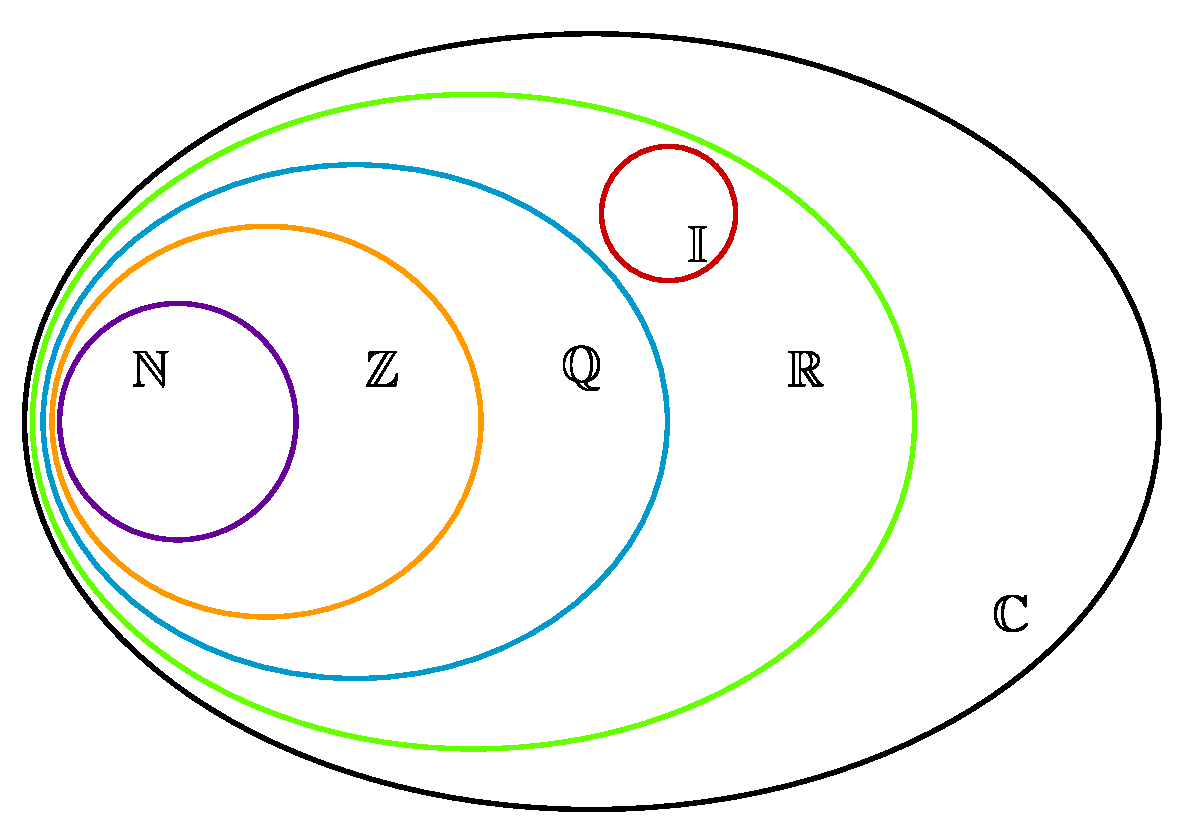
\includegraphics[width=7.5cm]{../Topicos/Figuras/diagrama_conjuntos.pdf}}
    \caption{Representação conjuntos numéricos}
  \end{figure}

\section{Subconjuntos numéricos e suas representações}

\textbf{Intervalos numéricos limitados}
\begin{itemize}
 \item Intervalo aberto: $]a, b[= \{x \in \R \mid a < x < b\}$;
 \begin{figure}[H]
 \centering
 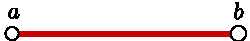
\includegraphics[width=3.5cm]{../Topicos/Figuras/aberto-a-aberto-b.pdf}
 \end{figure}
 \item Intervalo fechado: $[a, b]= \{x \in \R \mid a \leq x \leq b\}$;
 \begin{figure}[H]
 \centering
 
\includegraphics[width=3.5cm]{../Topicos/Figuras/fechado-a-fechado-b.pdf}
 \end{figure}
 \item Intervalo aberto à direita e fechado à esquerda: $[a, b[= \{x \in \R \mid a \leq x < b\}$;
 \begin{figure}[H]
 \centering
 
\includegraphics[width=3.5cm]{../Topicos/Figuras/fechado-a-aberto-b.pdf}
 \end{figure}
 \item Intervalo aberto à esquerda e fechado à direita: $]a, b]= \{x \in \R \mid a < x \leq b\}$.
 \begin{figure}[H]
 \centering
 
\includegraphics[width=3.5cm]{../Topicos/Figuras/aberto-a-fechado-b.pdf}
 \end{figure}
\end{itemize}



\textbf{Intervalos numéricos ilimitados}
\begin{itemize}
\item Conjunto dos números reais maiores que $a$: $[a, +\infty[ = \{ x \in \R \mid a < x \}$
 \begin{figure}[H]
 \centering
 
\includegraphics[width=3.5cm]{../Topicos/Figuras/aberto-a-inf.pdf}
 \end{figure}

\item Conjunto dos números reais maiores ou iguais à $a$: $[a, +\infty[ = \{ x \in \R \mid a \leq x \}$
 \begin{figure}[H]
 \centering
 
\includegraphics[width=3.5cm]{../Topicos/Figuras/fechado-a-inf.pdf}
 \end{figure}

\item Conjunto dos números reais menores que $b$: $]-\infty, b] = \{ x \in \R \mid x < b \}$
 \begin{figure}[H]
 \centering
 
\includegraphics[width=3.5cm]{../Topicos/Figuras/inf-aberto-b.pdf}
 \end{figure}

\item Conjunto dos números reais menores ou iguais à $b$: $]-\infty, b] = \{ x \in \R \mid x \leq b \}$
 \begin{figure}[H]
 \centering
 
\includegraphics[width=3.5cm]{../Topicos/Figuras/inf-fechado-b.pdf}
 \end{figure}

\item Conjunto dos números reais: $]-\infty, +\infty[ = \R$
 \begin{figure}[H]
 \centering
 
\includegraphics[width=7.5cm]{../Topicos/Figuras/reta.pdf}
 \end{figure}
\end{itemize}


\textbf{Outros subconjuntos dos números Reais}
\begin{itemize}
 \item Conjunto dos números reais não-nulos: $\R^{*}=\{x \in \R \mid x \neq 0\}$;
 \begin{figure}[H]
 \centering
 
\includegraphics[width=7.5cm]{../Topicos/Figuras/n-nulos.pdf}
 \end{figure}
 \item Conjunto dos números reais não-negativos: $\R_{+}=\{x \in \R \mid x \geq 0\}$;
 \begin{figure}[H]
 \centering
 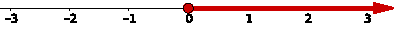
\includegraphics[width=7.5cm]{../Topicos/Figuras/n-negativos.pdf}
 \end{figure}
 \item Conjunto dos números reais positivos: $\R^{*}_{+}=\{x \in \R \mid x > 0\}$;
 \begin{figure}[H]
 \centering
 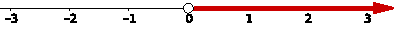
\includegraphics[width=7.5cm]{../Topicos/Figuras/positivos.pdf}
 \end{figure}
 \item Conjunto dos números reais não-positivos: $\R_{-}=\{x \in \R \mid x \leq 0\}$;
 \begin{figure}[H]
 \centering
 
\includegraphics[width=7.5cm]{../Topicos/Figuras/n-positivos.pdf}
 \end{figure}
 \item Conjunto dos números reais negativos: $\R^{*}_{-}=\{x \in \R \mid x < 0\}$.
 \begin{figure}[H]
 \centering
 
\includegraphics[width=7.5cm]{../Topicos/Figuras/negativos.pdf}
 \end{figure}
\end{itemize}

%\section{Questões}
  
  \begin{enumerate}
   \item (FUNDATEC - 2012)  Considerando os seguintes conjuntos:
         \[ A = \{x \in \N | x < 5\}\]
         \[ B = \{x \in \Z | 3x + 4 = 13\}\]
         \[ C = \{x \in \R | x^2 + x – 12 = 0 \} \]
   é correto afirmar que: 
   \begin{enumerate}
   \item $A \cap B = \{ 1,2,3\}$
   \item $A \cup B = B$
   \item $A - B = \{0,1,2,4\}$
   \item $A \cup B \subset C$
   \item $B \cup C= \R$
  \end{enumerate}
  
 \item (TJ/SC - 2018) Três caixas, despachadas pelo correio, tinham os pesos a seguir:
 \begin{table}[H]
 \centering
 \begin{tabular}{|c|c|} \hline
 \rowcolor{cinza}
 Caixas & Pesos (Kg) \\ \hline
 X & 3,4 \\ \hline
 Y & 3,42 \\ \hline
 Z & 3,23 \\ \hline
 \end{tabular}
 \end{table}
 A sequência das caixas em ordem crescente de seus pesos é:
  \begin{enumerate}
  \item Y, Z, X.
  \item X, Y, Z.
  \item X, Z, Y.
  \item Z, Y, X.
  \item Z, X, Y.
 \end{enumerate}
  
  \end{enumerate}

  Gabarito: 1 c), 2 e).


\chapter{Divisibilidade}

 Dados dois números $a, b \in \Z$, com $b \neq 0$ calculamos a divisão de $a$ por $b$ como mostra a figura abaixo:

  \begin{figure}[H]
   \centering
   \fbox{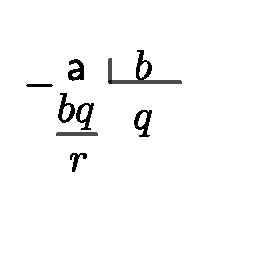
\includegraphics[width=5cm]{../Topicos/Figuras/divisao.pdf}}
   \caption{Representação conjuntos numéricos}
  \end{figure}

 logo, dados $a, b \in \Z$ existem $q, r \in \Z$ tais que $a= bq + r$.

 \vskip0.3cm

 \colorbox{azul}{
 \begin{minipage}{0.9\linewidth}
 \begin{center}
  Um número inteiro $a$ é \textbf{divisível} por um número inteiro $b$, se a divisão de $a$ por $b$ tem resto $r= 0$.
 \end{center}
 \end{minipage}}

 \vskip0.3cm

 \begin{exem}
 \begin{itemize}
 \item Todo número par é divisível por $2$.
 \item Todo número terminado em $0$ ou $5$ é divisível por $5$.
 \item Todo número divisível por $2$ e $3$ é também divisível por $6$.
 \end{itemize}
 \end{exem}

 \vskip0.3cm

 \colorbox{azul}{
 \begin{minipage}{0.9\linewidth}
 \begin{center}
  Um número $a \in \N$ diferente de $0$ e de $1$ é \textbf{primo} se for divisível apenas por $1$ e por ele mesmo.
 \end{center}
 \end{minipage}}


 \begin{exem}
 Primos: $\{2, 3, 5, 7, 11, 13, \ldots \}$
 \end{exem}

 \begin{teo}[Teorema Fundamental da Aritmética]
 Todo número $a \in \N$ diferente de $0$ e de $1$ possui uma decomposição única em números primos, em outras palavras, pode ser escrito como produto de números primos.
 \end{teo}

 \begin{defi}
 Um número $a \in \N$ diferente de $0$ e de $1$ cuja decomposição em primos possui números diferentes de $a$ é chamado de \emph{número composto}. Neste caso, $1$ e $a$ não são os únicos divisores de $a$.
 \end{defi}

 \begin{exem} De números compostos e suas fatorações em números primos:
 \begin{align*}
 &25= 5 \cdot 5 \\
 &12= 2 \cdot 2 \cdot 3 \\
 &15= 3 \cdot 5 \\
 &24= 2 \cdot 2 \cdot 2 \cdot 3
 \end{align*}
 \end{exem}

 Para ilustrar o algoritmo utilizado na fatoração dos números naturais iremos utilizá-lo para fatorar os números acima.

 \begin{tabular}{c|c}
  Números a ser fatorado & Números primos em ordem crescente \\
  25 & 5 \\
  5  & 5 \\
  1  & = 5.5  \\
 \end{tabular}

 \begin{multicols}{3}
   \begin{tabular}{c|c}
  12 & 2 \\
   6 & 2 \\
   3 & 3 \\
   1 & = 2.2.3 \\
 \end{tabular}

 \begin{tabular}{c|c}
  15 & 3 \\
   5 & 5 \\
   1 & = 3.5 \\
 \end{tabular}

 \begin{tabular}{c|c}
  24 & 2 \\
  12 & 2 \\
   6 & 2 \\
   3 & 3 \\
   1 & 2.2.2.3 \\
 \end{tabular}
 \end{multicols}

 \begin{obs}
 Um número natural sempre é divisível por todos os seus fatores primos e também pelos produtos de seus fatores primos.
 \end{obs}

 \begin{exem}
 Como $12= 2 \cdot 2 \cdot 3$, temos que seus divisores são: \[D(12)= \{1, 2, 3, 4, 6, 12\}.\]
 Como $24= 2 \cdot 2 \cdot 2 \cdot 3$, temos que seus divisores são: \[D(24)= \{1, 2, 3, 4, 6, 8, 12, 24\}.\]
 \end{exem}

 \vskip0.3cm
 \colorbox{azul}{
 \begin{minipage}{0.9\linewidth}
 \begin{center}
  \textbf{MDC - máximo divisor comum}

  Dados dois números $a, b \in \N$, o máximo divisor comum entre eles, é o maior número natural que divide $a$ e $b$. Se MDC$(a, b)= 1$ então $a$ e $b$ são primos entre si.
 \end{center}
 \end{minipage}}

 \vskip0.3cm

 \colorbox{azul}{
 \begin{minipage}{0.9\linewidth}
 \begin{center}
 \textbf{MMC - mínimo múltiplo comum}

 Dados dois números $a, b \in \N$, o mínimo múltiplo comum entre eles, é o menor número natural divisível por $a$ e $b$. Se $a$ e $b$ são primos entre si então MMC$(a, b)= ab$.
 \end{center}
 \end{minipage}}


 \begin{exem}
 \begin{align*}
 & \text{MDC}(12, 24)= 12 \\
 & \text{MMC}(12, 24)= 24
 \end{align*}
 \end{exem}

 O cálculo do MMC entre dois números pode ser feito rapidamente com auxílio de seguinte algoritmo, que apresentaremos através de exemplos:

  \begin{exem}
  \begin{enumerate}[a)]
  \item MMC(12, 24):

 \begin{tabular}{c|c}
  12, 24 & 2 \\
   6, 12 & 2 \\
   3,  6 & 2 \\
   3,  3 & 3 \\
   1,  1 &
 \end{tabular}
 $MMC(12, 24) = 2.2.2.3= 24$. Neste caso observe que 24= 2.12.

   \item MMC(9, 10):

   \begin{tabular}{c|c}
    9, 10 & 2 \\
    9, 5  & 3 \\
    3, 5  & 3 \\
    1, 5  & 5 \\
    1, 1  & \\
   \end{tabular}
   $MMC(9, 10)= 2.3.3.5= 90= 9.10$. Neste caso como 9 e 10 não possuem nenhum divisor comum, nesta situação dizemos que eles são primos entre si.

   \item MMC(12, 20):

   \begin{tabular}{c|c}
    12, 20 & 2 \\
     6, 10 & 2 \\
     3,  5 & 3 \\
     1,  5 & 5 \\
     1,  1 & \\
   \end{tabular}
  $MMC(12, 20)= 2.2.3.5= 60 < 12.20= 240$. Este é um caso em que calcular o MMC será uma vantagem, pois o MMC é menor que o produto dos dois números.

  \item MMC(7, 15):

  \begin{tabular}{c|c}
   7, 15 & 3 \\
   7,  5 & 5 \\
   7,  1 & 7 \\
   1,  1 &  \\
  \end{tabular}
  $MMC(7, 15)= 3.5.7= 105$. Observe que neste caso o número 7 é primo, e o número 15 não é um múltiplo de 7, sempre que esta situações ocorrer o MMC entre os números será o produto deles.
  \end{enumerate}

 \end{exem}

%\section{Questões}
 
 \begin{enumerate}
  \item (FEPESE - 2013) Um ônibus está circulando com 40 passageiros e tem 4 paradas pela frente até o destino final. Sabe-se que na primeira parada entram 7 e saem 9 passageiros do ônibus. Ainda, a cada parada subsequente o número de passageiros que entram é o dobro do número de passageiros que entraram na parada anterior e o mesmo vale para o número de passageiros que saem. Logo, ao chegar ao destino final, o número de passageiros no ônibus é de:
 \begin{enumerate}[a)]
 \item 5
 \item 10
 \item 15
 \item 20
 \item 30
 \end{enumerate}

 
 \item (FEPESE - 2013) Uma pessoa deve colocar 312 lâmpadas brancas e 845 lâmpadas amarelas em caixas, de maneira que todas as caixas tenham o mesmo número de lâmpadas, o número de lâmpadas amarelas em cada caixa seja igual e não sobrem lâmpadas fora das caixas. Logo, o número de caixas necessárias para fazer tal divisão é:
  \begin{enumerate}[a)]
  \item 8
  \item 9
  \item 10
  \item 11
  \item 13
  \end{enumerate}

  
  \item (FEPESE - 2016) João trabalha 5 dias e folga 1, enquanto Maria trabalha 3 dias e folga 1. Se João e Maria folgam no mesmo dia, então quantos dias, no mínimo, passarão para que eles folguem no mesmo dia novamente?
  \begin{enumerate}[a)]
  \item 8
  \item 10
  \item 12
  \item 15
  \item 24
  \end{enumerate}

  
  \item (FEPESE - 2016) Em uma excursão participam 120 homens e 160 mulheres. Em determinado momento é preciso dividir os participantes em grupos formados somente por homens ou somente por mulheres, de maneira que os grupos tenham o mesmo número de integrantes. Neste caso, o número máximo de integrantes em um grupo é:
  \begin{enumerate}[a)]
  \item 10
  \item 15
  \item 20
  \item 30
  \item 40
  \end{enumerate}

  
  \item (VUNESP - 2017) Uma papelaria precisa organizar seu estoque de cadernos e, para isso, irá utilizar caixas de papelão, colocando em cada uma delas o mesmo número de cadernos. Se forem colocados 30 cadernos em cada caixa, todas as caixas serão utilizadas e 20 cadernos ficarão de fora, mas, se forem colocados 35 cadernos em cada caixa, todos os cadernos serão encaixotados e 2 caixas não serão utilizadas. Se essa papelaria decidir colocar 40 cadernos em cada caixa, todos os cadernos também serão encaixotados, e o número de caixas necessárias será
  \begin{enumerate}[a)]
  \item 12
  \item 14
  \item 16
  \item 18
  \item 20
  \end{enumerate}

  
   \item (FEPESE - 2013) Em uma fábrica, a entrega do insumo A ocorre a cada 18 dias e do insumo B, a cada 24 dias. Se ambos os insumos são entregues no dia de hoje, em quantos dias ambos serão novamente entregues simultaneamente?
  \begin{enumerate}[a)]
  \item 32
  \item 44
  \item 60
  \item 72
  \item 144
  \end{enumerate}

  
  \item (VUNESP - 2017) Se, numa divisão, o divisor e o quociente são iguais, e o resto é 10, sendo esse resto o maior possível, então o dividendo é
  \begin{enumerate}[a)]
  \item 131
  \item 121
  \item 120
  \item 110
  \item 101
  \end{enumerate}

  
   \item (FGV - 2017) Uma corda de 7 metros e 20 centímetros de comprimento foi dividida em três partes iguais. O comprimento de cada parte é: 
 
  \begin{enumerate}[a)]
  \item 2 metros e 40 centímetros;
  \item 2 metros e 50 centímetros;
  \item 2 metros e 60 centímetros;
  \item 2 metros e 70 centímetros;
  \item 2 metros e 80 centímetros.
  \end{enumerate}
  
 \item (TJ/SC - 2018) Vanda foi ao consultório médico em uma segunda-feira. O médico disse que ela deveria tomar um comprimido de certo remédio todos os dias, durante 180 dias. Vanda começou a tomar o remédio no mesmo dia da consulta e cumpriu exatamente o que disse o médico.
  O primeiro dia que Vanda NÃO precisou tomar o remédio foi:
  \begin{enumerate}
  \item Uma quarta-feira;
  \item Uma quinta-feira;
  \item Uma sexta-feira;
  \item Um sábado;
  \item Um domingo.
 \end{enumerate}
 \end{enumerate}

 Gabarito: 1 b); 2 e); 3 c); 4 e); 5 b); 6 d); 7 d); 8 a); 9 d).
 



 \chapter{Operações Numéricas}

 Antes de tratar das operações numéricas e algébricas, vale ressaltar que quando estamos resolvendo uma expressão numérica ou uma expressão algébrica temos vários cálculos para serem feitos sucessivamente, e para tal precisamos obedecer uma ordem de prioridades que é a seguinte:

\begin{multicols}{2}
Resolva em:
\begin{itemize}
\item 1º lugar: raízes e potências;
\item 2º lugar: multiplicação e divisão;
\item 3º lugar: adição e subtração.
\end{itemize}

Priorize cálculos em:
\begin{itemize}
\item 1º lugar: parênteses $($ $)$;
\item 2º lugar: colchetes $[$ $]$;
\item 3º lugar: chaves $\{$ $\}$.
\end{itemize}
\end{multicols}

 \section{Operações em \texorpdfstring{$\N$}{N}}
 No conjunto dos números naturais, que vamos considerar aqui que contém o $0$ (zero) temos bem definida a operação de soma de dois elementos deste conjunto, pois dados $x$, $y \in \N$ temos que existe $z \in \N$ tal que $x+y=z$, e que $y+x=z$. Por exemplo, $2+3=5=3+2$. \emph{Sugestão ao leitor: pense em outros exemplos numéricos.}
 
 Neste conjunto temos um elemento neutro com relação a operação de soma que é o $0$ (zero), pois dado $x \in \N$, temos que $x+0=x=0+x$.
 
 Mas um fato bem importante com relação a operação de soma em $\N$ é que neste conjunto os elementos não possuem inverso com relação a soma, pois dado $x \in \N$ não existe $y \in \N$ tal que $x+y=0$. Por exemplo, dado $3 \in \N$ não existe $y \in \N$ tal que $3 + y=0$. E ainda a ``operação de subtração'' também não está definida neste conjunto pois, $(4)-(6)=-2$ e $-2 \notin \N$.
 
 No conjunto dos números naturais, temos bem definida também a operação de multiplicação de dois elementos deste conjunto, pois dados $x$, $y \in \N$ temos que existe $z \in \N$ tal que $x \cdot y=z$, e que $y \cdot x=z$. Por exemplo, $2 \cdot 3=6=3 \cdot2$. \emph{Sugestão ao leitor: pense em outros exemplos numéricos.}
 
 Neste conjunto temos um elemento neutro com relação a operação de multiplicação que é o $1$ (um), também chamado de unidade, pois dado $x \in \N$, temos que $x \cdot 1= x= 1 \cdot x$.

 Mas um fato bem importante com relação a operação de multiplicação em $\N$ é que neste conjunto os elementos não possuem inverso com relação a multiplicação, pois dado $x \in \N$ não existe $y \in \N$ tal que $x \cdot y= 1$. Por exemplo, dado $3 \in \N$ não existe $y \in \N$ tal que $3 \cdot y= 1$. Além disso a ``operação de divisão'' também não está definida neste conjunto pois, $(1)\div (2)= 0,5$ e $0,5 \notin \N$. 
 
  \vskip0.3cm
 
 Portanto em $\N$ as operações de soma $(+)$ e multiplicação $(\cdot)$ possuem as seguintes propriedades:
 
 Soma $(+)$:
 \begin{enumerate}[1)]
 \item Fechamento: dados $x, y \in \N$ temos que $x+y \in \N$;
 \item Associativo: dados $x, y, z \in \N$ temos que $(x+y)+z= x+(y+z)$;
 \item Elemento neutro: existe um elemento $0 \in \N$ tal que $x+0=0+x=x$, para qualquer $x \in \N$;
 \item Comutatividade: dados $x, y \in \N$ temos que $x+y= y+x$.
 \end{enumerate}
 
  Multiplicação $(\cdot)$:
 \begin{enumerate}[1)]
 \item Fechamento: dados $x, y \in \N$ temos que $x \cdot y \in \N$;
 \item Associativo: dados $x, y, z \in \N$ temos que $(x \cdot y) \cdot z= x \cdot (y \cdot z)$;
 \item Elemento neutro: existe um elemento $1 \in \N$ tal que $x \cdot 1= 1 \cdot x= x$, para qualquer $x \in \N$;
 \item Comutatividade: dados $x, y \in \N$ temos que $x \cdot y= y \cdot x$.
 \end{enumerate}
 
 Leis distributivas: $\forall x, y, z \in \N$
 \begin{enumerate}[1)]
 \item $x \cdot (y + z)= x \cdot y + x \cdot z$;
 \item $(x + y) \cdot z= x \cdot z + y \cdot z$.
 \end{enumerate}

 \section{Operações em \texorpdfstring{$\Z$}{Z}}

 Ao operar neste conjunto numérico precisamos lidar com os números negativos e para isso precisamos dominar os jogos de sinais envolvidos nestas operações, então vamos ver alguns exemplos de operações neste conjunto para entender como lidar com os números negativos.

   \vskip0.3cm
   
 \textbf{Adição de números inteiros}

 \begin{itemize}
  \item Na adição de números inteiros com o mesmo sinal, some os números e conserve o sinal;
  \item Na adição de números inteiros com sinais diferentes, subtraia os números e conserve o sinal do maior.
 \end{itemize}

  \begin{enumerate}[1)]
   \item $123 + 7= 130$
   \item $123 - 7= 116$
   \item $-123 + 7 = -116$
   \item $-123 - 7 = -130$
 \end{enumerate}
 
  Neste conjunto temos um elemento neutro com relação a operação de soma que é o $0$ (zero), pois dado $x \in \Z$, temos que $x+0=x=0+x$.
 
 Além disso, como no conjunto dos números inteiros temos todos os números negativos, então todo elemento de $\Z$ possui um inverso aditivo, ou seja, $\forall x \in \Z$ existe um elemento $-x \in \Z$ tal que $x + (-x)=0$. Consequentemente, decorre que neste conjunto a ``operação de subtração'' esta bem definida, já que dados $x, y \in \Z$ existe $z \in \Z$ tal que $x - y= x+ (-y)= z$.

   \vskip0.3cm
  
 \textbf{Multiplicação e divisão de números inteiros}

  \begin{itemize}
   \item Na multiplicação e divisão de números inteiros com o mesmo sinal o resultado é sempre positivo.
   \item Na multiplicação e divisão de números inteiros com o sinais diferentes o resultado é sempre negativo.
  \end{itemize}

  \begin{multicols}{2}
  \begin{enumerate}[1)]
   \item $8 \cdot 20= 160$
   \item $8 \cdot (-20)= -160$
   \item $-8 \cdot 20= -160$
   \item $(-8) \cdot (-20)= 160$
   \item $45 \div 5= 9$
   \item $45 \div (-5)= -9$
   \item $(-45) \div 5= -9$
   \item $(-45) \div (-5)= 9$
  \end{enumerate}
  \end{multicols}

 Neste conjunto temos um elemento neutro com relação a operação de multiplicação que é o $1$ (um), também chamado de unidade, pois dado $x \in \Z$, temos que $x \cdot 1= x= 1 \cdot x$.

 Mas um fato bem importante com relação a operação de multiplicação em $\Z$ é que neste conjunto os elementos não possuem inverso com relação a multiplicação, pois dado $x \in \Z$ não existe $y \in \Z$ tal que $x \cdot y= 1$. Por exemplo, dado $3 \in \Z$ não existe $y \in \Z$ tal que $3 \cdot y= 1$. Além disso a ``operação de divisão'' também não está definida neste conjunto pois, $(1)\div (2)= 0,5$ e $0,5 \notin \Z$.
 
   \vskip0.3cm
 
 Portanto em $\Z$ as operações de soma $(+)$ e multiplicação $(\cdot)$ possuem as seguintes propriedades:
 
 Soma $(+)$:
 \begin{enumerate}[1)]
 \item Fechamento: dados $x, y \in \Z$ temos que $x+y \in \Z$;
 \item Associativo: dados $x, y, z \in \Z$ temos que $(x+y)+z= x+(y+z)$;
 \item Elemento neutro: existe um elemento $0 \in \Z$ tal que $x+0=0+x=x$, para qualquer $x \in \Z$;
 \item Elemento inverso: dado $x \in \Z$ qualquer, existe um elemento $-x \in \Z$ tal que $x+(-x)=0$;
 \item Comutatividade: dados $x, y \in \Z$ temos que $x+y= y+x$. 
 \end{enumerate}
 
  Multiplicação $(\cdot)$:
 \begin{enumerate}[1)]
 \item Fechamento: dados $x, y \in \Z$ temos que $x \cdot y \in \Z$;
 \item Associativo: dados $x, y, z \in \Z$ temos que $(x \cdot y) \cdot z= x \cdot (y \cdot z)$;
 \item Elemento neutro: existe um elemento $1 \in \Z$ tal que $x \cdot 1= 1 \cdot x= x$, para qualquer $x \in \Z$;
 \item Comutatividade: dados $x, y \in \Z$ temos que $x \cdot y= y \cdot x$. 
 \end{enumerate}
 
  Leis distributivas: $\forall x, y, z \in \Z$
 \begin{enumerate}[1)]
 \item $x \cdot (y + z)= x \cdot y + x \cdot z$;
 \item $(x + y) \cdot z= x \cdot z + y \cdot z$.
 \end{enumerate}
 
  Como a operação de soma em $\Z$ satisfaz as condições de 1 a 4 acima decorre que $(\Z, +)$ é um grupo aditivo, e por satisfazer a propriedade 5 dizemos que este grupo é abeliano. Como a operação de multiplicação em $\Z$ satisfaz é fechada (1) e associativa (2) e além disso satisfaz as leis distributivas decorre que $\Z$ é um anel. Por valer a comutatividade da multiplicação este anel é comutativo.  


 \section{Operações em \texorpdfstring{$\Q$}{Q}}

 As operações no conjunto dos números Racionais envolvem em particular as operações com frações que possuem algumas particularidades por isso façamos uma rápida retomada destas operações.

 \vskip0.3cm

 \colorbox{azul}{
 \begin{minipage}{0.9\linewidth}
 \begin{center}
  \textbf{Soma:} Dados $x, y, a, b \in \Z$ com $a, b \neq 0$ temos:
 \[\frac{x}{a} + \frac{y}{a}= \frac{x+y}{a} \, \text{ ou}, \ \
  \frac{x}{a} + \frac{y}{b}= \frac{xb + ya}{ab} \]
 \end{center}
 \end{minipage}}

 \vskip0.3cm

 \colorbox{azul}{
 \begin{minipage}{0.9\linewidth}
 \begin{center}
  \textbf{Subtração:} Dados $x, y, a, b \in \Z$ com $a, b \neq 0$ temos:
 \[\frac{x}{a} - \frac{y}{a}= \frac{x-y}{a} \, \text{ ou}, \ \
 \frac{x}{a} - \frac{y}{b}= \frac{xb - ya}{ab} \]
 \end{center}
 \end{minipage}}

 \vskip0.3cm

 \begin{exem}
  \textbf{Soma e subtração de frações com mesmo denominador:}

   Quando os denominadores das frações são iguais, mantemos o denominador e operamos os numeradores.
    \vskip0.3cm
   \[\frac{3}{5} + \frac{1}{5}= \frac{3+1}{5}= \frac{4}{5} .\]
    \vskip0.3cm
   \[\frac{3}{5} - \frac{1}{5}= \frac{3-1}{5}= \frac{2}{5} .\]
 \end{exem}

 \begin{exem}
 \textbf{Soma e subtração de frações com denominadores diferentes:}

   Quando os denominadores das frações são diferentes podemos simplesmente multiplicar os denominadores ou calcular o mínimo múltiplo comum entre eles (MMC), a vantagem da segunda opção é que o MMC é menor ou igual ao produto, como podemos ver no exemplo:
    \vskip0.3cm
   \[\frac{2}{4} + \frac{3}{10}= \frac{10 \cdot 2 + 4 \cdot 3}{4 \cdot 10}= \frac{20 + 12}{40}= \frac{32}{40}= \frac{4}{5} .\]
    \vskip0.3cm
   \[\frac{2}{4} - \frac{3}{10}= \frac{10 \cdot 2 - 4 \cdot 3}{4 \cdot 10}= \frac{20 - 12}{40}= \frac{8}{40}= \frac{1}{5} .\]
    \vskip0.3cm
   Observamos que o $MMC(4, 10)= 20$, assim,
    \vskip0.3cm
   \[\frac{2}{4} + \frac{3}{10}= \frac{5 \cdot 2 + 2 \cdot 3}{20}= \frac{10+6}{20}= \frac{16}{20}=\frac{4}{5} .\]
    \vskip0.3cm
   \[\frac{2}{4} - \frac{3}{10}= \frac{5 \cdot 2 - 2 \cdot 3}{20}= \frac{10 - 6}{20}= \frac{4}{20}=\frac{1}{5} .\]
 \end{exem}


 \vskip0.5cm

 \colorbox{azul}{
 \begin{minipage}{0.9\linewidth}
 \begin{center}
  \textbf{Multiplicação:} Dados $a, b, c, d \in \Z$ com $b, d \neq 0$ temos:
 \[\frac{a}{b} \cdot \frac{c}{d}= \frac{a \cdot c}{b \cdot d} \]
 \end{center}
 \end{minipage}}

 \vskip0.3cm
 \begin{exem}
  \textbf{Multiplicação de fração:} na multiplicação devemos multiplicar numerador por numerador e denominador por denominador.
   \[\frac{2}{3} \cdot \frac{6}{4}= \frac{2 \cdot 6}{3 \cdot 4}= \frac{12}{12}= 1 \]
   \[2 \cdot \frac{5}{3}= \frac{2 \cdot 5}{3}= \frac{10}{3}\]
 \end{exem}

 \vskip0.3cm

 \colorbox{azul}{
 \begin{minipage}{0.9\linewidth}
 \begin{center}
  \textbf{Divisão:} Dados $a, b, c, d \in \Z$ com $b, c, d \neq 0$ temos:
 \[\frac{a}{b} \div \frac{c}{d}= \frac{a}{b} \cdot \frac{d}{c} \]
 \end{center}
 \end{minipage}}

 \vskip0.3cm
 \begin{exem}
  \textbf{Divisão de fração:} na divisão conservamos a primeira fração e multiplicamos pelo inverso da segunda.
   \[\frac{2}{3} \div \frac{1}{6}= \frac{2}{3} \cdot \frac{6}{1}= \frac{2 \cdot 6}{3 \cdot 1}= \frac{12}{3}= 4 \]
   \[\frac{4}{\left(\frac{2}{3}\right)}= \frac{4}{1} \cdot \frac{3}{2}= \frac{12}{2}=6\]
 \end{exem}

 Como visto anteriormente existe uma cópia do conjunto dos números inteiros dentro do conjunto dos números racionais, portanto todas as operações de soma e multiplicação dos números inteiros funcionam da mesma forma no conjunto dos racionais, portanto o jogo de sinais para soma e multiplicação nos racionais são iguais aos jogos de sinais nos inteiros, por isso não iremos detalhar aqui. Mas vale chamar atenção para alguns detalhes do conjunto $\Q$.
 
   Neste conjunto temos um elemento neutro com relação a operação de soma que é o $0$ (zero), pois dado $x \in \Q$, temos que $x+0= x= 0+x$.
 
 Além disso, como no conjunto dos números racionais temos todos os números negativos, então todo elemento de $\Q$ possui um inverso aditivo, ou seja, $\forall x \in \Q$ existe um elemento $-x \in \Q$ tal que $x + (-x)=0$. Consequentemente, decorre que neste conjunto a ``operação de subtração'' esta bem definida, já que dados $x, y \in \Q$ existe $z \in \Q$ tal que $x - y= x+ (-y)= z$.
 
 Neste conjunto temos um elemento neutro com relação a operação de multiplicação que é o $1$ (um), também chamado de unidade, pois dado $x \in \Q$, temos que $x \cdot 1= x= 1 \cdot x$.

 Além disso, com relação a operação de multiplicação em $\Q$, vale obervar que neste conjunto os elementos diferentes de $0$ (zero) possuem inverso com relação a multiplicação, pois dado $x \neq 0 \in \Q$ existe $x^{-1}= \frac{1}{x} \in \Q$ tal que $x \cdot x^{-1}= 1$. Por exemplo, dado $3 \in \Q$ existe $3^{-1}= \frac{1}{3} \in \Q$ tal que $3 \cdot \frac{1}{3}= 1$. Portanto a ``operação de divisão'' está definida neste conjunto.
 
   \vskip0.3cm
 
 Portanto em $\Q$ as operações de soma $(+)$ e multiplicação $(\cdot)$ possuem as seguintes propriedades:
 
 Soma $(+)$:
 \begin{enumerate}[1)]
 \item Fechamento: dados $x, y \in \Q$ temos que $x+y \in \Q$;
 \item Associativo: dados $x, y, z \in \Q$ temos que $(x+y)+z= x+(y+z)$;
 \item Elemento neutro: existe um elemento $0 \in \Q$ tal que $x+0=0+x=x$, para qualquer $x \in \Q$;
 \item Elemento inverso: dado $x \in \Q$ qualquer, existe um elemento $-x \in \Q$ tal que $x+(-x)=0$;
 \item Comutatividade: dados $x, y \in \Q$ temos que $x+y= y+x$. 
 \end{enumerate}
 
  Multiplicação $(\cdot)$:
 \begin{enumerate}[1)]
 \item Fechamento: dados $x, y \in \Q$ temos que $x \cdot y \in \Q$;
 \item Associativo: dados $x, y, z \in \Q$ temos que $(x \cdot y) \cdot z= x \cdot (y \cdot z)$;
 \item Elemento neutro: existe um elemento $1 \in \Q$ tal que $x \cdot 1= 1 \cdot x= x$, para qualquer $x \in \Q$;
 \item Elemento inverso: dado $x \in \Q$ qualquer, existe um elemento $x^{-1} \in \Q$ tal que $x \cdot x^{-1}= 1$;
 \item Comutatividade: dados $x, y \in \Q$ temos que $x \cdot y= y \cdot x$. 
 \end{enumerate}
 
  Leis distributivas: $\forall x, y, z \in \Q$
 \begin{enumerate}[1)]
 \item $x \cdot (y + z)= x \cdot y + x \cdot z$;
 \item $(x + y) \cdot z= x \cdot z + y \cdot z$.
 \end{enumerate}
 
  Como a operação de soma em $\Q$ satisfaz as condições de 1 a 4 acima decorre que $(\Q, +)$ é um grupo aditivo, e por satisfazer a propriedade 5 dizemos que este grupo é abeliano. Analogamente, como a operação de multiplicação em $\Q$ satisfaz as propriedades de 1 a 4 decorre que $(\Q, \cdot)$ é um grupo multiplicativo, e por satisfazer a propriedade 5 é um grupo abeliano. Além disso, como a operação de multiplicação em $\Q$ é fechada (1) e associativa (2) e além disso satisfaz as leis distributivas decorre que $\Q$ é um anel. 
  
  Além disso, $\Q$ com as operações de soma e multiplicação, como definidas é também um corpo. Vale aqui observar que todo conjunto com duas operações, soma e multiplicação, bem definidas, satisfazendo as propriedade de 1 a 5 respectivamente, e as leis de distributividade são denominados \emph{corpos}. 
 
 \section{Operações em \texorpdfstring{$\I$}{I} e \texorpdfstring{$\R$}{R}}
 
 Para finalizar, lembramos que há uma cópia dos números racionais dentro do conjunto dos números reais, portanto todas as propriedades das operações em $\Q$ continuam válidas para estes números dentro de $\R$. Assim, para compreendermos como funcionam as operações em $\R= \Q \cup \I$ precisamos aprender a operar em $\I$. As operações entre números irracionais que são raízes de alguma ordem de outros números serão discutidas no próximo capítulo, as operações entre números irracionais como por exemplo $\pi + e$, costumamos deixar indicadas, por este motivo não precisamos detalhar este caso.
 
 Mas destacamos que em $\R$ as operações de soma (adição) $(+)$ e multiplicação $(\cdot)$ possuem as seguintes propriedades:
 
 Soma (adição) $(+)$:
 \begin{enumerate}[1)]
 \item Fechamento: dados $x, y \in \R$ temos que $x+y \in \R$;
 \item Associativo: dados $x, y, z \in \R$ temos que $(x+y)+z= x+(y+z)$;
 \item Elemento neutro: existe um elemento $0 \in \R$ tal que $x+0=0+x=x$, para qualquer $x \in \R$;
 \item Elemento inverso: dado $x \in \R$ qualquer, existe um elemento $-x \in \Q$ tal que $x+(-x)=0$;
 \item Comutatividade: dados $x, y \in \R$ temos que $x+y= y+x$. 
 \end{enumerate}
 
  Multiplicação $(\cdot)$:
 \begin{enumerate}[1)]
 \item Fechamento: dados $x, y \in \R$ temos que $x \cdot y \in \R$;
 \item Associativo: dados $x, y, z \in \R$ temos que $(x \cdot y) \cdot z= x \cdot (y \cdot z)$;
 \item Elemento neutro: existe um elemento $1 \in \R$ tal que $x \cdot 1= 1 \cdot x= x$, para qualquer $x \in \R$;
 \item Elemento inverso: dado $x \in \R$ qualquer, existe um elemento $x^{-1} \in \R$ tal que $x \cdot x^{-1}= 1$;
 \item Comutatividade: dados $x, y \in \R$ temos que $x \cdot y= y \cdot x$. 
 \end{enumerate}
 
  Leis distributivas: $\forall x, y, z \in \R$
 \begin{enumerate}[1)]
 \item $x \cdot (y + z)= x \cdot y + x \cdot z$;
 \item $(x + y) \cdot z= x \cdot z + y \cdot z$.
 \end{enumerate}
 
   Quando um conjunto tem duas operações satisfazendo as propriedades acima ele costuma ser chamado de \emph{corpo}. Portanto, $\R$ é um \emph{corpo}. Este e outros corpos são utilizados em disciplinas como Álgebra Linear.
   
   Só por curiosidade, um outro exemplo de corpo é o conjunto $\Z_2= \{0, 1\}$, no qual definimos $1+1=0$, pois neste conjunto as operações de adição e multiplicação satisfazem todas as propriedades mencionadas anteriormente.

 \chapter{Potenciação}

 \section{Potência com expoente inteiro}

 \vskip0.3cm

 \colorbox{azul}{
 \begin{minipage}{0.9\linewidth}
 \begin{center}
  Dados dois números $a \in \R$ e $b \in \N$ definimos:
 \[a^b= \underbrace{a \cdot a \cdot \cdots \cdot a}_{b \text{ vezes}} .\]
  Dizemos que $a$ é a base da potência e $b$ o expoente. Lê-se: $a$ elevado a $b$.
 \end{center}
 \end{minipage}}

 \vskip0.3cm

 \begin{exem}
 Observe que neste caso o expoente é um número natural, e portanto positivo, como por exemplo:

  $2^3= 2 \cdot 2 \cdot 2= 8$;

  $2^4=2 \cdot 2 \cdot 2 \cdot  2= 16$;

  $3^2= 3 \cdot 3= 9$;

  $5^3= 5 \cdot 5 \cdot 5= 125$.

  Este é o único caso em que temos a potência definida, se tivermos qualquer outro número no expoente precisamos fazer recair nesta situação.
 \end{exem}


 \vskip0.3cm

 \colorbox{azul}{
 \begin{minipage}{0.9\linewidth}
 \begin{center}
   Dados dois números $a \in \R$ e $b \in \Z$ definimos:
 \[a^b= \underbrace{a \cdot a \cdot \cdots \cdot a}_{b \text{ vezes}}, \text{ para } b\geq0, \text{ esta situação está inclusa no caso anterior};\]
 \[a^{-b}= \frac{1}{a^b}= \underbrace{\frac{1}{a} \cdot \frac{1}{a} \cdot \cdots \cdot \frac{1}{a}}_{b \text{ vezes}}, \text{ para } b>0 ;\]
 \[\frac{1}{a^{-b}}= a^b, \text{ para } b>0;\]
 \end{center}
 \end{minipage}}

 \vskip0.3cm

 \begin{exem}
 Vejamos agora alguns exemplos em que o expoente é um número negativo:
 \begin{eqnarray*}
  2^{-1}= \frac{1}{2^{1}}= \frac{1}{2}; \\
  2^{-3}= \frac{1}{2^3}= \frac{1}{8}; \\
  \frac{1}{3^{-2}}= 3^2= 3 \cdot 3= 9; \\
  \left( \frac{8}{22} \right)^{-2}= \left( \frac{22}{8} \right)^{2}= \frac{22}{8} \cdot \frac{22}{8}= \frac{484}{64}.
 \end{eqnarray*}
 Note que em todos os exemplos acima o que fizemos foi ``inverter'' a fração, e com isso deixamos os expoentes positivos, e então basta aplicar a definição de potência.

 \end{exem}

 
 Se $a, b \in \R$, $m, n \in \N$, então valem as seguintes propriedades:
 \begin{enumerate}[P1)]
 \item $a^m \cdot a^n= a^{m + n}$;
 \item $a^m \div a^n= a^{m - n}$, para $a \neq 0$;
 \item $(a^m)^n= a^{m \cdot n}$;
 \item $(a \cdot b)^n= a^n \cdot b^n$;
 \item $\left(\frac{a}{b}\right)^n= \frac{a^n}{b^n}$, para $b \neq 0$;
 \item $a^{-n}= \frac{1}{a^n}$, para $(a \neq 0)$;
 \item $\left(\frac{a}{b} \right)^{-n}= \left(\frac{b}{a} \right)^{n}$, para $a \neq 0$ e $b \neq 0$;
 \end{enumerate}
 
  \vskip0.3cm

 \colorbox{amarelo}{
 \begin{minipage}{0.9\linewidth}
 \begin{center}
 Aqui é importante observar que:
 \begin{align*}
 & \nexists 0^0 & & a^1= a, \forall a \in \R & & a^0= 1, \forall a \in \R & & 1^a= 1, \forall a \in \R
 \end{align*}
 \end{center}
 \end{minipage}}
 
\vskip0.3cm 

 \section{Raiz}
 
 Dados um número real $a \geq 0$ e um número natural $n$, existe um número real positivo ou nulo $b$ tal que $b^n= a$. O número real $b$ é chamado de raiz enézima de $a$, ou raiz de ordem $n$ de $a$ e indicaremos por $\sqrt[n]{a}$.
 
 \begin{obs}
 Da definição decorre que $(\sqrt[n]{a})^n=a$.
 \end{obs}
 
 \begin{obs}
 Note que de acordo com a definição dada $\sqrt{36}= 6$ e não $\sqrt{36}= \pm 6$.
 \end{obs}
 
 \begin{obs}
 Muita atenção ao calcular a raiz quadrada de um quadrado perfeito:
 \[\sqrt{a^2}= |a| \ . \]
 \end{obs}
 
 Se $a, b \in \R_{+}$, $m \in \Z$, $n \in \N^{*}$, e $p \in \N^{*}$, então valem as seguintes propriedades:
 \begin{enumerate}[R1)]
 \item $\sqrt[n]{a^m}= \sqrt[n \cdot p]{a^{m\cdot p}}$;
 \item $\sqrt[n]{a \cdot b}= \sqrt[n]{a} \cdot \sqrt[n]{b}$;
 \item $\sqrt[n]{\frac{a}{b}}= \frac{\sqrt[n]{a}}{\sqrt[n]{b}}$, para $b \neq 0$;
 \item $(\sqrt[n]{a})^m= \sqrt[n]{a^m}$;
 \item $\sqrt[p]{\sqrt[n]{a}}= \sqrt[p \cdot n]{a}$.
 \end{enumerate}

 \section{Potência com expoente racional}
 
 A radiciação pode ser entendida como uma potência com expoente racional, a partir da seguinte definição.
 \vskip0.3cm

 \colorbox{azul}{
 \begin{minipage}{0.9\linewidth}
 \begin{center}
  Dados dois números $a \in \R^{*}_{+}$ e $\frac{m}{n} \in \Q$ ($m \in \Z$ e $n \in N^{*}$), definimos:
 \[a^{\frac{m}{n}}= \sqrt[n]{a^m}, \text{ para } \frac{m}{n} >0 ;\]
 \[a^{-\frac{m}{n}}= \frac{1}{a^{\frac{m}{n}}}= \frac{1}{\sqrt[n]{a^m}},  \text{ para } \frac{m}{n} >0.\]
 \end{center}
 \end{minipage}}

 \vskip0.3cm
 
 Entendida a radiciação como potência são válidas aqui todas as propriedades de potência com expoente inteiro listadas anteriormente.

 \begin{exem}
  Vejamos agora alguns exemplos de potência com expoente sendo um número racional ($b \in \mathbb{Q}$):
  \begin{eqnarray*}
   4^{\frac{1}{2}}= \sqrt{4}= 2 \\
   8^{\frac{1}{3}}= \sqrt[3]{8^1}= \sqrt[3]{2^{3}}= 2 \\
   27^{\frac{2}{6}}= \sqrt[6]{27^2}= \sqrt[6]{729}= \sqrt[6]{3^6}= 3\\
   9^{-\frac{1}{2}}= \frac{1}{9^{\frac{1}{2}}}= \frac{1}{\sqrt{9}}= \frac{1}{3} \\
   \left(\frac{4}{9}\right)^{-\frac{1}{2}}= \left(\frac{9}{4}\right)^{\frac{1}{2}}= \sqrt{\left(\frac{9}{4}\right)}=\frac{\sqrt{9}}{\sqrt{4}}= \frac{3}{2} \\
   \frac{2}{3^{-2}}= 2 \cdot \frac{1}{3^{-2}}= 2 \cdot 3^{2}= 2 \cdot 9= 18
  \end{eqnarray*}

 \end{exem}
 
 \section{Potência com expoente irracional}
 
 Dados um número real $a > 0$ e um número irracional $\alpha$, podemos construir por meio de aproximações sucessivas de potências de $a$ com expoente racional, um único número real positivo $a^{\alpha}$ que é potência de base $a$ e expoente irracional $\alpha$.
 
 Esse método é decorre do fato que um número irracional pode ser aproximado por falta ou por excesso por sequências de números racionais, e potências com expoentes racionais estão bem definidas, então podemos utilizar estes dois fatos e definir potências com expoente irracionais que satifazem todas as propriedades de potências já descritas. Vejamos um exemplo:
 
 \begin{exem}
 Consideremos o número irracional $\sqrt{2}= 1,414213562\ldots$. Observe que podemos aproximar $\sqrt{2}$ por falta ou por excesso pelos seguintes números racionais:
 
 \begin{multicols}{2}
 por falta:
 \begin{eqnarray*}
 1 &=& 1\\
 1,4 &=& \dfrac{14}{10} \\
 1,41 &=& \dfrac{141}{100} \\
 1,414 &=& \dfrac{1414}{1000} \\
 1,4142 &=& \dfrac{14142}{1000}
 \end{eqnarray*}
 
 por excesso:
 \begin{eqnarray*}
 2 &=& 2\\
 1,5 &=& \dfrac{15}{10} \\
 1,42 &=& \dfrac{142}{100} \\
 1,415 &=& \dfrac{1415}{1000} \\
 1,4143 &=& \dfrac{14143}{1000}
 \end{eqnarray*}
 \end{multicols} 
 
 Assim podemos definir o valor de $13^{\sqrt{2}}$ por aproximação por falta ou por excesso de potências de base $13$, da seguinte forma:
 
 por falta:
 \begin{eqnarray*}
 13^1 =& 13^1 &= 13\\
 13^{1,4} =& 13^{\frac{14}{10}} =& 36,267756667 \\
 13^{1,41} =& 13^{\frac{141}{100}} =& 37,210039132 \\
 13^{1,414} =& 13^{\frac{1414}{1000}} =& 37,59377174 \\
 13^{1,4142} =& 13^{\frac{14142}{1000}} =& 37,613061911
 \end{eqnarray*}
 
 por excesso:
 \begin{eqnarray*}
 13^{2} =& 13^{2} =& 169 \\
 13^{1,5} =& 13^{\frac{15}{10}} =& 46,872166581 \\
 13^{1,42} =& 13^{\frac{142}{100}} =& 38,176803296\\
 13^{1,415} =& 13^{\frac{1415}{1000}} =& 37,69032163 \\
 13^{1,4143} =& 13^{\frac{14143}{10000}} =& 37,622710708
 \end{eqnarray*}
 
 Portanto $13^{\sqrt{2}} \approx 37,6$.
 \end{exem}

 Se $a=0$ e $\alpha$ é irracional e positivo, definimos $0^{\alpha}=0$.
 
 \begin{obs}
 Se $a=1$ então $1^{\alpha}= 1, \forall \alpha$ irracional.
 \end{obs}
 
 \begin{obs}
 Se $a < 0$ e $\alpha$ é irracional e positivo então o símbolo $a^{\alpha}$ não tem significado.
 \end{obs}
 
 \begin{obs}
 Se $\alpha$ é irracional e negativo $(\alpha < 0)$ então $0^{\alpha}$ não tem significado.
 \end{obs}
 
 \begin{obs}
 Para as potências de expoente irracional são válidas as propriedades de potências com expoente racional.
 \end{obs}

 \section{Potência com expoente real}
 
 Considerando que já foram definidas anteriormente as potências de base $a \in \R^{*}_{+}$ e expoente $b$ ($b$ racional ou  irracional) então já está definida a potência $a^b$ com $a \in \R^{*}_{+}$ e $b \in \R$.
 
 \begin{obs}
 Toda potência de base real e positiva e expoente real é um número real positivo.
 \[a> 0 \Rightarrow a^b > 0 \ .\]
 \end{obs}
 
  Se $a, b \in \R^{*}_{+}$, $m, n \in \R$, então valem as seguintes propriedades:
 \begin{enumerate}[P1)]
 \item $a^m \cdot a^n= a^{m + n}$;
 \item $a^m \div a^n= a^{m - n}$, para $a \neq 0$;
 \item $(a^m)^n= a^{m \cdot n}$;
 \item $(a \cdot b)^n= a^n \cdot b^n$;
 \item $\left(\frac{a}{b}\right)^n= \frac{a^n}{b^n}$, para $b \neq 0$;
 \item $a^{-n}= \frac{1}{a^n}$, para $(a \neq 0)$;
 \item $\left(\frac{a}{b} \right)^{-n}= \left(\frac{b}{a} \right)^{n}$, para $a \neq 0$ e $b \neq 0$;
 \end{enumerate}
 


 \chapter{Operações Algébricas}

 Expressões algébricas são expressões matemáticas que envolvem números, letras e operações.

 Como por exemplo:

 \begin{eqnarray*}
  2x=4,\\
  x^2+1=0,\\
  x(x+3)=5,\\
  2x+3y=17,\\
  x^2 + 2y + 3z -4= 52, \\
  \frac{14x + 8y}{2x}= 3, \\
  \frac{2}{5}x^3 + 3\sqrt{x^4}= 67, \\
  5x(x+3)-4x(2-x)=7.
 \end{eqnarray*}

 Nestas expressões as letras que aparecem são chamadas de \textbf{variáveis}, e os números que aparecem multiplicando uma letra são chamados de \textbf{coeficientes}.

 As expressões algébricas são utilizadas dentre outras coisas, para descrever uma situação problema na qual não conhecemos todos os valores envolvidos, representar uma fórmula, ou expressar uma equação. Devido a sua importância nas exatas precisamos compreender como se comportam as operações presentes nas expressões algébricas, em outras palavras, como fazer contas com letras.

 \vskip0.3cm

 \textbf{Adição e subtração}

 Podemos somar somente letras iguais e com mesmo expoente. Como por exemplo:

 \begin{itemize}
  \item $2x + x= (2+1)x= 3x$
  \item $x^2 - 3x^2= (1-3)x^2= -2x^2$
  \item $2x + y + 5x^2 + 7y - 3x= 5x^2 + (2-3)x + (1+7)y= 5x^2 - 1x + 8y$
  \item $3(x+ 4y-2)= 3x + 3.4y - 3.2= 3x + 12y - 6$
 \end{itemize}

  \vskip0.3cm

 \textbf{Multiplicação}

 Na multiplicação devemos sempre multiplicar coeficiente por coeficiente e letra por letra. Sendo que no caso das letras serem iguais, devemos manter a letra e somar seus expoentes, e no caso das letras serem diferentes apenas fazemos a associação das duas letras. Como mostram os seguintes exemplos:

  \begin{itemize}
   \item $x \cdot x = x^{1+1}= x^2$
   \item $x \cdot x^2= x^{1+2}= x^3$
   \item $x \cdot 2y= (1 \cdot 2)xy= 2xy$
   \item $3x \cdot 2x^2y= (3 \cdot 2)x^{1+2}y= 6x^3y$
   \item $4x^4 \cdot \frac{1}{2}x^{-2}= (4 \cdot \frac{1}{2})x^{4-2}= 2x^2$
   \item $(x - 1) \cdot (x - 2)= x(x-2) - 1(x-2)= x^2 -2x -x +2= x^2 - 3x + 2$
  \end{itemize}

  \vskip0.3cm

   \textbf{Divisão}

   Na divisão devemos sempre dividir coeficiente por coeficiente e letra por letra. Sendo que no caso das letras serem iguais, devemos manter a letra e subtrair seus expoentes, e no caso das letras serem diferentes apenas fazemos a associação das duas letras. Como mostram os seguintes exemplos:

  \begin{itemize}
   \item $x \div x= x^{1-1}= x^0= 1$
   \item $x \div x^2= x^{1-2}= x^{-1}= \frac{1}{x}$
   \item $2y \div x= 2\frac{y}{x}$
   \item $4y^3 \div 2y^2= \frac{4}{2} \cdot \frac{y^3}{y^2}= 2y^{3-2}= 2y$
   \item $\frac{x^2yz^3}{x^2y^3z^2}= x^{2-2}y^{1-3}z^{3-2}= x^0 y^{-2}z^{1}= \frac{z}{y^2}$
   \item $\frac{(x+3) \cdot (x-1)}{(x-1)\cdot (2x+3)}= \frac{x+3}{2x+3}$
  \end{itemize}

 \vskip0.3cm

  \textbf{Potenciação}

  Na potenciação devemos aplicar o expoente ao coeficiente e à incógnita, obedecendo as propriedades de potência.

    \begin{itemize}
     \item $(2x)^2= 2^2 \cdot x^2= 4x^2$
     \item $(3x^2)^3= 3^3 \cdot x^{2\cdot 3}= 27x^6$
     \item $\left(\frac{3a^2}{4}\right)^2= \frac{3^2 a^{2 \cdot 2}}{4^2}= \frac{9a^4}{16}$
    \end{itemize}

  \vskip0.3cm

  \textbf{Radiciação}

  Na radiciação devemos extrair a raiz do coeficiente e da incógnita. Observamos que extrair a raiz da incógnita é equivalente a dividir seu expoente pelo índice da raiz.
    \begin{itemize}
     \item $\sqrt{x}= x^{\frac{1}{2}}$
     \item $\sqrt{x^4}= (x^4)^{\frac{1}{2}}= x^{\frac{4}{2}}= x^2$
     \item $\sqrt[3]{8x^6}= \sqrt[3]{8} \cdot \sqrt[3]{x^6}= 2 x^{\frac{6}{3}}= 2x^2$
     \item $\sqrt{\frac{2x^2}{16}}= \frac{\sqrt{2x^2}}{\sqrt{16}}= \frac{|x|\sqrt{2}}{4}$
     \item $\sqrt{x^2}= |x|$
    \end{itemize}

 \vskip0.3cm

  \textbf{Fatoração das expressões algébricas}

 \vskip0.3cm

 A fatoração das expressões algébricas, é o que nos permite escrever a expressão como um produto de dois termos, ela é utilizada principalmente na resolução de equações, para acelerar o processo de resolução.

 Os seguintes casos de fatoração são os mais utilizados:
 \begin{itemize}
  \item Fator em comum: $x^2 + x= x(x + 1)$; $4x^2 + 6= 2(2x^2 + 3)$
  \item Agrupamento: $ax + bx + ay + by= (a+b)x+(a+b)y= (a+b)(x+y)$
  \item Trinômio quadrado perfeito (+): $(a + b)^2= a^2 + 2ab + b^2$
  \item Trinômio quadrado perfeito (-): $(a - b)^2= a^2 - 2ab + b^2$
  \item Diferença de dois quadrados: $(a + b) \cdot (a - b)= a^2 - b^2$
  \item Cubo perfeito (+): $(a+b)^3= a^3 + 3a^2b + 3ab^2 + b^3$
  \item Cubo perfeito (-): $(a-b)^3= a^3 - 3a^2b + 3ab^2 - b^3$
 \end{itemize}
 
 \newpage
 \section{Polinômios}
 
  \vskip0.3cm
 \colorbox{azul}{
 \begin{minipage}{0.9\linewidth}
 \begin{center}
  Seja $K= \R \text{ ou } \C$. Um polinômio $p$ na incógnita $x$ e com coeficientes em $K$ (simbolicamente, $p \in K[x]$) é uma expressão da forma
  \[p(x)= a_nx^n + a_{n-1}x^{n-1}+ \ldots + a_1x+ a_0= \sum_{i=0}^{n} a_ix^i ,\]
  em que os coeficientes $a_n, \ldots, a_0 \in K$, $a_n \neq 0$ e $n \in \N$. O número natural $n$ é chamado de grau do polinômio $p$, e escreve-se $gr(p)= n$. O termo $a_0$ é denominado termo constante de $p$.
 \end{center}
 \end{minipage}}
 \vskip0.3cm
 
 \begin{obs}
 Os termos polinômio e função polinomial serão considerados como sinônimos e utilizados sem distinção no decorrer deste texto.
 \end{obs}
 
 Uma função polinomial de grau $0$ é uma função constante; uma função polinomial de grau $1$ é uma função linear (ou, função afim); uma função polinomial de grau $2$ é uma função quadrática.
 
 Por simplicidade, a partir de agora iremos considerar nossos polinômios sobre $\R$, porém esta teoria pode ser estendida sem muita dificuldade para o corpo dos números complexos.
 
 \begin{defi}
 Dados um número real $k$ e o polinômio $p(x)= a_nx^n + a_{n-1}x^{n-1}+ \ldots + a_1x+ a_0$, chama-se \emph{valor numérico de $p$ em $k$} ao valor:
 \[p(k)= a_nk^n + a_{n-1}k^{n-1}+ \ldots + a_1k+ a_0 \ .\]
 \end{defi}
 
\begin{exem}
Por exemplo, se considerarmos o polinômio $p(x)= x^2 + 7x+10$, temos os seguintes valores numéricos para $p$:
\begin{eqnarray*}
p(-6)&=& (-6)^2 + 7(-6) +10= 4\\
p(-5)&=& (-5)^2 + 7(-5) +10= 0\\
p(-4)&=& (-4)^2 + 7(-4) +10= -2\\
p(-2)&=& (-2)^2 + 7(-2) +10= 0\\
p(0)&=& 0^2 + 7 \cdot 0 +10= 10\\
\end{eqnarray*}
\end{exem} 
 
 \begin{defi}
 Em particular, se $k$ é um número real tal que $p(k)= 0$, dizemos que $k$ é uma \emph{raiz} ou \emph{um zero} de $p$.
 \end{defi}
 
 \begin{exem}
 Portanto no exemplo anterior temos que $k_1= -5$ e $k_2=-2$ são raízes do polinômio $p(x)= x^2 + 7x+10$.
 \end{exem}
 
  \begin{defi}
  O polinômio nulo (ou identicamente nulo) é um polinômio da forma $p(x)= 0x^n +0x^{n-1}+ \ldots + 0x+ 0$, ou simplesmente, $p(x)= 0$. Por convenção, o grau deste polinômio será indefinido.
 \end{defi}
 
 
  \begin{teo}
  Sejam $p$ e $q$ dois polinômios em $K$, dados por:
  \[p(x)= a_nx^n + a_{n-1}x^{n-1}+ \ldots + a_1x+ a_0= \sum_{i=0}^{n} a_ix^i\]
  \[q(x)= b_nx^n + b_{n-1}x^{n-1}+ \ldots + b_1x+ b_0= \sum_{i=0}^{n} b_ix^i\]
  temos que $p=q \Leftrightarrow a_i= b_i$, para todo $i \in \{0, 1, 2, \cdots, n\}$.
 \end{teo}
 
 \begin{dem}
 Para todo $x \in \R$, temos:
 \[a_i= b_i \Leftrightarrow a_i - b_i=0 \Leftrightarrow (a_i - b_i)x^i=0 \Leftrightarrow \sum_{i=0}^{n}(a_i - b_i)x^i= 0 \Leftrightarrow\]
 \[ \sum_{i=0}^{n}a_i x^i - \sum_{i=0}^{n}b_i x^i = 0 \Leftrightarrow \sum_{i=0}^{n}a_i x^i = \sum_{i=0}^{n}b_i x^i \Leftrightarrow p(x)= q(x)\]

 \end{dem}
 
  Este Teorema mostra que, quando escrevemos um polinômio $p$ na forma 
 \[p(x)= a_nx^n + a_{n-1}x^{n-1}+ \ldots + a_1x+ a_0\]
 com $a_i \in K$, então os números $a_0, \ldots, a_n$ são determinados de modo único. 
 
 Dados dois polinômios 
 \[p(x)= a_nx^n + a_{n-1}x^{n-1}+ \ldots + a_1x+ a_0= \sum_{i=0}^{n} a_ix^i\]
  \[q(x)= b_nx^n + b_{n-1}x^{n-1}+ \ldots + b_1x+ b_0= \sum_{i=0}^{n} b_ix^i\]
  chama-se \emph{soma} de $p$ com $q$ o polinômio
  \[(p+q)(x)= (a_n+ b_n)x^n + (a_{n-1}+b_{n-1})x^{n-1}+ \ldots + (a_1+b_1)x+ (a_0+b_0)= \sum_{i=0}^{n} (a_i+b_i)x^i \ .\]
  
  \begin{teo}
  Se $p$, $q$ e $p+q$ são polinômios não nulos, então o grau do polinômio $p+q$ é menor ou igual ao maior dos números $gr(p)$ e $gr(q)$;
  \[gr(p+q) \leq \text{máx}\{gr(p), gr(q)\} \ .\]
  \end{teo}
  
  \begin{teo}
  Se $p$, $q$ e $p \cdot q$ são polinômios não nulos, então o grau do polinômio $p \cdot q$ é igual a soma dos graus de $p$ e $q$;
  \[gr(p \cdot q) = gr(p) + gr(q) \ .\]
  \end{teo}
  
  Para funções polinomiais o \emph{Teorema Fundamental da Álgebra} garante a existência de zeros.
  
  \begin{teo}[Teorema Fundamental da Álgebra]
  Seja $p \in \C[x]$ um polinômio não constante. Então existe um número complexo $z_0$ tal que $p(z_0)=0$.
  \end{teo}
  
  \begin{dem}
  A demonstração deste resultado pode ser encontrada em livros de Cálculo de uma variável complexa ou Análise Complexa como por exemplo página 119 do (SOARES, 2009).
  \end{dem}
  
  Como consequência direta do Teorema Fundamental da Álgebra temos o seguinte teorema.
  
  \begin{teo}
  Todo polinômio de grau $n \geq 1$ possui pelo menos uma raiz real ou complexa.
  \end{teo}
  
 Observe que estes resultados garantem que todo polinômio possui pelo menos uma raiz complexa, como vamos focar nossos estudos em polinômios sobre $\R$, podemos neste caso ter polinômios que não possuem raízes reais. Ainda sobre as raízes de um polinômio vale destacar o seguinte teorema.
 
 \begin{teo}
  Seja $p$ um polinômio não nulo em $K$, escrito na forma
  \[p(x)= a_nx^n + a_{n-1}x^{n-1}+ \ldots + a_1x+ a_0\]
   então $p$ tem no máximo $n$ raízes em $K$. 
 \end{teo}
 
 \begin{teo}
  Sejam $p(x)$, $g(x)$ polinômios sobre o corpo $K$, i.e., polinômios em $K[x]$, e suponhamos que $gr(g) \geq 0$. Então, existem polinômios $q(x)$ e $r(x)$ tais que
  \[p(x)= q(x)g(x) + r(x) \ , \]
  em que $gr(r) < gr (g)$. Essas condições permitem determinar os polinômio $q$ e $r$ de modo único.
 \end{teo}

 \begin{dem}
 A demonstração deste teorema pode ser encontrada na página 58 do (LANG, 1972).
 \end{dem}


 
 \begin{exem}
  Como um exemplo para a divisão de polinômios, façamos a divisão do polinômio $p_1(x)=x^3-4x^2+x+6$ pelo binômio $g_1(x)=x+1$:

 \begin{figure}[H]
 \centering
 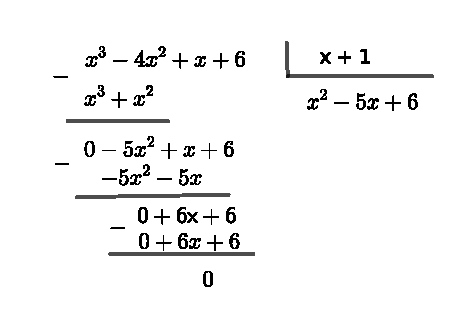
\includegraphics[width=8cm]{../Topicos/Figuras/polinomiosdivisao.pdf}
 \end{figure}
 
 note que o quociente da divisão é $q_1(x)= x^2 - 5x + 6$, e o resto desta divisão é $r(x)=0$ (zero). Como o resto é zero concluímos que $p_1(x)$ é divisível por $g_1(x)$. Portanto $p_1(x)= q_1(x)g_1(x)$, ou seja, $x^3-4x^2+x+6= (x^2-5x+6)(x+1)$.
 \end{exem}
 
 Como consequência do teorema anterior, temos o seguinte corolário, que nos garante que no exemplo anterior $-1$ é uma raiz do polinômio $p_1(x)$.
 
 \begin{cor}
 Seja $p$ um polinômio não-nulo sobre $K$. Seja $\alpha \in K$ tal que $p(\alpha)=0$. Então, existe um polinômio $q(x)$ sobre $K$ tal que 
 \[p(x)= (x - \alpha)q(x) \ .\]
 \end{cor}
 
 Como consequência deste Corolário, todo polinômio de grau $n \geq 1$ pode ser escrito como produto de $n$ fatores de grau $1$.
 
 \begin{teo}[Teorema da Decomposição]
  Todo polinômio $p(x)= a_nx^n + a_{n-1}x^{n-1}+ \ldots + a_1x+ a_0$, com $a_n \neq 0$, pode ser escrito de forma fatorada
  \[p(x)= a_n(x - r_1)(x - r_2) \ldots (x - r_n)\]
  onde $r_1, r_2, \cdots, r_n$ são as raízes do polinômio.  
 \end{teo}


%\section{Questões}
 
 \begin{enumerate}
  \item (FEPESE - 2017) Uma empresa aluga containers para guarda de bens. Se o custo de alugar $\frac{1}{4}$ de um container é R\$ 1.400,00 mensais, quanto custa alugar $\frac{4}{5}$ deste container?
  \begin{enumerate}[a)]
  \item Mais do que R\$ 4550,00. 
  \item Mais do que R\$ 4500,00 e menos que R\$ 4550,00. 
  \item Mais do que R\$ 4450,00 e menos que R\$ 4500,00. 
  \item Mais do que R\$ 4400,00 e menos que R\$ 4450,00. 
  \item Menos do que R\$ 4400,00. 
  \end{enumerate}
  
  \item (FEPESE - 2016) Uma pessoa abastece 30 litros em seu carro e observa que o ponteiro do marcador do combustível, que indicava $\frac{1}{4}$ antes do abastecimento, passou para $\frac{2}{3}$. Portanto a capacidade total do tanque, em litros, é:
  \begin{enumerate}[a)]
  \item Maior que 73 litros.
  \item Maior que 71 e menor que 73 litros.
  \item Maior que 69 e menor que 71 litros.
  \item Maior que 66 e menor que 69 litros.
  \item Menor que 66 litros.
  \end{enumerate}
  
  \item (FEPESE - 2016) Em um concurso, a razão entre aprovados e reprovados é $\frac{2}{11}$. Se o total de pessoas que prestaram esse concurso é de 143, então o número de aprovados é igual a:
  \begin{enumerate}[a)]
  \item 18.
  \item 19.
  \item 20.
  \item 21.
  \item 22.
  \end{enumerate}
  
  \item (Inst. AOCP - 2017) Com base no conhecimento sobre operações entre números Racionais na forma de frações irredutíveis, é correto afirmar que o resultado da operação $\frac{3}{5} - \frac{2}{5} + \frac{8}{5}$  é
  \begin{enumerate}[a)]
  \item $\frac{13}{15}$.
  \item $\frac{13}{5}$.
  \item $\frac{-7}{5}$.
  \item $\frac{9}{15}$.
  \item $\frac{9}{5}$.
  \end{enumerate}
  
  \item (Inst. AOCP - 2017) Dadas as frações $A= \frac{1}{3}$, $B= \frac{3}{11}$ e $C= \frac{10}{33}$ assinale a alternativa que representa a verdadeira desigualdade.
  \begin{enumerate}[a)]
  \item $A < B < C$.
  \item $B < C < A$.
  \item $C < A < B$.
  \item $B < A < C$.
  \item $C < B < A$.
  \end{enumerate}
  
  \item (UEM - 2017) Fábio possui $48$ figurinhas e deu $\frac{1}{4}$ delas para Artur, $\frac{1}{8}$ para Bianca e $\frac{5}{12}$ para Carlos. Com quantas figurinhas Fábio ficou?
  \begin{enumerate}[a)]
  \item 8
  \item 10
  \item 12
  \item 24
  \item 26
  \end{enumerate}
  
  \item (UFSCAR - 2017) Qual o valor da expressão $(\frac{3}{2})^3 - (\frac{1}{2})^2 \times (\frac{2}{15})^{-1}$ ?
  \begin{enumerate}[a)]
  \item $\frac{3}{2}$
  \item $\frac{-3}{4}$
  \item $\frac{3}{8}$
  \item $\frac{401}{120}$
  \item $\frac{1}{2}$
  \end{enumerate}
  
  \item (NC-UFPR - 2017) Assinale a alternativa que apresenta o valor da expressão $\frac{(2^{-2} \times 16)^{\frac{1}{2}}}{2^{-1}}$.
   \begin{enumerate}[a)]
  \item 1
  \item 2
  \item 4
  \item 8
  \item 16
  \end{enumerate}
  
  \item (UniRV-Goais - 2017) Qual o resultado de $16^{\frac{1}{4}} + 4^{\frac{-1}{2}}$?
  \begin{enumerate}[a)]
  \item 3
  \item $\frac{3}{2}$
  \item 5
  \item $\frac{5}{2}$
  \end{enumerate}
  
  \item (FCC - 2017) A expressão numérica $(3,4)^{-1} \cdot 6,8 - \left[ \left(\frac{3}{2} \right)^{-1} - \left(\frac{-3}{2} \right)^{-1} \right]$ é igual a:
  \begin{enumerate}[a)]
  \item 0
  \item $\frac{-1}{4}$
  \item 1,5
  \item $\frac{-1}{2}$
  \item $\frac{2}{3}$
  \end{enumerate}
  
  \item (UFSCAR - 2017) Certa receita para $18$ porções de um cookie requer $3/4$ de xícara de açúcar mascavo, $1/2$ xícara de margarina e $180$g de chocolate em pó. Para produzir $24$ porções do mesmo cookie, devemos ajustar a receita utilizando:
   \begin{enumerate}[a)]
  \item $1$ xícara de açúcar mascavo, $2/3$ de xícara de margarina e $240$g de chocolate em pó.
  \item $2$ xícaras de açúcar mascavo, $2/3$ de xícara de margarina e $260$g de chocolate em pó.
  \item $2$ xícaras de açúcar mascavo, $4/3$ de xícaras de margarina e $240$g de chocolate em pó.
  \item $1$ xícara de açúcar mascavo, $2/3$ de xícara de margarina e $260$g de chocolate em pó.
  \item $2$ xícaras de açúcar mascavo, $2/3$ de xícara de margarina e $240$g de chocolate em pó. 
  \end{enumerate}

 
  \item (FGV - 2017) Odete comprou um saco contendo 8 dúzias de balas. A seguir, ela fez saquinhos menores com 7 balas cada um. Tendo feito o maior número possível de saquinhos, o número de balas que sobrou foi 
  \begin{enumerate}[a)]
  \item 1
  \item 2
  \item 3
  \item 4
  \item 5
  \end{enumerate}
  
  \item (FGV - 2017) Considere as frações $a= \frac{2}{5}$, $b=\frac{7}{20}$ e $c=\frac{7}{20}$. A ordem crescente dessas frações é:
  \begin{enumerate}[a)]
  \item a, b, c.
  \item b, a, c.
  \item c, a, b.
  \item b, c, a.
  \item c, b, a.
  \end{enumerate}
  
  \item (FGV - 2017) Uma fábrica de bebidas vai engarrafar todo a cerveja contida em 8 barris. Cada barril contém 150 litros de cerveja e cada garrafa tem a capacidade de 750 mililitros. Assinale a opção que indica o número de garrafas usado pela fábrica.
  \begin{enumerate}[a)]
  \item 1200
  \item 1300
  \item 1400
  \item 1500
  \item 1600
  \end{enumerate}
  
  \item (FGV - 2017) Raul tem 96 anos. Teotônio tem um terço da idade de Raul e Sara tem 9 anos a mais do que Teotônio. Assinale a opção que indica a idade de Sara.
  \begin{enumerate}[a)]
  \item 23 anos
  \item 29 anos
  \item 32 anos
  \item 39 anos
  \item 41 anos
  \end{enumerate}
  
  \item (FGV - 2017) Em certo concurso inscreveram-se 192 pessoas, sendo a terça parte, homens. Desses, apenas a quarta parte passou. O número de homens que passaram no concurso foi: 
  \begin{enumerate}[a)]
  \item 12
  \item 15
  \item 16
  \item 18
  \item 20
  \end{enumerate}
  
   \item (Sociesc - 2009) Um documento da prefeitura possui 300 páginas. Com a formatação atual do texto, cada página possui 35 linhas sendo que cada linha é composta por 60 letras. Se a formatação por modificada para 30 linhas de 50 letras cada, o documento terá:
 \begin{enumerate}
  \item 258 páginas
  \item 250 páginas
  \item 420 páginas
  \item 500 páginas
 \end{enumerate}
 
 \item (Sociesc - 2009) A direção de uma escola resolveu presentear a vitória de seus alunos em uma olimpíada esportiva, com os fichários que os alunos usariam no próximo ano. Foram 32 alunos que ganharam o
 prêmio. O funcionário responsável pela compra e distribuição dos fichários, comprou 9 pacotes com 12 fichários cada. Cada aluno utiliza 4 fichários durante o ano.

 Pode-se afirmar que a quantidade planejada pelo funcionário é inadequada, pois:
 \begin{enumerate}
  \item faltarão 20 fichários para que cada aluno receba seus 4 fichários.
  \item faltarão 8 fichários para que cada aluno receba seus 4 fichários.
  \item cada aluno receberá seus 4 fichários e ainda sobrarão 6 fichários.
  \item cada aluno receberá seus 4 fichários e ainda sobrarão 12 fichários.
 \end{enumerate}
 
 \item (Sociesc - 2010) Determine o número racional $\frac{x}{y}$ sendo:
  $x=\frac{0,3 + \frac{1}{4}}{0,01}$ e $y=\frac{2-\frac{1}{3}}{0,1+6}$
  \begin{enumerate}
  \item 2013
  \item 204,2
  \item 201,3
  \item 2018
  \item 207,3
 \end{enumerate}
 
 \item (Sociesc - 2010) Em um determinado congestionamento de 6 km, cada carro ocupa 4,5 metros, em média, incluindo o pequeno espaço que separa um carro do outro. Quantos carros há neste congestionamento?
  \begin{enumerate}
  \item 1333 carros
  \item 1330 carros
  \item 1352 carros
  \item 1335 carros
  \item 1323 carros
 \end{enumerate}
 
 \item (Sociesc - 2008) Uma empresa tem dois reservatórios cúbicos de água: reservatório A, com lado igual a 1 metro e o reservatório B, com lado igual a 2 metros. Duas torneiras, torneira X e torneira Y, enchem de água os reservatórios cúbicos A e B, respectivamente. Sabendo-se que a torneira X tem vazão de 1 litro por hora, podemos afirmar que a vazão da torneira Y, para encher o recipiente B na metade do tempo que a torneira X enche o recipiente A, deve ser de:
  \begin{enumerate}
  \item 10 l/h
  \item 16 l/h
  \item 14 l/h
  \item 12 l/h
 \end{enumerate}
 
 \item (Sociesc - 2008) O número total de refrigerantes vendidos por uma cadeia de lanchonetes está aumentando exponencialmente. Se 4 bilhões de refrigerantes foram vendidos em 2000 e 12 bilhões foram vendidos no ano 2005, podemos afirmar que no ano de 2010, serão vendidos:
  \begin{enumerate}
  \item 26 bilhões
  \item 36 bilhões
  \item 42 bilhões
  \item 30 bilhões
 \end{enumerate}
 
 \item (Lógica - Fundatec - 2018) O funcionário de uma empresa constatou que, no mês de dezembro, gastou $\frac{1}{4}$ do seu salário em alimentação, $\frac{1}{5}$ do seu salário em transporte e $\frac{1}{3}$ do seu salário em moradia. Portanto, podemos conlcuir que:
\begin{enumerate}[a)]
\item Esse funcionário gastou todo o seu salário exclusivamente em alimentação, transporte e moradia.
\item Se o funcionário gastou R\$ 800,00 em alimentação então gastou R\$ 1.000,00 em moradia.
\item Se o funcionário gastou R\$ 1.200,00 em transporte então gastou R\$ 2.000,00 em moradia.
\item Se o funcionário gastou R\$ 400,00 em alimentação então gastou R\$ 500,00 em moradia.
\item Se o salário do funcionário é de R\$ 1.600,00 então ele gastou R\$ 360,00 em transporte.
\end{enumerate}

 \item (UFPE/Covest - 2015) Joana gastou $4/7$ do que havia em sua poupança comprando móveis; com o restante comprou um aparelho de TV. Se o aparelho de TV custou R\$ 1.200,00, quanto custaram, em reais, os móveis?
 \begin{enumerate}
 \item R\$ 1.300,00
 \item R\$ 1.400,00
 \item R\$ 1.500,00
 \item R\$ 1.600,00
 \item R\$ 1.700,00
 \end{enumerate}
 
 \item (UFPE/Covest - 2015) Usando 42 linhas por página e 78 caracteres (ou espaços) em cada linha, um texto ocupa 54 páginas. Para melhorar a legibilidade do texto, diminuiu-se para 26 o número de linhas por página e para 63 o número de caracteres (ou espaços) por linha. Qual será o número de páginas ocupadas pelo texto na nova configuração?
 \begin{enumerate}
 \item 100 
 \item 102
 \item 104
 \item 106
 \item 108
 \end{enumerate}

 \end{enumerate}
 
 Gabarito: 1 c); 2 b); 3 e); 4 e); 5 b); 6 b); 7 a); 8 c); 9 d); 10 e); 11 a); 12 e); 13 d); 14 e); 15 e); 16 c); 17 c); 18 a); 19 c); 20 a); 21 b); 22 b); 23 c); 24 d); 25 e).


\maketitle

\chapter{Equações}
%\label{cap:0}

\colorbox{azul}{
 \begin{minipage}{14.5cm}
 \begin{center}
   Uma equação é uma sentença matemática aberta, ou seja, sentença matemática que possui ao menos uma incógnita, e que estabelece uma igualdade entre duas expressões matemáticas.
 \end{center}
 \end{minipage}}
 
 \vskip0.3cm
 
 \begin{exem}
 A seguintes expressões matemáticas são exemplos de equações:

\begin{enumerate}[(1)]
 \item $x+1=3$;
 \item $\sin(x)=0$;
 \item $2x+3=7x-2$;
 \item $x^2+3x+1=0$;
 \item $x+y= 5$.
\end{enumerate}
\end{exem}

 E para ajudar a entender o conceito de equação, seguem algumas expressões matemáticas que não são equações, com a justificativa do porquê elas não são equações:
\begin{exem}
\begin{enumerate}[(1)]
 \item Uma desigualdade, ou seja, uma sentença matemática que relaciona duas expressões matemáticas através do sinal de diferente ($\neq$), não é uma equação, exemplo: $x+1 \neq 3$.
 
 \item $3 + 2 = 5$, por não ser uma sentença aberta.
 
 Sentenças matemáticas que relacionam duas expressões matemáticas através dos sinais de menor ($<$), maior ($>$), menor ou igual ($\leqq$), maior ou igual ($\geqq$), não são equações. Elas são chamadas de inequações. Seguem alguns exemplos:
 
 \item $\sin(x) < 0$, neste caso o sinal de menor $<$, nos diz que $\sin(x)$ é menor do que $0$.
 \item $2x+3 \leqq 7x-2$.
 \item $x^2+3x+1 \geqq 0$.
\end{enumerate}
\end{exem}



Vamos nos dedicar nesta seção para entender as equações de 1º grau e as de 2º grau. Mas antes vejamos um exemplo de como as equações aparecem em nosso dia-a-dia.

\begin{exem}
 Situação problema: Geraldo frequenta uma lan house, pois não tem internet em sua casa, e paga uma taxa fixa de $R\$ 1,00$ a primeira hora, mais $R\$ 2,00$ a cada hora excedente. Se após o uso Geraldo pagou $R\$ 7,00$, por quanto tempo ele usou a internet?
 
 \underline{Resolução:}
 
 Podemos concluir que Geraldo usou o computador por $4$ horas, já que pagou $R\$ 1,00$ pela primeira hora, e consequentemente $(7,00 - 1,00 = 6,00)$ $R\$ 6,00$ pelas demais horas, como cada hora a mais custa $R\$ 2,00$ e $(6,00 \div 2,00 = 3)$ temos então que Geraldo usou $(1 + 3 = 4)$ horas.
 
 Podemos generalizar esta situação usando a letra $x$ para representar o tempo de internet utilizado, que é o valor que não conhecemos, chegando à seguinte equação: $2x + 1 = 7$.
\end{exem}

A equação resultante desta situação problema é o que chamamos de equação do 1º grau.

\section{Equações do 1º grau}

\colorbox{azul}{
 \begin{minipage}{14.5cm}
 \begin{center}
   As equações de 1º grau tem a seguinte forma geral:
 \[ax + b = 0\]
onde $a, b \in \mathbb{R}$ são números dados (conhecidos), com $a \neq 0 $.
 \end{center}
 \end{minipage}}
 
 \vskip0.3cm

Como resolver uma equação destas, ou equivalentemente, como encontrar o valor de $x$: 
\[ax + b = 0 \Rightarrow ax= -b \Rightarrow x = \frac{-b}{a} \ .\]


\begin{exem}
 Como resolver equações do 1º grau:
 \begin{itemize}
  \item $2x + 4 = 0 \Rightarrow 2x = -4 \Rightarrow x = \frac{-4}{2} \Rightarrow x = -2$
  \item $3x - 5 = 4 \Rightarrow 3x = 4 +5 \Rightarrow 3x = 9 \Rightarrow x = \frac{9}{3} \Rightarrow x = 3$
  \item $3(x + 2)= 12 \Rightarrow 3x + 6 = 12 \Rightarrow 3x = 12 - 6 \Rightarrow 3x = 6 \Rightarrow x = \frac{6}{3} \Rightarrow x = 2 $
  \item $ax = 0$ 
  
  Neste caso $a \neq 0$, como produto de dois números só é zero quando um deles for igual a zero concluímos que $x = 0$.
  \end{itemize}
\end{exem}

\section{Equações do 2º grau}

\colorbox{azul}{
 \begin{minipage}{14.5cm}
 \begin{center}
   As equações de 2º grau tem a seguinte forma geral:
   \[ax^2 + bx + c = 0\]
  onde $a, b, c \in \mathbb{R}$ são números dados (conhecidos), com $a \neq 0 $.
 \end{center}
 \end{minipage}}

 \vskip0.3cm
 
Para resolver este tipo de equação usamos a famosa fórmula de Báskara, que não foi criada por ele, mas acabou recebendo este nome em algum momento da história, dada por:
 
 \vskip0.3cm
 \begin{center}
 \textbf{Fórmula de Báskara}
   \[\destaque{x= \frac{-b \pm \sqrt{b^2 - 4ac}}{2a}}\]
 \end{center}

O sinal $\pm$ que aparece antes da raíz quadrada na equação acima é justificado se você notar que: extrair a raíz quadrada de um número $y$ é procurar o número $z$ tal que $z^2 = y$, assim observe que pelas propriedades de potência se $z^2= y$ então $(-z)^2= y$ donde obtemos que $\sqrt{y} = \pm z$.

\vskip0.3cm

\textbf {Exemplo de aplicação das equações do 2º grau.}

\begin{exem}
 Uma mesa de sinuca de $R\$ 360,00$ devia ser comprada por um grupo de rapazes que contribuíam em partes iguais. Como quatro deles desistiram, a quota de cada um dos outros ficou aumentada de $R\$ 15,00$. Quantos eram os rapazes?
 
 \underline{Resolução:}
 
 Se chamarmos de $x$ a quantidade inicial de rapazes, cada um contribuia com a quantidade de $\frac{360}{x}$. Com a desistência de 4 rapazes, a nova quota a ser paga seria de $\frac{360}{x - 4}$. E como o problema nos informa a nova quota é $R\$ 15,00$ maior que a anterior, podemos escrever:
 \[\frac{360}{x - 4} - \frac{360}{x} = 15\]
 Simplificando ambos os membros por $15$, podemos escrever
 \[\frac{24}{x - 4} - \frac{24}{x} = 1\]
 Assim, tirando o MMC chegamos:
 \begin{equation*}
  \Rightarrow \frac{24 x - 24(x-4)}{(x - 4)x} = 1 \Rightarrow \frac{24x - 24x + 96}{x^2 - 4x} = 1 
  \Rightarrow 96 = x^2 - 4x \Rightarrow x^2 - 4x - 96 = 0 
 \end{equation*}

 Agora utilizando a fórmula da equação do segundo grau é possível encontrar o valor de $x$ que é a quantidade inicial de rapazes, façamos isso então. Lembre-se que a fórmula geral da equação do 2º grau é $ax^2 + bx + c = 0$ assim, neste caso temos que $a = 1$, $b = -4$ e $c = -96$, portanto substituindo na fórmula:
 
 \[ x= \frac{-b \pm \sqrt{b^2 - 4ac}}{2a} \]
 
 \begin{eqnarray*}
  x= \frac{-(-4) \pm \sqrt{(-4)^2 - 4(1)(-96)}}{2(1)} \Rightarrow 
  x = \frac{4 \pm \sqrt{16 + 384}}{2} \Rightarrow
  x = \frac{4 \pm \sqrt{400}}{2}
 \end{eqnarray*}

\[ \Rightarrow x = \frac{4 \pm 20}{2} \Rightarrow \begin{cases}
                                                  x' = \frac{4 + 20}{2} \Rightarrow x' = \frac{24}{2} \Rightarrow x' = 12 \\
                                                  x'' = \frac{4 - 20}{2} \Rightarrow x'' = \frac{-16}{2} \Rightarrow x'' = -8
                                                 \end{cases}\]

Como nossa situção problema é saber quantidade inicial de rapazes não faz sentido $x < 0$, donde concluímos que $x = 12$. 
\fim
\end{exem}



\begin{exem}
 Como resolver equações do 2º grau:
 \begin{itemize}
  \item Equação do 2º grau completa do tipo $ax^2 + bx + c = 0$.
  
  Feito na situação problema acima.
  \item Equação do 2º grau incompleta do tipo $ax^2 + bx = 0$
  \[x^2 - 3x = 0\]
  1ª forma:
  
  $a = 1$, $b = -3$ e $c = 0$ assim usando a fórmula chegamos:
  \[x = \frac{- (-3) \pm \sqrt{(-3)^2 - 4 (1)(0)}}{2 (1)}\]
  \[\Rightarrow x = \frac{3 \pm \sqrt{9}}{2} \Rightarrow \begin{cases}
                                                          x' = \frac{3 + 3}{2} \Rightarrow x' = \frac{6}{2} \Rightarrow x' = 3 \\
                                                          x'' = \frac{3 - 3}{2} \Rightarrow x''= \frac{0}{2} \Rightarrow x''= 0
                                                         \end{cases}\]
  
  2ª forma:
  \[x^2 - 3x = 0 \Rightarrow x(x - 3)=0 \Rightarrow \begin{cases}
                                                     x''= 0 \\
                                                     x - 3 = 0 \Rightarrow x' = 3
                                                    \end{cases}\]
 
  
  \item Equação do 2º grau incompleta do tipo $ax^2 + c = 0$
  \[2x^2 - 128 = 0\]
  1ª forma:
  
  $a = 2$, $b = 0$ e $c = -128$ assim usando a fórmula chegamos:
  \[x = \frac{- (0) \pm \sqrt{(0)^2 - 4 (2)(-128)}}{2 (2)}\]
  \[\Rightarrow x = \frac{0 \pm \sqrt{1024}}{4} \Rightarrow \begin{cases}
                                                          x' = \frac{ 0 + 32}{4} \Rightarrow x' = \frac{32}{4} \Rightarrow x' = 8 \\
                                                          x'' = \frac{0 - 32}{4} \Rightarrow x''= \frac{-32}{4} \Rightarrow x''= -8
                                                         \end{cases}\]
  
  
  2ª forma:
  \[2x^2 - 128 = 0 \Rightarrow 2x^2 = 128 \Rightarrow x^2 = \frac{128}{2} \Rightarrow x^2 = 64 \Rightarrow x = \pm \sqrt{64} \Rightarrow x = \pm 8\]
  
  \item Equação do 2º grau incompleta do tipo $ax^2 = 0$.
  
  Neste caso $a \neq 0$, como produto de dois números só é zero quando um deles for igual a zero concluímos que $x^2 = 0 \Rightarrow x =0$.
  \end{itemize}
\end{exem}

\section{Equações exponenciais}

  \vskip0.3cm
 \colorbox{azul}{
 \begin{minipage}{14.5cm}
 \begin{center}
  As equações exponenciais são aquelas em que a incógnita aparece nos expoentes.
 \end{center}
 \end{minipage}}
 \vskip0.3cm
 
 Como por exemplo nas equações:
 \[3^x= 9 \ ,\]
 \[4^{x+1}= 256 \ ,\] 
 \[3^{2x}- 18\cdot 3^x + 81=0 \ .\]
 
 Para resolver equações como estas é muito importante dominar:
 \begin{itemize}
  \item resolução de equações de 1º grau e de 2ª grau;
  \item propriedades de potência.
 \end{itemize}
 
 Existem duas formas de resolver as equações exponenciais, são elas: método da redução a uma base comun e logaritmos. Abordaremos agora o primeiro caso.
 
 \vskip0.3cm
 
 \textbf{Método da redução a uma base comum}
 
 \vskip0.3cm
 
 O caso mais simples de equações exponencias são as equações do tipo 
 \[\destaque{a^{x}= b} \ ,\]
 para $a > 0 \text{ e } a \neq 1 \in \R$. Note que com esta restrição de $a$ teremos sempre $b > 0 \in \R$ e ainda que esta equação está definida para todo $x \in \R$. 
 
 Deste caso mais simples decorre que as equações exponenciais de base $a$ estão definidas apenas para $a > 0 \text{ e } a \neq 1 \in \R$. A resolução das equações $a^x= b$ pelo método da redução a uma base comum consiste em escrever $b$ como uma potência de $a$, ou seja, $b= a^k$  para algum $k \in \R$, e portanto $a^{x}= b= a^{k} \Rightarrow x= k$.
  
 Portanto, a seguinte propriedade é essencial na resolução de equações exponenciais:
 
 \[\destaque{ a^{x_1}= a^{x_2} \Rightarrow x_1= x_2 \text{ para } a>0 \text{ e } a \neq 1}\]
 
 \begin{exem}
  Consideremos a equação $3^x= 9$.
  
  \begin{tabular}{c|c}
  9 & 3 \\
  3 & 3 \\
  1 &   
  \end{tabular}
  
  Portanto ao fatorar o número 9 obtemos $9= 3^2$, assim $3^x= 3^2 \Rightarrow x= 2$.
 \end{exem}
 
 \begin{exem}
  Consideremos a equação $4^{x+1}= 256$.
  
  \begin{tabular}{c|c}
   256 & 2 \\
   128 & 2 \\
   64  & 2 \\
   32  & 2 \\
   16  & 2 \\
   8   & 2 \\
   4   & 2 \\
   2   & 2 \\
   1   &   \\
  \end{tabular}
  
  Neste caso ao fatorar 256 obtemos $256=2^8 =4^4$, assim 
  \begin{eqnarray*}
  4^{x+1}= 4^4 \Rightarrow x+1= 4 \Rightarrow x= 4-1 \Rightarrow x=3 \ .
  \end{eqnarray*}

 \end{exem}
 
 \begin{exem}
  Consideremos a equação $3^{2x}- 18\cdot 3^x + 81=0$.
  
  Para resolver esta equação façamos $y= 3^x$, substituindo na equação acima temos
  \begin{eqnarray*}
   3^{2x} - 18\cdot 3^x + 81&=& 0 \\
   (3^x)^2 - 18\cdot 3^x + 81&=& 0 \\
   y^2 - 18y + 81 &=& 0
  \end{eqnarray*}
  
  Resolvendo esta equação de 2º grau temos:
  \begin{eqnarray*}
   y &=& \frac{18 \pm \sqrt{324 - 4.81}}{2.1} \\
   \Rightarrow y&=& \frac{18 \pm \sqrt{0}}{2} \\
   \Rightarrow y&=& \frac{18}{2} \Rightarrow y= 9
  \end{eqnarray*}
  
  Portanto, como $y= 9$ e $y= 3^x$ obtemos que $3^x= 9$ e como já vimos resulta em $x= 2$.

 \end{exem}
 
 \begin{exem}
  Vamos agora resolver a equação $9^x= \frac{1}{81}$.
  
  \begin{tabular}{c|c}
   81 & 3 \\
   27 & 3 \\
   9  & 3 \\
   3  & 3 \\
   1  &   \\
  \end{tabular}

  Neste caso, temos que $81= 9^2$, assim 
  \[\frac{1}{81}= \frac{1}{9^2}= 9^{-2} \ ,\]
  que substituindo na equação exponencial nos dá, 
  \[9^x= 9^{-2} \Rightarrow x= -2 \ .\]
 \end{exem}
 
 \begin{exem}
  Considera a equação $(49)^{x+2}= \frac{1}{7^3}$.
  
  \begin{tabular}{c|c}
   49 & 7 \\
   7  & 7 \\
   1  &   \\
  \end{tabular}
  
  Fatorando o $49$ obtemos que $49= 7^2$, portanto
  \[(49)^{x+2}= (7^2)^{x+2}= 7^{2\cdot (x+2)}\]
  que substituindo na equação nos leva à:
  \begin{eqnarray*}
   7^{2\cdot (x+2)}= \frac{1}{7^3} \\
   7^{2\cdot (x+2)}= 7^{-3} \\
   2\cdot (x+2) = -3 \\
   2x + 4 = -3 \\
   2x= -3 -4 \\
   x= \frac{-7}{2}
  \end{eqnarray*}

 
 \end{exem}






\newpage

\section{Exercícios de fixação}

 Antes de tentar resolver situações problema envolvendo equações vamos treinar um pouco a resolução das equações resolvendo os seguintes exercícios.
 
  Para fixar a teoria resolva as seguintes equações de 1º grau:
 \begin{multicols}{2}
  \begin{enumerate}[a)]
   \item $x + 4= 10$ 
   \item $x - 8= -10$
   \item $9x= 18$
   \item $7x - 1 =20$
   \item $2x + 6= x + 18$
   \item $3(x + 2)= 15$
   \item $2(x-1)-7= 16$
   \item $2(x-6)= -3(5+x)$
   \item $3(2x-3) + 2(x+1)= 3x + 18$
   \item $2(x+1)- 3(2x-5)= 4x + 9$
   \item $2x-(x-1)=5-(x-3)$
   \item $\frac{x}{5}+ 5= \frac{x}{4} + 4$
   \item $\frac{x}{3} - 2= \frac{x}{5}$
   \item $\frac{3}{x-4}= \frac{-4}{2x+7}$
   \item $\frac{3x+4}{5x-2}= \frac{7}{3}$
 \end{enumerate}
 \end{multicols}
 
  Para fixar a teoria resolva as seguintes equações de 2º grau:
 \begin{multicols}{2}
  \begin{enumerate}[a)]
   \item $x^2 + 4= 20$ 
   \item $(x - 8)^2= -10$
   \item $9x^2= 81$
   \item $x^2 - 3x= 0$
   \item $(x + 13)^2= 0$
   \item $(x + 2)(x - 81)= 0$
   \item $(x-1)(x-7)= 16$
   \item $2x^2-2x-24= 0$
   \item $2x^2+16x= 0$
   \item $2x^2+2x-112= 0$
   \item $x^2-6x+13= 0$
   \item $\frac{x}{5}+ 5= \frac{x}{4} + 4$
   \item $\frac{x}{3} - \frac{4}{2x}= \frac{x}{5}$
   \item $\frac{3}{x-4}= \frac{2x+7}{-4}$
   \item $\frac{7}{5x-2}= \frac{3x+4}{3}$
 \end{enumerate}
 \end{multicols}
 
 Para fixar a teoria resolva as seguintes equações exponenciais:
 \begin{multicols}{2}
  \begin{enumerate}[a)]
   \item $3^x= 243$
   \item $5^x= \frac{1}{125}$
   \item $2^{x+3}= 64$
   \item $3^x= 1$
   \item $5^{x-2}= 25$
   \item $2^{2x+3}= 8$
   \item $(4)^{3x-2}= \frac{1}{8}$
   \item $(4)^{3x-2}= 32$
   \item $4^{2x} - 32\cdot 4^x + 256 = 0$
   \item $5^{2x} - 50 \cdot 5^x + 625=0$
   \item $\left(\frac{1}{16} \right)^{x-2}= 8^x$
   \item $(0,25)^{x-1}= \left(\frac{1}{8} \right)^{1-x}$
  \end{enumerate}
  \end{multicols}
 
\newpage

%\section{Questões}
 
\begin{enumerate}
 \item (VUNESP - 2017) Uma sorveteria vende os sorvetes em copinhos pequenos, médios ou grandes, cuja soma dos respectivos preços unitários é igual a $R\$ 42,00$. Sabe-se que os preços unitários dos copinhos médio e grande correspondem, respectivamente, a $\frac{7}{4}$ e $\frac{5}{2}$ do preço do copinho pequeno. Desse modo, é correto afirmar que cada copinho grande é vendido por
 \begin{multicols}{5}
 \begin{enumerate}[a)]
 \item $R\$ 16,00$
 \item $R\$ 16,50$
 \item $R\$ 18,50$
 \item $R\$ 20,00$
 \item $R\$ 21,00$
 \end{enumerate}
 \end{multicols}
 
 \item (IBFC - 2017) Alípio foi ao hortifruti e comprou laranjas e limões, no total de $22$ unidades. O número de laranjas é igual ao número de limões diminuído de $6$ unidades. Desse modo, o número de limões comprados por Alípio foi:
 \begin{multicols}{5}
 \begin{enumerate}[a)]
 \item $8$
 \item $10$
 \item $14$
 \item $16$
 \item $17$
 \end{enumerate}
 \end{multicols}
 
 \item (UVA - 2016) Dois amigos praticam um jogo mental usando números decimais. José diz um número natural qualquer e Tiago deve multiplicá-lo por $0,6$, depois somar $3,2$ e, por fim, dividir este resultado por $0,5$. Se Tiago obteve $12,4$, então o número dito por José foi:
 \begin{multicols}{5}
 \begin{enumerate}[a)]
 \item $4$
 \item $5$
 \item $6$
 \item $7$
 \end{enumerate}
 \end{multicols}
 
 \item (NC-UFPR - 2017) Considere a equação dada por $2x^2 + 12x + 3 = -7$. Assinale a alternativa que apresenta a soma das duas soluções dessa equação.
 \begin{multicols}{5}
 \begin{enumerate}[a)]
 \item $0$
 \item $1$
 \item $-1$
 \item $6$
 \item $-6$
 \end{enumerate}
 \end{multicols}
 
 \item (UEM - 2017) Se $m$ e $n$ são as soluções da equação  $2x^2 +9x - 5 = 0$  e $m$ é maior do que $n$, então o valor de $n +10m$ é igual a
 \begin{multicols}{5}
 \begin{enumerate}[a)]
 \item $0$
 \item $5$
 \item $-5$
 \item $10$
 \item $-10$
 \end{enumerate}
 \end{multicols}

 \item (PUC-PR - 2017) A equação $8x^2 – 28x + 12 = 0$ possui raízes iguais a $x_1$ e $x_2$. Qual o valor do produto $x_1 \cdot x_2$?
 \begin{multicols}{5}  
 \begin{enumerate}[a)]
 \item $\frac{1}{2}$
 \item $3$
 \item $\frac{3}{2}$
 \item $12$
 \item $28$
 \end{enumerate}
 \end{multicols}
 
 \item (IBFC - 2017) A alternativa que apresenta a equação de 2.º grau cujas raízes reais são $5$ e $(-1)$ é:
 \begin{enumerate}[a)]
 \item $x^2 + 4x + 5 = 0$
 \item $x^2 + 4x^2 – 5 = 0$
 \item $2x^2 - 2x + 10 = 0$
 \item $2x^2 + 2x – 10 = 0$
 \item $x^2 - 4x – 5 = 0$
 \end{enumerate}
 
 \item (UNISUL - 2016) Considere as proposições:
 \begin{enumerate}[I)]
 \item O valor de $350^2 - 349^2 = 1$.
 \item O valor numérico da expressão  $x^2+ 2x + 1 / x+1$ quando $x = 1523$ é $1524$.
 \item A igualdade $4x^2 - 36 / 2x + 6 = 2x - 6$ , para todo $x \in \R$.
 \item $(√3 + 5)2 = (√3)2 + 52 = 3 + 25 =28$.
 \end{enumerate}
 É(são) verdadeira(s) a(s) proposição(ões):
 \begin{enumerate}[a)]
 \item I, II e IV.
 \item Apenas a I.
 \item Apenas a III.
 \item II e III.
 \item Apenas a II.
 \end{enumerate}
 
 \item (UNISUL - 2016) Sejam $r$ e $s$ as raízes da equação $x^2 - 9x + 13 = 0$, assinale a alternativa que corresponde ao valor numérico da expressão $(r + s)^2 + 4rs$.
 \begin{multicols}{5}
 \begin{enumerate}[a)]
 \item 131.
 \item 129.
 \item 130.
 \item 133.
 \item 132.
 \end{enumerate}
 \end{multicols}
 
 \item (COPESE-UFPI - 2016) Djair está casado há $m$ anos. Se ele permanecer casado por mais $30$ anos, ele irá estar casado por $m^2$ anos. Pode-se afirmar que Djair já está casado há:
 \begin{multicols}{5}
 \begin{enumerate}[a)]
 \item 3 anos.
 \item 4 anos.
 \item 5 anos.
 \item 6 anos.
 \item 7 anos.
 \end{enumerate}
 \end{multicols}
 
 \item (Sociesc - 2010) Em uma cidade existem duas locadoras de automóveis. A locadora A cobra uma taxa fixa de R\$ 50,00 por dia e R\$ 1,50 por quilômetro rodado. A locadora B cobra uma taxa fixa de R\$ 30,00 por dia e R\$ 2,00 por quilômetro rodado. Sendo assim, podemos afirmar que, em um dia:
  \begin{enumerate}
  \item A locadora B é mais vantajosa somente para um percurso superior a 40 quilômetros.
  \item Para qualquer quilometragem é sempre vantagem usar a locadora A.
  \item Para qualquer quilometragem é sempre vantagem usar a locadora B.
  \item O preço é o mesmo nas duas locadoras independente da quilometragem.
  \item A locadora A é mais vantajosa somente para um percurso superior a 40 quilômetros. 
 \end{enumerate}

\item (Sociesc - 2009) Quando $\sqrt{x + \sqrt{2x+3}}= \sqrt{4x-6}$ o valor de $-x^2+1$ é:
 \begin{enumerate}
  \item 10
  \item $\frac{11}{9}$
  \item $\pm 1$
  \item -8
 \end{enumerate}
 
 \item (Sociesc - 2009) Na equação $ax^2+bx+c-k=0$ tem-se os seguintes valores para o par $(x, k): (0,-1), (2,-1) \text{ e } (-1,-4)$. Nessas condições, a(s) raízes da equação quando $k=0$ podem ser expressa(s) como:
 \begin{enumerate}
  \item $\pm 1$
  \item 1
  \item -1
  \item 0
 \end{enumerate}
 
 \item (Sociesc - 2009) João perguntou à sua irmã quantos metros de fita dupla face deveria comprar, para prender uma toalha em uma mesa retangular, na festa de rua que estavam organizando. Sua irmã deu-lhe a seguinte resposta: a mesa retangular tem 3 metros a mais de comprimento que a largura. Como a área da mesa é $10 m^2$, concluímos que seu perímetro é:
  \begin{enumerate}
  \item 14 metros
  \item 15 metros
  \item 13 metros
  \item 16 metros
 \end{enumerate}
 
 \item (Sociesc - 2009) Existem dois números, $x_1$ e $x_2$ , que satisfazem a seguinte condição: "o seu quadrado é igual ao seu triplo”. A soma de $x_1$ e $x_2$ é:
  \begin{enumerate}
  \item 5
  \item 2
  \item 4
  \item 3
 \end{enumerate}
 
 \item (Sociesc - 2010) A soma das raízes das equações $\frac{x}{6}+\frac{x}{3}=18$ e $4x^2-64=0$ é igual a:
  \begin{enumerate}
  \item 40
  \item -36
  \item 44
  \item -44
  \item 36
 \end{enumerate}
 
  \item (Sociesc - 2010) Pense em um número, disse João a Pedro, e faça o que eu pedir, pois vou adivinhar o resultado das operações matemáticas feitas com o número que você pensou. Pedro pensou num número e João começou a dizer as operações que ele deveria fazer: calcule o dobro do número que você pensou e some 7 unidades; multiplique este resultado por 4, subtraia 28 e divida o resultado pelo próprio número. Após Pedro ter feito os cálculos, João olhou para ele e “adivinhou” que o resultado era:
  \begin{enumerate}
  \item 8 
  \item -8
  \item 4
  \item -4
  \item 10
 \end{enumerate}
 
 \item (Sociesc - 2010) O ponto do eixo das \sout{abscissas} (ordenadas) equidistante dos pontos $A(-1, 1)$ e $B(3, 2)$ é:
  
 
 \begin{multicols}{2}
 
 \begin{enumerate}
  \item $(0, \frac{15}{2})$
  \item $(0, \frac{9}{2})$
  \item $(0,5)$
  \item $(0, \frac{17}{2})$
  \item $(0, \frac{11}{2})$
 \end{enumerate}
 
 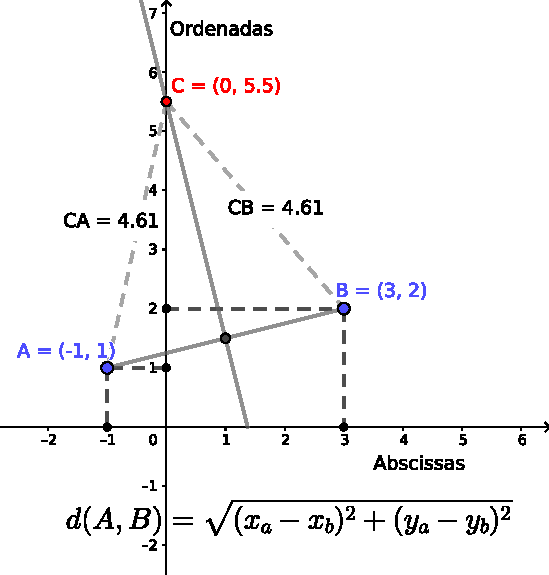
\includegraphics[width=5cm]{../../Topicos/Figuras/dist_exer1.pdf} 
 
 \end{multicols}
 
 \item (Sociesc - 2009) Um fazendeiro dividirá seu terreno em três partes para plantar milho, soja e trigo. A área onde será plantado o milho terá o dobro da área onde será plantada a soja, que por sua vez terá o dobro da área do trigo. O terreno tem área de 42 hectares. As áreas reservadas para a plantação do milho, da soja e do trigo, serão, respectivamente:
  \begin{enumerate}
  \item 12, 24 e 6 hectares
  \item 20, 10 e 2 hectares
  \item 14, 14 e 14 hectares
  \item 24, 12 e 6 hectares
 \end{enumerate}
 
 \item (SOCIESC - Téc. Enfermagem) Na prova da matéria X, o professor decidiu colocar 20 questões, das quais cada certa vale 1 ponto e cada errada decresce 0,5 pontos. Assim, uma pessoa que acertou 12 questões obteve a nota:
  \begin{enumerate}
  \item Mínima
  \item Maior do que 7
  \item Maior do que 10
  \item Menor do que 7
  \item Máxima
 \end{enumerate}
 
 \item (SOCIESC - Téc. Enfermagem) O valor de $x$ em: $4x-7=2(3x-8)$ é:
 \begin{enumerate}
  \item 4,5
  \item 18
  \item 0,5
  \item 0,3
  \item 2
 \end{enumerate}
 
 \item (Lógica - Fundatec - 2018) Uma locadora de máquinas de café expresso cobra uma taxa diária de R\$ 83,00 e R\$ 0,30 por café de 50ml produzido. Quanto pagaria a organização de um evento na locação de um máquina durante 5 dias se produzisse 400 cafés expressos de 50ml?
\begin{multicols}{2}
\begin{enumerate}[a)]
\item 490,00
\item 535,00
\item 1.615,00
\item 6.000,00
\item 6.415,00
\end{enumerate}
\end{multicols}

 \item (UDESC/IBC - 2009) Se $x$ e $y$ são números reais tais que $2x + y = 8$, o valor máximo do produto $x \cdot y$ é:
 \begin{enumerate}
 \item 24
 \item 20
 \item 16
 \item 12
 \item 8
 \end{enumerate}
 
 \item (UDESC/IBC - 2009) Para que valores de $m$ a equação $4x^2- 4mx + (4m – 3) = 0$ não admite raízes reais?
 \begin{enumerate}
 \item $\{m \in \R \mid 1< m < 3\}$
 \item $\{\forall m \mid m \in \R\}$
 \item $\{m \in \R \mid m < 1 \text{ ou } m > 3\}$
 \item $m > 0$
 \item nenhum valor real de $m$.
 \end{enumerate}
 
 \item (TJ/SC - 2018) Em uma fila há 70 pessoas, entre as quais Pedro e João. Sabe-se que:
  \begin{itemize}
   \item Pedro está na frente de João e há duas pessoas entre eles;
   \item O número de pessoas na frente de Pedro é o dobro do número de pessoas atrás de João.
  \end{itemize}
  Nessa fila João ocupa o:
  \begin{enumerate}
  \item 45ª lugar
  \item 46ª lugar
  \item 47ª lugar
  \item 48ª lugar (*)
  \item 49ª lugar
 \end{enumerate}
 
 \end{enumerate}
 
 Gabarito: 1 d); 2 c); 3 b); 4 e); 5 a); 6 c); 7 e); 8 d); 9 d); 10 d); 11 e); 12 d); 13 b); 14 a); 15 d); 16 e); 17 a); 18 e); 19 d); 20 b); 21 a); 22 b); 23 e); 24 a).
 


\chapter{Funções}

\section{Definição de funções}

\vskip0.3cm
 \colorbox{azul}{
 \begin{minipage}{0.9\linewidth}
 \begin{center}
  Dados dois conjuntos $A$ e $B$ não vazios, de números Reais, ou seja, $A \subseteq \mathbb{R}$ e $B \subseteq \mathbb{R}$. Uma \textbf{aplicação} de $A$ em $B$ ou \textbf{função} definida no conjunto $A$ com imagens em $B$ é uma regra (equação) que diz como associar cada elemento $x \in A$ a um \underline{único} $y \in B$.
 \end{center}
 \end{minipage}}
 \vskip0.3cm


 Exemplos de relações que são funções de $A$ em $B$:
 \begin{multicols}{3}
 \begin{tikzpicture}
 \node (1) at (0,0) {1};%\filldraw(1.east) circle (1pt)
 \node (2) [below of=1] {2};%\filldraw(2.east) circle (1pt)
 \node (3) [below of=2] {3};%\filldraw(3.east) circle (1pt)
 \node[fit=(1) (2) (3),ellipse,draw=red,minimum width=1cm,thick,label=below:\(A\)]{};

 \node (a) at (3,0) {a};%\filldraw($b_1$.west) circle (1pt)
 \node (b) [below of=a] {b};%\filldraw($b_2$.west) circle (1pt)
 \node (c) [below of=b] {c};%\filldraw($b_3$.west) circle (1pt)
 \node[fit=(a) (b) (c),ellipse,draw=green,minimum width=1cm,thick,label=below:\(B\)]{};

 \draw[->, shorten >=.1cm, >=stealth'] (1.east) to (a.west);
 \draw[->, shorten >=.1cm, >=stealth'] (2.east) to (b.west);
 \draw[->, shorten >=.1cm, >=stealth'] (3.east) to (c.west);
\end{tikzpicture} \\
 \begin{tikzpicture}
 \node (1) at (0,0) {1};%\filldraw(1.east) circle (1pt)
 \node (2) [below of=1] {2};%\filldraw(2.east) circle (1pt)
 \node (3) [below of=2] {3};%\filldraw(3.east) circle (1pt)
 \node[fit=(1) (2) (3),ellipse,draw=red,minimum width=1cm,thick,label=below:\(A\)]{};

 \node (a) at (3,0) {a};%\filldraw($b_1$.west) circle (1pt)
 \node (b) [below of=a] {b};%\filldraw($b_2$.west) circle (1pt)
 \node (c) [below of=b] {c};%\filldraw($b_3$.west) circle (1pt)
 \node[fit=(a) (b) (c),ellipse,draw=green,minimum width=1cm,thick,label=below:\(B\)]{};

 \draw[->, shorten >=.1cm, >=stealth'] (1.east) to (a.west);
 \draw[->, shorten >=.1cm, >=stealth'] (2.east) to (a.west);
 \draw[->, shorten >=.1cm, >=stealth'] (3.east) to (c.west);
\end{tikzpicture} \\
\begin{tikzpicture}
 \node (1) at (0,0) {1};%\filldraw(1.east) circle (1pt)
 \node (2) [below of=1] {2};%\filldraw(2.east) circle (1pt)
 \node (3) [below of=2] {3};%\filldraw(3.east) circle (1pt)
 \node[fit=(1) (2) (3),ellipse,draw=red,minimum width=1cm,thick,label=below:\(A\)]{};

 \node (a) at (3,0) {a};%\filldraw($b_1$.west) circle (1pt)
 \node (b) [below of=a] {b};%\filldraw($b_2$.west) circle (1pt)
 \node (c) [below of=b] {c};%\filldraw($b_3$.west) circle (1pt)
 \node[fit=(a) (b) (c),ellipse,draw=green,minimum width=1cm,thick,label=below:\(B\)]{};

 \draw[->, shorten >=.1cm, >=stealth'] (1.east) to (b.west);
 \draw[->, shorten >=.1cm, >=stealth'] (2.east) to (b.west);
 \draw[->, shorten >=.1cm, >=stealth'] (3.east) to (b.west);
\end{tikzpicture}

\end{multicols}



 Exemplos de relações que não são funções de $A$ em $B$:
\begin{multicols}{3}
\begin{tikzpicture}
 \node (1) at (0,0) {1};%\filldraw(1.east) circle (1pt)
 \node (2) [below of=1] {2};%\filldraw(2.east) circle (1pt)
 \node (3) [below of=2] {3};%\filldraw(3.east) circle (1pt)
 \node[fit=(1) (2) (3),ellipse,draw=red,minimum width=1cm,thick,label=below:\(A\)]{};

 \node (a) at (3,0) {a};%\filldraw($b_1$.west) circle (1pt)
 \node (b) [below of=a] {b};%\filldraw($b_2$.west) circle (1pt)
 \node (c) [below of=b] {c};%\filldraw($b_3$.west) circle (1pt)
 \node[fit=(a) (b) (c),ellipse,draw=green,minimum width=1cm,thick,label=below:\(B\)]{};

 \draw[->, shorten >=.1cm, >=stealth'] (1.east) to (a.west);
 \draw[->, shorten >=.1cm, >=stealth'] (1.east) to (b.west);
 \draw[->, shorten >=.1cm, >=stealth'] (2.east) to (b.west);
 \draw[->, shorten >=.1cm, >=stealth'] (3.east) to (c.west);
\end{tikzpicture} \\
\begin{tikzpicture}
 \node (1) at (0,0) {1};%\filldraw(1.east) circle (1pt)
 \node (2) [below of=1] {2};%\filldraw(2.east) circle (1pt)
 \node (3) [below of=2] {3};%\filldraw(3.east) circle (1pt)
 \node[fit=(1) (2) (3),ellipse,draw=red,minimum width=1cm,thick,label=below:\(A\)]{};

 \node (a) at (3,0) {a};%\filldraw($b_1$.west) circle (1pt)
 \node (b) [below of=a] {b};%\filldraw($b_2$.west) circle (1pt)
 \node (c) [below of=b] {c};%\filldraw($b_3$.west) circle (1pt)
 \node[fit=(a) (b) (c),ellipse,draw=green,minimum width=1cm,thick,label=below:\(B\)]{};

 \draw[->, shorten >=.1cm, >=stealth'] (1.east) to (a.west);
 %\draw[->, shorten >=.1cm, >=stealth'] (2.east) to (b.west);
 \draw[->, shorten >=.1cm, >=stealth'] (3.east) to (c.west);
\end{tikzpicture} \\
\begin{tikzpicture}
 \node (1) at (0,0) {1};%\filldraw(1.east) circle (1pt)
 \node (2) [below of=1] {2};%\filldraw(2.east) circle (1pt)
 \node (3) [below of=2] {3};%\filldraw(3.east) circle (1pt)
 \node[fit=(1) (2) (3),ellipse,draw=red,minimum width=1cm,thick,label=below:\(A\)]{};

 \node (a) at (3,0) {a};%\filldraw($b_1$.west) circle (1pt)
 \node (b) [below of=a] {b};%\filldraw($b_2$.west) circle (1pt)
 \node (c) [below of=b] {c};%\filldraw($b_3$.west) circle (1pt)
 \node[fit=(a) (b) (c),ellipse,draw=green,minimum width=1cm,thick,label=below:\(B\)]{};

 \draw[->, shorten >=.1cm, >=stealth'] (1.east) to (a.west);
 \draw[->, shorten >=.1cm, >=stealth'] (1.east) to (b.west);
 %\draw[->, shorten >=.1cm, >=stealth'] (2.east) to (b.west);
 \draw[->, shorten >=.1cm, >=stealth'] (3.east) to (c.west);
\end{tikzpicture}
\end{multicols}

\newpage

Usamos normalmente a seguinte notação:
\[f: A \rightarrow B\]
que se lê: $f$ é uma função de $A$ em $B$.

A função $f$ transforma $x \in A$ em $y \in B$. Denotamos isso da seguinte forma:
\[f(x) = y .\]

Simplificando as notações podemos representar as duas informações acima da seguinte forma:
\begin{eqnarray*}
 f: A & \rightarrow & B \\
 x & \mapsto & y.
\end{eqnarray*}

Dada uma função $f: A \rightarrow B$, o conjunto $A$ chama-se \textbf{domínio} da função $f$ e o conjunto $B$ chama-se \textbf{contradomínio} da função $f$.  Para cada $x \in A$, o elemento $f(x)= y \in B$ chama-se imagem de $x$ pela função $f$. Assim o conjunto \textbf{imagem} da função $f$ é dado por:
\[Im(f)= \{ y \in B \mid y = f(x) \text{ para algum } x \in A\} .\]

No nosso contexto, o domínio de uma função é um subconjunto dos números Reais nos quais faz sentido aplicar a regra da função, e o contradomínio é o conjunto $\mathbb{R}$, ou um subconjunto de $\mathbb{R}$ que contenha o conjunto $Im(f)$.

E o \textbf{gráfico} da função é dado por:
\[Gr(f) = \{ (x, y) \in A \times B \mid x \in A, y = f(x) \in B\} .\]

\begin{exem}
 Considere os conjuntos $A= \{1, 2, 3\}$ e $B= \{a, b, c, d\}$ e a regra de relação entre estes dois conjuntos dada pelo diagrama abaixo:

 \begin{figure}[H]
 \centering
 \begin{tikzpicture}
 \node (1) at (0,0) {1};%\filldraw(1.east) circle (1pt)
 \node (2) [below of=1] {2};%\filldraw(2.east) circle (1pt)
 \node (3) [below of=2] {3};%\filldraw(3.east) circle (1pt)
 \node[fit=(1) (2) (3),ellipse,draw=red,minimum width=1cm,thick,label=below:\(A\)]{};

 \node (a) at (3,0) {a};%\filldraw($b_1$.west) circle (1pt)
 \node (b) [below of=a] {b};%\filldraw($b_2$.west) circle (1pt)
 \node (c) [below of=b] {c};%\filldraw($b_3$.west) circle (1pt)
 \node (d) [below of=c] {d};%\filldraw($b_3$.west) circle (1pt)
 \node[fit=(a) (b) (c) (d),ellipse,draw=green,minimum width=1cm,thick,label=below:\(B\)]{};

 \draw[->, shorten >=.1cm, >=stealth'] (1.east) to (b.west);
 \draw[->, shorten >=.1cm, >=stealth'] (2.east) to (c.west);
 \draw[->, shorten >=.1cm, >=stealth'] (3.east) to (a.west);
\end{tikzpicture}
\end{figure}

Note que esta regra define uma função $f: A \rightarrow B$, cujo domínio é $Dom(f) = A$, contra-domínio é $CDom(f) = B$, e a imagem é $Im(f)= \{a, b, c\}$, observe que $Im(f) \subset CDom(f)$. Pela definição, temos que o gráfico da $f$ será o conjunto
\[
Gr(f)= \{(1, b); (2, c); (3, a)\}
\]
que pode ser representado geometricamente como feito na figura abaixo:

\begin{figure}[H]
 \centering
    \fbox{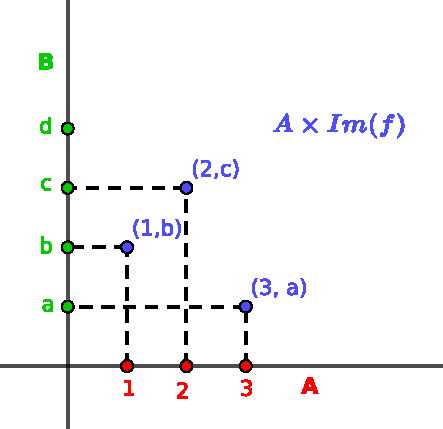
\includegraphics[width=7cm]{../Topicos/Figuras/Grf.pdf}}
    \caption{Gráfico da função $f$}
  \end{figure}

\end{exem}


\subsection{Propriedades}
As funções são classificadas em:

\begin{itemize}
 \item \textbf{Injetora}

 Uma função $f: A \rightarrow B$ é injetiva, ou injetora quando:
 \[ x_1 \neq x_2 \in A \Rightarrow f(x_1) \neq f(x_2) \in B ,\]
 ou equivalentemente usando a contrapositiva:
 \[f(x_1) = f(x_2) \in B \Rightarrow x_1 = x_2 .\]
 Ou seja, quando cada elemento da $Im(f)$ recebe um único elemento de $A= Dom(f)$, neste caso pode ocorrer de alguns elementos de $B$ não serem imagem de nenhum elemento de $A$ pela função $f$.

 \item \textbf{Sobrejetora}

 Uma função $f: A \rightarrow B$ é sobrejetiva, ou sobrejetora quando para todo $y \in B$, existe pelo menos um elemento $x \in A$ tal que $f(x) = y$. Equivalentemente em símbolos:
 $$\forall y \in B, \exists x \in A \text{ tal que } f(x) = y$$
 Ou ainda, quando cada elemento de $B$ recebe algum elemento de $A$, neste caso podendo não ser único.

 \item \textbf{Bijetora}

 Uma função $f: A \rightarrow B$ é bijetora, ou bijetiva quando for simultaneamente injetora e sobrejetora. Neste caso, $f$ admite uma inversa que é denotada por $f^{(-1)}$.

\end{itemize}

\begin{multicols}{2}
 \begin{tikzpicture}
 \node (1) at (0,0) {1};%\filldraw(1.east) circle (1pt)
 \node (2) [below of=1] {2};%\filldraw(2.east) circle (1pt)
 \node (3) [below of=2] {3};%\filldraw(3.east) circle (1pt)
 \node[fit=(1) (2) (3),ellipse,draw=red,minimum width=1cm,thick,label=below:\(A\)]{};

 \node (a) at (3,0) {a};%\filldraw($b_1$.west) circle (1pt)
 \node (b) [below of=a] {b};%\filldraw($b_2$.west) circle (1pt)
 \node (c) [below of=b] {c};%\filldraw($b_3$.west) circle (1pt)
 \node[fit=(a) (b) (c),ellipse,draw=green,minimum width=1cm,thick,label=below:\(B\)]{};

 \draw[->, shorten >=.1cm, >=stealth'] (1.east) to (c.west);
 \draw[->, shorten >=.1cm, >=stealth'] (2.east) to (b.west);
 \draw[->, shorten >=.1cm, >=stealth'] (3.east) to (a.west);
\end{tikzpicture} \\
 \textbf{bijetora}\\
 \begin{tikzpicture}
 \node (1) at (0,0) {1};%\filldraw(1.east) circle (1pt)
 \node (2) [below of=1] {2};%\filldraw(2.east) circle (1pt)
 \node (3) [below of=2] {3};%\filldraw(3.east) circle (1pt)
 \node[fit=(1) (2) (3),ellipse,draw=red,minimum width=1cm,thick,label=below:\(A\)]{};

 \node (a) at (3,0) {a};%\filldraw($b_1$.west) circle (1pt)
 \node (b) [below of=a] {b};%\filldraw($b_2$.west) circle (1pt)
 \node[fit=(a) (b),ellipse,draw=green,minimum width=1cm,thick,label=below:\(B\)]{};

 \draw[->, shorten >=.1cm, >=stealth'] (1.east) to (a.west);
 \draw[->, shorten >=.1cm, >=stealth'] (2.east) to (a.west);
 \draw[->, shorten >=.1cm, >=stealth'] (3.east) to (b.west);
\end{tikzpicture} \\
\textbf{sobrejetora e não injetora}
\end{multicols}

\begin{multicols}{2}
 \begin{tikzpicture}
 \node (1) at (0,0) {1};%\filldraw(1.east) circle (1pt)
 \node (2) [below of=1] {2};%\filldraw(2.east) circle (1pt)
 \node (3) [below of=2] {3};%\filldraw(3.east) circle (1pt)
 \node[fit=(1) (2) (3),ellipse,draw=red,minimum width=1cm,thick,label=below:\(A\)]{};

 \node (a) at (3,0) {a};%\filldraw($b_1$.west) circle (1pt)
 \node (b) [below of=a] {b};%\filldraw($b_2$.west) circle (1pt)
 \node (c) [below of=b] {c};%\filldraw($b_3$.west) circle (1pt)
 \node[fit=(a) (b) (c),ellipse,draw=green,minimum width=1cm,thick,label=below:\(B\)]{};

 \draw[->, shorten >=.1cm, >=stealth'] (1.east) to (b.west);
 \draw[->, shorten >=.1cm, >=stealth'] (2.east) to (b.west);
 \draw[->, shorten >=.1cm, >=stealth'] (3.east) to (a.west);
\end{tikzpicture} \\
\textbf{não sobrejetora e não injetora}\\
 \begin{tikzpicture}
 \node (1) at (0,0) {1};%\filldraw(1.east) circle (1pt)
 \node (2) [below of=1] {2};%\filldraw(2.east) circle (1pt)
 \node (3) [below of=2] {3};%\filldraw(3.east) circle (1pt)
 \node[fit=(1) (2) (3),ellipse,draw=red,minimum width=1cm,thick,label=below:\(A\)]{};

 \node (a) at (3,0) {a};%\filldraw($b_1$.west) circle (1pt)
 \node (b) [below of=a] {b};%\filldraw($b_2$.west) circle (1pt)
 \node (c) [below of=b] {c};%\filldraw($b_3$.west) circle (1pt)
 \node (d) [below of=c] {d};%\filldraw($b_3$.west) circle (1pt)
 \node[fit=(a) (b) (c) (d),ellipse,draw=green,minimum width=1cm,thick,label=below:\(B\)]{};

 \draw[->, shorten >=.1cm, >=stealth'] (1.east) to (b.west);
 \draw[->, shorten >=.1cm, >=stealth'] (2.east) to (c.west);
 \draw[->, shorten >=.1cm, >=stealth'] (3.east) to (a.west);
\end{tikzpicture} \\
\textbf{não sobrejetora e injetora}
\end{multicols}

\begin{exem}

 \begin{enumerate}
  \item $f: \mathbb{R} \rightarrow \mathbb{R}$ tal que $f(x) = x^2$

  Neste caso, $f$ não é sobrejetora, nem injetora.

  \begin{dem}

   \begin{itemize}
    \item Sobrejetora

    $f$ não é sobrejetora porque $x^2 \geq 0$, $\forall x \in \mathbb{R}$, logo se considerarmos $y < 0 \in \mathbb{R}$ teremos que $\nexists x \in \mathbb{R}$ tal que $f(x)= y$. Portanto $f$ não é sobrejetora.
    \fim
    \item Injetora

     Note que $ \forall x \in \mathbb{R} \Rightarrow -x \in \mathbb{R}$ e que
    \[f(-x)= (-x)^2 = (-x)*(-x) = (x)*(x) = x^2 = f(x)\]
    o que mostra que $f$ não é injetora.

   \end{itemize}
  \end{dem}

  \item $f: \mathbb{R_{+}} \rightarrow \mathbb{R}$ tal que $f(x) = x^2$

  Neste caso, $f$ não é sobrejetora, mas é injetora.

  \begin{dem}
   \begin{itemize}
    \item Sobrejetora

    $f$ não é sobrejetora porque $x^2 \geq 0$, $\forall x \in \mathbb{R}$, logo se considerarmos $y < 0 \in \mathbb{R}$ teremos que $\nexists x \in \mathbb{R}$ tal que $f(x)= y$. Portanto $f$ não é sobrejetora.
    \fim
    \item Injetora

    Tome $x_1=x_2 \in \mathbb{R_{+}}$ qualquer, como
    \[x_1=x_2 \Rightarrow x_1^2=x_2^2 \Rightarrow f(x_1)=f(x_2)\]
    logo $f$ é injetora.

   \end{itemize}
  \end{dem}

  \item $f: \mathbb{R} \rightarrow \mathbb{R_{+}}$ tal que $f(x) = x^2$

  Neste caso, $f$ é sobrejetora, mas não é injetora.

  \begin{dem}
   \begin{itemize}
    \item Sobrejetora

    Tome $y \in \mathbb{R_{+}}$ qualquer, como $y \geq 0$ existe $x \in \mathbb{R}$ tal que
    \[x = \sqrt{y} \Rightarrow x^2 = (\sqrt{y})^2 \Rightarrow x^2 = y \Rightarrow f(x) = y \]
    portanto $f$ é sobrejetora.
    \fim
    \item Injetora

    Note que $ \forall x \in \mathbb{R} \Rightarrow -x \in \mathbb{R}$ e que
    \[f(-x)= (-x)^2 = (-x)*(-x) = (x)*(x) = x^2 = f(x)\]
    o que mostra que $f$ não é injetora.

   \end{itemize}
  \end{dem}

  \item $f: \mathbb{R_{+}} \rightarrow \mathbb{R_{+}}$ tal que $f(x) = x^2$ ou $f: \mathbb{R_{-}} \rightarrow \mathbb{R_{+}}$ tal que $f(x) = x^2$

  Neste caso, $f$ é sobrejetora, e é injetora, portanto bijetora.

  \begin{dem}
   \begin{itemize}
    \item Sobrejetora

    Tome $y \in \mathbb{R_{+}}$ qualquer, como $y \geq 0$ existe $x \in \mathbb{R}$ tal que
    \[x = \sqrt{y} \Rightarrow x^2 = (\sqrt{y})^2 \Rightarrow x^2 = y \Rightarrow f(x) = y\]
    portanto $f$ é sobrejetora.
    \fim
    \item Injetora

    Tome $x_1, x_2 \in \R_{+}$, tais que $f(x_1) = f(x_2)$ logo,
    \[f(x_1) = f(x_2) \Rightarrow x_1^2= x_2^2 \Rightarrow \sqrt{x_1^2}= \sqrt{x_2^2} \Rightarrow |x_1|= |x_2| \Rightarrow x_1= x_2, \]
    pois $x_1, x_2 \geqslant 0$. Portanto $f$ é injetora.

   \end{itemize}
  \end{dem}

 \end{enumerate}

\end{exem}

\subsection{Operações com funções}
Dadas as funções $f: A \rightarrow \R$, $g: B \rightarrow \R$, se $A \cap B \neq \emptyset$, então $\forall x \in A \cap B$, definimos as seguintes operações entre estas funções:
\[(f + g)(x)= f(x) + g(x); \]
\[(f - g)(x)= f(x) - g(x); \]
\[(f \cdot g)(x)= f(x) \cdot g(x); \]
\[ \left( \frac{f}{g} \right) (x)= \frac{f(x)}{g(x)} ;\]
\[(k \cdot f)(x)= k \cdot f(x), \text{ para } k \text{ constante} ,\]

note que:
\[dom(f+g)= dom(f-g)= dom(f \cdot g)= dom(k \cdot f)= A \cap B ,\]
\[ dom\left( \frac{f}{g} \right)= \{x \in A \cap B \mid g(x) \neq 0\}. \]

Além destas operações, é possível também definir a composição de funções. Para isso consideremos duas funções $f: A \rightarrow B$ e $g: C \rightarrow D$, com $A, B, C \text{ e } D \subset \R$, e tais que $Im(f) \subset C$ , assim a função composta $g \circ f: A \rightarrow D$ é definida por:
\[(g \circ f)(x)= g(f(x)). \]

\section{Tipos de funções}

\subsection{Função constante}

É a função que associa todos os elementos do domínio a um único elemento do contradomínio. Ou seja, dado $a \in \R$ fixo, a função $f$:
\begin{eqnarray*}
 f: \R & \rightarrow & \R \\
 x & \mapsto & a,
\end{eqnarray*}
é uma função constante.

Por exemplo, a função $f$:
\begin{eqnarray*}
 f: \R & \rightarrow & \R \\
 x & \mapsto & 2 \ .
\end{eqnarray*}

É uma função constante. Para construir o gráfico desta função começamos encontrando alguns pontos $(x, y)= (x, f(x))$ do gráfico, o que pode ser feito através da seguinte tabela:

 \begin{table}[H]
 \centering
 \begin{tabular}{|c|c|c|} \hline
 \rowcolor{cinza}
  x & f(x)= 2 & (x, y)  \\\hline
  -1 & f(-1)= 2 & (-1, 2) \\\hline
   0 & f(0)= 2 & (0, 2)  \\\hline
   1 & f(1)= 2 & (1, 2) \\\hline
 \end{tabular}
\end{table}

Após encontrar os pontos basta marcar os mesmo o plano cartesiano e traçar a curva que liga estes pontos com isso objetos o gráfico da função. Neste caso o gráfico é:
\begin{figure}[H]
 \centering
    \fbox{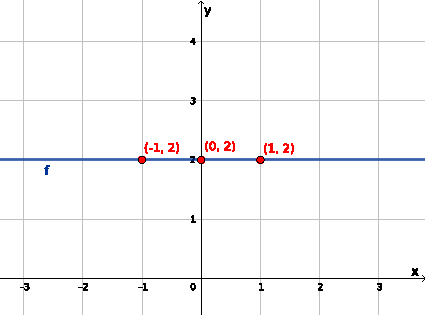
\includegraphics[width=7cm]{../Topicos/Figuras/f(x)=2.pdf}}
    \caption{Gráfico da função $f(x)=2$}
  \end{figure}

\subsection{Função identidade}

A função $Id$:
\begin{eqnarray*}
 Id: \R & \rightarrow & \R \\
 x & \mapsto & x \ ,
\end{eqnarray*}
é chamada \textit{função identidade real}.

Para encontrar alguns pontos $(x, f(x))$ do gráfico desta função, construímos a seguinte tabela:

 \begin{table}[H]
 \centering
 \begin{tabular}{|c|c|c|} \hline
 \rowcolor{cinza}
  x & f(x)= x & (x, y)  \\\hline
  -1 & f(-1)= -1 & (-1, -1) \\\hline
   0 & f(0)= 0 & (0, 0)  \\\hline
   1 & f(1)= 1 & (1, 1) \\\hline
 \end{tabular}
\end{table}

Logo o gráfico da função $Id$ é:
\begin{figure}[H]
 \centering
    \fbox{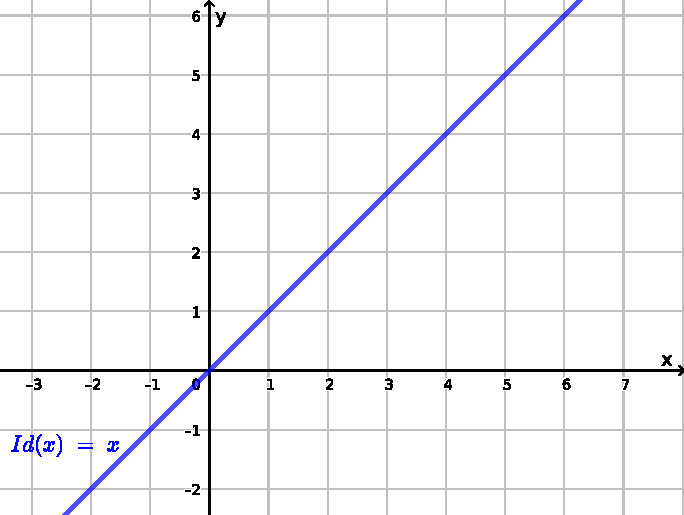
\includegraphics[width=7cm]{../Topicos/Figuras/Id(x)=x.pdf}}
    \caption{Gráfico da função $Id(x)=x$}
  \end{figure}


\subsection{Funções polinomiais de grau \texorpdfstring{$n$}{n}}

 \vskip0.3cm
 \colorbox{azul}{
 \begin{minipage}{0.9\linewidth}
 \begin{center}
 As funções $f: \R \to \R$ com a seguinte regra geral:
 \[f(x) = a_0 + a_1 x + a_2 x^2 + a_3 x^3 + \cdots + a_n x^n\]
 para $\{a_0, a_1, a_2, a_3, \ldots a_n\} \in \R$ e $n \in \N$, tais que $a_n \neq 0$ são denominadas \\ \textbf{funções polinomiais de grau $n$}.
 \end{center}
 \end{minipage}}
 \vskip0.3cm

 

 Casos particulares:
 \begin{itemize}
 \item Funções do 1º grau, ou funções afim

 São funções $f: \R \rightarrow \R$ dadas por:
 \[f(x)= ax + b \ , \]

 para certos $a, b \in \R$ com $a \neq 0$. Note que um caso particular e já conhecido de função de 1º grau é a função identidade, $f(x)= x$, a qual possui $a=1$ e $b=0$. 
 
 Vejamos mais alguns exemplos de funções de 1º grau.
 
 Consideremos as funções $f, g: \R \to \R$ dadas por:
 \begin{enumerate}[a)]
  \item $f(x)= x+2$
  \item $g(x)= x-1$
 \end{enumerate}

 
 \begin{figure}[H]
   \fbox{\subfigure[$f(x)= x+2$]{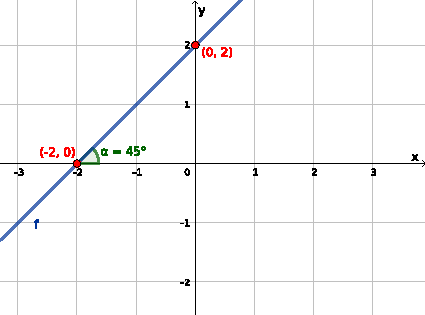
\includegraphics[width=7cm,height=6cm]{../Topicos/Figuras/f(x)=x+2.pdf}}}
   \fbox{\subfigure[$g(x)= x-1$]{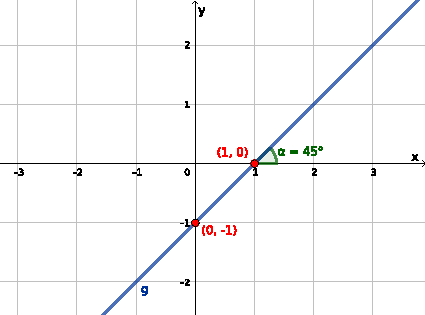
\includegraphics[width=7cm,height=6cm]{../Topicos/Figuras/f(x)=x-1.pdf}}}
  \end{figure} 
  Note que o que muda na definição destas funções é apenas o coeficiente $b$. Fazendo uma análise comparativa dos gráficos destas funções notamos que os ângulos que as retas formam com o eixo $x$ é o mesmo, portanto as retas são paralelas, porém o ponto de interseção das retas com o eixo $y$, que são os pontos $(0, f(0))$, $(0, g(0))$ muda, ou seja, $f(0) \neq g(0)$. De fato:
  \[f(0)= 0 + 2= 2\]
  \[g(0)= 0 -1 = -1 \ .\]
  No caso geral em que $f(x)=ax+b$, teremos que $f(0)=a0 + b= b$, portanto o gráfico de $f$ irá intersectar o eixo $y$ no ponto $(0,b)$. O coeficiente $b$ é chamado de \textbf{coeficiente linear} da reta/função linear.
  
  Consideremos as funções $f, g: \R \to \R$ dadas por:
 \begin{enumerate}[a)]
  \item $f(x)= 2x$
  \item $g(x)= -2x$
 \end{enumerate}
  
 \begin{figure}[H]
   \fbox{\subfigure[$f(x)= 2x$]{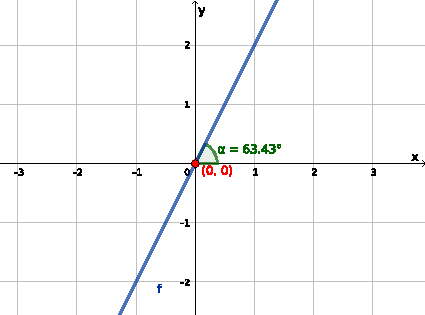
\includegraphics[width=7cm,height=6cm]{../Topicos/Figuras/f(x)=2x.pdf}}}
   \fbox{\subfigure[$g(x)= -2x$]{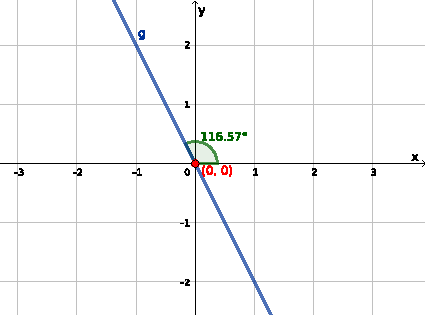
\includegraphics[width=7cm,height=6cm]{../Topicos/Figuras/g(x)=-2x.pdf}}}
  \end{figure} 
  Neste exemplos estamos mudando apenas o coeficiente $a$ das funções, o que está alterando o ângulo que as retas formam com o eixo $x$, ou seja a inclinação das retas em relação ao eixo $x$. Já o ponto de interseção das retas com o eixo $y$ é o mesmo pois $f(0)= g(0)= 0$. O coeficiente $a$ é chamado de \textbf{coeficiente angular} da reta/função linear.
  
   \vskip0.3cm
 \colorbox{amarelo}{
 \begin{minipage}{0.9\linewidth}
 \begin{center}
 O gráfico de uma função linear $f: \R \to \R$ dada por:
 \[f(x) = ax + b\]
 é uma reta com coeficiente angular $a$ e cuja interseção com o eixo $y$ ocorre no ponto $(0, b)$.
 \end{center}
 \end{minipage}}
 \vskip0.3cm
 
 Frequentemente a equação da reta é dada pela equação $y=mx+n$, que nada mais é do que uma função de 1º grau, basta considerar $y=f(x)$ o que fazemos no contexto de funções para trabalhar com o gráfico da função.
 
 \textbf{Coeficiente angular da reta}
 
  Dados dois pontos $P_0=(x_0, y_0)$, $P_1=(x_1, y_1)$, com $x_0 \neq x_1$, como na figura:
 
 \begin{figure}[H]
 \centering
    \fbox{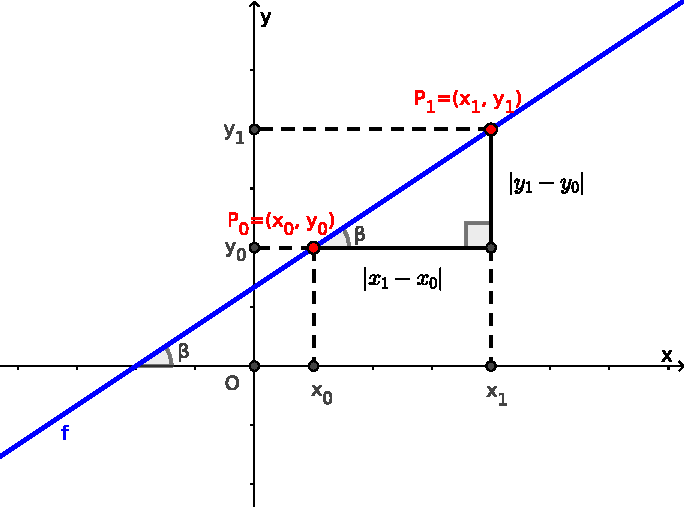
\includegraphics[width=8cm]{../Topicos/Figuras/coefangular.pdf}}
    \caption{Coeficiente angular}
  \end{figure}
  
  o coeficiente angular da reta que passa por estes dois pontos é dado por:
  \[a= \frac{y_1 - y_0}{x_1 - x_0} \ \ \ \text{ ou } \ \ \ a= \frac{y_0 - y_1}{x_0 - x_1} \ .\]
  
  De fato, dados dois pontos $P_0=(x_0, y_0)$, $P_1=(x_1, y_1)$, com $x_0 \neq x_1$, podemos encontrar a função $f(x)= ax+b$, cujo gráfico passa por estes dois pontos lembrando que ambos devem satisfazer a equação da função assim obtemos:
  \[ \begin{cases}
   y_0= ax_0 + b \\
   y_1= ax_1 + b
  \end{cases} \]
  logo $y_0 - ax_0= b$, substituindo na segunda equação decorre que:
  \[y_1= ax_1 + y_0 - ax_0 \Rightarrow y_1 - y_0= a(x_1 - x_0) \Rightarrow a= \frac{y_1 - y_0}{x_1 - x_0} \ . \]
  
  Este sistema linear sempre pode ser usado para encontrar a regra da função linear que passa por dois pontos dados.

  
  \begin{exem}
  Vamos determinar o coeficiente angular da reta que passa pelos pontos:
   \begin{enumerate}[a)]
    \item $P_0=(0,2)$ e $P_1=(-2,0)$
    \[a= \frac{y_1 - y_0}{x_1 - x_0}= \frac{0 - 2}{-2 - 0}= \frac{-2}{-2}= 1\]
    \item $P_0=(1,2)$ e $P_1=(-1,-2)$
    \[a= \frac{y_1 - y_0}{x_1 - x_0}= \frac{-2 - 2}{-1 - 1}= \frac{-4}{-2}= 2\]
   \end{enumerate}

  \end{exem}
  
  Quando dados dois pontos $P_0=(x_0, y_0)$, $P_1=(x_1, y_1)$, com $x_0 = x_1$, temos uma reta vertical, cuja equação é $x= a$ para algum $a \in \R$, que não é o gráfico de uma função, por isso não iremos detalhar este caso.
  
  Dadas duas funções lineares $f(x)=a_1 x + b_1$ e $g(x)= a_2 x + b_2$, tais que $f(x) \neq g(x)$, a partir da análise de seus coeficientes angulares podemos conhecer a posição relativa de seus gráficos. Nesta situação temos que dois casos especiais:
  \begin{itemize}
  \item Se $a_1= a_2$ então os gráficos de $f$ e $g$ são retas \textbf{paralelas};
  \item Se $a_1 \cdot a_2= -1$ então os gráficos de $f$ e $g$ são retas \textbf{perpendiculares}.
  \end{itemize}
  
  \begin{exem}
  Considere as funções $g(x)= -2x+4$, $f(x)= -2x+2$, $h(x)= \frac{-1}{-2}x+ 1,5$, pela análise com coeficientes angulares temos que os gráficos de $g$ e $f$ são retas paralelas e os gráficos $g$ e $h$ são retas perpendiculares, como podemos ver nos seguintes gráficos:
     \begin{figure}[H]
   \fbox{\subfigure[Retas paralelas]{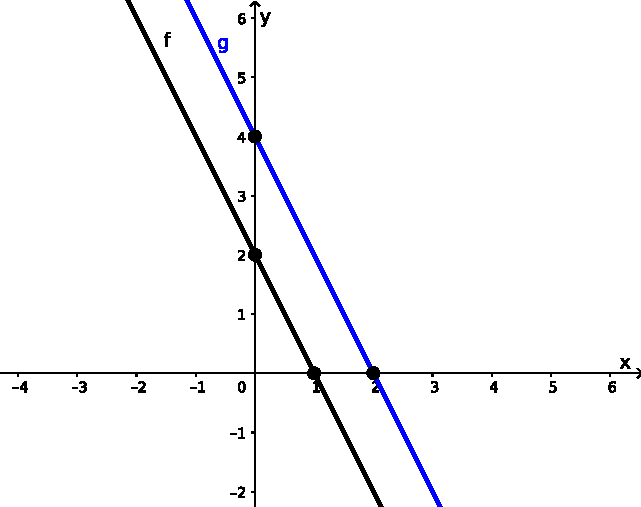
\includegraphics[width=7cm,height=6cm]{../Topicos/Figuras/retasparalelas.pdf}}}
   \fbox{\subfigure[Retas perpendiculares]{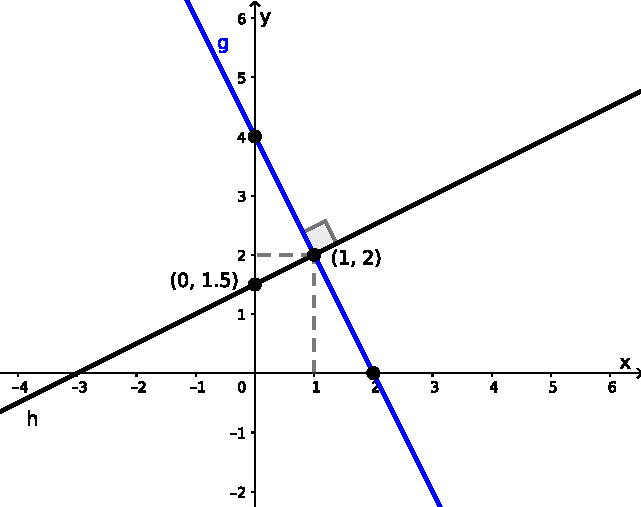
\includegraphics[width=7cm,height=6cm]{../Topicos/Figuras/retasperpendiculares.pdf}}}
  \end{figure} 
  \end{exem}

  
  
 \textbf{Zeros ou raízes das funções lineares}
 
 \vskip0.3cm
 \colorbox{azul}{
 \begin{minipage}{0.9\linewidth}
 \begin{center}
 Os zeros ou raízes de uma função $y= f(x)$ são os $x \in Dom(f)$ tais que $f(x)= 0$.
 \end{center}
 \end{minipage}}
 \vskip0.3cm
 
 Desta definição de \textbf{zeros} decorre que os zeros de uma função de 1º grau são as raízes da equação $ax+b=0$. Como esta equação é do 1º grau, ela possui uma única raiz, logo a função de 1º grau também possui uma única raiz, que denotaremos por $\tilde{x}$. Note que o ponto $(\tilde{x}, 0) \in \R^2$ é o ponto de interseção do gráfico da $f$ com o eixo $x$, assim podemos interpretar graficamente as raízes da nossa função como sendo os pontos de interseção do gráfico da função com o eixo das abscissas.

 \item Funções do 2º grau ou função quadrática

 São funções $f: \R \rightarrow \R$ dadas por:
 \[f(x)= ax^2 + bx + c\]

 Os \textbf{zeros} ou \textbf{raízes} das funções de 2º grau $f$, quando existem, são os $x \in dom(f)$ tais que $ax^2+bx+c=0$. Por ser esta uma equação do 2º grau temos três situações a considerar, dependendo do valor de $\Delta$:
 \[\destaque{\Delta= b^2 - 4*a*c}\]
 Se $\destaque{\Delta < 0}$ a função $f$ não possui raízes reais;

 Se $\destaque{\Delta = 0}$ a função $f$ possui uma única raiz real;

 Se $\destaque{\Delta > 0}$ a função $f$ possui duas raízes reais distintas, que podem ser calculadas resolvendo a equação de 2º grau através da fórmula para equações de 2º grau.
 
 Por definição, os zeros da função $f(x)= ax^2+bx+c$, são as raízes da equação $ax^2+bx+c=0$, já que estes são os valores de $x$ para os quais $f(x)=0$. Graficamente, quando estas funções possuem zeros eles são exatamente os pontos de interseção do gráfico da $f$ com o eixo $x$.

 Com relação a concavidade, o gráfico da função de 2º grau tem concavidade voltada \textbf{para cima} quando $\destaque{a > 0}$, e concavidade voltada \textbf{para baixo} quando $\destaque{a < 0}$.

 Em ambos os casos a função do 2º grau possui um vértice dado pela seguinte equação:

 \[ \destaque{V= \left(\frac{- b}{2a}, \frac{- \Delta}{4a} \right)} .\]

 No caso em que $a > 0$, o vértice do gráfico da função de 2º grau é um ponto de mínimo da função.

 No caso em que $a < 0$, o vértice do gráfico da função de 2º grau é um ponto de máximo da função.


  \begin{figure}[H]
   \fbox{\subfigure[$a > 0$ e $\Delta < 0$]{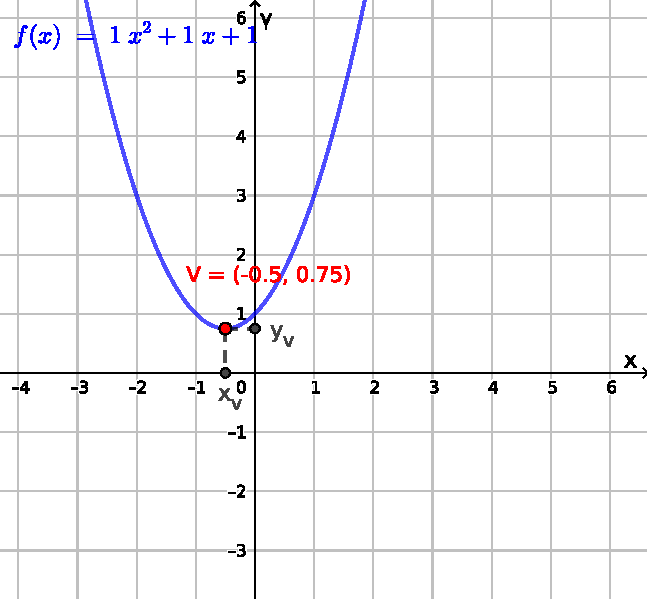
\includegraphics[width=7cm,height=6cm]{../Topicos/Figuras/f1.pdf}}}
   \fbox{\subfigure[$a > 0$ e $\Delta = 0$]{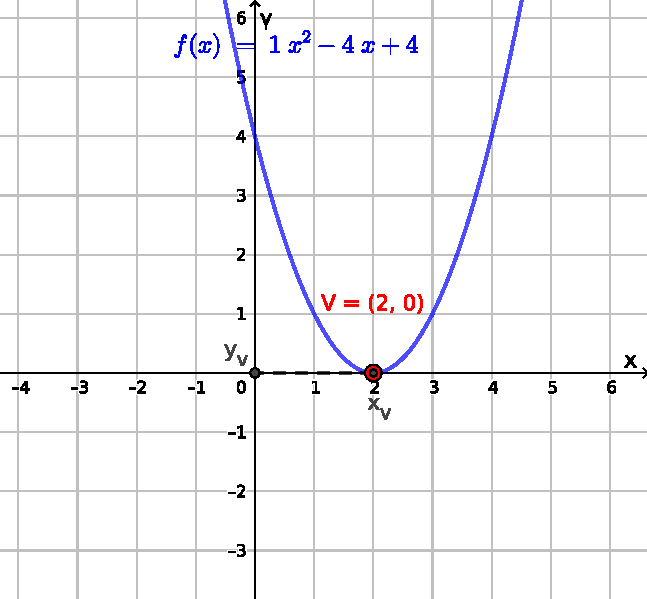
\includegraphics[width=7cm,height=6cm]{../Topicos/Figuras/f2.pdf}}}
  \end{figure} 
  
  \begin{figure}[H] 
   \fbox{\subfigure[$a > 0$ e $\Delta > 0$]{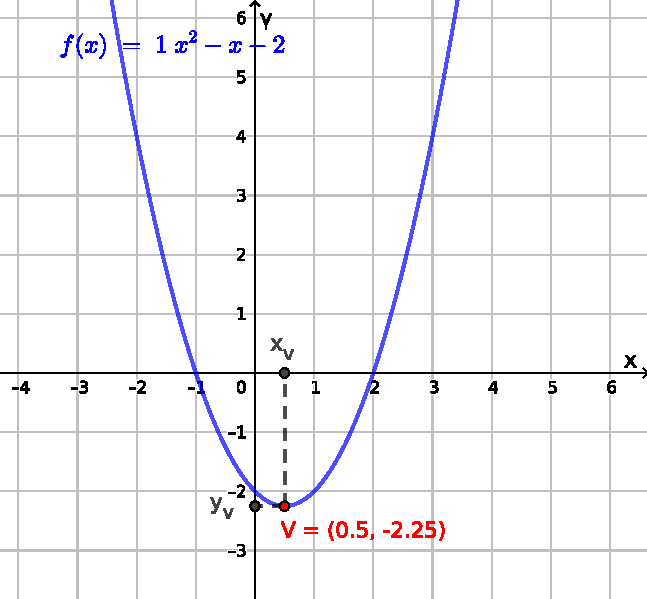
\includegraphics[width=7cm,height=6cm]{../Topicos/Figuras/f3.pdf}}}
   \fbox{\subfigure[$a < 0$ e $\Delta < 0$]{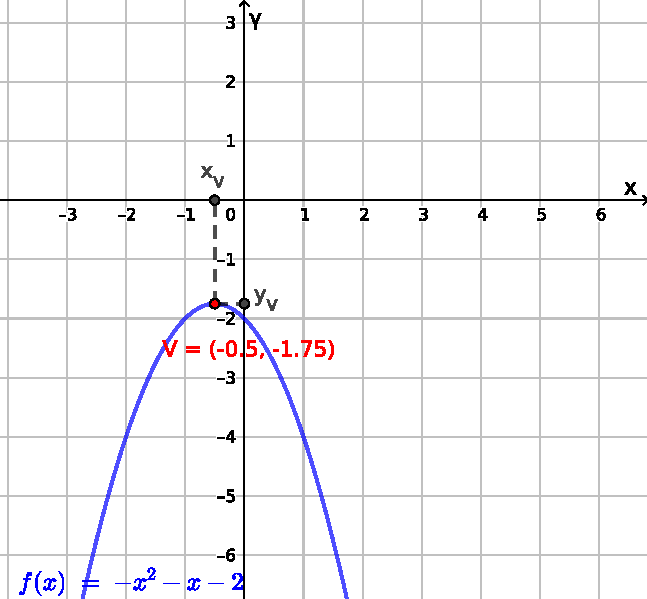
\includegraphics[width=7cm,height=6cm]{../Topicos/Figuras/f4.pdf}}}
  \end{figure}
  
   \begin{figure}[H]
   \fbox{\subfigure[$a < 0$ e $\Delta = 0$]{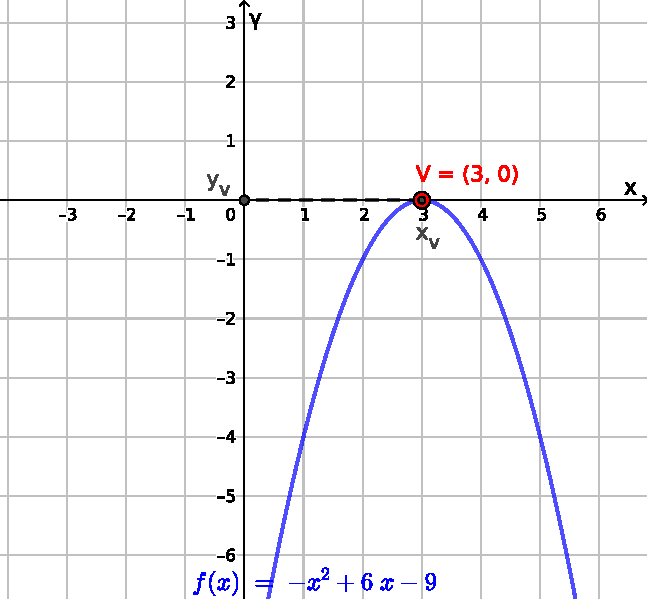
\includegraphics[width=7cm,height=6cm]{../Topicos/Figuras/f5.pdf}}}
   \fbox{\subfigure[$a < 0$ e $\Delta > 0$]{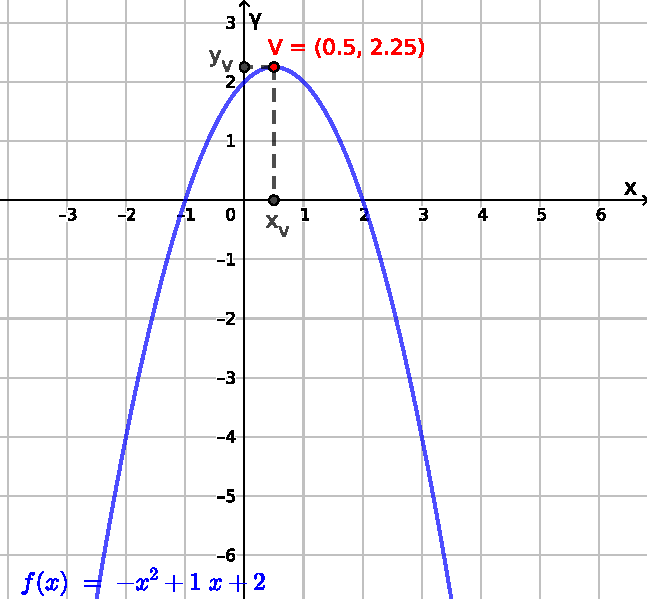
\includegraphics[width=7cm,height=6cm]{../Topicos/Figuras/f6.pdf}}}
   \caption{Gráficos de funções do 2º grau}
 \end{figure}


 \newpage
 \item Funções do 3º grau ou funções cúbicas

 São funções $f: \R \rightarrow \R$ dadas por:
 \[f(x)= ax^3 + bx^2 + cx + d .\]
 
 As \textbf{raízes} ou \textbf{zeros} das funções de 3º grau são os $x \in \R$ tais que $ax^3 + bx^2 + cx + d=0$. Assim as funções de 3º grau podem classificadas de acordo com suas raízes em 4 casos:
 \begin{enumerate}[(I)]
  \item 3 raízes reais distintas;
  \item 1 raiz real e duas raízes complexas;
  \item 3 raízes reais sendo duas delas iguais;
  \item 3 raízes reais iguais.
 \end{enumerate}
 Estes casos estão representados nos gráficos abaixo, onde consideramos sempre $a< 0$, o caso $a> 0$ é análogo.


   \begin{figure}[H]
   \fbox{\subfigure[$a < 0$]{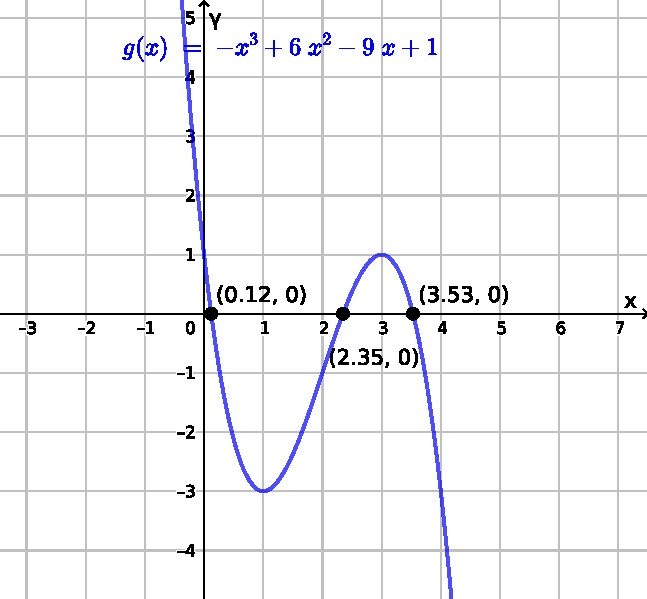
\includegraphics[width=7cm,height=5cm]{../Topicos/Figuras/g1.pdf}}}
   \fbox{\subfigure[$a < 0$]{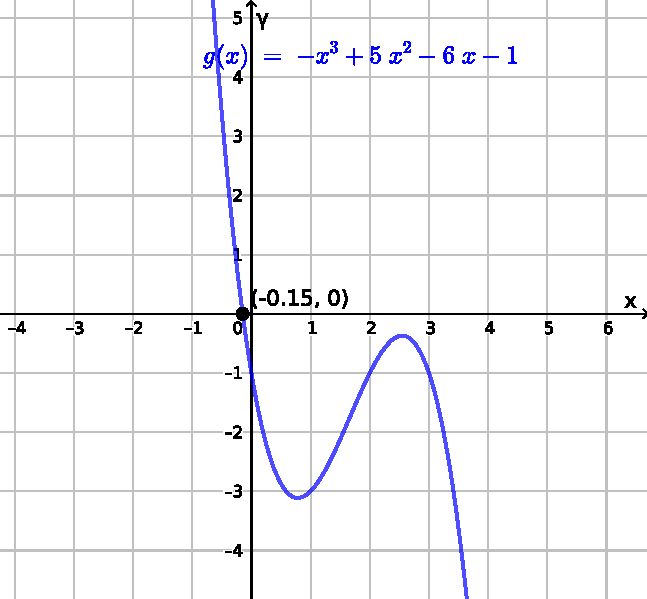
\includegraphics[width=7cm,height=5cm]{../Topicos/Figuras/g2.pdf}}}
   \end{figure}
   
  \begin{figure}[H]
   \fbox{\subfigure[$a < 0$]{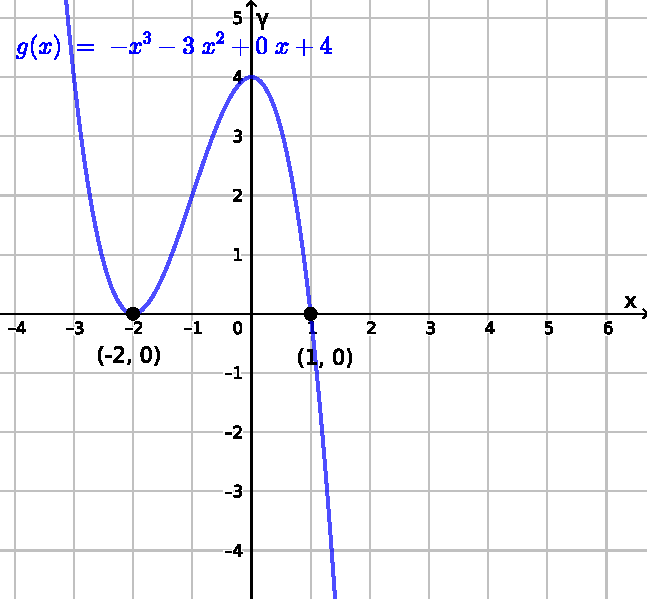
\includegraphics[width=7cm,height=5cm]{../Topicos/Figuras/g3.pdf}}}
   \fbox{\subfigure[$a < 0$]{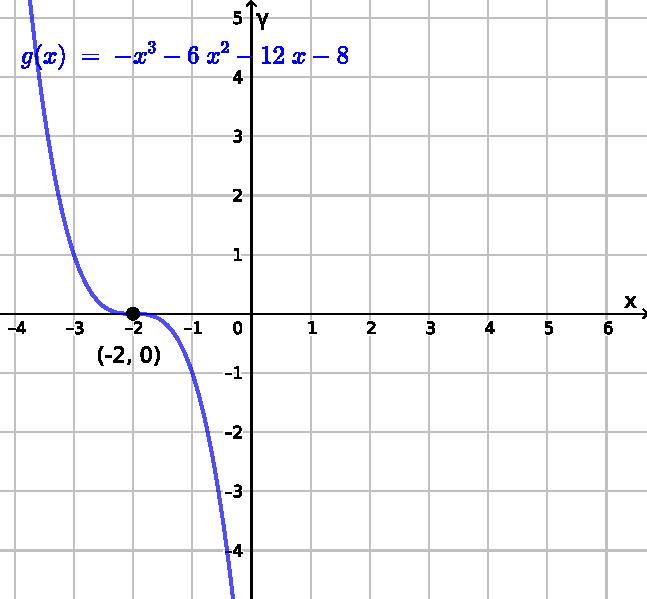
\includegraphics[width=7cm,height=5cm]{../Topicos/Figuras/g4.pdf}}}
   \caption{Gráficos de funções do 3º grau}
  \end{figure}
 
 \end{itemize}
 

  \subsection{Função modular}
  
  Considere a função $f: \R \rightarrow \R$, dada por $f(x)= |x|$, pela definição de módulo temos que $f$ é uma função definida por partes, da seguinte forma:

  \[f(x)= |x| = \begin{cases}
                 x, \text{ se } x \geq 0 \\
                 -x, \text{ se } x < 0
                \end{cases} \ .\]
 
 Cujo gráfico é dado por:
                
  \begin{figure}[H]
 \centering
    \fbox{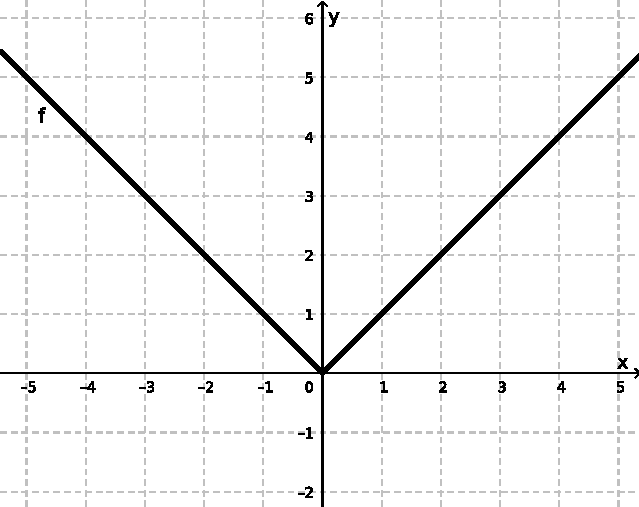
\includegraphics[width=8cm]{../Topicos/Figuras/funcaomodulo.pdf}}
    \caption{Gráfico da função módulo}
  \end{figure}
  
  Note que $f$ é decrescente no intervalo $]-\infty, 0[$, e decrescente no intervalo $]0, \infty[$, e admite um mínimo em $x=0$.
  
  Consideramos agora a função $f_1: \R \rightarrow \R$ dada por $f_1(x)= |x+1|$, observe que:
  \[x+1 \geq 0 \Leftrightarrow  x \geq -1\]
  com isso podemos reescrever a função $f_1$ sem os módulos da seguinte forma:
  
  \[f_1(x)= \begin{cases}
                 x + 1, \text{ se } x \geq -1 \\
                 -x - 1, \text{ se } x < -1
                \end{cases} \ .\]
  Com isso a função modular pode ser vista como uma função linear por partes.
  
  Analogamente, para a função $f_2: \R \rightarrow \R$ dada por $f_2(x)= |x+1|+2$, temos que:
  \[x+1 \geq 0 \Leftrightarrow  x \geq -1\]
  com isso podemos reescrever a função $f_2$ sem os módulos da seguinte forma:
  
  \[f_2(x)= \begin{cases}
                 x + 3, \text{ se } x \geq -1 \\
                 -x + 1, \text{ se } x < -1
                \end{cases} \ .\]
  Com isso a função modular também pode ser vista como uma função linear por partes.
  
  Os gráficos das funções $f$, $f_1$ e $f_2$ estão dados na figura a seguir.  
  
  \begin{figure}[H]
 \centering
    \fbox{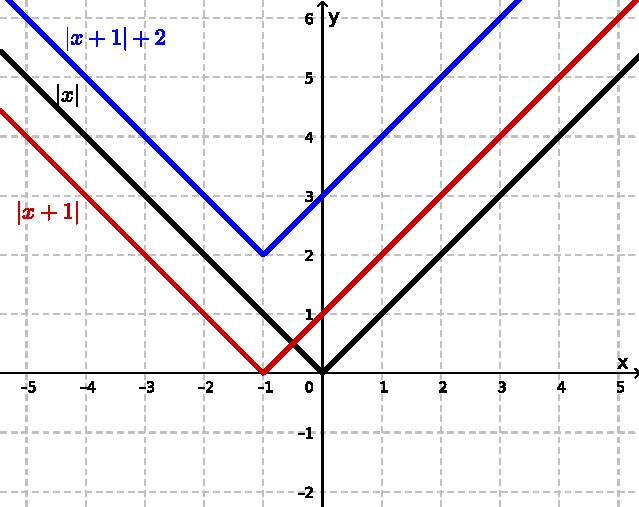
\includegraphics[width=8cm]{../Topicos/Figuras/funcaomodulo2.pdf}}
    \caption{Gráfico da função módulo}
  \end{figure}
  
  Comparando os gráficos das funções $f$ e $f_1$ notamos que ao somar uma constante "dentro" do módulo transladamos o gráfico da função $f$ no eixo $x$, e ao comparar as funções $f_1$ e $f_2$ percebemos que ao somar uma constante "fora" do módulo fazemos uma translação do gráfico da função $f_1$ em relação ao eixo $y$.
  
  \subsection{Mais algumas funções interessantes}
  
  \textbf{Função raíz quadrada}
  
  É a função $f: \R_{+} \to \R_{+}$ dada por $f(x)= \sqrt{x}$, cujo gráfico é:
  
   \begin{figure}[H]
 \centering
    \fbox{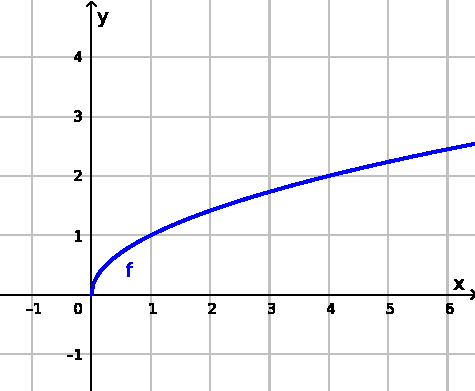
\includegraphics[width=6cm]{../Topicos/Figuras/funcaoraizquadrada.pdf}}
    \caption{Função raíz quadrada}
  \end{figure}
  
  Note que neste caso o domínio da função são apenas os números reais positivos, já que não existe raíz quadrada de número negativo.
  
  \newpage
  \textbf{Função raíz cúbica}
  
  É a função $f: \R \to \R$ dada por $f(x)= \sqrt[3]{x}$, cujo gráfico é:
  
   \begin{figure}[H]
 \centering
    \fbox{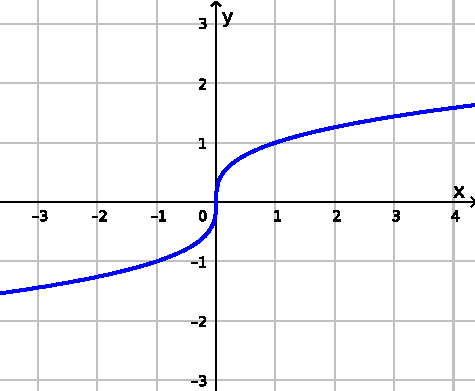
\includegraphics[width=6cm]{../Topicos/Figuras/funcaoraizcubica.pdf}}
    \caption{Função raíz cúbica}
  \end{figure} 
  
  \textbf{Função recíproca}
  
  É a função $f: \R \setminus \{0\} \to \R$ dada por $f(x)= \frac{1}{x}$, cujo gráfico é:
  
   \begin{figure}[H]
 \centering
    \fbox{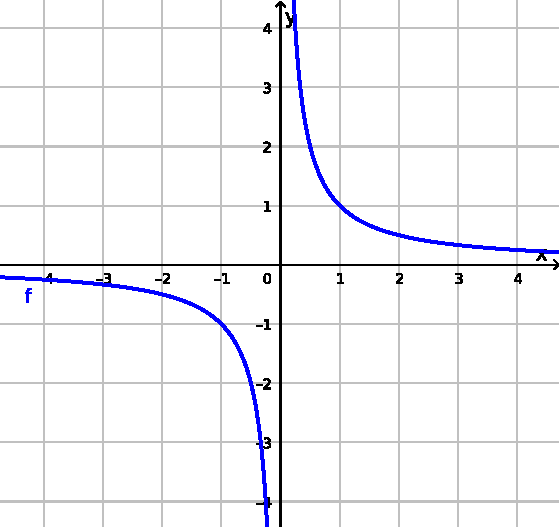
\includegraphics[width=6cm]{../Topicos/Figuras/funcaoreciproca.pdf}}
    \caption{Função recíproca}
  \end{figure}
  
  Neste caso o domínio da função é o conjunto $\R \setminus \{0\}$, pois não existe divisão por $0$ (zero).
  
  \newpage

  \textbf{Função floor}
  
  É a função $f: \R \to \R$ dada por $f(x)= \lfloor {x} \rfloor$, cujo gráfico é:
  
   \begin{figure}[H]
 \centering
    \fbox{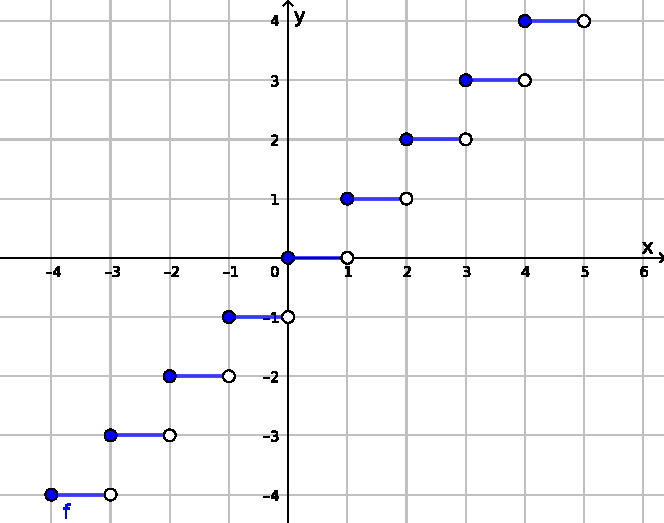
\includegraphics[width=6cm]{../Topicos/Figuras/funcaofloor.pdf}}
    \caption{Função floor}
  \end{figure}
  
  Esta função aplicada em um número $x$ tem como imagem a parte inteira do número $x$.
  
  \textbf{Função ceil}
  
  É a função $f: \R \to \R$ dada por $f(x)= \lceil {x} \rceil$, cujo gráfico é:
  
   \begin{figure}[H]
 \centering
    \fbox{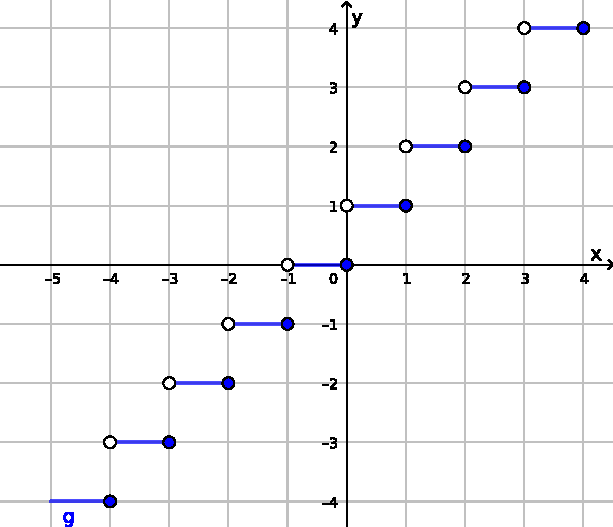
\includegraphics[width=6cm]{../Topicos/Figuras/funcaoceil.pdf}}
    \caption{Função ceil}
  \end{figure}
  
  Esta função aplicada em um número $x$ tem como imagem o menor inteiro maior ou igual a $x$.
  
  \section{Algumas propriedades das funções}
  
   \vskip0.3cm
 \colorbox{azul}{
 \begin{minipage}{0.9\linewidth}
 \begin{center}
  Dados $A, B \subset \R$ e uma função $f: A \rightarrow B$. 
  
  Dizemos que $f$ é uma \textbf{função crescente} em um intervalo $I \subset A$ se, para todo $x, y \in I$,
  \[ x < y \Rightarrow f(x) < f(y) \ .\]
  Dizemos que $f$ é uma \textbf{função descrescente} em um intervalo $I \subset A$ se, para todo $x, y \in I$,
  \[x < y \Rightarrow f(x) > f(y) \ .\]
  Dizemos que $f$ é uma \textbf{função constante} em um intervalo $I \subset A$ se, para todo $x, y \in I$,
  \[x \neq y \Rightarrow f(x) = f(y) \ .\]
 \end{center}
 \end{minipage}}
 \vskip0.3cm
 
 \begin{exem}
 Seja $f: \R \to \R$ uma função dada por $f(x)= ax + b$.
 
 Quando $\destaque{a > 0}$, dados $x_1 < x_2 \in dom(f)$, temos que:
 \[x_1 < x_2 \Rightarrow ax_1 < ax_2 \Rightarrow ax_1 + b < ax_2 + b \ ,\]
  portanto $f(x_1) < f(x_2)$, neste caso dizemos que $f$ é \textbf{crescente}. 

 Quando $\destaque{a < 0}$, dados $x_1 < x_2 \in dom(f)$, temos que:
 \[x_1 < x_2 \Rightarrow ax_1 > ax_2 \Rightarrow ax_1 + b > ax_2 + b \ ,\]
 portanto $f(x_1) > f(x_2)$, neste caso dizemos que $f$ é \textbf{decrescente}.
 
 Observe que no caso das funções de 1º grau a propriedade de ser crescente ou decrescente é válida em todo o domínio da função, nestes casos dizemos que é uma propriedade global da função.
 \end{exem}
 
 \begin{exem}
 Vamos retomar alguns dos nossos exemplos de funções para classificar como crescente, descrescente e constante. Para isso considere $x_1= -2$ e $x_2= 1$, neste caso, $x_1 < x_2$. 
  \begin{enumerate}[a)]
   \item Sendo $f(x)= \frac{1}{2}x + 1,5$, temos que 
   \[f(x_1)= f(-2)= \frac{1}{2}\cdot (-2) + 1,5= -1 + 1,5= 0,5\]
   \[f(x_2)= f(1)= \frac{1}{2} \cdot 1+\frac{3}{2}= \frac{4}{2}= 2\]
   logo $f(x_1)= 0,5 < 2= f(x_2)$. Portanto $f$ é crescente.
   \item Sendo $f(x)= -2x + 2$, temos que
   \[f(x_1)= f(-2)= -2 \cdot (-2) + 2= 4 + 2= 6\]
   \[f(x_2)= f(1)= -2 \cdot 1 + 2= 0\]
   logo $f(x_1)= 6 > 0 = f(x_2)$. Portanto $f$ é decrescente.
   \item Sendo $f(x)= 2$, temos que 
   \[f(x_1)= f(-2)= 2\]
   \[f(x_2)= f(1)= 2\]
   logo $f(x_1)= 2 = 2= f(x_2)$. Portanto $f$ é constante.
  \end{enumerate}
  Como já mostramos acima que para as funções lineares esta propriedade é global, para fazer esta classificação é suficiente testar dois valores de $x$ como fizemos acima.

 \end{exem}
 
 \begin{exem}
  Considere a função $f(x)= |x|$. Lembramos que esta função é definida por partes, por isso faremos a análise de crescimento e decrescimento em cada uma destas partes.
  
  Caso 1: Se $x < 0$, temos que $f(x)= -x$, logo se $x_1 < x_2$,
  \[x_1 < x_2 \Rightarrow -x_1 > -x_2 \Rightarrow f(x_1) > f(x_2) \ ,\]
  por exemplo, sendo $x_1= -3$ e $x_2= -2$ temos que $x_1 < x_2$,
  \[f(x_1)= f(-3)= -(-3)= 3 > 2= -(-2)= f(-2)= f(x_2) \ .\]
  
  Portanto se $x < 0$ temos que $f$ é decrescente.
  
  Caso 2: Se $x \geq 0$, temos que $f(x)= x$, logo se $x_1 < x_2$
  \[x_1 < x_2 \Rightarrow  f(x_1) < f(x_2) \ ,\]
  por exemplo, sendo $x_1= 2$ e $x_2= 3$ temos que $x_1 < x_2$,
  \[f(x_1)= 2 > 3= f(x_2) \ .\]
  
  Portanto se $x \geq 0$ temos que $f$ é crescente.
 \end{exem}


 
 \vskip0.3cm
 \colorbox{azul}{
 \begin{minipage}{0.9\linewidth}
 \begin{center}
  Dada um função $f: \R \rightarrow \R$. 
  
  Dizemos que $f$ é uma \textbf{função par} se, para todo $x \in R$,
  \[f(-x)= f(x) \ .\]
  Dizemos que $f$ é uma \textbf{função ímpar} se, para todo $x \in R$,
  \[f(-x)= - f(x) \ .\]
 \end{center}
 \end{minipage}}
 \vskip0.3cm

 
 \begin{exem}
  \begin{enumerate}[a)]
   \item A função $f(x)= x$ é uma função ímpar;
   \[f(-x)= -x= -f(x) \]
   \item A função $f(x)= x^2$ é uma função par;
   \[f(-x)= (-x)^2= x^2 = f(x) \]
   \item A função $f(x)= x^3$ é uma função ímpar.
   \[f(-x)= (-x)^3= -x^3= -f(x)\]
  \end{enumerate}
 \end{exem}
 
 \begin{exem}
  Vamos analisar a paridade de função modular $f(x)= |x|$.
  
  Caso 1: Se $x < 0$,
  \[f(x)= |x|= -x= f(-(x))= f(-x)\]
  por exemplo, $x= -2$, neste caso,
  \[f(x)= f(-2)= |-2|= -(-2)= 2= f(2)= f(-(-2))= f(-x) \ ;\]
  
  Caso 2: Se $x \geq 0$,
  \[f(x)= |x|= x= -(-x)= |-x|= f(-x)\]
  por exemplo, $x= 2$, neste caso,
  \[f(x)= f(2)= |2|= 2= -(-2)= |-2|= f(-2)= f(-x) \ .\]
  
  Portanto $f$ é uma função par.
 \end{exem}
  
  
  \subsection{Função inversa}

 Considere uma função $f: A \rightarrow B$, para $A, B \subset \R$. Se existir uma função $g: B \rightarrow A$ tal que:
 \[(g \circ f)(x)= x, \forall x \in A \ \ \ \text {e} \ \ \
 (f \circ g)(x)= x, \forall x \in B\]
 dizemos que $f$ é inversível e que $g$ é a inversa de $f$. Denotamos por $g= f^{-1}$.
 
 Ficamos com a seguinte pergunta: Quando existe $f^{-1}$? E a resposta é:
 
 \vskip0.3cm
 
 \colorbox{azul}{
 \begin{minipage}{0.9\linewidth}
 \begin{center}
 Uma função $f: A \to B$ é inversível se, e somente se, $f$ for bijetora, ou seja, injetora e sobrejetora.
 \end{center}
 \end{minipage}}

 \vskip0.3cm

\begin{exem}
 A função $f: \R \rightarrow \R$ dada por $f(x)= x+2$ é injetora, e sobrejetora portanto, existe uma função $g: \R \rightarrow \R$ dada por $g(x)= x-2$, tal que:
 \[h(x)= (f \circ g)(x)= f(g(x))= (x-2) + 2= x-2+2= x \Rightarrow (f \circ g)(x)= Id(x)\]
 \[\text{e}\]
 \[(g \circ f)(x)= g(f(x))= (x+2) - 2= x+2-2= x \Rightarrow (g \circ f)(x)= Id(x) ,\]
 logo $g= f^{-1}$ é a função inversa de $f$.

 \begin{figure}[H]
 \centering
    \fbox{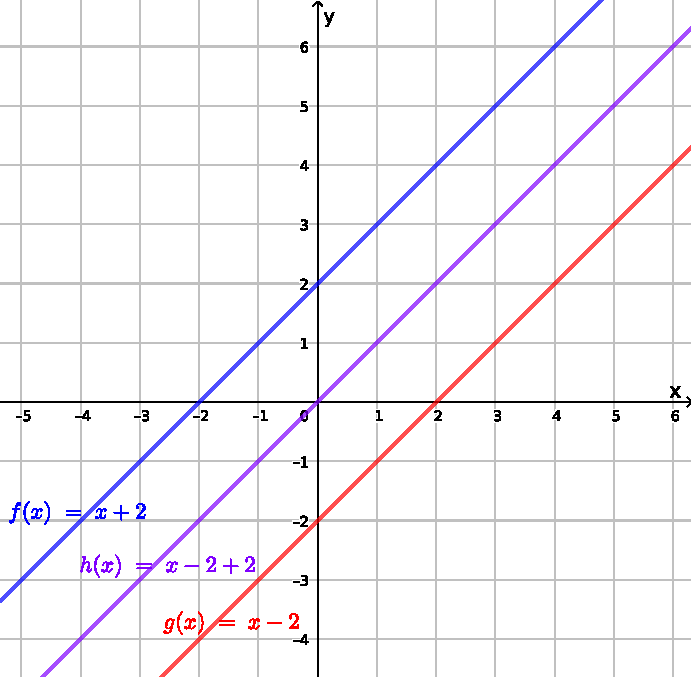
\includegraphics[width=8cm]{../Topicos/Figuras/funcao_composta.pdf}}
    \caption{Composta das funções $f$ e $g$}
  \end{figure}

\end{exem}

\newpage
 \section{Mudando os gráficos das funções}
 
 \subsection{Translação do gráfico das funções}
 
 Dados $A, B \subset \R$ e uma função $f(x): A \to B$, definimos a função translação de $f$ no eixo $y$, pela função $g(x): A \to B$, dada por \destaque{$g(x)= f(x) + c$}, onde $c \in \R$ é uma constante.
 
 \begin{exem}
  Considere a função $f(x): \R \to \R$, dada por $f(x)= x^2$. Defina as seguintes funções $g: \R \to \R$ dada por $g(x)= f(x) + 2= x^2 + 2$, e $h: \R \to \R$ dada por $h(x)= f(x) - 2= x^2 - 2$, observe na seguinte figura como estas translações alteram o gráfico da função $f$, note a função $g$ carregou o gráfico da $f$ duas unidades "para cima" no eixo $y$, já a função $h$ carregou o gráfico da $f$ duas unidades "para baixo" no eixo $y$.
  
 \begin{figure}[H]
   \fbox{\subfigure[Gráficos das funções $f$ e $g$]{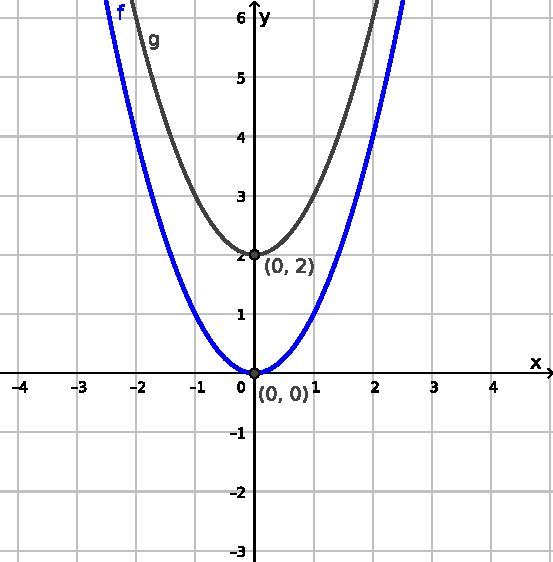
\includegraphics[width=7cm,height=6cm]{../Topicos/Figuras/translacaomais2.pdf}}}
   \fbox{\subfigure[Gráficos das funções $f$ e $h$]{\includegraphics[width=7cm,height=6cm]{../Topicos/Figuras/translacaomenos2.pdf}}}
\caption{Translação no eixo $y$}
  \end{figure}
  
 \end{exem}

  Dados $A, B \subset \R$ e uma função $f(x): A \to B$, definimos a função translação de $f$ no eixo $x$, pela função $g(x): A \to B$, dada por \destaque{$g(x)= f(x + c)$}, onde $c \in \R$ é uma constante.
 
 \begin{exem}
  Considere a função $f(x): \R \to \R$, dada por $f(x)= x^2$. Defina as seguintes funções $g: \R \to \R$ dada por $g(x)= f(x + 2)= (x+2)^2$, e $h: \R \to \R$ dada por $h(x)= f(x-2)= (x-2)^2$, observe na seguinte figura como estas translações alteram o gráfico da função $f$, note a função $g$ carregou o gráfico da $f$ duas unidades "para à esquerda" no eixo $x$, já a função $h$ carregou o gráfico da $f$ duas unidades "para à direita" no eixo $x$.
  
 \begin{figure}[H]
   \fbox{\subfigure[Gráficos das funções $f$ e $g$]{\includegraphics[width=7cm,height=6cm]{../Topicos/Figuras/translacaoXmais2.pdf}}}
   \fbox{\subfigure[Gráficos das funções $f$ e $h$]{\includegraphics[width=7cm,height=6cm]{../Topicos/Figuras/translacaoXmenos2.pdf}}}
\caption{Translação no eixo $x$}
  \end{figure}
  
 \end{exem}
 
 \subsection{Reflexão do gráfico das funções}
 
 Dados $A, B \subset \R$ e uma função $f(x): A \to B$, definimos a função reflexão de $f$ no eixo $x$, pela função $g(x): A \to B$, dada por \destaque{$g(x)= -f(x)$}.
 
 \begin{exem}
  Considere a função $f(x): \R \to \R$, dada por $f(x)= x^2$. Defina a função $g: \R \to \R$ dada por $g(x)=-f(x)= -x^2$, note que $g$ é por definição a reflexão da função $f$ em torno do eixo $x$, como pode ser visto pela figura:
  
\begin{figure}[H]
   \centering
   \fbox{\includegraphics[width=7cm]{../Topicos/Figuras/reflexaoemX.pdf}}
   \caption{Reflexão no eixo $x$}
  \end{figure}
  
 \end{exem}

 
 Dados $A, B \subset \R$ e uma função $f(x): A \to B$, definimos a função reflexão de $f$ no eixo $y$, pela função $g(x): A \to B$, dada por \destaque{$g(x)= f(-x)$}.
 
 \begin{exem}
  Considere a função $f(x): \R \to \R$, dada por $f(x)= x^3$. Defina a função $g: \R \to \R$ dada por $g(x)=f(-x)= (-x)^3$, note que $g$ é por definição a reflexão da função $f$ em torno do eixo $y$, como pode ser visto pela figura:
  
\begin{figure}[H]
   \centering
   \fbox{\includegraphics[width=7cm]{../Topicos/Figuras/reflexaoemY.pdf}}
   \caption{Reflexão no eixo $y$}
  \end{figure}
  
 \end{exem}
 
 Resumindo, dados $A, B \subset \R$, uma função $f(x): A \to B$, e uma constante $c \in \R$ obtemos as seguintes funções $g: A \to B$:
  \begin{table}[H]
 \centering
 \begin{tabular}{|c|c|} \hline
 \rowcolor{cinza}
  Mudança & Função \\\hline
  Translação no eixo $y$ & $g(x)= f(x)+ c$ \\\hline
  Translação no eixo $y$ & $g(x)= f(x)- c$ \\\hline
  Translação no eixo $x$ & $g(x)= f(x+ c)$ \\\hline
  Translação no eixo $x$ & $g(x)= f(x- c)$ \\\hline
  Reflexão no eixo $x$ & $g(x)= -f(x)$ \\\hline
  Reflexão no eixo $y$ & $g(x)= f(-x)$ \\\hline
 \end{tabular}
\end{table}
 
  \newpage
  \section{Trigonometria}

 \subsection{Triângulo retângulo}

  Considere o triângulo retângulo, (triângulo que possui um de seus ângulos internos medindo $90 \degree$), como na figura abaixo:
  \begin{figure}[H]
   \centering
   \fbox{\includegraphics[width=7cm]{../Topicos/Figuras/triangulo_retangulo.pdf}}
   \caption{Triângulo retângulo}
  \end{figure}
 para este triângulo temos que é válido o seguinte teorema:

 \vskip0.3cm

\colorbox{azul}{
 \begin{minipage}{0.9\linewidth}
 \begin{center}
 \textbf{Teorema de Pitágoras}
  \[a^2= b^2 + c^2.\]
 \end{center}
 \end{minipage}}

 \vskip0.3cm

 Este é um resultado importante, já que com ele é possível encontrar o valor de um dos lados do triângulo, nos casos em que não temos todos os lados dados.

 Para este triângulo, as funções seno, cosseno e tangente são dadas pelas seguintes razões trigonométricas, nesta ordem:

 \vskip0.3cm

\colorbox{azul}{
 \begin{minipage}{0.9\linewidth}
 \begin{center}
 \textbf{Funções trigonométricas}
  \begin{eqnarray*}
   sen(\alpha)= \frac{c}{a}= \frac{CO}{HI} \ ; \ \ cos(\alpha)= \frac{b}{a}= \frac{CA}{HI} \ ; \ \ tan(\alpha)= \frac{c}{b}= \frac{CO}{CA}.
 \end{eqnarray*}
 \end{center}
 \end{minipage}}

 \vskip0.3cm

 Como a soma dos ângulos internos de um triângulo é $180 \degree$, e estamos aqui tratando de um triângulo retângulo, decorre que neste caso $0 \degree \leqslant \alpha \leqslant 90 \degree$. Porém estas funções estão definidas para qualquer número real, mas para um primeiro estudo é suficiente conhecer seus valores para os ângulos $0 \degree \leqslant \alpha \leqslant 360 \degree$.

 Destacamos aqui os valores do seno, cosseno e tangente dos \emph{ângulos notáveis} que são os mais utilizados:

 \begin{table}[H]
 \centering
 \begin{tabular}{|c|c|c|c|c|c|} \hline
 \rowcolor{cinza}
               & $0 \degree$  & $30 \degree$  & $45 \degree$  & $60 \degree$ & $90 \degree$  \\\hline
  \textbf{sen} & $0$ &$\frac{1}{2}$ & $\frac{\sqrt{2}}{2}$ & $\frac{\sqrt{3}}{2}$ & $1$ \\\hline
  \textbf{cos} & $1$ & $\frac{\sqrt{3}}{2}$ & $\frac{\sqrt{2}}{2}$ & $\frac{1}{2}$ & $0$ \\\hline
  \textbf{tan} & $0$ & $\frac{\sqrt{3}}{3}$ & $1$ & $\sqrt{3}$ & $\nexists$ \\\hline
 \end{tabular}
\end{table}
 Na próxima seção veremos como utilizar estes valores para calcular seno, cosseno e tangente de ângulos maiores que $90 \degree$.

\subsection{Círculo Trigonométrico}

 No plano cartesiano, consideremos um círculo de centro na origem e raio $1$, neste círculo representamos as imagens das funções trigonométricas aplicadas à  $0 \degree \leqslant \alpha \leqslant 360 \degree$. Como mostra a seguinte figura:
 \begin{figure}[H]
   \centering
   \fbox{\includegraphics[width=9cm]{../Topicos/Figuras/circulo_trigonometrico.pdf}}
   \caption{Círculo trigonométrico}
  \end{figure}

  A partir do círculo trigonométrico concluímos que:

  \begin{table}[H]
 \centering
 \begin{tabular}{|c|c|c|c|} \hline
 \rowcolor{cinza}
               &  $120\degree$  & $135\degree$  &  $150\degree$ \\\hline
  \textbf{sen} & $sen(60\degree)$ &$sen(45\degree)$ & $sen(30\degree)$  \\\hline
  \textbf{cos} & $-cos(60\degree)$ &$-cos(45\degree)$ & $-cos(30\degree)$  \\\hline
  \textbf{tan} & $-tan(60\degree)$ &$-tan(45\degree)$ & $-tan(30\degree)$  \\\hline
 \end{tabular}
\end{table}

 \begin{table}[H]
 \centering
 \begin{tabular}{|c|c|c|c|} \hline
 \rowcolor{cinza}
                & $210\degree$ & $225\degree$  & $240\degree$  \\\hline
  \textbf{sen} &  $-sen(30\degree)$ & $-sen(45\degree)$ & $-sen(60\degree)$  \\\hline
  \textbf{cos} &  $-cos(30\degree)$ & $-cos(45\degree)$ & $-cos(60\degree)$  \\\hline
  \textbf{tan} &  $tan(30\degree)$ & $tan(45\degree)$ & $tan(60\degree)$   \\\hline
 \end{tabular}
\end{table}

 \begin{table}[h]
 \centering
 \begin{tabular}{|c|c|c|c|} \hline
 \rowcolor{cinza}
               & $300\degree$ & $315\degree$ & $330\degree$ \\\hline
  \textbf{sen} & $sen(60\degree)$ & $sen(45\degree)$ & $sen(30\degree)$ \\\hline
  \textbf{cos} & $cos(60\degree)$ & $cos(45\degree)$ & $cos(30\degree)$  \\\hline
  \textbf{tan} & $-tan(60\degree)$ & $-tan(45\degree)$ & $-tan(30\degree)$  \\\hline
 \end{tabular}
\end{table}


  Os ângulos podem também ser representados em radianos, respeitando a seguinte relação:

  \[\destaque{\pi \text{ radianos}= 180 \degree}\]

  Usando esta relação podemos transformar graus para radianos e radianos para graus, vamos ver dois exemplos:

  \begin{exem}
   Qual a medida em graus do ângulo que mede $\frac{\pi}{4} rad$?

   \underline{Resolução:}

   Sabemos que $\pi rad= 180\degree$, portanto usando a regra de 3 abaixo conseguimos encontrar o valor em graus deste ângulo:
   \begin{eqnarray*}
  \text{Graus} & & \text{Radianos} \\
   180 & = & \pi\\
  x & = & \frac{\pi}{4}
 \end{eqnarray*}
 usando a propriedade da proporcionalidade, ou seja, multiplicando cruzado temos:

 $180 \cdot \frac{\pi}{4}= \pi \cdot x \Rightarrow \pi \cdot x= \frac{180 \pi}{4} \Rightarrow x= \frac{45 \pi}{\pi} \Rightarrow x= 45\degree$.

 \fim
  \end{exem}

  \begin{exem}
   Qual a medida em radianos do ângulo que mede $30\degree$?

   \underline{Resolução:}

   Sabemos que $\pi rad= 180\degree$, portanto usando a regra de 3 abaixo conseguimos encontrar o valor em graus deste ângulo:
   \begin{eqnarray*}
  \text{Graus} & & \text{Radianos} \\
   180 & = & \pi\\
  30 & = & x
 \end{eqnarray*}
 usando a propriedade da proporcionalidade, ou seja, multiplicando cruzado temos:

 $180 \cdot x= \pi \cdot 30 \Rightarrow x= \frac{30 \pi}{180} \Rightarrow x= \frac{\pi}{6} rad$.

 \fim
  \end{exem}



 \subsection{Relações trigonométricas}

 Segue uma lista de algumas relações trigonométricas que são interessantes pela grande quantidade de aplicações:

 \begin{eqnarray*}
  tan(x)&=&\frac{sen(x)}{cos(x)} \\
  sen^2(x) + cos^2(x)&=&1 \\
  sen(a+b)&=&sen(a)\cdot cos(b)+sen(b)\cdot cos(a) \\
  sen(a-b)&=&sen(a)\cdot cos(b)-sen(b)\cdot cos(a) \\
  cos(a+b)&=&cos(a)\cdot cos(b)-sen(a)\cdot sen(b) \\
  cos(a-b)&=&cos(a)\cdot cos(b)+sen(a)\cdot sen(b) \\
  tan(a+b)&=& \frac{tan(a)+tan(b)}{1-tan(a)\cdot tan(b)} \\
  tan(a-b)&=& \frac{tan(a)-tan(b)}{1-tan(a)\cdot tan(b)}
 \end{eqnarray*}

  
  \section{Funções Trigonométricas}

  As funções trigonométricas fazem parte do grupo de funções periódicas, que são as funções que satisfazem a seguinte definição.
  
  \begin{defi}
   Uma função $f: \R \rightarrow \R$ é denominada \textbf{periódica} quando existe um número real positivo $P$ tal que
   \[f(x + P)= f(x)\]
   para todo $x$ no domínio da $f$. O menor número real positivo $P$ que satisfaz esta propriedade é denominado período de $f$.
  \end{defi}

  Vamos definir as funções trigonométricas no maior subconjunto real possível, e estudar o comportamento de seus gráficos.

  \todo{ períodos, amplitude, intervalo de bijetividade, função inversa}

  \begin{itemize}
  \item Função Seno: $f: \R \rightarrow [-1, 1]$ dada por $f(x)= sen (x)$, cujo gráfico é:

  \frame{\includegraphics[width=12.0cm]{../Topicos/Figuras/sen.pdf}}

  \item Função Cosseno: $f: \R \rightarrow [-1, 1]$ dada por $f(x)= cos (x)$, cujo gráfico é:

  \frame{\includegraphics[width=12.0cm]{../Topicos/Figuras/cos.pdf}}
  
  Geométricamente podemos observar que o comportamento do gráfico das funções seno o cosseno no intervalo $[0, 2\pi]$ se repete em cada intervalo de comprimento $2\pi$. Isso pode ser visualizado também olhando para o círculo trigonométrico, por exemplo quando estamos olhando para um ângulo $\theta= 4\pi + \frac{\pi}{4}$ estamos apenas dando duas voltas no círculo trigonométrico e andando mais $\frac{\pi}{4}$, por isso:
  \[sen(4\pi + \frac{\pi}{4})= sen(\frac{\pi}{4}) \ ,\]
  \[cos(4\pi + \frac{\pi}{4})= cos(\frac{\pi}{4}) \ , \]
  funções com esta propriedade de repetição de comportamento são denominadas funções periódicas, e o intervalo que se repete é chamado de período.
  
  Por interpretação do círculo trigonométrico vemos que, para todo $x \in \R$:
  \[sen(x + 2 \pi)= sen(x) \ ,\]
  \[cos(x + 2\pi)= cos(x) \ , \]
  logo as funções seno e cosseno são de fato funções períodicas de período $2\pi$.
  
  \item Função Tangente: $f: \R \setminus \{\frac{k\pi}{2} | k \in \Z\} \rightarrow \R$ dada por $f(x)= tan (x)$, cujo gráfico é:

  \frame{\includegraphics[width=12.0cm]{../Topicos/Figuras/tan.pdf}}
  
  Lembramos que $tan(x)= \frac{sen(x)}{cos(x)}$, logo podemos entender o domínio da função tangente como o conjunto dos $x \in \R$ tais que $cos(x) \neq 0$.
  
  Note que o comportamento do gráfico da função tangente no intervalo $]-\frac{\pi}{2}, \frac{\pi}{2}[$ se repete indefinadamente, e ainda
  \[tan(x)= tan(x + \pi)\]
  donde concluímos que a função tangente é uma função períodica de período $\pi$.

  \item Função Cossecante: $f: \R \setminus \{ k\pi | k \in \Z\} \rightarrow \R$ dada por $f(x)= csc(x)$, o gráfico desta função é: 

  \frame{\includegraphics[width=12.0cm]{../Topicos/Figuras/csc.pdf}}
  
  Como $csc(x)= \dfrac{1}{sen (x)}$ o domínio da função cossecante é exatamente o conjunto dos $x \in \R$ tais que $sen(x) \neq 0$.
  
  Ao observar o gráfico da função cossecante notamos que o gráfico da função no intervalo $]0, \pi[ \cup ] \pi, 2 \pi[$ se repete indefinidamente, e ainda
  \[csc(x + 2\pi)= csc(x) \ , \]
  logo esta é uma função periódica, com período $2\pi$.

  \item Função Secante: $f: \R \setminus \{\frac{k\pi}{2} | k \in \Z\} \rightarrow \R$ dada por $f(x)= sec(x)$, com gráfico dado por:

  \frame{\includegraphics[width=12.0cm]{../Topicos/Figuras/sec.pdf}}
  
  Como $sec(x)= \dfrac{1}{cos (x)}$ o domínio da função secante é o conjunto dos $x \in \R$ tais que $cos(x) \neq 0$.
  
  Ao observar o gráfico da função secante notamos que o intervalo que se repete neste caso é $]\frac{-\pi}{2}, \frac{\pi}{2}[ \cup ] \frac{\pi}{2}, \frac{3\pi}{2}[$, e ainda que
  \[sec(x + 2\pi)= sec(x) \ ,\]
  logo esta é uma função periódica com período $2\pi$.

  \item Função Cotangente: $f: \R \setminus \{ k\pi | k \in \Z\} \rightarrow \R$ dada por $f(x)= cotan(x)$, cujo gráfico é:

  \frame{\includegraphics[width=12.0cm]{../Topicos/Figuras/cot.pdf}}
  
  Lembramos que $cotan(x)= \dfrac{cos(x)}{sen(x)}$ logo o domínio da função cotangente é o conjunto dos $x \in \R$ tais que $sen(x) \neq 0$.
  
  Já no gráfico da função cotangente vemos a repetição do comportamento do intervalo $]0, \pi[$, e temos que
  \[cotan(x + \pi)= cotan(x)\]
  portanto esta é uma função periódica de período $\pi$.

  \textbf{Funções Inversas}
  
  As funções trigonométricas admitem inversas quando restringimos seus domínios a um único período da função, assim temos por exemplo as seguintes funções:
  
  \item Função Arco Seno: $f: [-1, 1] \rightarrow [\frac{-\pi}{2}, \frac{\pi}{2}]$ dada por $f(x)= arcsen(x)$, que também denotamos por $sen^{-1}(x)= arcsen (x)$, neste caso o gráfico será:

  \frame{\includegraphics[width=5.0cm]{../Topicos/Figuras/arcsen.pdf}}

  \item Função Arco Cosseno: $f: [-1, 1] \rightarrow [0, \pi]$ dada por $f(x)= arccos(x)$, que também denotamos por $cos^{-1}(x)= arccos (x)$, neste caso temos o seguinte gráfico:

  \frame{\includegraphics[width=5.0cm]{../Topicos/Figuras/arccos.pdf}}

  \item Função Arco Tangente: $f: \R \rightarrow ]\frac{-\pi}{2}, \frac{\pi}{2}[$, dada por $f(x)= arctan(x)$ que também denotamos por $tan^{-1}(x)= arctan (x)$, neste caso o gráfico será:

  \frame{\includegraphics[width=12.0cm]{../Topicos/Figuras/arctan.pdf}}

  \end{itemize}

 \subsection{Funções exponenciais}

 São funções $f: \mathbb{R} \rightarrow \mathbb{R_{+}^{*}} $ tais que:
 \[f(x) = a^x\]
 onde é dado $a \in \mathbb{R_{+}}$ satisfazendo $0 < a$ e $a \neq 1$. Estas funções são chamadas funções exponenciais de base $a$.

 Se $0 < a < 1$ a função $f$ é decrescente. Se $1 < a < +\infty$ a função $f$ é crescente.

 \begin{figure}[H]
   \fbox{\subfigure[$0 < a < 1$ ]{\includegraphics[width=7cm,height=6cm]{../Topicos/Figuras/e1.pdf}}}
   \fbox{\subfigure[$1 < a < +\infty$]{\includegraphics[width=7cm,height=6cm]{../Topicos/Figuras/e2.pdf}}}
   \caption{Gráficos de funções exponenciais}
  \end{figure}

  Um caso especial de função exponencial é quando $a= e$, assim $f: \mathbb{R} \rightarrow \mathbb{R_{+}^{*}} $ será dada por:
  \[f(x) = e^x\]
  esta função é uma função crescente, e seu gráfico é:

  \begin{figure}[H]
 \centering
    \fbox{\includegraphics[width=7cm]{../Topicos/Figuras/exponencial.pdf}}
    \caption{Gráficos da função exponencial}
  \end{figure}

 Sejam $a > 0$, $b > 0$, $x$ e $y$ reais quaisquer, as seguintes propriedades são satisfeitas:
 \begin{enumerate}
  \item $a^x a^y= a^{x+y}$;
  \item $(a^x)^y= a^{xy}$;
  \item $(ab)^x= a^x b^x$;
  \item Se $a > 1$ e $x < y$, então $a^x < a^y$;
  \item Se $0 < a < 1$ e $x < y$, então $a^x > a^y$.
 \end{enumerate}

 De (4) obtemos que $f(x)= a^x$, $a > 1$, é estritamente crescente em $\R$. De (5) obtemos que $f(x)= a^x$, $0 < a < 1$, é estritamente decrescente em $\R$. Portanto $\forall a > 0$ e $a \neq 1$ temos que a função exponencial $f(x)= a^x$ é bijetora.


 \subsection{Funções logarítmicas}

 São funções $f: \mathbb{R_{+}^{*}} \rightarrow \mathbb{R} $ tais que:
 \[f(x) = \log_{a}(x)\]
 onde é dado $a \in \mathbb{R}$ satisfazendo $0 < a$ e $a \neq 1$. Estas funções são denominadas funções logarítmicas de base $a$.

 Observemos que dado um número real $a> 0$ e $a \neq 1$, para cada $y>0$ existe um único número real $x$ tal que $a^x= y$, já que como visto anteriormente a função exponencial $f(x)= a^x$ é bijetiva. Podemos assim definir o logaritmo de $y$ na base $a$ como sendo o número real $x$ tal que $a^x= y$. Simbolicamente,
 \[\destaque{\log_a(y)= x  \Leftrightarrow a^x= y}.\]

 Portanto, as funções logarítmica e exponencial são inversas uma da outra.

 Se $0 < a < 1$ a função $f$ é decrescente. Se $1 < a < +\infty$ a função $f$ é crescente.

 \begin{figure}[H]
   \fbox{\subfigure[$0 < a < 1$ ]{\includegraphics[width=7cm,height=6cm]{../Topicos/Figuras/l1.pdf}}}
   \fbox{\subfigure[$1 < a < +\infty$]{\includegraphics[width=7cm,height=6cm]{../Topicos/Figuras/l2.pdf}}}
   \caption{Gráficos de funções logarítmicas}
  \end{figure}

 Um caso especial de função logarítmica é quando $a= e$, assim $f: \mathbb{R_{+}^{*}} \rightarrow \mathbb{R} $ será dada por:
  \[f(x) = \log_{e}(x)= ln(x)\]
 esta função é chamada logaritmo neperiano, que é uma função crescente, e seu gráfico é:

  \begin{figure}[H]
 \centering
    \fbox{\includegraphics[width=7cm]{../Topicos/Figuras/logaritmo.pdf}}
    \caption{Gráficos da função logaritmo neperiano}
  \end{figure}

  Sejam $a> 0$, $a \neq 1$, $b> 0$, $b \neq 1$, $\alpha > 0$, $\beta > 0$ reais quaisquer. São válidas as seguintes propriedades:
  \begin{enumerate}
   \item $\log_{a}(\alpha\beta)=\log_{a}(\alpha) + \log_{a}(\beta)$;
   \item $\log_{a}(\alpha)^{\beta}=\log_{a}\beta(\alpha)$;
   \item $\log_{a}\frac{\alpha}{\beta}=\log_{a}(\alpha) - \log_{a}(\beta)$;
   \item (Mudança de base) \[\log_{a}(\alpha)=\frac{\log_{b}(\alpha)}{\log_{b}(a)};\]
   \item Se $a> 1$ e $\alpha < \beta$, então $\log_{a}(\alpha) < \log_{a}(\beta)$;
   \item Se $0 < a < 1$ e $\alpha < \beta$, então $\log_{a}(\alpha) > \log_{a}(\beta)$;
  \end{enumerate}

 \newpage

%\section{Questões}

 \begin{enumerate}
  \item (UFES) Uma fábrica de papel e celulose possui uma plantação de $100000$ pés de eucalipto em sua área de plantio comercial. 
  A fábrica pretende explorar essa área, derrubando $2000$ pés de eucalipto por dia e, ao mesmo tempo, fazendo o plantio de $m$ pés 
  de eucalipto por dia. Dessa forma, a fábrica espera contar com pelo menos $110000$ pés de eucalipto no prazo de $360$ dias. 
  Para atingir esta meta, o valor mínimo de $m$ deverá ser:
  \begin{enumerate}
  \item $2025$
  \item $2028$
  \item $2026$
  \item $2029$
  \item $2027$
  \end{enumerate}
  
  \item Uma bolsa de valores tinha um preço de R\$ $42,00$ quando sofreu uma queda de R\$$2,50$ por dia, durante $5$ dias seguidos.
  \begin{enumerate}
  \item Qual é a função que representa a queda do valor dessa ação em função do dia?
  \item Represente, no plano cartesiano, os pontos correspondentes a esses $5$ dias e o segmento de reta que passa por esses pontos.
  \end{enumerate}
  
  \item Um táxi, realizando uma corrida, cobra uma taxa fixa denominada bandeira de R\$$3,50$ e R\$$0,80$ por quilômetro rodado. 
  Com base nesses dados, determine:
  \begin{enumerate}
  \item A função que representa o valor pago por uma corrida de $x$ quilômetros.
  \item Quantos quilômetros foram rodados se a conta foi de R\$ $17,10$. 
  \end{enumerate}
  
  \item Para cercar um terreno, tem-se duas opções:
  1ª) Taxa de entrega no local R\$ $100,00$ e R\$$12,00$ o metro linear de cerca.
  2ª) Taxa de entrega no local R\$ $80,00$ e R\$ $15,00$ o metro linear de cerca.
  \begin{enumerate}
  \item Represente o custo de cada opção para $x$ metros de cerca.
  \item Qual das duas opções é mais vantajosa para $140$m de perímetro.
  \end{enumerate}
  
  \item No Brasil, o sistema de numeração de sapatos ou tênis é baseado na fórmula $N(p)= \frac{5p + 28}{4}$, que indica o valor aproximado do
  número do calçado $N$ em função do comprimento $p$, em centímetros do pé da pessoa. Determine o número do sapato ou tênis que uma pessoa deve 
  comprar se, ao medir o comprimento de seu pé obteve:
  \begin{enumerate}
  \item $22,8$ cm
  \item $24$ cm
  \item $26,4$ cm 
  \end{enumerate}
  
  \item (CONSULPLAN - 2010) Sejam os conjuntos $A = \{- 3, - 1, 1, 3, 5, 7\}$ e $B = \{- 4, -2, 0, 2, 4\}$. É correto afirmar:
  \begin{enumerate}
  \item $f(x) = x + 1$ é uma função de A em B.
  \item $f(x) = 2x + 5$ é uma função de B em A.
  \item $f(x) = 2x - 8$ é uma função de A em B.
  \item $f(x) = x + 3$ é uma função de B em A.
  \item $f(x) = x^2 + 2x - 3$ é uma função de B em A.
 \end{enumerate}
 
 \item (FEPESE - 2017) Uma empresa farmacêutica testou um novo remédio em um grupo de pessoas. Todas tomaram o remédio no mesmo dia, no mesmo momento. Duas pessoas apresentaram reação alérgica no mesmo dia da ingestão do remédio. 

 De fato, a empresa verifica que o número de pacientes que apresentaram reação alérgica ao remédio é dado pela função $r(t) = a t + b$, onde $t$ é o tempo em dias a partir da ingestão do remédio, e $a= 1$ e $b$ são números reais.

 Se após $3$ dias cinco pessoas apresentaram reação alérgica, quantas pessoas apresentaram reação alérgica após $6$ dias?
 \begin{enumerate}
  \item $14$.
  \item $12$.
  \item $10$.
  \item $8$.
  \item $6$.
 \end{enumerate}
 
 \item (FEPESE - 2017) Em um shopping, o estacionamento é gratuito pela primeira hora. A segunda hora (ou fração desta) custa R\$ 2,50. A terceira hora (ou fração) custa R\$ 2,75. A quarta hora (ou fração) custa R\$ 3,00 e assim sucessivamente.

 O custo de deixar um carro neste estacionamento por 14 horas e meia é:
 \begin{enumerate}
  \item Mais do que R\$ 90,00.
  \item Mais do que R\$ 85,00 e menos que R\$ 90,00.
  \item Mais do que R\$ 80,00 e menos que R\$ 85,00.
  \item Mais do que R\$ 75,00 e menos que R\$ 80,00.
  \item Menos que R\$ 75,00.
 \end{enumerate}
 
 \item (FEPESE - 2017) Uma função $f$ definida nos números reais é dita injetiva se $x \neq y$, então $f(x) \neq f(y)$.

Considere as afirmativas abaixo:
\begin{enumerate}[1.]
 \item A função $f$:  dada por $f(x) = x^2$ é injetiva.

 \item Se $f$ é uma função tal que $f(x) = f(y)$ implica que $x = y$, então, $f$ é injetiva.

 \item A função $f$:  dada por $f(x) = -2x + 5$ é injetiva.
 \end{enumerate}
 Assinale a alternativa que indica todas as afirmativas corretas.
 \begin{enumerate}
 \item É correta apenas a afirmativa 3. 
 \item São corretas apenas as afirmativas 1 e 2.
 \item São corretas apenas as afirmativas 1 e 3.
 \item São corretas apenas as afirmativas 2 e 3.
 \item São corretas as afirmativas 1, 2 e 3.
 \end{enumerate}
 
 \item (FEPESE - 2017) Denotamos por $\R$ o conjunto dos números reais. Convencionamos nesta questão que uma função $f : \R \rightarrow \R$ é crescente se $x < y$ implica que $f(x) < f(y)$.

Considere as afirmativas abaixo: 
\begin{enumerate}[1.]
\item A função $f:\R \rightarrow \R$, dada por $f(x) = -2x + 25$ é crescente.

\item Se $f$ é tal que $f(x) \geqslant f(y)$ implica $x \geqslant y$ então f é crescente.

\item A função $f: \R \rightarrow \R$ dada por $f(x) = x^2$  é crescente.
\end{enumerate}

Assinale a alternativa que indica todas as afirmativas corretas.

\begin{enumerate}
 \item É correta apenas a afirmativa 1.
 \item É correta apenas a afirmativa 2.
 \item É correta apenas a afirmativa 3.
 \item São corretas apenas as afirmativas 1 e 2.
 \item São corretas apenas as afirmativas 2 e 3. 
\end{enumerate}

\item (FEPESE - 2010) Considere a função $f: \R \rightarrow \R$, definida por
\[f(x)= \frac{1}{\sqrt{x^2 - 1}}\]
Assinale a alternativa que indica \textbf{corretamente} o domínio dessa função.
\begin{enumerate}
\item $\{x \in \R \mid x \neq 1\}$;
\item $\{x \in \R \mid x < -1\} \cup \{x \in \R \mid x > 1\}$;
\item $\{x \in \R \mid x \leqslant -1\} \cup \{x \in \R \mid x \geqslant 1\}$;
\item $\{x \in \R \mid x > -1\} \cup \{x \in \R \mid x < 1\}$;
\item $\{x \in \R \mid x \geqslant -1\} \cup \{x \in \R \mid x \leqslant 1\}$;
\end{enumerate}

\item (CESGRANRIO - 2017) Qual o maior valor de $k$ na equação $log(kx) = 2log(x+3)$ para que ela tenha exatamente uma raiz?
\begin{enumerate}
\item 0;
\item 3;
\item 6;
\item 9;
\item 12.
\end{enumerate}

\item (CESGRANRIO - 2017) Quantos valores reais de $x$ fazem com que a expressão $(x^2 - 5x + 5)^{(x^2 + 4x - 60)}$ assuma valor numérico igual a $1$? 
\begin{enumerate}
\item 2;
\item 3;
\item 4;
\item 5;
\item 6.
\end{enumerate}

\item (CONED - 2016) Qual a soma das raízes ou zeros da função exponencial abaixo? 
\[f(x)= 2^{2x-3} - 3 \cdot 2^{x-1} + 4\]

\begin{enumerate}
\item 5;
\item 4;
\item 6;
\item 8;
\item -6.
\end{enumerate}

\item (IBFC - 2016) O valor da função $f(x) = 2^{3x-1} + 1$ para $x = 2$ é:
\begin{enumerate}
\item 63;
\item 32;
\item 33;
\item 17.
\end{enumerate}
 
 \item (Sociesc - 2009) Uma empresa de telefonia celular lançou o seguinte plano de pagamento: uma tarifa mensal fixa de R\$ 25,00 e R\$ 0,50 por minuto usado em ligações locais. Paulo, pensando em fazer este
 plano de pagamento, perguntou ao vendedor quanto pagaria em um mês que ele usasse o celular durante 2,5 horas com ligações locais. A
 resposta que o vendedor deu foi:
 \begin{enumerate}
  \item R\$ 100,00
  \item R\$ 87,50
  \item R\$ 69,00
  \item R\$ 26,25
 \end{enumerate}
 
 \item (Sociesc - 2009) A turma de enfermagem resolveu guardar dinheiro para o pagamento da sua festa de formatura. Para isso, foi feita uma aplicação financeira que obedece a seguinte equação: 
  \[T = 4.000 + 150.x \ ,\]
  onde $T$ é o saldo total e $x$ é o tempo em meses. Sendo assim, o tempo para que o saldo total seja R\$ 10.000,00 será:
  \begin{enumerate}
  \item 32 meses
  \item 50 meses
  \item 60 meses
  \item 40 meses
 \end{enumerate}
 
 \item (Sociesc - 2010) O valor total cobrado por um eletricista consiste em uma taxa fixa, que é de R\$ 35,00, mais uma quantia que depende da quantidade de fio utilizada por ele no serviço executado. Observando a tabela abaixo, que mostra alguns orçamentos feitos por este eletricista, pode-se afirmar que para um serviço que necessita de 21 metros de fio, o valor total do serviço executado por ele será de:
  
  \begin{table}[H]
  \centering
 \begin{tabular}{|c|c|} \hline
  \multicolumn{1}{|c|}{\textbf{Quantidade de fio
(metros)}} & \multicolumn{1}{|c|}{\textbf{Valor total do serviço
(R\$)}} \\ \hline
 6 & 53,00 \\ \hline
 8 & 59,00 \\ \hline
 12 & 71,00 \\ \hline
 \end{tabular}
\end{table}  
  
  \begin{enumerate}
  \item R\$ 91,00
  \item R\$ 90,00
  \item R\$ 98,00
  \item R\$ 94,00
  \item R\$ 93,00
 \end{enumerate}
 
 \item (Sociesc - 2010) Uma empresa que faz fotocopia criou um plano para o pagamento das cópias. O plano consiste em uma taxa fixa (mensal) de R\$ 50,00 e mais R\$ 0,07 por cópia.
  
  O número mínimo de cópias que devem ser tiradas em um mês, por um só cliente, para que o preço total ultrapasse R\$ 99,00, é:
  \begin{enumerate}
  \item 701
  \item 700
  \item 710
  \item 670
  \item 680
 \end{enumerate}
 
 \item (Sociesc - 2010) Uma empresa de componentes eletrônicos tem, para um de seus componentes, um custo diário de produção dado por $C(x) = x^2 – 120x + 2500$, onde $C(x)$ é o custo em reais e $x$ é o número de unidades fabricadas. O número de componentes eletrônicos que devem ser produzidos diariamente para que o custo seja mínimo é:
 \begin{enumerate}
  \item 54
  \item 122
  \item 50
  \item 60
  \item 141
 \end{enumerate}
 
 \item (Sociesc - 2010) Uma corrida de táxi inclui uma taxa fixa, denominada bandeirada, e uma parcela que depende da distância percorrida. A bandeirada custa R\$ 5,30 e cada quilômetro rodado custa R\$ 1,20. A distância aproximada percorrida por um passageiro que pagou R\$ 25,30 foi de?
  \begin{enumerate}
  \item 20 km
  \item 15 km
  \item 16,6 km
  \item 17,6 km
  \item 20,6 km
 \end{enumerate}
 
  \item (Sociesc - 2008) Um reservatório esta sendo esvaziado para limpeza. O seu volume varia com o tempo de acordo com a função $V(t)= 120(20 - t)^2$, onde o volume é dado em litros e o tempo, em minutos. De acordo com esta lei, podemos afirmar que o tempo que o reservatório demora para ficar vazio e a quantidade de litros que são escoados nos primeiros 10 minutos são respectivamente:
  \begin{enumerate}
  \item 22 horas e 36.000 litros
  \item 20 horas e 36.000 litros 
  \item 20 horas e 30.000 litros
  \item 22 horas e 30.000 litros
 \end{enumerate}
 
 \item (UDESC/Fepese - 2009) Considere a função $f: \R \to \R$, definida por:
 \[f(x)= \frac{1}{\sqrt(x^2 - 1)}\]
 Assinale a alternativa que indica \textbf{corretamente} o domínio dessa função.
 \begin{enumerate}
 \item $\{x \in \R: x \neq 1\}$
 \item $\{x \in \R: x < -1\} \cup \{x \in \R: x>1\}$
 \item $\{x \in \R: x \leq -1\} \cup \{x \in \R: x \geq 1\}$
 \item $\{x \in \R: x > -1\} \cup \{x \in \R: x>1\}$
 \item $\{x \in \R: x \geq -1\} \cup \{x \in \R: x\leq 1\}$
 
 \end{enumerate}

 \end{enumerate}
 
 Gabarito: 1 b); 2 a) $f(x)= 42 - 2,50 x$; 2 b) a cargo do leitor; 3 a) $f(x)= 3,50 + 0,80 x$; 3 b) $x= 17 Km$; 4 a) 1ª opção: $f(x)= 100 + 12x$, 2ª opção: $f(x)= 80+15x$; 4 b) 1ª opção; 5 a) $35,5$; 5 b) $37$; 5 c) $40$; 6 d); 7 d); 8 e); 9 d); 10 b); 11 b); 12 e); 13 a); 14 a); 15 c); 16 a); 17 d); 18 c); 19 a); 20 d); 21 c); 22 b); 23 b).

% \begin{enumerate}
% \item
% \item
% \item
% \item
% \item
% \end{enumerate}
 


%\chapter{Trigonometria}

\section{Triângulo retângulo}
%
  Considere o triângulo retângulo, (triângulo que possui um de seus ângulos internos medindo $90 \degree$), como na figura abaixo:
  \begin{figure}[H]
   \centering
   \fbox{\includegraphics[width=7cm]{../Topicos/Figuras/triangulo_retangulo.pdf}}
   \caption{Triângulo retângulo}
  \end{figure}
 para este triângulo temos que é válido o seguinte teorema:

 \vskip0.3cm

\colorbox{azul}{
 \begin{minipage}{0.9\linewidth}
 \begin{center}
 \textbf{Teorema de Pitágoras}
  \[a^2= b^2 + c^2.\]
 \end{center}
 \end{minipage}}

 \vskip0.3cm

 Este é um resultado importante, já que com ele é possível encontrar o valor de um dos lados do triângulo, nos casos em que não temos todos os lados dados, normalmente é utilizado para encontrar o valor da altura de um triângulo.

 Para este triângulo, as funções seno, cosseno e tangente são dadas pelas seguintes razões trigonométricas, nesta ordem:

 \vskip0.3cm

\colorbox{azul}{
 \begin{minipage}{0.9\linewidth}
 \begin{center}
 \textbf{Funções trigonométricas}
  \begin{eqnarray*}
   sen(\alpha)= \frac{c}{a}= \frac{CO}{HI} \; \ \ cos(\alpha)= \frac{b}{a}= \frac{CA}{HI} \; \ \ tan(\alpha)= \frac{c}{b}= \frac{CO}{CA}.
 \end{eqnarray*}
 \end{center}
 \end{minipage}}

 \vskip0.3cm

 Como a soma dos ângulos internos de um triângulo é $180 \degree$, e estamos aqui tratando de um triângulo retângulo, decorre que neste caso $0 \degree \leqslant \alpha \leqslant 90 \degree$. Porém estas funções estão definidas para qualquer número real, mas para nosso estudo é suficiente conhecer seus valores para os ângulos $0 \degree \leqslant \alpha \leqslant 360 \degree$.

 Destacamos aqui os valores do seno, cosseno e tangente dos \emph{ângulos notáveis} que são os mais utilizados:

 \begin{table}[H]
 \centering
 \begin{tabular}{|c|c|c|c|c|c|} \hline
 \rowcolor{cinza}
               & $0 \degree$  & $30 \degree$  & $45 \degree$  & $60 \degree$ & $90 \degree$  \\\hline
  \textbf{sen} & $0$ &$\frac{1}{2}$ & $\frac{\sqrt{2}}{2}$ & $\frac{\sqrt{3}}{2}$ & $1$ \\\hline
  \textbf{cos} & $1$ & $\frac{\sqrt{3}}{2}$ & $\frac{\sqrt{2}}{2}$ & $\frac{1}{2}$ & $0$ \\\hline
  \textbf{tan} & $0$ & $\frac{\sqrt{3}}{3}$ & $1$ & $\sqrt{3}$ & $\nexists$ \\\hline
 \end{tabular}
\end{table}
 Na próxima seção veremos como utilizar estes valores para calcular seno, cosseno e tangente de ângulos maiores que $90 \degree$.

\section{Círculo Trigonométrico}

 No plano cartesiano, consideremos um círculo de centro na origem e raio $1$, neste círculo representamos as imagens das funções trigonométricas aplicadas à  $0 \degree \leqslant \alpha \leqslant 360 \degree$. Como mostra a seguinte figura:
 \begin{figure}[H]
   \centering
   \fbox{\includegraphics[width=9cm]{../Topicos/Figuras/circulo_trigonometrico.pdf}}
   \caption{Círculo trigonométrico}
  \end{figure}

  A partir do círculo trigonométrico concluímos que:

  \begin{table}[H]
 \centering
 \begin{tabular}{|c|c|c|c|} \hline
 \rowcolor{cinza}
               &  $120\degree$  & $135\degree$  &  $150\degree$ \\\hline
  \textbf{sen} & $sen(60\degree)$ &$sen(45\degree)$ & $sen(30\degree)$  \\\hline
  \textbf{cos} & $-cos(60\degree)$ &$-cos(45\degree)$ & $-cos(30\degree)$  \\\hline
  \textbf{tan} & $-tan(60\degree)$ &$-tan(45\degree)$ & $-tan(30\degree)$  \\\hline
 \end{tabular}
\end{table}

 \begin{table}[H]
 \centering
 \begin{tabular}{|c|c|c|c|} \hline
 \rowcolor{cinza}
                & $210\degree$ & $225\degree$  & $240\degree$  \\\hline
  \textbf{sen} &  $-sen(30\degree)$ & $-sen(45\degree)$ & $-sen(60\degree)$  \\\hline
  \textbf{cos} &  $-cos(30\degree)$ & $-cos(45\degree)$ & $-cos(60\degree)$  \\\hline
  \textbf{tan} &  $tan(30\degree)$ & $tan(45\degree)$ & $tan(60\degree)$   \\\hline
 \end{tabular}
\end{table}

 \begin{table}[h]
 \centering
 \begin{tabular}{|c|c|c|c|} \hline
 \rowcolor{cinza}
               & $300\degree$ & $315\degree$ & $330\degree$ \\\hline
  \textbf{sen} & $sen(60\degree)$ & $sen(45\degree)$ & $sen(30\degree)$ \\\hline
  \textbf{cos} & $cos(60\degree)$ & $cos(45\degree)$ & $cos(30\degree)$  \\\hline
  \textbf{tan} & $-tan(60\degree)$ & $-tan(45\degree)$ & $-tan(30\degree)$  \\\hline
 \end{tabular}
\end{table}


  Os ângulos podem também ser representados em radianos, respeitando a seguinte relação:

  \[\destaque{\pi \text{ radianos}= 180 \degree}\]

  Usando esta relação podemos transformar graus para radianos e radianos para graus, vamos ver dois exemplos:

  \begin{exem}
   Qual a medida em graus do ângulo que mede $\frac{\pi}{4} rad$?

   \underline{Resolução:}

   Sabemos que $\pi rad= 180\degree$, portanto usando a regra de 3 abaixo conseguimos encontrar o valor em graus deste ângulo:
   \begin{eqnarray*}
  \text{Graus} & & \text{Radianos} \\
   180 & = & \pi\\
  x & = & \frac{\pi}{4}
 \end{eqnarray*}
 usando a propriedade da proporcionalidade, ou seja, multiplicando cruzado temos:

 $180 \cdot \frac{\pi}{4}= \pi \cdot x \Rightarrow \pi \cdot x= \frac{180 \pi}{4} \Rightarrow x= \frac{45 \pi}{\pi} \Rightarrow x= 45\degree$.

 \fim
  \end{exem}

  \begin{exem}
   Qual a medida em radianos do ângulo que mede $30\degree$?

   \underline{Resolução:}

   Sabemos que $\pi rad= 180\degree$, portanto usando a regra de 3 abaixo conseguimos encontrar o valor em graus deste ângulo:
   \begin{eqnarray*}
  \text{Graus} & & \text{Radianos} \\
   180 & = & \pi\\
  30 & = & x
 \end{eqnarray*}
 usando a propriedade da proporcionalidade, ou seja, multiplicando cruzado temos:

 $180 \cdot x= \pi \cdot 30 \Rightarrow x= \frac{30 \pi}{180} \Rightarrow x= \frac{\pi}{6} rad$.

 \fim
  \end{exem}



 \section{Relações trigonométricas}

 Só a critério de conhecimento, segue uma lista de algumas relações trigonométricas que são interessantes pela grande quantidade de aplicações:

 \begin{eqnarray*}
  tan(x)&=&\frac{sen(x)}{cos(x)} \\
  sen^2(x) + cos^2(x)&=&1 \\
  sen(a+b)&=&sen(a)\cdot cos(b)+sen(b)\cdot cos(a) \\
  sen(a-b)&=&sen(a)\cdot cos(b)-sen(b)\cdot cos(a) \\
  cos(a+b)&=&cos(a)\cdot cos(b)-sen(a)\cdot sen(b) \\
  cos(a-b)&=&cos(a)\cdot cos(b)+sen(a)\cdot sen(b) \\
  tan(a+b)&=& \frac{tan(a)+tan(b)}{1-tan(a)\cdot tan(b)} \\
  tan(a-b)&=& \frac{tan(a)-tan(b)}{1-tan(a)\cdot tan(b)}
 \end{eqnarray*}

% \section{Questões}
\begin{enumerate}
 \item (Sociesc - 2009) Um grupo de escoteiros foi acampar. Do acampamento avistaram o pico de um morro segundo um ângulo de $30 \degree$. Ao caminharem mais 30 metros em direção ao morro passaram a ver o pico segundo um ângulo de $60 \degree$. Sendo $sen 30\degree = \frac{1}{2}$, $cos 30\degree =\frac{\sqrt{3}}{2}$, $sen 60\degree =\frac{\sqrt{3}}{2}$, $cos 60\degree =\frac{1}{2}$, $tg 60\degree = \sqrt{3}$ e $tg 30\degree =\frac{\sqrt{3}}{3}$ , altura do morro é:
 \begin{multicols}{2}
 
 \begin{enumerate}
  \item 15 metros
  \item $\frac{30}{\sqrt{3}-1}$ metros
  \item $\frac{30\sqrt{3}}{1-\sqrt{3}}$ metros
  \item $15\sqrt{3}$ metros
 \end{enumerate}
 
 \includegraphics[width=6cm]{../../Topicos/Figuras/tri_ret_exer.pdf} 
 
 \end{multicols}
 
 \item (Sociesc - 2010) Uma rampa lisa de 24 m de comprimento faz ângulo de $60\degree$ com o plano horizontal. Uma pessoa que sobe essa rampa inteira atinge o ponto mais alto verticalmente de:
  
  Dados: $sen (60\degree)= \frac{\sqrt{3}}{2}$, $cos (60\degree)= \frac{1}{2}$, $tan (60\degree)= \sqrt{3}$
 \begin{multicols}{2}
 
 \begin{enumerate}
  \item $\frac{17 \sqrt{3}}{2} m$
  \item $15\sqrt{3} m$
  \item $12\sqrt{3} m$
  \item $\frac{25 \sqrt{3}}{2} m$
  \item $18\sqrt{3} m$
 \end{enumerate} 
 
 \includegraphics[width=4cm]{../../Topicos/Figuras/tri_ret_exer2.pdf} 
 \end{multicols}

 \item (Sociesc - 2010) Um teleférico deve unir os topos A e B de dois morros. Para calcular a quantidade de cabo necessário foi preciso medir a altura dos morros em relação a um plano horizontal, obtendo-se 108m e 144m respectivamente. A seguir, mediu-se o ângulo que a reta $\overline{AB}$ forma com a horizontal, obtendo-se $32\degree$. Calcule a distância entre os pontos A e B, sabendo que $sen (32\degree)= 0,52$, $cos (32\degree)= 0,84$ e $tan (32\degree)= 0,62$.
 
 \begin{multicols}{2}
 
 \begin{enumerate}
  \item 18,72 m
  \item 48,23 m
  \item 69,23 m 
  \item 78,45 m
 \end{enumerate} 
 
 \includegraphics[width=5cm]{../../Topicos/Figuras/tri_ret_exer3.pdf} 
 
 \end{multicols}
  
 
 \item (Sociesc - 2010) No retângulo abaixo retirou-se dos cantos quatro triângulos retângulos sombreados, formando assim um hexágono regular de lado 4cm.
  \begin{figure}[H]
   \centering
   \includegraphics[width=5cm]{../../Topicos/Figuras/Hexagono.pdf}
  \end{figure}
  
  
  A área do retângulo é:
  \begin{enumerate}
  \item $64cm^2$
  \item $12\sqrt{3}cm^2$
  \item $48cm^2$
  \item $32\sqrt{3}cm^2$
 \end{enumerate}
 
 {\color{red} Nota:} cada ângulo interno de um hexágono mede $120\degree$.
 Pois, 
 \vskip0.3cm
\colorbox{azul}{
 \begin{minipage}{14.5cm}
 \begin{center}
 A soma dos ângulos internos de um polígono regular de $n$ lados é dada por:
  \[S= (n-2)\cdot 180 \degree \ .\]
 \end{center}
 \end{minipage}}
 \vskip0.3cm
 assim, como o hexágono é um polígono regular de $n= 6$ lados, decorre que a soma de seus ângulos internos é:
 \[S= (6-2)\cdot 180= 4 \cdot 180= 720 \degree\]
 portanto, cada ângulo interno $\alpha$ do hexágono mede:
 \[\alpha= \frac{720}{6}= 120 \degree \ .\]

 
 \end{enumerate}
 
 Gabarito: 1 d); 2 c); 3 c); 4 d).


% Algumas coisas que tinha escrito e que não estão na ementa

%\chapter{Lógica}

De acordo com (www.dicio.com.br); uma sentença é uma construção sintática com sentido completo, composta por uma ou mais palavras; frase. E de acordo com (michaelis.uol.com.br) uma sentença é uma frase, uma oração ou qualquer declaração sem levar em conta sua falsidade ou veracidade; proposição.

No Português, as sentenças são classificadas de diversas formas. Exemplo:
\begin{itemize}
 \item Interrogativas: "Vai chover hoje?"
 \item Imperativas: "Leve guarda-chuva!"
 \item Declarativas: "Eu estou estudando matemática."
\end{itemize}

As sentenças que são objetos de estudo na \emph{lógica proposicional} ou \emph{lógica sentencial} são as sentenças declarativas, que podem ser classificadas como verdadeiras ou falsas, mas não como verdadeira e falsa simultaneamente. Como por exemplo:

\begin{enumerate}
 \item A lógica é uma ramo do conhecimento.
 \item A UDESC é uma Universidade Estadual.
 \item A matemática é uma ciência.
 \item Os gatos não são animais.
\end{enumerate}


Chamamos estas sentenças de \textbf{proposição}.

As proposições são ditas \emph{simples} quando não possuem nenhum dos conectivos lógicos: ``não", ``e", "ou", ``se $\cdots$ então", ``se e somente se". Por exemplo:
\begin{center}
Santa Catarina é um estado.
\end{center}
Elas são consideradas as unidades básicas do discurso. A partir da combinação destas por intermédio dos conectivos lógicos: ``não", ``e", ``ou", ``se $\cdots$ então", ``se e somente se", constroem-se sentenças mais complexas chamadas de \emph{proposições compostas}. Por exemplo:
\begin{center}
A UFSC é uma Universidade Federal e gratuita.
\end{center}

 No contexto da Lógica as proposições serão denotadas por $P$, $Q$, $R$, $S$, $P_1$, $Q_1$, $R_1$, $S_1$, e assim por diante. Assim por vezes ao invés de escrever a proposição iremos nos referir a ela através de um destes símbolos. Principalmente quando estivermos verificando o valor verdade de proposições compostas, afinal como veremos a seguir, nesta situação estaremos preocupados com o conectivo lógico e com os valores verdade de cada uma das proposições simples que a compõem.

 Antes de nos preocuparmos com os valores verdade das proposições compostas, vamos entender melhor estas proposições.

 A primeira coisa que precisamos saber é que as proposições compostas recebem nomes específicos de acordo com o tipo de conectivo lógico que possuem. Desta forma dadas as proposições $P, Q, R$ diremos que:

 \begin{itemize}
  \item $P$ é uma \textbf{negação} se $P$ for da forma ``não vale $Q$''.
  \item $P$ é uma \textbf{conjunção} se $P$ for da forma ``$Q$ e $R$''.
  \item $P$ é uma \textbf{disjunção} se $P$ for da forma ``$Q$ ou $R$''.
  \item $P$ é uma \textbf{implicação} se $P$ for da forma ``Se $Q$ então $R$''.
  \item $P$ é uma \textbf{bi-implicação} se $P$ for da forma ``$Q$ se e somente se $R$''.
 \end{itemize}

 Vejamos alguns exemplos de cada um destes tipos de proposição composta, para entender como a partir de proposições simples podemos chegar em uma proposição composta, e como a partir de uma proposição composta identificamos quais são as proposições simples que a compõem.

 \begin{itemize}
  \item \textbf{Negação:} Neste exemplos consideremos como dada a proposição $Q$, e vejamos como fica sua negação.

  \begin{exem} \label{(Neg. 1)}
    $Q:$ A Copa do Mundo FIFA de 2014 foi realizada no Brasil. (V) \\
    $\sim Q= P:$ A Copa do Mundo FIFA de 2014 não foi realizada no Brasil. (F)
  \end{exem}

 \begin{exem} \label{(Neg. 2)}
   $Q:$ O gato não pertence a família dos felinos. (F)\\
   $\sim Q= P:$ O gato pertence a família dos felinos. (V)
 \end{exem}

 \begin{exem} \label{(Neg. 3)}
   $Q:$ O escorpião é um inseto. (F)\\
   $\sim Q= P:$ O escorpião não é um inseto. (V)
 \end{exem}


 \item \textbf{Conjunção}


  \begin{exem} \label{(E 1)}
 Considere a seguinte proposição composta $P$.

 $P:$ O termo coruja é a designação comum das aves estrigiformes, das famílias dos titonídeos e estrigídeos. (V)

 Note que a proposição $P$ é a conjunção das seguintes proposições simples:\\
 $Q:$ O termo coruja é a designação comum das aves estrigiformes, da família dos titonídeos. \\
 $R:$ O termo coruja é a designação comum das aves estrigiformes, da família dos estrigídeos.
 \end{exem}

 \begin{exem} \label{(E 2)}
 Façamos agora o processo inverso, dadas as proposições simples $Q$ e $R$:

 $Q:$ O gato angorá é uma raça de gato doméstico. (V)\\
 $R:$ O gato angorá surgiu na região de Ancara, na Turquia. (V)

 Obtemos a seguinte proposição composta:\\
 $P= (Q$ e $R):$ O gato angorá é uma raça de gato doméstico que surgiu na região de Ancara, na Turquia.

 Apesar da conjunção $e$ não aparecer explicitamente na proposição $P$, temos que $P= (Q$ e $R)$.
 \end{exem}

 \begin{exem} \label{(E 3)}
 Dadas as proposições simples $Q$ e $R$:

 $Q:$  Charles Darwin estudou a evolução das espécies.(V)\\
 $R:$  O reality show Big Brother Brasil teve sua primeira edição no ano 2000. (F)

 Obtemos a seguinte proposição composta:\\
 $P= (Q$ e $R):$ Charles Darwin estudou a evolução das espécies e o reality show Big Brother Brasil teve sua primeira edição no ano 2000.
 \end{exem}

 \begin{exem} \label{(E 4)}
 Dadas as proposições simples $Q$ e $R$:

 $Q:$  O reality show A Fazenda é um show de talentos de culinária brasileiro. (F)\\
 $R:$  O reality show MasterChef Brasil mostra os participantes em uma fazenda lidando com tarefas típicas do meio rural.(F)

 Obtemos a seguinte proposição composta:\\
 $P= (Q$ e $R):$ O reality show A Fazenda é um show de talentos de culinária brasileiro e o reality show MasterChef Brasil mostra os participantes em uma fazenda lidando com tarefas típicas do meio rural.
 \end{exem}


 \item \textbf{Disjunção}

  \begin{exem} \label{(Ou 1)}
 Considere a seguinte proposição:

 $P:$ A ansiedade pode causar sintomas físicos, como ritmo cardíaco acelerado ou tremores. (V)

 Observe que $P$ é a disjunção das seguintes proposições $Q$ e $R$.

 $Q:$ A ansiedade pode causar sintomas físicos, como ritmo cardíaco acelerado. \\
 $R:$ A ansiedade pode causar sintomas físicos, como tremores.
 \end{exem}

 \begin{exem} \label{(Ou 2)}
 Dadas as seguintes proposições simples $Q$ e $R$:

 $Q:$ O Império Inca foi um Estado criado pela civilização inca. (V) \\
 $R:$ Roma Antiga foi uma civilização que se desenvolveu a partir da cidade-estado de Roma. (V)

 Podemos obter a seguinte proposição composta $P$:

 $P= (Q$ ou $R):$ O Império Inca foi um Estado criado pela civilização inca, ou, Roma Antiga foi uma civilização que se desenvolveu a partir da cidade-estado de Roma.
 \end{exem}

 \begin{exem} \label{(Ou 3)}
 Analogamente, dadas as seguintes proposições simples $Q$ e $R$:

 $Q:$ O Aquecimento global é o processo de aumento da temperatura média dos oceanos e da atmosfera da Terra. (V) \\
 $R:$ A massa e o peso são a mesma unidade de medida. (F)

 Podemos obter a seguinte proposição composta $P$:

 $P= (Q$ ou $R):$ O Aquecimento global é o processo de aumento da temperatura média dos oceanos e da atmosfera da Terra, ou, a massa e o peso são a mesma unidade de medida.
 \end{exem}


 \item \textbf{Implicação}

 Vamos agora a exemplos nos quais dadas as proposições simples $Q$ e $R$ construímos a proposição composta $P$ dada por: Se $Q$ então $R$.

  \begin{exem} \label{(Se 1)}
 $Q:$ Estou no planeta Terra. (V) \\
 $R:$ Estou sofrendo uma ação da força gravitacional de $9,8 m/s^2$.(V) \\
 $P=$ Se $Q$ então $R$: Se estou no planeta Terra então estou sofrendo uma ação da força gravitacional de $9,8 m/s^2$.

 Neste caso a implicação recebe também o nome de \textbf{condicional}, pois a proposição $Q$ é uma condição para que a proposição $R$ ocorra.\end{exem}

 \begin{exem} \label{(Se 2)}
 $Q:$ O Hidrogênio é um elemento químico de símbolo H. (V) \\
 $R:$ A Oceania é um país. (F) \\
 $P=$ Se $Q$ então $R$: Se o Hidrogênio é um elemento químico de símbolo H então a Oceania é um país.
 \end{exem}

 \begin{exem} \label{(Se 3)}
 $Q:$ Os anéis de Saturno são um sistema de anéis que circunda o planeta Terra. (F) \\
 $R:$ Isaac Newton foi um cientista inglês, considerado o pai da Mecânica Clássica. (V) \\
 $P=$ Se $Q$ então $R$: Se os anéis de Saturno são um sistema de anéis que circunda o planeta Terra então Isaac Newton foi um cientista inglês, considerado o pai da Mecânica Clássica.
 \end{exem}

 \begin{exem} \label{(Se 4)}
 $Q:$ A atmosfera terrestre é uma camada de rochas que envolve a Terra. (F) \\
 $R:$ Stephen William Hawking é um biólogo. (F) \\
 $P=$ Se $Q$ então $R$: Se a atmosfera terrestre é uma camada de rochas que envolve a Terra então Stephen William Hawking é um biólogo.
 \end{exem}


 Observe que para se ter uma proposição composta do tipo implicação não é obrigatório que as proposições simples que a compõem tenham relação, quando isso ocorre a implicação recebe o nome de condicional.

 \item \textbf{Bi-implicação}

 Dadas as proposições simples $Q$ e $R$ abaixo, podemos construir a proposição composta $P=$ $Q$ e somente se $R$.

  \begin{exem} \label{(Def 1)}
  $Q:$ Uma mulher experimenta amor romântico ou atração sexual por outra mulher.\\
 $R:$ A mulher é lésbica. \\
 $P=$ $Q$ e somente se $R$: Uma mulher experimenta amor romântico ou atração sexual por outra mulher e somente se ela é lésbica.
 \end{exem}

 \begin{exem} \label{(Def 2)}
 $Q:$ O sistema operacional utiliza o núcleo Linux. \\
 $R:$ O sistema operacional é Linux. \\
 $P=$ $Q$ e somente se $R$: Se o sistema operacional utiliza o núcleo Linux e somente se ele é Linux.
 \end{exem}

 Note que nestes dois exemplos, a bi-implicação é utilizada para expressar os significados dos termos lésbica e Linux, respectivamente. Porém podemos construir uma bi-implicação e analisar seu valor verdade sem que as proposições simples que a compõem tenham relação. Vejamos uns exemplos de bi-implicações nas quais as proposições simples não possuem relação.


 \begin{exem} \label{(Sse 1)}
 Consideremos as seguintes proposições $Q$ e $R$:\\
 $Q:$ A berinjela é uma fruta. (V) \\
 $R:$ Barroco é um estilo artístico que floresceu inicialmente na Itália. (V)

 A partir destas proposições obtemos:\\
 $P=$ $Q$ e somente se $R$: A berinjela é uma fruta se e somente se o Barroco é um estilo artístico que floresceu inicialmente na Itália.
 \end{exem}

 \begin{exem} \label{(Sse 2)}
 Consideremos as seguintes proposições $Q$ e $R$:\\
 $Q:$ A meiose é o tipo de divisão celular que leva à redução do número de cromossomos para metade. (V) \\
 $R:$ Macapá é a capital do Acre. (F)

 A partir destas proposições obtemos:\\
 $P=$ $Q$ e somente se $R$:  A meiose é o tipo de divisão celular que leva à redução do número de cromossomos para metade se e somente se Macapá é a capital do Acre.
 \end{exem}

 \begin{exem} \label{(Sse 3)}
 Consideremos as seguintes proposições $Q$ e $R$:\\
 $Q:$ A Primeira Guerra Mundial começou em 1913.  (F) \\
 $R:$ A Segunda Guerra Mundial começou em 1940. (F)

 A partir destas proposições obtemos:\\
 $P=$ $Q$ e somente se $R$:  A Primeira Guerra Mundial começou em 1913 se e somente se a Segunda Guerra Mundial começou em 1940.
 \end{exem}

 \end{itemize}

 Quando vamos estudar o valor verdade de proposições compostas precisamos lembrar que devemos nos preocupar apenas com os valores verdade das proposições simples que as compõem, por isso representamos as proposições simples por letras e os conectivos lógicos pelos seguintes sinais:

 \begin{table}[H]
  \centering
 \begin{tabular}{|c|c|} \hline
 \rowcolor{verde}
 \textbf{Conectivos Lógicos} & \textbf{Símbolos} \\ \hline
 não $\cdots$ & $\sim$ ou $\neg$ \\ \hline
 $\cdots$ e $\cdots$ &  $\land$ \\ \hline
 $\cdots$ ou $\cdots$ &  $\lor$ \text{ ou } $\veebar$ \\ \hline
 se $\cdots$ então $\cdots$ &  $\rightarrow$ \\ \hline
 $\cdots$ se e somente se $\cdots$ & $\leftrightarrow$ \\ \hline
 \end{tabular}
 \caption{Conectivos lógicos - Símbolos}
\end{table}


 Assim, dadas as proposições $Q$ e $R$, podemos representar simbolicamente a proposição $P$ composta por $Q$ e $R$ de acordo com a tabela abaixo:

 \begin{table}[H]
 \centering
 \begin{tabular}{|c|c|} \hline
 \rowcolor{verde}
 \textbf{Proposições compostas} & \textbf{Símbolos} \\ \hline
 $P:$ a negação de $Q$ & $\sim Q$ \\ \hline
 $P:$ a conjunção de $Q$ e $R$ &  $Q \land R$ \\ \hline
 $P:$ a disjunção inclusiva de $Q$ e $R$ &  $Q \lor R$ \\ \hline
 $P:$ a disjunção exclusiva de $Q$ e $R$ &  $Q \veebar R$ \\ \hline
 $P:$ se $Q$ então $R$ &  $Q \rightarrow R$ \\ \hline
 $P:$ $Q$ se e somente se $R$ & $Q \leftrightarrow R$ \\ \hline
 \end{tabular}
 \caption{Proposições compostas - Símbolos}
\end{table}

Como as proposições compostas podem possuir mais de um conectivo lógico, assim como as expressões matemáticas podem possuir mais de uma operação, é aqui também necessário definir um ordem de precedência dos conectivos proposicionais. Esta ordem de precedência é a seguinte:
\begin{itemize}
 \item Maior precedência: $\sim$ ou $\neg$;
 \item Precedência intermediária: $ \rightarrow $ ou $ \leftrightarrow $;
 \item Menor precedência: $\land$, $\lor$ ou $\veebar$.
\end{itemize}

 Estamos agora aptos a começar o estudo do valor verdade de uma proposição composta $P$. Como já comentado o valor verdade de uma proposição composta independe do conteúdo de suas proposições, tendo como base somente os valores verdade de cada uma das proposições simples que a compõem e o conectivo lógico que as relaciona. De posse destas informações a ferramenta que nos permite decidir se $P$ é verdadeira ou falsa é a tabela verdade de seu conectivo lógico. Na próxima seção apresentamos as tabelas verdade de cada uma das proposições e como utilizá-las.

\section{Tabelas verdade básicas}

 Dadas duas proposições quaisquer $Q$ e $R$ e um dos conectivos lógicos $\{\neg, \land, \lor, \veebar, \rightarrow, \leftrightarrow \}$, a tabela verdade deste conectivo, é a ferramenta que nos diz quais são todos os possíveis valores verdades da proposição composta por $Q$ e $R$ através deste conectivo, considerando todas as possíveis combinações de valores verdade destas proposições.

 Vamos começar estudando a Negação.

 A tabela abaixo representa os possíveis valores verdade de $P$ e de sua negação ($\neg P$). Através dela concluímos também a \textbf{Lei da dupla negação}:

  \[\destaque{P \leftrightarrow \neg(\neg P)}\]

 \begin{table}[H]
 \centering
 \begin{tabular}{|c|c|c|c|} \hline
 \rowcolor{cinza}
 $P$ & $\neg P$ & $\neg (\neg P)$ & $ P \leftrightarrow \neg (\neg P)$\\ \hline
 V & F & V & V \\ \hline
 F & V & F & V \\ \hline
 \end{tabular}
 \caption{Negação}
\end{table}

 Já vimos alguns exemplos simples de negação, e seus valores verdade. Vamos agora à um exemplo mais elaborado do uso da negação, no qual utilizaremos o fato da dupla negação $\neg(\neg P)$ ser equivalente a afirmação $P$.

 \begin{exem}
 $Q:$ A cannabis não é ilegal no Brasil.\\
 $\sim Q:$ A cannabis não é legalizada no Brasil.

 Lembremos aqui que:
   \[\text{ilegal= não é legalizada}\]
 logo,
   \[\text{não é ilegal= não, não é legalizada}\]
 como $P \leftrightarrow \neg(\neg P)$ sendo, $P:$ é legalizada, obtemos que:
   \[\text{não é ilegal= não, não é legalizada= é legalizada.}\]
 Portanto,
    \[\sim P:\text{não é legalizada.}\]

    \fim
 \end{exem}


 Tabela verdade da conjunção de $Q$ com $R$ ($(Q \land R)= (Q \text{ e } R)$):

 \begin{table}[H]
 \centering
 \begin{tabular}{|c|c|c|} \hline
 \rowcolor{cinza}
 $Q$ & $R$ & $Q \land R$ \\ \hline
 V & V & V  \\ \hline
 V & F & F  \\ \hline
 F & V & F  \\ \hline
 F & F & F \\ \hline
 \end{tabular}
 \caption{Conjunção - e}
\end{table}

\begin{exem}
 Voltamos para o exemplo \ref{(E 1)}, neste exemplo a proposição $P$ é uma proposição composta com conectivo lógico $e$, e sabemos que $P$ é verdadeira, então pela 1ª linha da tabela verdade acima percebemos que a única forma desta proposição composta ser verdade é que cada uma de suas proposições simples sejam verdadeiras, portanto as proposições $Q$ e $R$ são verdadeiras.

 No exemplo \ref{(E 2)} temos que as proposições $Q$ e $R$ são verdadeiras, portanto também pela 1ª linha da tabela da conjunção concluímos que a proposição composta $P= Q \land R$ é verdadeira.

 Já nos exemplos \ref{(E 3)} e \ref{(E 4)} ao menos uma das proposições $Q$, $R$ são falsas, portanto da tabela acima concluímos que a proposição $P$ é falsa.
\end{exem}


 Tabela verdade da disjunção inclusiva de $P$ com $Q$ ($(P \lor Q)= (P \text{ ou } Q)$):
 \begin{table}[H]
 \centering
 \begin{tabular}{|c|c|c|} \hline
 \rowcolor{cinza}
 $P$ & $Q$ & $P \lor Q$ \\ \hline
 V & V & V \\ \hline
 V & F & V \\ \hline
 F & V & V \\ \hline
 F & F & F \\ \hline
 \end{tabular}
 \caption{Disjunção inclusiva - ou}
\end{table}

 \begin{exem}
  Voltemos aos exemplos \ref{(Ou 1)} , \ref{(Ou 2)} , \ref{(Ou 3)} .

  No exemplo \ref{(Ou 1)} é dada um proposição composta $P$ verdadeira, então pela tabela verdade acima, temos três possibilidades:
  \begin{itemize}
   \item $Q$: V e $R$: V
   \item $Q$: V e $R$: F
   \item $Q$: F e $R$: V
  \end{itemize}
  logo, na podemos afirmar sobre os valores verdade de $Q$ e $R$.

  No exemplo \ref{(Ou 2)}, como $Q$ e $R$ são verdadeiras, pela 1ª linha da tabela concluímos que $P$ é verdadeira. E no exemplo \ref{(Ou 3)} como somente $R$ é falsa, pela 2ª linha da tabela temos que $P$ é verdadeira.

 \end{exem}

 Tabela verdade da disjunção exclusiva de $P$ com $Q$ ($(P \veebar Q)= (P \text{ ou } Q)$):
 \begin{table}[H]
 \centering
 \begin{tabular}{|c|c|c|} \hline
 \rowcolor{cinza}
 $P$ & $Q$ & $P \veebar Q$ \\ \hline
 V & V & F \\ \hline
 V & F & V \\ \hline
 F & V & V \\ \hline
 F & F & F \\ \hline
 \end{tabular}
 \caption{Disjunção exclusiva - ou}
\end{table}


 Tabela verdade da implicação de $P$ em $Q$ ($P \rightarrow Q $):
 \begin{table}[H]
 \centering
 \begin{tabular}{|c|c|c|} \hline
 \rowcolor{cinza}
 $P$ & $Q$ & $P \rightarrow Q$ \\ \hline
 V & V & V \\ \hline
 V & F & F \\ \hline
 F & V & V \\ \hline
 F & F & V \\ \hline
 \end{tabular}
 \caption{Implicação - $(\rightarrow$)}
\end{table}

 \begin{exem}
  Vamos agora analisar aos exemplos \ref{(Se 1)} , \ref{(Se 2)} , \ref{(Se 3)} , \ref{(Se 4)}.

  De posse da tabela verdade da implicação concluímos que dos exemplos citados acima o único que gerou uma proposição composta $P$ cujo valor verdade é falso é o exemplo \ref{(Se 2)}. Já nos exemplos \ref{(Se 1)} , \ref{(Se 3)} e \ref{(Se 4)} os valores verdade de suas proposições simples estão presentes, respectivamente, nas linhas 1, 3 e 4 da tabela verdade, o que nos leva a concluir que a proposição composta $P$ é verdadeira nestes casos.

  \end{exem}

  Tabela verdade da bi-implicação de $P$ com $Q$ ($P \leftrightarrow Q $):
 \begin{table}[H]
 \centering
 \begin{tabular}{|c|c|c|} \hline
 \rowcolor{cinza}
 $P$ & $Q$ & $P \leftrightarrow Q$ \\ \hline
 V & V & V \\ \hline
 V & F & F \\ \hline
 F & V & F \\ \hline
 F & F & V \\ \hline
 \end{tabular}
 \caption{Bi - implicação - ($\leftrightarrow$)}
\end{table}

 \begin{exem}
  Para compreender o uso da tabela verdade da Bi-implicação, voltemos aos exemplos \ref{(Sse 1)} , \ref{(Sse 2)} , \ref{(Sse 3)} .

  O exemplo \ref{(Sse 1)}, possui seus valores verdade presentes na 1ª linha da tabela, portanto neste caso concluímos que a proposição $P$ é verdadeira.

  As linhas 2 e 3 da tabela podem ser aplicadas ao exemplo \ref{(Sse 2)} , o que nos leva a conclusão que neste caso $P$ é falsa.

  Já no exemplo \ref{(Sse 3)} , apesar de $Q$ e $R$ serem ambas falsas a tabela nos garante que $P$ é verdadeira.
 \end{exem}


 \section{Resultados importantes}

 \colorbox{azul}{
 \begin{minipage}{0.9\linewidth}
 \begin{center}
 Uma proposição $P$ é dita ser uma \textbf{Tautologia} quando seu único valor verdade possível é o \emph{verdadeiro}.
 \end{center}
 \end{minipage}}


 \begin{exem}
  Dada uma proposição $P$ qualquer a proposição composta $Q= P \lor \neg P$ é uma tautologia como pode ser observado pela sua tabela verdade abaixo:
  \begin{table}[H]
  \centering
  \begin{tabular}{|c|c|c|} \hline
  \rowcolor{cinza}
  $P$ & $\neg P$ & $P \lor \neg P$ \\ \hline
  V & F & V \\ \hline
  F & V & V \\ \hline
  \end{tabular}
  \end{table}
\end{exem}

 \colorbox{amarelo}{
 \begin{minipage}{14cm}
 \begin{center}
 O fato de a fórmula $P \lor \neg P$ ser uma tautologia está relacionado ao \textbf{princípio do terceiro-excluído}: dada uma proposição e sua negação, pelo menos uma delas é verdadeira ($P \lor \neg P$).
 \end{center}
 \end{minipage}}

 \vskip0.3cm

 \colorbox{azul}{
 \begin{minipage}{14cm}
 \begin{center}
 Uma proposição $P$ é dita ser uma \textbf{Contradição} quando seu único valor verdade possível é o \emph{falso}.
 \end{center}
 \end{minipage}}

 \vskip0.3cm

\begin{exem}
  Dada uma proposição $P$ qualquer a proposição composta $Q= P \land \neg P$ é uma contradição como pode ser observado pela sua tabela verdade abaixo:
  \begin{table}[H]
  \centering
  \begin{tabular}{|c|c|c|} \hline
  \rowcolor{cinza}
  $P$ & $\neg P$ & $P \land \neg P$ \\ \hline
  V & F & F \\ \hline
  F & V & F \\ \hline
  \end{tabular}
  \end{table}
\end{exem}

 Este exemplo mostra que a proposição $Q= P \land \neg P$ é uma contradição.

 \vskip0.3cm

 \colorbox{amarelo}{
 \begin{minipage}{14cm}
 \begin{center}
 Se a proposição $Q= P \land \neg P$ é uma contradição, então $\neg Q= \neg ( P \land \neg P)$ é uma tautologia. Isto está relacionado com o \textbf{princípio da não-contradição}: dada uma proposição e sua negação, pelo menos uma delas é falsa ($\neg(P \land \neg P)$).
 \end{center}
 \end{minipage}}

 \vskip0.3cm

 \colorbox{azul}{
 \begin{minipage}{14cm}
 \begin{center}
 \textbf{Leis de De Morgan}

 A primeira Lei de De Morgan é definida pela fórmula
 \[\neg(P \land Q) \leftrightarrow (\neg P \lor \neg Q)\]
 que é uma tautologia.
 \end{center}
 \end{minipage}}

 \vskip0.3cm

 Essa lei define uma regra para a distribuição do conectivo $\neg$ em uma conjunção. Observe que o conectivo $\land$ se transforma no conectivo $\lor$. A tabela verdade abaixo demonstra a veracidade desta lei:

 \begin{table}[H]
 \centering
 \begin{tabular}{|c|c|c|c|c|c|c|c|} \hline
 \rowcolor{cinza}
 $P$ & $\neg P$ & $Q$ & $\neg Q$ & $P \land Q$ & $\neg (P \land Q)$ & $\neg P \lor \neg Q$ & $\neg(P \land Q) \leftrightarrow (\neg P \lor \neg Q)$ \\ \hline
 V & F & V & F & V & F & F & V \\ \hline
 V & F & F & V & F & V & V & V \\ \hline
 F & V & V & F & F & V & V & V \\ \hline
 F & V & F & V & F & V & V & V \\ \hline
 \end{tabular}
 \end{table}

 \colorbox{azul}{
 \begin{minipage}{14cm}
 \begin{center}
 A segunda Lei de De Morgan é definida pela fórmula
 \[\neg(P \lor Q) \leftrightarrow (\neg P \land \neg Q)\]
 que também é uma tautologia.
 \end{center}
 \end{minipage}}

 \vskip0.3cm

 Essa lei define uma regra para a distribuição do conectivo $\neg$ em uma disjunção. Observe que o conectivo $\lor$ se transforma no conectivo $\land$. A tabela verdade abaixo demonstra a veracidade desta lei:

 \begin{table}[H]
 \centering
 \begin{tabular}{|c|c|c|c|c|c|c|c|} \hline
 \rowcolor{cinza}
 $P$ & $\neg P$ & $Q$ & $\neg Q$ & $P \lor Q$ & $\neg (P \lor Q)$ & $\neg P \land \neg Q$ & $\neg(P \lor Q) \leftrightarrow (\neg P \land \neg Q)$ \\ \hline
 V & F & V & F & V & F & F & V \\ \hline
 V & F & F & V & V & F & F & V \\ \hline
 F & V & V & F & V & F & F & V \\ \hline
 F & V & F & V & F & V & V & V \\ \hline
 \end{tabular}
\end{table}

 \vskip0.3cm

 Ainda da seção de negações é importante ressaltar a negação de uma implicação:

  \colorbox{azul}{
 \begin{minipage}{14cm}
 \begin{center}
 \textbf{Negação da implicação}

 \[\neg (P \rightarrow Q) = P \land \neg Q\]

 \end{center}
 \end{minipage}}

 \vskip0.3cm

 \colorbox{azul}{
 \begin{minipage}{14cm}
 \begin{center}
 \textbf{Lei da contraposição}

 A Lei da contraposição é definida pela fórmula
 \[(P \rightarrow Q) \leftrightarrow (\neg Q \rightarrow \neg P)\]
 que é uma tautologia.
 \end{center}
 \end{minipage}}

 \vskip0.3cm


  Como pode ser visto pela seguinte tabela verdade:

 \begin{table}[H]
 \centering
 \begin{tabular}{|c|c|c|c|c|c|c|} \hline
 \rowcolor{cinza}
 $P$ & $Q$ & $P \rightarrow Q$ & $\neg Q$ & $\neg P$ & $\neg Q \rightarrow \neg P$ & $(P \rightarrow Q) \leftrightarrow (\neg Q \rightarrow \neg P)$ \\ \hline
 V & V & V & F & F & V & V \\ \hline
 V & F & F & V & F & F & V \\ \hline
 F & V & V & F & V & V & V \\ \hline
 F & F & V & V & V & V & V \\ \hline
 \end{tabular}
 \end{table}

\vskip0.3cm

 \colorbox{azul}{
 \begin{minipage}{0.9\linewidth}
 \begin{center}
 \textbf{Lei da transitividade}

 A Lei da transitividade definida pela fórmula
 \[((P \rightarrow Q) \land (Q \rightarrow R)) \rightarrow (P \rightarrow R)\]
 é um tautologia e nos diz que se $(P \rightarrow Q)$ e $(Q \rightarrow R)$ são proposições verdadeiras então a proposição $(P \rightarrow R)$ é verdadeira.
 \end{center}
 \end{minipage}}

 \vskip0.3cm

 \begin{table}[H]
 \centering
 \begin{tabular}{|c|c|c|c|c|c|c|c|} \hline
 \rowcolor{cinza}
 $P$ & $Q$ & $R$ & $P \rightarrow Q$ & $Q \rightarrow R$ & $(P \rightarrow Q) \land (Q \rightarrow R)$ & $(P \rightarrow R)$ & $((P \rightarrow Q) \land (Q \rightarrow R)) \rightarrow (P \rightarrow R)$\\ \hline
 V & V & V & V & V & V & V & V \\ \hline
 V & V & F & V & F & F & F & V \\ \hline
 V & F & V & F & V & F & V & V \\ \hline
 V & F & F & F & V & F & V & V \\ \hline
 F & V & V & V & V & V & V & V \\ \hline
 F & V & F & V & F & F & V & V \\ \hline
 F & F & V & V & V & V & V & V \\ \hline
 F & F & F & V & V & V & V & V \\ \hline
 \end{tabular}
 \end{table}

 Algumas equivalências e negações lógicas:
 \begin{enumerate}
  \item $(P \rightarrow Q) \leftrightarrow (\neg P \lor Q)$;
  \item $(P \land Q) \leftrightarrow \neg(\neg P \lor \neg Q)$;
  \item $(P \leftrightarrow Q)$ equivale a $((P \rightarrow Q) \land (Q \rightarrow P))$;
  \item $\neg (\forall x)= \exists x$, onde $\forall$ significa para todo e $\exists$ significa existe;
  \item $\neg (\exists x)= \forall x$, onde $\forall$ significa para todo e $\exists$ significa existe;
  \item $\neg (x < y) \leftrightarrow (x \geq y)$;
  \item $\neg (x > y) \leftrightarrow (x \leq y)$;
 \end{enumerate}


 Vale observar que a \emph{lógica proposicional} ou \emph{lógica sentencial} segue o principio da bivalência, ou seja, as proposições assumem apenas os valores verdade: verdadeiro ou falso. Essa é uma limitação desta lógica já que nem tudo pode ser interpretado como verdadeiro ou falso. Mas existem outras lógicas onde isso não acontece como por exemplo \textbf{Lógica Paraconsistente} e a \textbf{Lógica Fuzzy} que não iremos estudar.

%\section{Questões}

\begin{enumerate}
 \item (FEPESE - 2017) Um pai paga mesada mensal para seus cinco filhos, a saber, Cláudia, Arthur, Joaquim, Danilo e Beatriz, nos valores de R\$ 100, R\$ 200, R\$ 400, R\$ 600 e R\$ 700, não necessariamente nessa ordem. 

Sabe-se que: 
\begin{enumerate}[1.]
\item A mesada de Cláudia é o dobro da mesada de Beatriz.
\item O valor que Danilo recebe em um mês é igual ao que Beatriz recebe em três meses.
\item A mesada de Joaquim é maior que a de Danilo. 
\end{enumerate}
Portanto, a mesada mensal de Arthur, em reais, é:
\begin{multicols}{5}
\begin{enumerate}
\item 100;
\item 200;
\item 400;
\item 600;
\item 700.
\end{enumerate}
\end{multicols}

\item (FCC - 2018) Os assistentes de trânsito de um município foram divididos em três grupos (A, B e C) para otimizar sua atuação nas quatro regiões da cidade (Norte, Sul, Leste e Oeste). Cada grupo deverá atuar em duas ou três regiões e cada região deverá receber assistentes de exatamente dois grupos. Em relação à distribuição, ficou decidido que os assistentes do:
\begin{itemize}
 \item grupo A deverão atuar em apenas duas regiões;
 \item grupo B não deverão atuar na região Norte;
 \item grupo C não deverão atuar na região Leste.
\end{itemize}
Dessa forma, as regiões onde os assistentes do grupo A deverão atuar são:
\begin{multicols}{2}
\begin{enumerate}[a)]
\item Norte e Leste;
\item Norte e Oeste;
\item Sul e Leste;
\item Sul e Oeste;
\item Oeste e Leste.
\end{enumerate}
\end{multicols}

\item (FUNDEP - 2018) Observe os números a seguir.
\[28 \ ; 13 \ ; 7 \ ; 22 \ ; 18 \ ; 3 \ ; 9 \]
Somando esses números em pares, obtém-se 31 como resultado, exceto com um deles, que sobra. Qual é o número que sobra?
\begin{multicols}{4}
\begin{enumerate}[a)]
\item 7;
\item 9;
\item 13;
\item 18.
\end{enumerate}
\end{multicols}

\item (FCC - 2017) Cássio, Ernesto, Geraldo, Álvaro e Jair são suspeitos de um crime. A polícia sabe que apenas um deles cometeu o crime. No interrogatório, os suspeitos deram as seguintes declarações:


Cássio: Jair é o culpado do crime.

Ernesto: Geraldo é o culpado do crime.

Geraldo: Foi Cássio quem cometeu o crime.

Álvaro: Ernesto não cometeu o crime.

Jair: Eu não cometi o crime.


Sabe-se que o culpado do crime disse a verdade na sua declaração. Dentre os outros quatro suspeitos, exatamente três mentiram na declaração. Sendo assim, o único inocente que declarou a verdade foi 
\begin{multicols}{2}
\begin{enumerate}[a)]
\item Cássio;
\item Ernesto;
\item Geraldo;
\item Álvaro;
\item Jair.
\end{enumerate}
\end{multicols}

\item (UFES - 2017) Lucas e Mateus foram a uma loja para, cada um, comprar uma bola de um mesmo tipo, cujo preço era um número inteiro de reais. Porém, faltavam R\$ 20,00 para Lucas e R\$ 25,00 para Mateus para que cada um tivesse a quantia necessária para a compra. Os dois resolveram juntar as quantias de dinheiro que tinham e comprar uma única bola. Mesmo assim, a quantia total não era o suficiente para comprar nem uma bola. É CORRETO afirmar que o maior valor possível para o preço da bola é um inteiro

\begin{enumerate}[a)]
\item maior do que 29 e menor do que 35.
\item maior do que 34 e menor do que 40.
\item maior do que 39 e menor do que 45.
\item maior do que 44 e menor do que 50.
\item maior do que 49.
\end{enumerate}

\item (UFES - 2017) Em um guarda-roupa há, exclusivamente, seis peças: uma blusa azul, uma blusa marrom, uma blusa preta, uma saia azul, uma saia marrom e uma saia preta. Paula, Luciana e Renata foram juntas a uma festa e escolheram, cada uma, uma blusa e uma saia, nesse guarda-roupa, para vestirem. A blusa de Renata era azul, mas sua saia não era azul. A blusa de Luciana não era preta. A blusa e a saia de Paula eram da mesma cor. As cores das saias de Luciana e Renata eram, respectivamente:
\begin{multicols}{2}
\begin{enumerate}[a)]
\item marrom e preta.
\item azul e marrom.
\item azul e preta.
\item preta e marrom.
\item preta e preta.
\end{enumerate}
\end{multicols}

\item (INSTITUTO AOCP - 2017) João e Marcos resolveram iniciar uma sociedade para fabricação e venda de cachorro quente. João iniciou com um capital de R\$ 30,00 e Marcos colaborou com R\$ 70,00. No primeiro final de semana de trabalho, a arrecadação foi de R\$ 240,00 bruto e ambos reinvestiram R\$ 100,00 do bruto na sociedade, restando a eles R\$ 140,00 de lucro. De acordo com o que cada um investiu inicialmente, qual é o valor que João e Marcos devem receber desse lucro, respectivamente?
\begin{multicols}{2}
\begin{enumerate}[a)]
\item 30 e 110 reais.
\item 40 e 100 reais.
\item 42 e 98 reais.
\item 50 e 90 reais.
\item 70 e 70 reais.
\end{enumerate}
\end{multicols}

\item (FGV - 2017) Dois conjuntos A e B têm a mesma quantidade de elementos. A união deles tem 2017 elementos e a interseção deles tem 1007 elementos. O número de elementos do conjunto A é:
\begin{multicols}{2}
\begin{enumerate}[a)]
\item 505;
\item 1010;
\item 1512;
\item 1515;
\item 3014.
\end{enumerate}
\end{multicols}

\item (VUNESP - 2017) Tadeu verificou a capacidade total de uma jarra, de uma garrafa e de um copo, e estabeleceu as seguintes relações comparativas entre as respectivas capacidades:
\begin{itemize}
\item uma jarra equivale a três garrafas;
\item uma jarra mais uma garrafa equivalem a oito copos.
\end{itemize}
Pode-se concluir, então, que uma jarra equivale a
\begin{multicols}{2}
\begin{enumerate}[a)]
\item 3 copos;
\item 4 copos;
\item 5 copos;
\item 6 copos;
\item 7 copos.
\end{enumerate}
\end{multicols}

\item (FGV - 2017) O apresentador de um programa de auditório mostra no palco três portas, numeradas com 1, 2 e 3, e diz que atrás de cada uma delas há um prêmio: uma bicicleta, uma geladeira e um computador, não necessariamente nessa ordem. O apresentador sorteará uma pessoa do auditório, que deve escolher uma das portas e levar o seu prêmio.

Entretanto, se com as informações recebidas do apresentador a pessoa puder deduzir que objeto há atrás de cada porta, ela ganhará todos os prêmios.

As informações do apresentador são:
\begin{itemize}
 \item A geladeira não está na porta 1.
 \item A bicicleta e a geladeira não estão em portas com números consecutivos.
\end{itemize}
Então, é correto afirmar que:
\begin{enumerate}[a)]
\item a geladeira está na porta 2;
\item o computador está na porta 1; 
\item a bicicleta está na porta 3;
\item a bicicleta está na porta 2;
\item o computador está na porta 2. 
\end{enumerate}

\item (FGV - 2017) Considere as seguintes afirmativas:
\begin{itemize}
\item Se X é líquido, então não é azul.
\item Se X não é líquido, então é vegetal.
\end{itemize}
Pode-se concluir logicamente que:
\begin{enumerate}[a)]
\item se X é azul, então é vegetal;
\item se X é vegetal, então é azul;
\item se X não é azul, então não é líquido;
\item se X não é vegetal, então é azul;
\item se X não é azul, então não é vegetal.
\end{enumerate}

\item (FCC - 2017) A afirmação que corresponde à negação lógica da frase ‘Vendedores falam muito e nenhum estudioso fala alto’ é 
\begin{enumerate}[a)]
\item ‘Nenhum vendedor fala muito e todos os estudiosos falam alto’. 
\item ‘Vendedores não falam muito e todos os estudiosos falam alto’. 
\item ‘Se os vendedores não falam muito, então os estudiosos não falam alto’.
\item ‘Pelo menos um vendedor não fala muito ou todo estudioso fala alto’.
\item ‘Vendedores não falam muito ou pelo menos um estudioso fala alto’.
\end{enumerate}

\item (Quadrix - 2017) Em Lógica Matemática, chamamos de proposição toda sentença declarativa afirmativa que pode ser classificada como verdadeira ou falsa, mas não como verdadeira e falsa simultaneamente. Considere as sentenças abaixo, em que a sigla CRF-MT significa Conselho Regional de Farmácia do Mato Grosso.
\begin{enumerate}[I.]
\item A capital do Mato Grosso é Cuiabá.
\item O CRF-MT possui sede em Uberlândia.
\item Não deixe de resolver essa prova com a devida atenção.
\item Ele foi o primeiro colocado no concurso do CRF-MT em 2014.
\item O CRF-MT possui 76 funcionários concursados.
\end{enumerate}
Diante do exposto, é correto afirmar que, dentre as sentenças acima, aquelas que não podem ser consideradas proposições são somente as identificadas com os algarismos romanos:
\begin{multicols}{2}
\begin{enumerate}[a)]
\item I, II e III. 
\item IV e V.
\item I, II e V.
\item III e IV.
\item III, IV e V.
\end{enumerate}
\end{multicols}

\item (Quadrix - 2017) Considere a afirmação: “Jorge não almoçou e foi estudar para o concurso”. A negação dessa afirmação é: 
\begin{enumerate}[a)]
\item Jorge almoçou e não foi estudar para o concurso.
\item Jorge almoçou ou não foi estudar para o concurso.
\item Jorge não almoçou e não foi estudar para o concurso.
\item Jorge não almoçou ou não foi estudar para o concurso.
\item Jorge estudou para o concurso e não almoçou.
\end{enumerate}

\item (Lógica - Fundatec - 2018) A tabela-verdade da fórmula $\neg(P \lor Q) \rightarrow Q$:
\begin{enumerate}[a)]
\item Só é falsa quando $P$ e $Q$ são falsos.
\item É uma tautologia.
\item É uma contradição.
\item Só é falsa quando $P$ e $Q$ são verdadeiras.
\item Só é falsa quando $P$ é verdadeiro e $Q$ é falso.
\end{enumerate}

\item (Lógica - Fundatec - 2018) Se Ana e Beatriz são estagiárias então Carla é estagiária. Entretanto, Carla não é estagiária ou Daniela é estagiária. Da hipótese de Daniela não ser estagiária, deduzimos que:
\begin{enumerate}[a)]
\item Ana e Beatriz não são estagiárias.
\item Ana ou Beatriz não são estagiárias.
\item Ana é estagiária e Beatriz não é estagiária.
\item Ana não é estagiária e Beatriz é estagiária.
\item Carla é estagiária e Beatriz não é estagiária.
\end{enumerate}

\item (Lógica - Fundatec - 2018) A negação da sentença: Se o projeto de lei não foi analisado pela comissão então a votação ocorrerá após o recesso legislativo é:
\begin{enumerate}[a)]
\item Se o projeto não foi analisado pela comissão, então a votação não ocorrerá após o recesso legislativo.
\item Se o projeto de lei foi analisado pela comissão, então a votação não ocorrerá após o recesso legislativo.
\item O projeto de lei foi analisado pela comissão e a votação não ocorrerá após o recesso legislativo.
\item O projeto de lei não foi analisado pela comissão e a votação não ocorrerá após o recesso legislativo.
\item O projeto de lei foi analisado pela comissão e a votação ocorrerá após o recesso legislativo.
\end{enumerate}

  \item (UDESC/Fundatec - 2015) Considere a seguinte proposição composta.
  
  \textbf{Se Ana não está com a carteira de habilitação vencida então ela pode dirigir o carro.}
  
  Temos uma proposição composta falsa quando:

  \begin{enumerate}
  \item A sentença proposicional simples Ana está com a carteira de habilitação vencida é verdadeira, e a sentença proposicional simples Ana pode dirigir seu carro é verdadeira.
  \item A sentença proposicional simples Ana está com a carteira de habilitação vencida é falsa, e a sentença proposicional simples Ana pode dirigir seu carro é falsa.
  \item A sentença proposicional simples Ana está com a carteira de habilitação vencida é verdadeira, e a sentença proposicional simples Ana pode dirigir seu carro é falsa.
  \item A sentença proposicional simples Ana não está com a carteira de habilitação vencida é falsa, e a sentença proposicional simples Ana pode dirigir seu carro é falsa.
  \item A sentença proposicional simples Ana está com a carteira de habilitação vencida é falsa, e a sentença proposicional simples Ana pode dirigir seu carro é verdadeira.
 \end{enumerate}
 
 
  \item (UDESC/Fundatec - 2015) Considere a figura associada à tabela-verdade inicial da fórmula $P \rightarrow \sim R \lor S$, onde apresentamos as colunas iniciais das interpretações do valor-lógico dos símbolos proposicionais $P$, $R$ e $S$. A avaliação correta da última coluna da correspondente tabela-verdade, onde $\sim$ representa o conetivo da negação, $\rightarrow$ representa o conetivo do condicional.
  
  \begin{table}[H]
 \centering
 \begin{tabular}{|c|c|c|} \hline
 $P$ & $R$ & $S$ \\ \hline
 V & V & V  \\ \hline
 V & V & F  \\ \hline
 V & F & V  \\ \hline
 V & F & F  \\ \hline
 F & V & V  \\ \hline
 F & V & F  \\ \hline
 F & F & V  \\ \hline
 F & F & F  \\ \hline
 \end{tabular}
 \end{table}
  
  \begin{multicols}{5}
  \begin{enumerate}
  \item  
  \begin{table}[H]
 \begin{tabular}{|c|} \hline
 V   \\ \hline
 F  \\ \hline
 V   \\ \hline
 V   \\ \hline
 V   \\ \hline
 V   \\ \hline
 V  \\ \hline
 V   \\ \hline
 \end{tabular}
 \end{table}
 
  \item
  \begin{table}[H]
 \begin{tabular}{|c|} \hline
 V   \\ \hline
 F  \\ \hline
 V   \\ \hline
 V   \\ \hline
 F   \\ \hline
 F   \\ \hline
 F  \\ \hline
 F   \\ \hline
 \end{tabular}
 \end{table}
 
  \item
  \begin{table}[H]
 \begin{tabular}{|c|} \hline
 V   \\ \hline
 F  \\ \hline
 V   \\ \hline
 V   \\ \hline
 V   \\ \hline
 V   \\ \hline
 F  \\ \hline
 F   \\ \hline
 \end{tabular}
 \end{table}
 
  \item
  \begin{table}[H]
 \begin{tabular}{|c|} \hline
 V   \\ \hline
 F  \\ \hline
 F   \\ \hline
 F   \\ \hline
 V   \\ \hline
 V   \\ \hline
 F  \\ \hline
 F   \\ \hline
 \end{tabular}
 \end{table}
 
  \item
  \begin{table}[H]
 \begin{tabular}{|c|} \hline
 V   \\ \hline
 F  \\ \hline
 V   \\ \hline
 V   \\ \hline
 F   \\ \hline
 F  \\ \hline
 V  \\ \hline
 V   \\ \hline
 \end{tabular}
 \end{table}
 
 \end{enumerate}
 \end{multicols}
 
  \item (UDESC/Fundatec - 2015) Sejam $A$, $B$ e $C$ proposições simples e $\sim A$, $\sim B$ e $\sim C$ as respectivas negações, os conectivos da conjunção, disjunção e condicional são, respectivamente, representados por: $\land$, $\lor$, $\rightarrow$. Assim, a fórmula proposição $\sim ( A \lor \sim B) \rightarrow \sim C$ é equivalente a:
  
  \begin{enumerate}
  \item $(\sim A \land \sim B) \lor C$
  \item $\sim A \lor B \lor \sim C$
  \item $A \lor \sim (B \lor C)$
  \item $A \lor \sim (B \land C)$
  \item $\sim (A \lor B \lor C)$
 \end{enumerate}
 
   \item (TJ/SC - 2018) Maria é mais nova que Roberta e Joana é mais velha que Sílvia, que tem a mesma idade de Roberta. É correto concluir que:
    \begin{enumerate}
  \item Maria é mais velha que Sílvia
  \item Roberta é mais jovem que Joana (*)
  \item Maria é mais velha que Joana
  \item Sílvia é mais jovem que Maria
  \item Maria e Joana tem a mesma idade.
 \end{enumerate}
 
  \item (TJ/SC - 2018) Em um escritório há pastas azuis, verdes e marrons. O chefe do escritório disse ao estagiário:
  
  Processos trabalhistas são colocados em pastas verdes.
  
  É correto concluir que:
  \begin{enumerate}
  \item processo não trabalhista não é colocado em pasta verde;
  \item dentro de uma pasta verde há sempre um processo trabalhista;
  \item dentro de uma pasta azul não há um processo trabalhista; (*)
  \item um processo penal é colocado em pasta marrom;
  \item pelo menos um processo penal está em pasta azul.
 \end{enumerate}
 
  \item (TJ/SC - 2018) Considere a afirmação: "Nenhum médico é cego". A negação dessa afirmação é:
  \begin{enumerate}
  \item Há, pelo menos, um médico cego; (*)
  \item Nenhum cego é médico;
  \item Todos os médicos são cegos;
  \item Todos os cegos são médicos;
  \item Todos os médicos não são cegos.
 \end{enumerate}
 
 \item (TJ/SC - 2018) Alberto disse: "Se chego tarde em casa, não ligo o computador e, se não ligo o computador, vou cozinhar. Porém sempre ligo o computador, tomo café".
  
  Certo dia, Alberto chegou em casa e não tomou café.
  
  É correto concluir que Alberto:
  \begin{enumerate}
  \item cozinhou; (*)
  \item chegou tarde;
  \item não cozinhou;
  \item chegou cedo;
  \item ligou o computador.
 \end{enumerate}

\end{enumerate}

Gabarito: 1 a), 2 a), 3 a), 4 e), 5 c), 6 b), 7 c), 8 c), 9 d), 10 e), 11 a), 12 e), 13 d), 14 b), 15 a), 16 a), 17 d), 18 b), 19 a), 20 d).

% \begin{enumerate}[a)]
% \item
% \item
% \item
% \item
% \item
% \end{enumerate}


%\chapter{Razão e proporção}

\section{Razão}

A razão é utilizada para comparar duas grandezas, esta comparação é feita através do quociente entre as grandezas. Dadas duas grandezas $a$ e $b$ quaisquer, com $b \neq 0$, o quociente entre $a$ e $b$ é o resultado da divisão de $a$ por $b$, que pode ser representado pela fração $(a/b)$, ou pela divisão $a:b$. Normalmente é denotada por razão de $a$ para $b$.

O próximo exemplo mostra como podemos utilizar a teoria de razão para melhor avaliar como iremos investir nosso dinheiro.

\begin{exem}
 Maria Clara vendeu seu apartamento e aplicou R\$ 8000,00 numa caderneta de poupança, ao final de um ano este valor rendeu R\$ 960,00. No mesmo período, ela aplicou R\$ 5000,00 num fundo de investimento que rendeu R\$ 800,00. Qual das duas aplicações teve maior rentabilidade?

 \underline{Resolução:}

 Em termos absolutos, o rendimento da caderneta foi maior.

 Em termos relativos:

 a rentabilidade da caderneta foi de $\frac{960}{8000}= \frac{12}{100}= 12 \%$,

 e a do fundo foi de $\frac{800}{5000}=\frac{16}{100}= 16 \%$.

 Portanto a rentabilidade do fundo foi maior.

 \fim
\end{exem}

A seguir temos um exemplo de como a teoria de razão poder ser cobrada em concurso, e de como ela aparece em seu dia-a-dia.

\begin{exem}[Comperve - 2018]
 Um idoso foi a uma farmácia com a prescrição de um medicamento da marca $X$ cuja caixa com $30$ comprimidos custa $R\$ 60,00$. O farmacêutico, então, lhe apresentou a opção de um medicamento similar da marca $A$ cuja caixa com $20$ comprimidos custa $R\$ 35,00$. Havia também um medicamento da marca $B$, com mesmo princípio ativo, no valor de $R\$ 25,00$ e cuja caixa contém $15$ comprimidos. Em relação à essas opções de compra, conclui-se que

 \begin{enumerate}[a)]
  \item a caixa do medicamento da marca B é a que apresenta o menor valor por comprimido.
  \item a caixa do medicamento da marca A é a que apresenta maior valor por comprimido.
  \item o valor de cada comprimido é o mesmo independente da escolha da marca.
  \item cada comprimido do medicamento da marca A custa o dobro do comprimido da marca B.
 \end{enumerate}

\underline{Resolução:}

  Note que o valor de cada comprimido da caixa $(V_c)$ é dado pela razão:
  \[V_c= \frac{\text{valor da caixa}}{\text{quantidade de comprimidos}} ,\]
  consideremos então as seguintes razões:

  para a marca $X$ temos:
  \[V_{c_x}=\frac{\text{valor da caixa da marca X}}{\text{quantidade de comprimidos da marca X}}= \frac{60}{30}= 2 ,\]

  para a marca $A$ temos:
   \[V_{c_A}=\frac{\text{valor da caixa da marca A}}{\text{quantidade de comprimidos da marca A}}= \frac{35}{20}= \frac{7}{4}= 1,75 ,\]

  para a marca $B$ temos:
  \[V_{c_B}=\frac{\text{valor da caixa da marca B}}{\text{quantidade de comprimidos da marca B}} = \frac{25}{15}= \frac{5}{3}= 1,66 \cdots .\]
  Portanto, cada comprimido da marca $X$ custa $R\$ 2,00$, cada comprimido da marca $A$ custa $R\$ 1,75$ e cada comprimido da marca $B$ custa $R\$ 1,67$, donde concluímos que a resposta da questão é o item a).

  \fim
\end{exem}



\subsection{Algumas razões especiais}

\textbf{Escala:} Quando construímos mapas ou plantas baixas de lugares sempre representamos as medidas das distâncias em \textit{escala} menor que a real. A escala é por definição dada pela seguinte razão:

\[\text{Escala}= \frac{\text{Medida no mapa}}{\text{Medida real}} \ \ \ \text{(ambos na mesma unidade de medida)}\]

\textbf{Velocidade Média:} É a razão entre a distância percorrida e o tempo total de percurso. A velocidade média será sempre acompanhada de uma unidade, que depende das unidades escolhidas para calcular distância e tempo. Por convenção, no sistema internacional de medidas, para o cálculo da velocidade sempre trabalhamos com distância em quilômetros $(km)$ ou metros $(m)$ e com tempo em horas $(h)$ ou segundos $(s)$, assim as unidades de medida para a velocidade média são $km/h$ ou $m/s$. A velocidade média é dada pela razão:

\[\text{Velocidade média}= \frac{\text{Distância percorrida}}{\text{Tempo total de percurso}}\]

\textbf{Densidade de um corpo:} A densidade de um corpo é a razão entre a sua massa e o seu volume. A densidade também será sempre acompanhada de uma unidade, que depende das unidades escolhidas para medir a massa e o volume. Alguns exemplos de unidades para a densidades são $g/cm^3$, $kg/m^3$ etc.

\[\text{Densidade de um corpo}= \frac{\text{Massa do corpo}}{\text{Volume do corpo}}\]

\textbf{Densidade demográfica:} A densidade demográfica é a razão entre o número de habitantes de uma região e sua área.

\[\text{Densidade demográfica}= \frac{\text{Número de habitantes}}{\text{Área}}\]

Por exemplo, a densidade demográfica do Brasil segundo a Wikipédia é de 23,8 habitantes por quilômetro quadrado $(km^2)$.

\textbf{Relação candidato/vaga:} Está presente em todos os concursos e vestibulares e dá aos candidatos uma ideia do quão concorrido está o concurso em questão, esta relação que norteia os candidatos, dando a eles uma ideia do quanto precisam estudar é dada pela seguinte razão:

\[\text{Relação candidato/vaga}= \frac{\text{Número de candidatos}}{\text{Número de vagas}}\]

\begin{exem}
 Após uma pesquisa rápida no Google sobre os concursos mais concorridos me deparei com o concurso de 2012 do Departamento da Polícia Federal para Agente da Polícia Federal, o qual possuía 500 vagas e contou com 107799 inscritos tendo portanto a seguinte relação candidato/vaga:
 \[\text{Relação candidato/vaga}= \frac{\text{Número de candidatos}}{\text{Número de vagas}}= \frac{107799}{500}= 215,598\]
 ou seja, tinham aproximadamente $215,6$ pessoas concorrendo a uma vaga neste concurso.

 \fim
\end{exem}


\begin{exem}[FGV - 2014]
Certa rua da cidade de João Pessoa tem $450 m$ de comprimento e aparece em um mapa com comprimento de $3 cm$. A escala desse mapa é:
\begin{multicols}{5}
\begin{enumerate}[a)]
 \item $1:15$
 \item $1:150$
 \item $1:1500$
 \item $1:15000$
 \item $1:150000$
\end{enumerate}
\end{multicols}
\underline{Resolução:}

O primeiro passo da resolução desta questão é transformar os $450m$ em centímetros, lembramos que um metro possui 100cm, logo $450 m=450*100 cm= 45000 cm$.

Como $450 m$ de comprimento é representado em um mapa com comprimento de $3 cm$, temos que neste mapa a escala é de:
\[\frac{3}{45000}= \frac{1}{15000} \Rightarrow 1:15000 .\]

 \fim
\end{exem}


\section{Proporção}

A proporção é uma igualdade entre duas razões (ou equivalência entre razões). Ou seja, se dissermos que as razões
\[\frac{a}{b}= \frac{c}{d}\]
então estamos dizendo que elas são proporcionais, ou formam uma proporção.

\vskip0.3cm

\colorbox{azul}{
 \begin{minipage}{0.9\linewidth}
 \begin{center}
 \textbf{Propriedade fundamental da proporção}

   O produto dos meios é igual ao produto dos extremos. Assim,
 \[\frac{a}{b}= \frac{c}{d} \Leftrightarrow ad= bc\]
 pois neste caso, $a$ e $d$ são os extremos da proporção e $b$ e $c$ são os meios da proporção.
 \end{center}
 \end{minipage}}

 \vskip0.3cm

É importante ressaltar que para usar a proporção as grandezas $a$ e $b$ precisam estar dadas na mesma unidade de medida, assim como as grandezas $c$ e $d$.

\begin{exem}[VUNESP - 2012]
 Francisco nasceu com 48 cm e agora está com 1,92 m. Seguindo a mesma proporção, caso ele tivesse nascido com 52 cm, hoje ele teria, em metros,
 \begin{multicols}{5}
 \begin{enumerate}[a)]
  \item 2,00
  \item 2,04
  \item 2,08
  \item 2,10
  \item 2,12
 \end{enumerate}
 \end{multicols}

\underline{Resolução:}

A razão entre as medidas de nascimento em centímetros é $\frac{48}{52}$, nesta ordem a razão entre as medidas atuais em metros é $\frac{1,92}{x}$, como estamos trabalhando com a mesma proporção temos que:
\[\frac{48}{52} = \frac{1,92}{x}\]
assim aplicando a propriedade fundamental da proporção obtemos que $48 \cdot x= 52 \cdot 1,92 \Rightarrow x= 2,08 m$. Portanto, a resposta á a letra c).

\fim
\end{exem}


\chapter{Regra de três}

A regra de três é uma importante ferramenta na resolução de problemas envolvendo grandezas diretamente proporcionais e/ou inversamente proporcionais, um exemplo de aplicação da regra de três é como já vimos anteriormente a resolução de problemas envolvendo a porcentagem.

Antes de entendermos como funciona a regra de três, vejamos algumas definições importantes:

\vskip0.3cm

\colorbox{azul}{
 \begin{minipage}{0.9\linewidth}
 \begin{center}
 \textbf{Grandezas Diretamente Proporcionais}

   Duas grandezas são diretamente proporcionais quando, o aumento de uma implica no aumento da outra na mesma proporção.
 \end{center}
 \end{minipage}}

 \vskip0.3cm

\colorbox{azul}{
 \begin{minipage}{0.9\linewidth}
 \begin{center}
 \textbf{Grandezas Inversamente Proporcionais}

   Duas grandezas são inversamente proporcionais quando, o aumento de uma implica na redução da outra na mesma proporção.
 \end{center}
 \end{minipage}}

 \vskip0.3cm


\section{Regra de 3 simples}

A regra de três simples é uma ferramenta utilizada na resolução de problemas envolvendo duas grandezas proporcionais.

A regra de três simples pode ser de duas maneiras: direta, quando as grandezas envolvidas são diretamente proporcionais; inversa, quando as grandezas envolvidas são inversamente proporcionais.

Para resolver problemas envolvendo regra de três, costumamos separar os dados do problema em colunas, sendo uma coluna para cada grandeza envolvida no problema. Portanto, no caso da regra de três simples, teremos então duas colunas uma para cada grandeza, ou equivalentemente, uma para cada razão. Para auxiliar na interpretação ao lado de cada coluna colocamos flechas que indicam se a grandeza esta aumentando (flecha para cima) ou diminuindo (flecha para baixo), as duas flechas para o mesmo lado indicam que as grandezas são diretamente proporcionais e, flechas para lados contrários indicam que as grandezas são inversamente proporcionais.

\subsection{Regra de 3 simples e direta}

 A regra de 3 simples e direta é como visto acima uma regra de três simples na qual as grandezas envolvidas são diretamente proporcionais (as duas flechas estão para o mesmo lado). Vejamos um exemplo de aplicação da regra de três simples e direta.

\begin{exem}
\begin{enumerate}
 Com a cana-de-açúcar é possível obter diversos produtos, entre eles o álcool combustível. Para obter $75$L de álcool combustível são necessários, aproximadamente, $1250$Kg de cana-de-açúcar.
 \begin{enumerate}
  \item Quantos litros de álcool combustível, no máximo, podem ser produzidos com $2000$Kg de cana-de-açúcar?

 \underline{Resolução:}

 \begin{eqnarray*}
  \text{Kg de cana} & & \text{Litros de combustível} \\
  \uparrow 1250 & = & 75 \uparrow \\
  2000 & = & x
 \end{eqnarray*}

 $\frac{1250}{2000}= \frac{75}{x} \Rightarrow 1250 x = 75*2000 \Rightarrow 1250 x = 150000$

 $\Rightarrow x = \frac{150000}{1250} \Rightarrow x = 120 \text{ L}$
 \fim


  \item No mínimo, quantos quilogramas de cana-de-açúcar são necessários para produzir $45$L de álcool combustível?

  \underline{Resolução:}
  \begin{eqnarray*}
  \text{Kg de cana} & & \text{Litros de combustível} \\
  \downarrow 1250 & = & 75 \downarrow \\
  x & = & 45
 \end{eqnarray*}

 $\frac{1250}{x}=\frac{75}{45} \Rightarrow 75 x = 1250*45 \Rightarrow 75 x = 56250 \Rightarrow $

 $x = \frac{56250}{75} \Rightarrow x = 750 \text{ Kg de cana-de-açúcar}$
 \fim

 \end{enumerate}
 \end{enumerate}
\end{exem}

\begin{obs}
 Porcentagem, como vimos anteriormente, é um exemplo de regra de três simples, já que as grandezas envolvidas são diretamente proporcionais.
\end{obs}


\subsection{Regra de 3 simples e inversa}

A regra de 3 simples e inversa é como já vimos uma regra de três simples na qual as grandezas envolvidas são inversamente proporcionais (as duas flechas estão para lados contrários). Vejamos um problema no qual precisamos usar regra de três simples e inversa para resolver.

\begin{exem}
\begin{enumerate}
  Marilda recebeu uma encomenda para preparar $1850$ salgados. Trabalhando ela e mais $3$ funcionários, foi possível terminar a encomenda em $3$ dias.
  \begin{enumerate}
  \item Para que Marilda terminasse a encomenda em $1$ dia, quantos funcionários a mais ela deveria contratar?

  \underline{Resolução:}
  \begin{eqnarray*}
   \text{Funcionários} & & \text{Dias trabalhados} \\
   \uparrow 4 & = & 3 \downarrow \\
   4 + x & = & 1
  \end{eqnarray*}
  $\frac{4}{4+x}= \frac{1}{3} \Rightarrow 4*3=1*(4 + x) \Rightarrow 4 + x = 12 \Rightarrow x = 12 - 4 \Rightarrow x= 8$
  \fim

  \item Se Marilda contratasse mais $2$ funcionários, em quantos dias ficaria pronta a encomenda?

  \underline{Resolução:}
  \begin{eqnarray*}
   \text{Funcionários} & & \text{Dias trabalhados} \\
   \uparrow 4 & = & 3 \downarrow \\
   4 + 2 & = & x
  \end{eqnarray*}
  $\frac{6}{4}= \frac{3}{x} \Rightarrow 4*3=6*x \Rightarrow 12 = 6x \Rightarrow x=\frac{12}{6} \Rightarrow x = 2$
  \fim

  \end{enumerate}
\end{enumerate}
\end{exem}

\begin{exem}
 (UEM - 2018) Luiz corre a uma velocidade de 6km/h e percorre certa distância em 5 minutos. Se ele corresse a 10km/h, a mesma distância seria percorrida em quanto tempo?
 \begin{enumerate}[a)]
  \item 30 min
  \item 2,5 min
  \item 3,6 min
  \item 3 min (*)
  \item 0,3 min
 \end{enumerate}

 \underline{Resolução:}
 Passo 1: transformar 5 min em horas.
  \begin{eqnarray*}
   \text{h} & & \text{min} \\
    \downarrow 1 & = & 60 \downarrow \\
   x & = & 5
  \end{eqnarray*}
  \[60x=5 \Rightarrow x=\frac{5}{60} \Rightarrow x= 0,083 h\]

 Passo 2: usar o tempo em horas para resolver o exercício.
   \begin{eqnarray*}
   \text{km/h} & & \text{horas} \\
   \uparrow 6 & = & 0,083 \downarrow \\
   10 & = & x
  \end{eqnarray*}
  \[\frac{6}{10}=\frac{x}{0,083}\]
  \[10x=6*0,083 \Rightarrow x=\frac{0,498}{10} \Rightarrow x= 0,0498 h\]

 Passo 3: transformar a resposta encontrada em horas para minutos.
  \begin{eqnarray*}
   \text{h} & & \text{min} \\
    \downarrow 1 & = & 60 \downarrow \\
   0,0498 & = & x
  \end{eqnarray*}
  \[x= 60* 0,0498 \Rightarrow x= 2,98 min \approx 3 min\]
  Portanto a resposta é a letra d).

\end{exem}


\section{Regra de 3 composta}

A regra de três composta é uma ferramenta utilizada na resolução de problemas envolvendo mais de duas grandezas direta ou inversamente proporcionais.

\begin{exem}
  (Fepese-2018) Se três pessoas fazem 72 peças de sushi a cada 2 horas, quantas pessoas são necessárias para fazer 252 peças de sushi a cada 1 hora e meia?
  \begin{enumerate}[a)]
  \item 12
  \item 13
  \item 14 *
  \item 15
  \item 18
  \end{enumerate}

  \underline{Resolução:}
  Primeiramente vamos construir uma ``tabela'' com uma coluna para cada grandeza, e em cada linha colocamos as grandezas que se relacionam, assim obtemos:
  \begin{eqnarray*}
   \text{Pessoas} & \text{Peças de sushi} & \text{Horas} \\
   3  & 72 & 2  \\
   x  & 252 & 1,5
  \end{eqnarray*}
  Agora vamos comparar cada uma das colunas com a coluna das pessoas que é onde temos o $x$, assim ficamos com:

  Se aumentamos o número de peças de sushi que queremos produzir em um tempo fixo, precisamos aumentar o número de pessoas que irão trabalhar, logo as duas setas são para cima:
  \begin{eqnarray*}
  \text{Pessoas} & & \text{Peças de sushi}  \\
   \uparrow 3 &  & 72 \uparrow  \\
   x &  & 252
  \end{eqnarray*}

  Agora fixando que o número de pessoas irá aumentar, precisamos de menos tempo para produzir uma quantidade pré-fixada de peças de sushi, logo a quantidade de horas diminui,
  \begin{eqnarray*}
   \text{Pessoas} & & \text{Horas} \\
   \uparrow3 & & 2 \downarrow  \\
   x & & 1,5
  \end{eqnarray*}

  Agora para montar a proporção precisamos fixar a posição da proporção das pessoas, que é a que tem o $x$, e igualar ao produto das outras duas, colocando-as de forma que as setas fiquem para cima, por isso precisamos inverter a proporção das horas, chegando a seguinte proporção:
  \begin{align*}
   \frac{3}{x}= \frac{72}{252} \cdot \frac{1,5}{2}
   & \Rightarrow \frac{3}{x}=\frac{72\cdot 1,5}{252 \cdot 2} \Rightarrow \frac{3}{x}=\frac{108}{504} \Rightarrow 108 x= 3 \cdot 504 \\
   & \Rightarrow x=\frac{1512}{108} \Rightarrow x=14.
  \end{align*}

  Portanto a resposta é a letra c, 14 pessoas.
  \fim
\end{exem}

Todas as situações problemas envolvendo regra de três composta seguem os mesmos passos deste exemplo.


\chapter{Porcentagem}

Percentagem (português europeu) ou Porcentagem (português brasileiro) (do latim \textit{per centum}, significando ``por cento'', ``a cada centena'') é uma medida de razão com base $100$ (cem), também conhecida como \textit{razão centesimal}. É um modo de expressar uma proporção ou uma relação entre $2$ valores (um é a parte e o outro é o inteiro) a partir de uma fração cujo denominador $100$ (cem) representa o todo, ou seja, é dividir um número por $100$ (cem). A porcentagem é representada pelo símbolo $\%$ (lê-se: por cento).

Por exemplo, $5$ por cento, é representado por:
\[ 5\%= \frac{5}{100}= 0,05 .\]

As razões centesimais podem ser representadas de três formas, como mostra a tabela a seguir:

\begin{table}[h]
\centering
 \begin{tabular}{|c|c|c|} \hline
  {\textbf{Forma percentual}} & {\textbf{Razão/ Fração}} & \textbf{Forma decimal} \\ \hline
 $30\%$ & $\frac{30}{100}$ & $0,3$ \\\hline
 $50\%$ & $\frac{50}{100} = \frac{1}{2}$ & $0,5$ \\\hline
 $5\%$ & $\frac{5}{100}=\frac{1}{20}$ & $0,05$ \\\hline
 \end{tabular}
\end{table}

As razões centesimais são úteis para calcular uma determinada porcentagem dada de um todo já conhecido, como no seguinte exemplo:
\begin{exem}
 Qual é o valor de $45 \%$ de R\$ $1022,00$?

\[45 \% \text{ de } 1022,00= \frac{45}{100} \cdot 1022= \frac{45\cdot 1022}{100}= 459,90\]
\fim
\end{exem}


Mas dado uma grandeza $b$, que represente o todo, o cálculo do valor $a$ equivalente a $x$ por cento de $b$ é feito utilizando proporção. Neste caso, temos a seguinte equivalência de razões:
\[\frac{a}{b}= \frac{x}{100}\]
na qual aplicamos a propriedade fundamental da proporção, ou equivalentemente, a regra de três simples direta, como no seguinte exemplo:


\begin{exem}
 A professora Sandra possui $40$ alunos. Uma enquete apontou que $30$ destes alunos gostam de esportes. Qual é a porcentagem de alunos que gostam de esportes?

 \underline{Resolução:}
 Observe que neste exercício o todo é equivalente a $40$ alunos, portanto neste caso $100 \%= 40$ alunos. Assim temos que as seguintes razões são equivalentes:
  \[\frac{30}{40}= \frac{x}{100}\]
  e portanto aplicando a propriedade fundamental da proporção obtemos:
  \[40 x = 30*100 \Rightarrow 40 x = 3000 \Rightarrow x = \frac{3000}{40} \Rightarrow x=  75 \% \text{ dos alunos}.\]

 Este exercício pode ser resolvido usando regra de três, e neste caso a resolução será a seguinte:

  \begin{eqnarray*}
  \text{Alunos} & & \text{Porcentagem} \\
  \downarrow 40 & = & 100 \downarrow \\
  30 & = & x
 \end{eqnarray*}
 $40 x = 30*100 \Rightarrow 40 x = 3000 \Rightarrow x = \frac{3000}{40} \Rightarrow x=  75 \% \text{ dos alunos}$

 Perceba que as duas resoluções são iguais, logo a regra de três simples e direta é apenas uma aplicação da propriedade fundamental da proporção.
 \fim

\end{exem}

Vejamos mais um exemplo de uso da porcentagem.

\begin{exem}
 Em uma partida de basquete, Oscar acertou $80\%$ dos $50$ arremessos que realizou. Quantos arremessos ele acertou?

 \underline{Resolução:}
 Observe que neste exercício o todo é equivalente a $50$ arremessos, portanto neste caso $100 \%= 50$ arremessos.
  \begin{eqnarray*}
  \text{Arremessos} & & \text{Porcentagem} \\
  \downarrow 50 & = & 100 \downarrow \\
  x & = & 80
 \end{eqnarray*}
 $100 x = 50*80 \Rightarrow 100 x = 4000 \Rightarrow x = \frac{4000}{100} \Rightarrow x= 40 \text{ arremessos}$
 \fim

\end{exem}

Vale observar que a porcentagem está presente na matemática financeira (área da matemática dedicada ao mundo das finanças), na qual a porcentagem é utilizada com mais frequência para o cálculo de descontos, juros e lucros, estando assim presente em todas as transações financeiras de nosso dia-a-dia, e por isso é tão importante.


\newpage

% \section{Questões}
 \begin{enumerate}
  \item (UFPE/Covest - 2015) Em uma loja de eletrodomésticos, no início de determinado mês, o número de aparelhos de TV estava para o número de computadores assim como 4 : 5. No final do mês, depois que 160 TVs e 220 computadores foram vendidos, os números de TVs e computadores remanescentes na loja ficaram iguais. Quantos eram os computadores na loja, no início do mês?
  \begin{enumerate}
  \item 300
  \item 310
  \item 320
  \item 330
  \item 340
  \end{enumerate}
  
  \item (UFPE/Covest - 2015) Júnior divide seu salário mensal entre gastos domésticos e poupança, na proporção de 5 : 2. Um aumento no aluguel, que compõe os gastos domésticos, obrigou Júnior a transferir 1/4 da poupança mensal para os gastos domésticos. Qual a nova proporção entre os gastos domésticos e a poupança de Júnior?
  \begin{enumerate}
  \item 20:7
  \item 17:9
  \item 15:7
  \item 13:5
  \item 11:3
  \end{enumerate}

 \item (Sociesc - 2009) Um livro tem 500 páginas. Maria já leu 310 destas páginas. Sendo assim, para terminar o livro, Maria ainda terá que ler:
  \begin{enumerate}
  \item 34\% do livro
  \item 42\% do livro
  \item 45\% do livro
  \item 38\% do livro
 \end{enumerate}
 
 \item (Sociesc - 2009) João recebeu de adiantamento, R\$ 300,00, que correspondem a 60\% do seu salário mensal. Sendo assim, podemos afirmar que o salário mensal de João é:
 \begin{enumerate}
  \item R\$ 550,00
  \item R\$ 500,00
  \item R\$ 650,00
  \item R\$ 480,00
 \end{enumerate}
 
 \item (Sociesc - 2009) Paula resolveu vender 2 vidros de perfume que havia comprado em uma viagem. Um deles ela vendeu por R\$ 88,00 e, vendendo a este preço, Paula teve um lucro de 10\%. O segundo vidro de perfume, ela vendeu para sua irmã, por R\$ 108,00, e, ao fazer este preço para a irmã, Paula teve 10\% de prejuízo.
  
  Somando as duas vendas, podemos afirmar que Paula obteve:
  \begin{enumerate}
  \item Um lucro de R\$ 4,00
  \item Um prejuízo de R\$ 20,00
  \item Um lucro de R\$ 20,00
  \item Um prejuízo de R\$ 4,00
 \end{enumerate}
 
 \item (Sociesc - 2009) A empresa XY teve um acréscimo no valor total de suas vendas de R\$ 3.000,00. Isso representa um acréscimo de 20\% em relação ao valor total de suas vendas no mês anterior. De acordo com estas informações podemos afirmar que o valor total de suas vendas no mês anterior foi de:
  \begin{enumerate}
  \item R\$ 15.000
  \item R\$ 12.000
  \item R\$ 18.000
  \item R\$ 13.500
 \end{enumerate}
 
 \item (Sociesc - 2010) Uma pequena empresa de camisetas obteve, com a venda de 40 unidades, uma receita de R\$ 1.500,00. O preço de venda para que a receita superasse em 30\% a obtida deveria ser de:
  \begin{enumerate}
  \item R\$ 44,75
  \item R\$ 48,25
  \item R\$ 44,25
  \item R\$ 44,00
  \item R\$ 48,75
 \end{enumerate}
 
 \item (Sociesc - 2010) Na compra de um eletrodoméstico tive um desconto de 12\% sobre o preço da etiqueta. Qual era o preço da etiqueta, sabendo que o desconto foi de R\$ 5,40?
  \begin{enumerate}
  \item R\$ 45,00
  \item R\$ 44,50
  \item R\$ 35,40
  \item R\$ 42,00
  \item R\$ 37,50
 \end{enumerate}
 
 \item (Sociesc - 2008) Uma doceira faz bolos a um custo unitário de R\$ 11,00. A seguir, contrata os serviços de uma decoradora, que cobra R\$ 7,00 por 5 bolos decorados. Quanto esta doceira deverá cobrar por 10 bolos, se deseja obter um lucro de 30\% em cada bolo vendido?
  \begin{enumerate}
  \item R\$ 158,40
  \item R\$ 164,20
  \item R\$ 162,40
  \item R\$ 161,20
 \end{enumerate}
 
 \item (Sociesc - 2009) 40\% de 40\% de 40\% de uma quantidade representam a seguinte porcentagem dessa quantidade
  \begin{enumerate}
  \item 32\%
  \item 12,8\%
  \item 16\%
  \item 6,4\%
 \end{enumerate}
 
 \item (Sociesc - 2010) O preço de um liquidificador sofreu um reajuste de 12\%, aumentando para R\$ 60,48. Qual era o preço desse produto antes do reajuste?
  \begin{enumerate}
  \item R\$ 54,00
  \item R\$ 54,63
  \item R\$ 53,42
  \item R\$ 57,00
 \end{enumerate}
 
 \item (UDESC/Fepese - 2009) Um recenseador tem que entrevistar 540 pessoas.
 
 Sabendo que a cada 7 dias ele entrevista 63 pessoas, assinale a alternativa que indica a porcentagem de pessoas entrevistadas após 30 dias.
  \begin{enumerate}
  \item 25\% do total
  \item 40\% do total
  \item 50\% do total
  \item 60\% do total
  \item 75\% do total
 \end{enumerate}
 
 \item (UFPE/Covest - 2015) Segundo o Banco Central, a menor taxa anual do cheque especial cobrada por um banco no Brasil é de $43\%$, enquanto a maior taxa é de $321\%$. De qual percentual a maior taxa é superior à menor taxa? Indique o valor inteiro mais próximo do valor obtido.
 \begin{enumerate}
 \item 745\%
 \item 647\%
 \item 549\%
 \item 441\%
 \item 433\%
 \end{enumerate}
 
 \item (UFPE/Covest - 2015) Em uma empresa, 30\% dos funcionários têm menos de 30 anos, $1/20$ deles têm 30 anos, $1/10$ deles têm mais de 30 anos e menos de 35 anos, e os 77 funcionários restantes têm 35 ou mais anos. Quantos funcionários da empresa têm 30 anos?
 \begin{enumerate}
 \item 4
 \item 5
 \item 6
 \item 7
 \item 8
 \end{enumerate}
 
 \item (UFPE/Covest - 2015) Um grupo de 120 trabalhadores, todos com a mesma produtividade, constroem uma obra em 5 dias, trabalhando 6 horas por dia. Utilizando 100 trabalhadores, com uma produtividade 10\% menor que a dos anteriores, e trabalhando 8 horas por dia, em quantos dias a mesma obra seria concluída?
 \begin{enumerate}
 \item 5 dias
 \item 6 dias
 \item 7 dias
 \item 8 dias
 \item 9 dias
 \end{enumerate}
 
 \item (UFPE/Covest - 2015) No começo de determinado mês, a proporção entre o número de livros de arte e o número de livros de ciência em uma livraria era de $5:2$. No final do mesmo mês, observou-se que $20\%$ dos livros de arte e $20\%$ dos livros de ciência foram vendidos e restava um total de 2100 livros. Quantos livros de ciência foram vendidos no mês?
 \begin{enumerate}
 \item 130
 \item 140
 \item 150
 \item 160
 \item 170
 \end{enumerate}
 
 \item (UFPE/Covest - 2015) Um apartamento foi colocado à venda com desconto de 15\% sobre seu preço original. Depois de um mês, como o apartamento não foi vendido, o corretor decidiu dar um novo desconto de 8\% sobre o preço anterior, e o preço resultante do apartamento foi de R\$ 391.000,00. Qual era o preço original do apartamento?
 \begin{enumerate}
 \item R\$ 470.000,00
 \item R\$ 480.000,00
 \item R\$ 490.000,00
 \item R\$ 500.000,00
 \item R\$ 510.000,00
 \end{enumerate}
 
 \item (TJ/SC - 2018) Simone mora em Florianópolis e comprou móveis em uma fábrica em São Bento do Sul. O gerente da fábrica informou que o preço dos móveis seria acrescido de 20\% pelo transporte da fábrica até a casa de Simone.
  Ao receber os móveis em casa, Simone pagou um total de R\$5100,00. O preço pago apenas pelos móveis foi de:
  \begin{enumerate}
  \item R\$ 4080,00 
  \item R\$ 4140,00
  \item R\$ 4150,00
  \item R\$ 4220,00
  \item R\$ 4250,00
 \end{enumerate}

  \item (Fepese - 2017) Em uma cidades são cometidos $45$ crimes a cada $30$ dias. Logo, em $360$ dias são cometidos: 
   \begin{enumerate}[a)]
   \item $430$ crimes.
   \item $445$ crimes.
   \item $510$ crimes.
   \item $540$ crimes.
   \item $570$ crimes.
   \end{enumerate}

 \item (Fepese - 2016 ) Em uma empresa, os setores A e B fazem acordos diferentes relativos à carga horária semanal de trabalho. O setor A trabalha $38,5$ horas por semana, enquanto o setor B trabalha $44,25$ horas por semana. Quantas horas o setor B trabalha a mais por semana do que o setor A?
 \begin{enumerate}[a)]
   \item $300$ minutos.
   \item $315$ minutos.
   \item $330$ minutos.
   \item $345$ minutos.
   \item $360$ minutos.
   \end{enumerate}

 \item (Fepese - 2016) Em uma fábrica de refrigerante, uma máquina enche $600$ garrafas a cada $6$ dias, funcionando $12$ horas por dia. Logo, quantas máquinas, funcionando $8$ horas por dia, são necessárias para encher $16000$ garrafas a cada $30$ dias?
 \begin{enumerate}[a)]
   \item $4$.
   \item $6$.
   \item $8$.
   \item $12$.
   \item $80$.
   \end{enumerate}
 
 \item (Fepese - 2013) Se em uma fábrica $213$ funcionários montam $711$ telefones por dia, então quantos funcionários são necessário para montar $237$ telefones por dia?
 \begin{enumerate}[a)]
   \item $59$.
   \item $67$.
   \item $71$.
   \item $83$.
   \item $95$.
   \end{enumerate}
   
 \item (Fepese - 2013) Se $45$ trabalhadores constroem $36$ km de estradas por mês, então $52$ trabalhadores constroem quantos km de estradas por mês?
 \begin{enumerate}[a)]
   \item $40,8$ km.
   \item $40,9$ km.
   \item $41,4$ km.
   \item $41,6$ km.
   \item $42,2$ km.
   \end{enumerate}

  \item (Fepese - 2017) Uma empresa emprega $60$ homens e $70$ mulheres. $75\%$ dos homens falam Inglês, enquanto $40\%$ das mulheres não falam Inglês. Logo, o número de empregados desta empresa que são mulheres ou falam inglês é:
 \begin{enumerate}[a)]
   \item $97$.
   \item $115$.
   \item $127$.
   \item $130$.
   \item $157$.
   \end{enumerate}

   \item (Fepese - 2017) Uma pessoa compra um terreno por $R\$ 150.000,00$. Porém, nos $3$ anos subsequentes à compra, o terreno desvaloriza-se a taxa de $5\%$ ao ano. Qual o valor do terreno $3$ anos após a compra?
  \begin{enumerate}[a)]
   \item Maior que $R\$ 128.500,00$.
   \item Maior que $R\$ 128.250,00$ e menor ou igual a $R\$128.500,00$.
   \item Maior que $R\$ 128.000,00$ e menor ou igual a $R\$128.250,00$.
   \item Maior que $R\$ 127.500,00$ e menor ou igual a $R\$128.00,00$.
   \item Menor ou igual a $R\$ 127.500,00$.
   \end{enumerate}
   
   \item (Fepese - 2017) Um aeroporto é servido por somente duas empresas aéreas, digamos A e B. Dentre os passageiros que passam pelo aeroporto, $81\%$ fazem uso da empresa A e $50\%$ fazem uso de ambas as empresas. Portanto, a porcentagem de passageiros que utiliza a empresa B é:

  \begin{enumerate}[a)]
   \item Menor que $55\%$.
   \item Maior que $55\%$ e menor que $60\%$.
   \item Maior que $60\%$ e menor que $65\%$.
   \item Maior que $65\%$ e menor que $70\%$.
   \item Maior que $70\%$.
   \end{enumerate}
   
   \item (Fepese - 2017) Em um supermercado, o preço do litro de leite sobe $R\$ 0,30$ e passa a custar $R\$ 2,10$. Portanto, o porcentual do aumento foi:
    \begin{enumerate}[a)]
    \item Maior que $17\%$.
    \item Maior que $16\%$ e menor que $17\%$. 
    \item Maior que $15\%$ e menor que $16\%$.
    \item Maior que $14\%$ e menor que $15\%$.
    \item Menor que $14\%$. 
    \end{enumerate}
    
    \item (Fepese - 2016) Em uma empresa, a razão entre o número de homens e mulheres é $\frac{11}{12}$. Portanto a porcentagen de mulheres nessa empresa é:
    \begin{enumerate}[a)]
    \item Maior que $52,25\%$.
    \item Maior que $52\%$ e menor que $52,25\%$.
    \item Maior que $51,75\%$ e menor que $52\%$.
    \item Maior que $51,5\%$ e menor que $51,75\%$.
    \item Menor que $51,5\%$.
    \end{enumerate}
    
    \item (Fepese - 2013) Uma pessoa tem um rendimento mensal fixo e compromete $25\%$ dessa renda com o pagamento do aluguel do mês. Se o custo do aluguel é de $R\$850,00$ mensais, então a renda anual desta pessoa é:
    \begin{enumerate}[a)]
    \item $R\$ 40.000,00$.
    \item $R\$ 40.200,00$.
    \item $R\$ 40.400,00$.
    \item $R\$ 40.600,00$.
    \item $R\$ 40.800,00$.
    \end{enumerate}
    
    \item (Fepese - 2013)  Em uma cidade, no mês de janeiro foram feitas $678$ ligações de eletricidade. Deste total, $114$ foram religações; o restante foram ligações novas. Portanto, a porcentagem de ligações novas feitas em janeiro, em relação ao total de ligações efetuadas, é;
    \begin{enumerate}[a)]
    \item Menor do que $80\%$.
    \item Maior do que $80\%$ e menor do que $81\%$.
    \item Maior do que $81\%$ e menor do que $82\%$.
    \item Maior do que $82\%$ e menor do que $83\%$.
    \item Maior do que $83\%$.
    \end{enumerate}
    
    
    \item (Fepese - 2010) Um recenseador tem que entrevistar $540$ pessoas. Sabendo que a cada $7$ dias ele entrevista $63$ pessoas, assinale a alternativa que indica a porcentagem de pessoas entrevistadas após $30$ dias.
    \begin{enumerate}[a)]
    \item $25\%$ do total.
    \item $40\%$ do total.
    \item $50\%$ do total.
    \item $60\%$ do total.
    \item $75\%$ do total.
    \end{enumerate}
    
    \item (UEM - 2017) Léo pagou $R\$ 60,00$ por uma camisa. Se a camisa custava $R\$ 75,00$, quantos por cento de desconto ele obteve?
    \begin{enumerate}[a)]
    \item $15 \%$
    \item $18 \%$
    \item $20 \%$
    \item $25 \%$
    \item $30 \%$
    \end{enumerate}
    
    \item (FGV - 2017) Uma árvore é 4 m mais alta do que outra árvore. As alturas das duas árvores estão na razão $\frac{2}{3}$. A árvore mais alta mede
    \begin{enumerate}[a)]
    \item 6 m
    \item 8 m
    \item 9 m
    \item 12 m
    \item 15 m
    \end{enumerate}
    
    
    \item (Sociesc - 2009) Num clássico entre Sport e Náutico, o atacante do Náutico abre o placar aos 15 minutos do primeiro tempo com um gol de cabeça. Sabendo-se que uma partida de futebol é composta de 2 tempos regulamentares de 45 minutos e supondo que neste jogo não haverá acréscimos além do tempo regulamentar, podemos afirmar que o tempo que resta, imediatamente após o gol de cabeça do atacante do Náutico, para o Sport tentar mudar este placar é:
  \begin{enumerate}
  \item 1/6 do tempo regulamentar
  \item 5/8 do tempo regulamentar
  \item 1/3 do tempo regulamentar
  \item 5/6 do tempo regulamentar
 \end{enumerate}
 
 \item (Sociesc - 2009) A razão entre as idades de Pedro e Carlos é P/C. Se acrescentarmos 6 unidades na idade de Pedro e 9 unidades na idade de Carlos, a razão entre a idade dos dois permanece a mesma. O valor dessa razão é:
  \begin{enumerate}
  \item 2/9
  \item 2/5
  \item 2/3
  \item 3/5
 \end{enumerate}
 
  \item (Sociesc - 2009) Na preparação do solo para determinado plantio, foram utilizados 10 litros de um produto químico para uma área de 500 metros quadrados. Seguindo a mesma lógica o técnico que trabalha
 com este tratamento precisará agora preparar outro solo, para o mesmo tipo de plantio, em uma área de 700 metros quadrados. A quantidade de produto químico que ele deverá utilizar é:
 \begin{enumerate}
  \item 12 litros
  \item 14 litros
  \item 10 litros
  \item 8 litros
 \end{enumerate}
 
 \item (Sociesc - 2009) Em uma obra, 6 pedreiros fazem o acabamento de determinada casa em 24 dias. Com três pedreiros a mais, para executar a mesma tarefa, nas mesmas condições, levarão:
  \begin{enumerate}
  \item 18 dias
  \item 25 dias
  \item 16 dias
  \item 36 dias
 \end{enumerate}
 
 \item (Sociesc - 2010) Com certa quantidade de cobre fabricam-se 1600 metros de fio com secção de $12 mm^2$. Se a secção for de $8mm^2$, quantos metros de fio poderão ser obtidos?
  \begin{enumerate}
  \item 2350 metros
  \item 2200 metros
  \item 2400 metros
  \item 1980 metros
 \end{enumerate}
 
 \item (SOCIESC - Téc. Enfermagem) A razão entre os números $(x-1)$ e 6 é a mesma entre $(x+2)$ e 4, então $x$ vale:
  \begin{enumerate}
  \item 16
  \item 8
  \item -16
  \item -8
  \item 4
 \end{enumerate}
 
 \item (SOCIESC - Téc. Enfermagem) Um caminhão é projetado para levar 30 caixas de frutas ou 25 refrigeradores. Se já há 20 refrigeradores no caminhão, quantas caixas de frutas ainda podem entrar?
 \begin{enumerate}
  \item 5
  \item 7
  \item 4
  \item 6
  \item 8
 \end{enumerate}
 
 \item (TJ/SC - 2018) Dois técnicos analisam 10 processos em 30 dias. Com a mesma eficiência, quatro técnicos analisarão 20 processos em:
    \begin{enumerate}
    \item 15 dias
    \item 30 dias
    \item 60 dias
    \item 90 dias
    \item 120 dias
    \end{enumerate}

\end{enumerate}

 \textbf{Gabarito:} 1 a); 2 e); 3 d); 4 b); 5 d); 6 a); 7 e); 8 a); 9 d); 10 d); 11 a); 12 c); 13 b); 14 d); 15 a); 16 c); 17 d); 18 e); 19 d); 20 d); 21 c); 22 c); 23 d); 24 b); 25 a); 26 d); 27 b); 28 b); 29 e); 30 e); 31 c); 32 c); 33 e); 34 d); 35 c); 36 b); 37 c); 38 c); 39 d); 40 d); 41 b).




%\chapter{Sistemas De Medida}
%rever questões e colocar em ordem de uso, e unificar a ``cara'' das tabelas.

\section{Medida de tempo}
A unidade padrão para medir tempo de acordo com o Sistema Internacional (SI) é o segundo $(s)$. Cujos múltiplos e submúltiplos são dados pela tabela abaixo:
 \begin{table}[H]
  \centering
  \begin{tabular}{|c|c|c|c|} \hline
  \rowcolor{cinza}
  \multicolumn{1}{|c|}{\textbf{Unid. Fund.}} & \multicolumn{3}{|c|}{\textbf{Múltiplos}} \\ \hline
  segundo & minuto & hora & dia \\ \hline
  s & min & h & d \\ \hline
  $1 s$ & $1 min = 60 s$ & $1 h = 60 min$ & $1 d= 24 h$ \\ \hline
  \end{tabular}
 \end{table}

Além destas unidades de tempo, podemos também relacionar as seguintes unidades:
\begin{table}[H]
\centering
\begin{tabular}{|c|c|} \hline
\rowcolor{cinza}
 \textbf{Unidade} & \textbf{Equivale à} \\ \hline
 Semana & 7 dias \\ \hline
 Quizena & 15 dias \\ \hline
 Mês & 30 dias* \\ \hline
 Bimestre & 2 meses \\ \hline
 Trimestre & 3 meses \\ \hline
 Quadrimestre & 4 meses \\ \hline
 Semestre & 6 meses \\ \hline
 Ano & 12 meses \\ \hline
 Década & 10 anos \\ \hline
 Século & 100 anos \\ \hline
 Milênio & 1000 anos \\ \hline
\end{tabular} 
\end{table}
 
 *O mês comercial utilizado em cálculos financeiros possui por convenção 30 dias.
\newpage

\newpage
\section{Sistema métrico decimal}

\subsection{Medidas de comprimento}
A unidade padrão para medir comprimentos de acordo com o Sistema Internacional (SI) é o metro $(m)$. Cujos múltiplos e submúltiplos são dados pela tabela abaixo:

 \begin{table}[H]
 \centering
 \begin{tabular}{|c|c|c|c|c|c|c|} \hline
 \rowcolor{cinza}
  \multicolumn{3}{|c|}{\textbf{Múltiplos}} 
 & \multicolumn{1}{|c|}{\textbf{Unid. Fund.}} & \multicolumn{3}{|c|}{\textbf{Submúltiplos}} \\ \hline
 quilômetro & hectômetro & decâmetro & metro & decímetro & centímetro & milímetro \\ \hline
 $km$ & $hm$ & $dam$ & $m$ & $dm$ & $cm$ & $mm$ \\ \hline
 $1000 m$ & $100 m$  & $10 m$ & $1 m$ & $0,1 m$ & $0,01 m$ & $0,001 m$ \\ \hline
 $10^3 m$ & $10^2 m$ & $10^1 m$ & $1 m$ & $10^{-1} m$ & $10^{-2} m$ & $10^{-3} m$ \\ \hline
 \end{tabular}
 \end{table}

 Existem outras unidades de medida mas que não pertencem ao sistema métrico decimal. Vejamos as relações entre algumas dessas unidades e as do sistema métrico decimal:

1 polegada = 25,4 milímetros

1 milha = 1 609 metros

1 légua = 5 555 metros

1 pé = 30 centímetros

Obs: valores aproximados.



\subsection{Medidas de superfície}
A unidade padrão para medir superfície de acordo com o Sistema Internacional (SI) é o metro quadrado $(m^2)$. Cujos múltiplos e submúltiplos são dados pela tabela abaixo:

 \begin{table}[H]
 \centering
 \begin{tabular}{|c|c|c|c|c|c|c|} \hline
 \rowcolor{cinza}
  \multicolumn{3}{|c|}{\textbf{Múltiplos}} 
 & \multicolumn{1}{|c|}{\textbf{Unid. Fund.}} & \multicolumn{3}{|c|}{\textbf{Submúltiplos}} \\ 
 \hline
 $km^2$ & $hm^2$ & $dam^2$ & $m^2$ & $dm^2$ & $cm^2$ & $mm^2$ \\
 \hline
 $1000 000 m^2$ & $10 000 m^2$ & $100 m^2$ & $1 m^2$ & $0,01 m^2$ & $0,0001 m^2$ & $0,000001 m^2$ \\ \hline
 $10^6 m^2$ & $10^4 m^2$ & $10^2 m^2$ & $1 m^2$ & $10^{-2} m^2$ & $10^{-4} m^2$ & $10^{-6} m^2$ \\ \hline
 \end{tabular}
 \end{table}

 Quando queremos medir grandes porções de terra (como sítios, fazendas etc.) usamos uma unidade agrária chamada hectare $(ha)$.

O hectare é a medida de superfície de um quadrado de $100 m$ de lado.

$1$ hectare $(ha)$ = $1 hm^2$ = $10 000 m^2$

Em alguns estados do Brasil, utiliza-se também uma unidade não legal chamada alqueire.

    1 alqueire mineiro é equivalente a $48 400 m^2$.
    
    1 alqueire paulista é equivalente a $24 200 m^2$.
    

    
\subsection{Medidas de volume}
A unidade padrão para medir volume de acordo com o Sistema Internacional (SI) é o metro cúbico $(m^3)$. Cujos múltiplos e submúltiplos são dados pela tabela abaixo:

 \begin{table}[H]
 \centering
 \begin{tabular}{|c|c|c|c|c|c|c|} \hline
 \rowcolor{cinza}
  \multicolumn{3}{|c|}{\textbf{Múltiplos}} 
 & \multicolumn{1}{|c|}{\textbf{Unid. Fund.}} & \multicolumn{3}{|c|}{\textbf{Submúltiplos}} \\ 
 \hline
 $km^3$ & $hm^3$ & $dam^3$ & $m^3$ & $dm^3$ & $cm^3$ & $mm^3$ \\
 \hline
 $1000 000 000 m^3$ & $1000 000 m^3$ & $1000 m^3$ & $1 m^3$ & $0,001 m^3$ & $0,000001 m^3$ & $0,000000001 m^3$ \\ \hline
 $10^9 m^3$ & $10^6 m^3$ & $10^3 m^3$ & $1 m^3$ & $10^{-3} m^3$ & $10^{-6} m^3$ & $10^{-9} m^3$ \\ \hline
 \end{tabular}
\end{table}

\subsection{Medidas de capacidade}
A unidade padrão para medir capacidade de um sólido de acordo com o Sistema Internacional (SI) é o litro $(l)$.

De acordo com o Comitê Internacional de Pesos e Medidas, o litro é, aproximadamente, o volume equivalente a um decímetro cúbico, ou seja:

$1$ litro= $1,000027 dm^3$

Porém, na prática, definimos:
$1$ litro = $1 dm^3$.

Cujos múltiplos e submúltiplos são dados pela tabela abaixo:

 \begin{table}[H]
 \centering
 \begin{tabular}{|c|c|c|c|c|c|} \hline
 \rowcolor{cinza}
  \multicolumn{2}{|c|}{\textbf{Múltiplos}} 
 & \multicolumn{1}{|c|}{\textbf{Unid. Fund.}} & \multicolumn{3}{|c|}{\textbf{Submúltiplos}} \\ 
 \hline
 hectolitro & decalitro & litro & decilitro & centilitro & mililitro \\ 
 \hline
 $hl$ & $dal$ & $l$ & $dl$ & $cl$ & $ml$ \\ \hline
 $100 l$ & $10 l$ & $1 l$ & $0,1 l$ & $0,01 l$ & $0,001 l$\\ \hline
 $10^2 l$ & $10^1 l$ & $1 l$ & $10^{-1} l$ & $10^{-2} l$ & $10^{-3} l$\\ \hline
 \end{tabular}
\end{table}

Obs: Não é usado nem consta da lei o quilolitro.



\section{Sistema monetário brasileiro}
O sistema monetário de um país é composto por regras e bancos comerciais e estatais responsáveis pela circulação da moeda. No Brasil a moeda vigente é o Real e o órgão responsável pela administração e produção de cédulas e moedas é o Banco Central.

Históricamente o Brasil teve as seguintes moedas:

 \begin{table}[H]
 \centering
 \begin{tabular}{|c|c|c|c|} \hline
 \rowcolor{cinza}
 \multicolumn{4}{|c|}{\textbf{Unidades do sistema monetário Brasileiro}} \\
 \hline
 \textbf{Unidade monetária} & \textbf{Período de vigência} & \textbf{Símbolo} & \textbf{Correspondência} \\
\hline
Real (plural= Réis) & Período colonial até 07/10/1833 & R & R 1\$2000= 1/8 ouro de 22K \\
\hline
Mil Réis & 08/10/1833 a 31/10/1942 & R\$ & Rs 2\$500= 1/8 de ouro de 22K \\
\hline
Cruzeiro & 01/11/1942 a 30/11/1964 & Cr\$ & Cr\$ 1,00= Rs 1\$000 \\
\hline
Cruzeiro & 01/12/1964 a 12/02/1967 & Cr\$ & Cr\$ 1= Cr\$ 1,00 \\
\hline
Cruzeiro Novo & 13/02/1967 a 14/05/1970 & NCr\$ & Cz\$ 1,00= Cr\$ 1.000 \\
\hline
Cruzado Novo & 16/01/1989 a 15/03/1990 & NCz\$ & NCz\$= Cz\$ 1.000,00 \\ 
\hline
Cruzeiro & 16/03/1990 a 31/07/1993 & Cr\$ & Cr\$ 1,00= NCz\$ 1,00 \\
\hline
Cruzeiro Real & 01/08/1993 a 30/06/1994 & CR\$ & CR\$ 1,00= Cr\$ 1.000,00 \\
\hline
Real (plural= Reais) & A partir de 01/07/1994 & R\$ & R\$ 1,00= CR\$2.750,00 \\
\hline

\end{tabular}
\caption{Moedas Brasileiras.}
\end{table}


\section{Medida de massa}
A unidade padrão para medir massa de um sólido de acordo com o Sistema Internacional (SI) é o quilograma $(kg)$. Cujo submúltiplo mais utilizado é o grama $(g)$, mas este não é o único. Vejamos na tabela abaixo todos os múltiplos e submúltiplos do quilograma:

 \begin{table}[H]
 \centering
 \begin{tabular}{|c|c|c|c|c|c|c|} \hline
 \rowcolor{cinza}
  \multicolumn{3}{|c|}{\textbf{Múltiplos}} 
 & \multicolumn{1}{|c|}{\textbf{Unid. Fund.}} & \multicolumn{3}{|c|}{\textbf{Submúltiplos}} \\ 
 \hline
 tonelada & quilograma & decagrama & grama & decigrama & centigrama & miligrama \\ 
 \hline
 $t$ & $kg$ & $dag$ & $g$ & $dg$ & $cg$ & $mg$ \\ \hline
 $1000000 g$ & $1000 g$ & $10 g$ & $1 g$ & $0,1 g$ & $0,01 g$ & $0,001 g$ \\ \hline
 $10^6 g$ & $10^3 g$ & $10^1 g$ & $1 g$ & $10^{-1} g$ & $10^{-2} g$ & $10^{-3} g$ \\ \hline
 \end{tabular}
\end{table}




%\section{Questões Medida de Tempo}

\begin{enumerate}[1)]
 \item (UFSCAR - 2017) Três irmãs, Vânia, Beth e Raquel, moram em cidades diferentes, mas próximas da cidade de seus pais. Elas combinaram de visitá-los no mesmo dia. Neste dia, Vânia saiu de sua casa às 8h, Beth saiu de casa às 9h, Raquel saiu 40 minutos depois de Vânia e chegou à casa de seus pais às 9h30min. A viagem de Beth demorou uma vez e meia o tempo despendido por Raquel em sua viagem. A que horas Beth chegou à casa de seus pais? 
 \begin{enumerate}[a)]
 \item 10h
 \item 9h45min
 \item 10h15min
 \item 10h30min
 \item 10h45min
 \end{enumerate}
 
 \item (VUNESP - 2017) Uma palestra teve início às 9 horas e 30 minutos e, após 1 hora e 5 minutos, sofreu uma interrupção de 10 minutos, retomando, em seguida, por mais 35 minutos até o intervalo, que durou 25 minutos. Após o intervalo, a palestra continuou por 1 hora e 20 minutos, chegando, assim, ao seu término, que ocorreu às:
 \begin{enumerate}[a)]
 \item 13h10min
 \item 13h05min
 \item 12h50min
 \item 12h35min
 \item 12h20min
 \end{enumerate}
 
 \item (RBO - 2017) Supondo que o relógio da estação Barueri atrase 23 segundos a cada 7 horas, e que o mesmo mantenha essas mesmas condições, então, em 7 dias, esse relógio atrasará:
 \begin{enumerate}[a)]
 \item 8 minutos e 24 segundos
 \item 8 minutos e 54 segundos
 \item 9 minutos e 2 segundos
 \item 9 minutos e 12 segundos
 \item 9 minutos e 20 segundos
 \end{enumerate}
 
 \item (VUNESP - 2017) Um agente de saúde está auxiliando no atendimento telefônico para dar esclarecimentos sobre uma determinada campanha de vacinação. Se cada atendimento tem duração média de 5 minutos, em 3 horas e 30 minutos de trabalho contínuo, o agente irá realizar uma quantidade de atendimentos igual a:
 \begin{enumerate}
 \item 34.
 \item 36.
 \item 38.
 \item 40.
 \item 42.
 \end{enumerate}
 
 \item (VUNESP - 2017) Renata foi realizar exames médicos em uma clínica. Ela saiu de sua casa às 14h 45 min e voltou às 17h 15 min. Se ela ficou durante uma hora e meia na clínica, então o tempo gasto no trânsito, no trajeto de ida e volta, foi igual a:
 \begin{enumerate}
 \item 1/2 h.
 \item 3/4 h.
 \item 1 h.
 \item 1h 15min.
 \item 1 1/2h.
 \end{enumerate}
 
 \item (MS Concursos - 2017) João estuda à noite e sua aula começa às 18h40min. Cada aula tem duração de 45 minutos, e o intervalo dura 15 minutos. Sabendo-se que nessa escola há 5 aulas e 1 intervalo diariamente, pode-se afirmar que o término das aulas de João se dá às:
 \begin{enumerate}
 \item 22h30min.
 \item 22h40min.
 \item 22h50min.
 \item 23h.
 \end{enumerate}
 
 \item (NC-UFPR - 2016) Quantos segundos tem uma semana? 
 \begin{enumerate}
 \item Mais de 5.000 e menos de 8.000. 
 \item Mais de 10.000 e menos de 20.000. 
 \item Mais de 45.000 e menos de 100.000. 
 \item Mais de 200.000 e menos de 400.000. 
 \item Mais de 600.000 e menos de 1.000.000. 
 \end{enumerate}
 
 \item (TJ/SC - 2018) Em sua empresa, quando Hugo trabalha além do tempo regulamentar, esse tempo extra é computado e acumulado em minutos. No fim do mês, somente os números inteiros de horas extras trabalhadas são pagas na razão de R\$54,00 por hora.
  
  No mês de maio, Hugo trabalhou, além do tempo regulamentar, por 500 minutos.
  
  O valor que Hugo recebeu a mais pelas horas extras foi de:
  \begin{enumerate}
  \item R\$ 324,00
  \item R\$ 378,00
  \item R\$ 432,00 (*)
  \item R\$ 450,00
  \item R\$ 486,00
 \end{enumerate}
 
\end{enumerate}

Gabarito: 1 c); 2 b); 3 d); 4 e); 5 c); 6 b); 7 e).

\section{Questões Medidas de Comprimento}
\begin{enumerate}
 \item (FUNDEP - 2017) João participou da última edição da Volta Internacional da Pampulha, uma das grandes provas do calendário brasileiro, realizada no primeiro domingo de dezembro em Belo Horizonte. O percurso total dessa prova é de 17,8 km. João conseguiu percorrer 9,75 km da prova.

Quantos quilômetros faltaram para ele concluir o percurso
 \begin{enumerate}
 \item 28,55 km
 \item 17,80 km
 \item 9,75 km
 \item 8,05 km
\end{enumerate}

\item (MS Concursos) Um quilômetro pode ser totalmente dividido em:  
\begin{enumerate}
 \item 100 partes de 1 decímetro.
 \item 10 partes de 10 decâmetros.
 \item 1000 partes de 10 metros.
 \item 1000 partes de 1 centímetro.
\end{enumerate}

\item (INAZ do Pará - 2016) A Grande Muralha da China, com 7,8 metros de altura, começou a ser construída em 215 a.C. e foi erguida para proteger a região da invasão de nômades vindos do norte. A conversão da medida dessa altura foi realizada corretamente em:
\begin{enumerate}
 \item 0,078 cm.
 \item 0,78 dm.
 \item 0,078 hm.
 \item 0,78 km.
 \item 0,0078 mm.
\end{enumerate}

\item (VUNESP - 2017) Um ciclista venceu uma competição percorrendo 5 km em 14 minutos e 36 segundos. O 2° colocado chegou 27 segundos depois do primeiro, e o 3° colocado chegou 1 minuto e 15 segundos depois do 2° colocado. O tempo em que o 3° colocado demorou para percorrer os 5 km foi:
\begin{enumerate}
 \item 14 min e 27 s.
 \item 14 min e 51 s.
 \item 15 min e 27 s.
 \item 16 min e 18 s.
 \item 16 min e 36 s.
\end{enumerate}

 \item (Sociesc - 2009) Rosa quer dividir uma fita de 1,15 m de comprimento em dois pedaços, de maneira que um dos pedaços tenha 18 cm a mais do que o outro. O comprimento do pedaço maior é:
 \begin{enumerate}
  \item 75,5 cm
  \item 45,6 cm
  \item 64,6 cm
  \item 66,5 cm
 \end{enumerate}

 \end{enumerate}
 
 Gabarito: 1 d); 2 b); 3 b); 4 d); 5 d).
 
 \section{Questões Medidas de Superfície}
\begin{enumerate}
 \item (RBO - 2017) Para ladrilhar uma sala quadrada, foram utilizadas exatamente 400 peças de cerâmica cujas medidas das arestas são iguais. O perímetro de cada cerâmica é igual a 8,4 decímetros, então, a área da sala, em metros quadrados, é igual a:
 \begin{enumerate}
 \item 12,96.
 \item 14,44.
 \item 16,00.
 \item 16,81.
 \item 17,64.
\end{enumerate}

\item (IDHT - 2016) Um hectare de terra pode ser pensado como um quadrado com 100 metros de lado. Com essa visão intuitiva de um hectare, qual seria o seu perímetro?
\begin{enumerate}
 \item 100 m
 \item 200 m
 \item 300 m
 \item 400 m
 \item 500 m
\end{enumerate}

\item (KLC - 2016) Pedro tem uma chácara de $2500 m^2$. Assinale a alternativa correta para o número de hectares que esta chácara tem.
\begin{enumerate}
 \item 25 hectares.
 \item 250 hectares.
 \item 0,25 hectares.
 \item 2,5 hectares.
 \item Nenhuma alternativa está correta (NDA).
\end{enumerate}
\end{enumerate}

Gabarito: 1 e); 2 d); 3 c).
 

\section{Questões Medidas de Volume e Capacidade}

\begin{enumerate}[1)]
 \item (VUNESP - 2017) Uma indústria produz regularmente 4500 litros de suco por dia. Sabe-se que a terça parte da produção diária é distribuída em caixinhas P, que recebem 300 mililitros de suco cada uma. Nessas condições, é correto afirmar que a cada cinco dias a indústria utiliza uma quantidade de caixinhas P igual a:
 \begin{enumerate}
 \item 25000.
 \item 24500.
 \item 23000.
 \item 22000.
 \item 20500.
 \end{enumerate}
 
 \item (VUNESP - 2017) Com 150 litros de uma matéria-prima concentrada, são feitos 350 litros de um determinado produto A. Sabendo-se que essa matéria-prima é comprada ao valor $R\$ 12,50$ o litro, e que um litro do produto A é comercializado por $R\$ 7,00$, para se obter uma receita de exatamente $R\$ 5.880,00$ com a venda do produto A, o fabricante deste produto gastará, com a referida matéria­-prima, o valor exato de:
 \begin{enumerate}
 \item $R\$ 4.100,00$.
 \item $R\$ 4.300,00$.
 \item $R\$ 4.500,00$.
 \item $R\$ 4.700,00$.
 \item $R\$ 4.900,00$.
 \end{enumerate}
 
 \item (CS-UFG - 2016) Um determinado tipo de óleo é armazenado num tanque cúbico que tem capacidade de $4 096$ litros. Sabendo-se que 1 litro equivale a $10^3 cm^3$ , a medida da aresta do recipiente, em metros, é:
\begin{enumerate}
 \item 0,16
 \item 1,6.
 \item 16.
 \item 160.
\end{enumerate}
 
 \item (IDHTEC - 2016) Quantos copos de $200 cm^3$ são necessários para esvaziar totalmente um barril com 50 litros de vinho?
 \begin{enumerate}
 \item 25000.
 \item 2500.
 \item 250.
 \item 25.
 \item 2,5.
\end{enumerate}

\item (OBJETIVA - 2016) Quantas caixas d’água de 500 litros, serão necessárias, no mínimo, para encher completamente uma piscina de $12m^3$?
\begin{enumerate}
 \item 12
 \item 20
 \item 24
 \item 32
\end{enumerate}

 \item (Sociesc - 2009) Uma vinícola vai engarrafar o vinho que tem armazenado em 20 barris, com 120 litros cada um. Vai engarrafá-los em garrafas que contém 750 ml cada. O número de garrafas necessárias para engarrafar todo o vinho armazenado é:
  \begin{enumerate}
  \item 3.200
  \item 3.500
  \item 4.000
  \item 2.500
 \end{enumerate}
 
  \item (Sociesc - 2009) Lucas encheu o tanque de seu carro, que comporta 60 litros de combustível, e saiu para fazer uma viagem de negócios. No primeiro dia, gastou 13,4 litros, no dia seguinte, 9,7 litros e no terceiro dia, 16,4 litros. Sendo assim, ao final do terceiro dia ainda restam no tanque de combustível do seu carro:
  \begin{enumerate}
  \item 20,5 litros
  \item 10,5 litros
  \item 30,5 litros
  \item 15,5 litros
 \end{enumerate}

\end{enumerate}

 Gabarito: 1 a); 2 c); 3 b); 4 c); 5 c); 6 a); 7 a).
 
 \section{Questões Sistema Monetário}

\begin{enumerate}[1)]
 \item (FCC - 2011) No Brasil, o sistema monetário adotado é o decimal. Por exemplo:

$205,42 \text{ reais} = (2 \times 10^2 + 0 \times 10^1 + 5 \times 10^0 + 4 \times 10^{-1} + 2 \times 10^{-2})$ reais. Suponha que em certo país, em que a moeda vigente é o “mumu”, o sistema monetário seja binário. O exemplo seguinte mostra como converter certa quantia, dada em “mumus”, para reais:

$110,01 \text{ mumus} = (1 \times 2^2 + 1 \times 2^1 + 0 \times 2^0 + 0 \times 2^{-1} + 1 \times 2^{-2}) \text{ reais} = 6,25$ reais Com base nessas informações, se um brasileiro em viagem a esse país quiser converter $385,50$ reais para a moeda local, a quantia que ele receberá, em “mumus”, é:

\begin{enumerate}
\item 10 100 001,11.
\item 110 000 001,1.
\item 110 000 011,11.
\item 110 000 111,1.
\item 111 000 001,11.
\end{enumerate}

\item (MPE-GO - 2016) Há 22 anos, em 1º de julho de 1994, entrava em vigor o real, moeda que pôs fim à hiperinflação que assolava a população brasileira. Nesse novo sistema monetário, cada real valia uma URV (Unidade Real de Valor), que, por sua vez, valia 2750 cruzeiros reais. Dessa forma, 33550 cruzeiros reais valiam:
\begin{enumerate}
\item 10,50 URV.
\item 11,70 URV.
\item 12,50 URV.
\item 12,20 URV.
\item 13,70 URV
\end{enumerate}

\end{enumerate}

Gabarito: 1 b); 2 d).

\section{Questões Medida de Massa}
\begin{enumerate}
 \item (RBO - 2017) Uma garrafa cheia de suco de uva pesa 1450 gramas. A mesma garrafa contendo um terço de suco de uva pesa 810 gramas. Logo, essa garrafa com metade da capacidade desse mesmo suco pesará:
 \begin{enumerate}
 \item 850 gramas
 \item 900 gramas
 \item 920 gramas
 \item 970 gramas
 \item 980 gramas
\end{enumerate}


\item (UniRV-GO - 2017) Uma empresa farmacêutica distribuiu 14400 litros de uma substância líquida em recipientes de $72 cm^3$ cada um. Sabe-se que cada recipiente, depois de cheio, tem 80 gramas. A quantidade de toneladas que representa todos os recipientes cheios com essa substância é de:
\begin{enumerate}
 \item 16.
 \item 160.
 \item 1600.
 \item 16000.
\end{enumerate}

\item (IESES - 2017) Ao somarmos 72,5 decigramas com 0,875 decagramas teremos?
\begin{enumerate}
 \item 7,3375 gramas.
 \item 73,375 gramas.
 \item 9,475 gramas.
 \item 16 gramas.
\end{enumerate}

\item (CETREDE - 2016) Comprei um aquário para meu filho com capacidade de $72.000 cm^3$. Quantos quilogramas o aquário pesará depois que estiver cheio d’água se, vazio, ele pesa 3 kg? 
\begin{enumerate}
 \item 7,2 kg
 \item 72 kg
 \item 7,5 kg
 \item 76 kg
 \item 75 kg
\end{enumerate}


\end{enumerate}

Gabarito: 1 d); 2 a); 3 d); 4 e).

\section{Questões Gerais}

\begin{enumerate}
 \item (UFPE/Covest - 2015) A empresa gestora de um porto precisa construir um novo cais. A laje de betão para o cais, na forma de um paralelepípedo retângulo, precisa ter 75 m de comprimento, 60 m de largura e 0,3 m de espessura. Se a carga de um caminhão cheio de betão é de $25 m^3$ , quantos caminhões carregados de betão serão necessários para construir a laje? Dado: o volume de um paralelepípedo retângulo é dado pelo produto das medidas de seu comprimento, largura e espessura.
 \begin{enumerate}
 \item 50
 \item 51
 \item 52
 \item 53
 \item 54
\end{enumerate}

 \item (UFPE/Covest - 2015) Uma determinada tarefa é executada pelo funcionário X, em 4 horas, e pelo funcionário Y em 6 horas, trabalhando sozinhos. Certo dia, os dois funcionários começaram a executar a tarefa juntos, às 08h00min. Às 09h00min, o funcionário Y precisou se ausentar pelo período de uma hora e, depois, voltou a executar a tarefa. A que horas a tarefa foi concluída pelos dois funcionários?
 \begin{enumerate}
 \item 10h36min
 \item 10h40min
 \item 10h44min
 \item 10h48min
 \item 10h52min
\end{enumerate}
 
 \item (UFPE/Covest - 2015) Dois irmãos trabalham na loja de sua família, que se situa a 8 Km da residência deles. Um dos irmãos trabalha no turno da manhã, e o outro, no turno da tarde. Diariamente, eles percorrem o mesmo trajeto, e se encontram no caminho de casa, para que um entregue ao outro a chave da loja. Um dos irmãos sai de casa às 12h00min e demora 10 minutos para percorrer cada quilômetro, enquanto o outro sai da loja no mesmo momento e demora 15 minutos para percorrer cada quilômetro. A que horas os dois irmãos se encontram?
 \begin{enumerate}
 \item 12h44min
 \item 12h45min
 \item 12h46min
 \item 12h47min
 \item 12h48min
\end{enumerate}

\item (UFPE/Covest - 2015) Uma indústria farmacêutica fabrica 2.600 litros de uma vacina que devem ser colocados em ampolas de $25 cm^3$ cada uma. Quantas ampolas serão obtidas com essa quantidade de vacina?
\begin{enumerate}
\item 104
\item 1.040
\item 10.400
\item 104.000
\item 1040.000 
\end{enumerate}
\end{enumerate}
Gabarito: 1 e); 2 d); 3 e); 4 d).





%\chapter{Sistema Linear}

Denomina-se \textbf{sistema linear $m \times n$} o conjunto $S$ de $m$ equações lineares (equações de 1º grau) em $n$ incógnicas (variáveis), que pode ser representado assim:
\[S= \begin{cases}
      a_{11}x_1 + a_{12}x_2 + \cdots + a_{1n}x_n = b_1 \\
      a_{21}x_1 + a_{22}x_2 + \cdots + a_{2n}x_n = b_2 \\
      \vdots \\
      a_{m1}x_1 + a_{m2}x_2 + \cdots + a_{mn}x_n = b_m \\
     \end{cases} \]

Dizemos que $(\alpha_1, \alpha_2, \cdots, \alpha_n)$ é \textbf{solução} de um sistema linear quando $(\alpha_1, \alpha_2, \cdots, \alpha_n)$ é solução de cada uma das $m$ equações do sistema.

\section{Sistema de duas equações lineares}

\vskip0.3cm
 \colorbox{azul}{
 \begin{minipage}{0.9\linewidth}

  Em particular uma equação em duas variáveis $x$ e $y$ é da forma $ax + by= c$ onde $a, b$ e $c$ são constantes reais e $a$ e $b$ não são simultaneamente nulos. Assim ao consideramos duas destas equações
  \[S= \begin{cases}
      a_1x + b_1y= c_1 \\
      a_2x + b_2y= c_2
     \end{cases}\]
 temos um sistema linear de duas equações lineares e duas incógnitas. Um par de valores $x$ e $y$, frequentemente representado pelo par ordenado $(x, y)$, que satisfaz as duas equações, quando existe, é chamado de solução do sistema.

 \end{minipage}}
 \vskip0.3cm

\begin{exem}
 Considere o sistema $S_1$ dado por:
 \[S_1= \begin{cases}
      -x + 2y= 1 \\
      x + y= 8 \ ,
     \end{cases}\]
 note que o par ordenado $(5, 3)$ é solução deste sistema já que:
 \[S_1= \begin{cases}
      -5 + 2 \cdot 3= 1 \\
      5 + 3= 8
     \end{cases} .\]

Já o par ordenado $(3, 5)$ não é solução do sistema $S_1$ pois:
\[S_1= \begin{cases}
      -3 + 2 \cdot 5= 7 \neq 1 \\
      3 + 5= 8
     \end{cases} .\]
\end{exem}

Existem várias formas de resolver um sistema linear, vamos aqui apresentar duas delas, e depois discutiremos como interpretamos geométricamente as soluções de um sistema linear de duas equações e duas incógnitas.

\begin{enumerate}[A)]
 \item \textbf{Método da adição ou subtração}

 Em resumo a ideia deste método é multiplicar cada uma das duas equações do sistema por uma constante, de forma que as equações resultantes tenham os coeficientes de uma das incógnitas numericamente iguais. Caso os sinais dos coeficientes sejam distintos, some as equações; se forem o mesmo, subtraia-as, com isso ficamos com uma equação de 1º grau com apenas uma incógnita, a qual sabemos resolver, com sua solução em mãos podemos substuir em qualquer uma das duas equações iniciais e resolvê-lá obtendo assim o valor da outra incógnita, e consequentemente temos a solução do sistema, assim como fazemos no seguinte exemplo que ilustra exatamente este método de resolução de sistema.

 \[S= \begin{cases}
      2x - y= 4 \ \ (\cdot 2)\\
      x + 2y= -3
     \end{cases}\]

$$\begin{tabular}{cccccc}
   & 4x & -  & 2y  & =  & 8  \\
 + & x & + & 2y & = & -3 \\\hline
   & 5x & + & 0 & = & 5 \\
\end{tabular}$$

\[5x= 5 \Rightarrow x=1.\]
Substituindo $x=1$ na segunda equação obtemos:
\[x + 2y= -3 \Rightarrow 1 + 2y= -3 \Rightarrow 2y = -3 -1 \Rightarrow 2y= -4 \Rightarrow y=-2.\]
Assim o par ordenado $(x, y)= (1, -2)$ é solução do sistema.

 \item \textbf{Método da substituição}

 Neste método a ideia é ``isolar" uma das incógnitas em uma das equações e substituir na outra, chegando assim em uma equação de 1º grau com uma variável, a qual sabemos resolver, ao resolver esta última equação retornamos a solução encontrada na equação anterior para encontrar o valor da outra variável. Detalhamos este método no seguinte exemplo.

 \[S= \begin{cases}
      2x - y= 4 \ \ (I)\\
      x + 2y= -3 \ \ (II)
     \end{cases}\]

 Isolando $y$ em $(I)$ obtemos:
 \[2x - y= 4 \Rightarrow -y = 4 -2x \Rightarrow y = 2x -4\]
 substituindo em $(II)$ temos:
 \[x + 2y= -3 \Rightarrow x + 2(2x - 4)= -3 \Rightarrow x + 4x - 8= -3 \Rightarrow 5x= -3 + 8 \Rightarrow 5x=5 \Rightarrow x=1\]
 voltando $x= 1$ em $(I)$ temos $y= 2 \cdot 1 - 4 \Rightarrow  y= 2 -4 \Rightarrow y= -2$.

 Assim o par ordenado $(x, y)= (1, -2)$ é solução do sistema.
\end{enumerate}

\textbf{Interpretação geométrica dos sistemas lineares $2 \times 2$}

Note que, dada uma equação $ax + by= c$, de 1º grau em duas variáveis, podemos isolar $y$ obtendo assim que
\[y= \frac{c - ax}{b}= \frac{c}{b} - \frac{ax}{b},\]
que fazendo $y= f(x)$ pode ser interpretada como uma função do 1º grau, cujo gráfico é uma reta, logo o gráfico de $ax + by= c$ é uma reta. Entendendo isso temos que ao resolver um sistema de duas equações e duas incógnitas, quando o mesmo tem solução, estamos procurando as coordenadas do ponto de interseção das duas retas, cujas equações são dadas pelas equações do sistema.

Porém dadas duas retas quaisquer no plano existem três possíveis posições relativas entre estas duas retas, que são: coincidentes, paralelas e concorrentes. Assim considerando o sistema linear:
\[S= \begin{cases}
      a_1x + b_1y= c_1 \\
      a_2x + b_2y= c_2 \ .
     \end{cases}\]

 \begin{itemize}
  \item \textbf{1º caso: Retas Coincidentes}


 Se existe $\alpha \in \R$ tal que $a_1= \alpha a_2$, $b_1= \alpha b_2$ e $c_1= \alpha c_2$, então as equações do sistema são múltiplas uma da outra, consequentemente seus gráficos são representados pela mesma reta, ou seja, as duas retas são \textbf{coincidentes}, logo o sistema tem infinitas soluções, sendo portanto um {\color{red} Sistema possível indeterminado (SPI)}.

 \begin{exem}
 Esta situação pode exemplificada, através do seguinte sistema;
 \[\begin{cases}
    2x - y= 4 \\
    6x - 3y= 12
   \end{cases}
\]
cuja representação geométrica é dada por:

 \begin{figure}[H]
 \centering
    \fbox{\includegraphics[width=7cm]{../../Topicos/Figuras/Sistema_(SPI).pdf}}
    \caption{Sistema possível Indeterminado}
  \end{figure}
 \end{exem}

 \item \textbf{2º caso: Retas Paralelas}

 Se existe $\alpha \in \R$ tal que $a_1= \alpha a_2$, $b_1= \alpha b_2$ e $c_1 \neq \alpha c_2$, então as equações do sistema tem coefientes múltiplos, mas as constantes $c_1$ e $c_2$ não são múltiplas, consequentemente seus gráficos são \textbf{retas paralelas}, que nunca se intersectam, logo o sistema não possui soluções, sendo portanto um {\color{red} Sistema impossível (SI)}.

\begin{exem}
 Situação esta presente por exemplo no seguinte sistema de equações lineares:
 \[\begin{cases}
    2x - y= -2 \\
    2x - y= 4
   \end{cases}
\]
que é representado geométricamente na figura abaixo:

 \begin{figure}[H]
 \centering
    \fbox{\includegraphics[width=7cm]{../../Topicos/Figuras/Sistema_(SI).pdf}}
    \caption{Sistema impossível}
  \end{figure}
 \end{exem}

 \item \textbf{3º caso: Retas Concorrentes}

 Caso nenhuma das duas situações acima ocorra, temos que as equações do sistema possuem como gráficos \textbf{retas concorrentes} e que concorrem em um único ponto, o qual é a solução do nosso sistema, este é portanto um {\color{red} sistema possível determinado (SPD)}.

 \begin{exem}
 Um exemplo desta situação é o sistema;
 \[\begin{cases}
    2x - y= 4 \\
    x + 2y= -3
   \end{cases}
\]
que foi utilizado anteriormente como exemplo das duas possíveis formas de resolver um sistema linear. Onde vimos que sua solução é dada pelo par ordenado $(1, -2)$. Abaixo temos representação geométrica deste sistema, na qual é possível observar que a interseção das duas retas se dá exatamente no ponto $(1, -2)$:

  \begin{figure}[H]
 \centering
    \fbox{\includegraphics[width=7cm]{../../Topicos/Figuras/Sistema_(SPD).pdf}}
    \caption{Sistema possível determinado}
  \end{figure}
 \end{exem}

 \end{itemize}

 Resumindo os sistemas lineares $2 \times 2$ podem ser classificados de acordo com suas soluções da seguinte forma:

 \begin{figure}[H]
  \centering
  \begin{tikzpicture}[grow'=down,sibling distance=8em,
  level 1/.style={sibling distance=10em},
  level 2/.style={sibling distance=10em},
  every node/.style = {shape=rectangle, draw, align=center, top color=white, bottom color=blue!20}]]

  \node {Sistema}
    child { node {Possível \\ (tem solução)}
             child { node {Determinado \\ (solução única)} }
             child { node {Indeterminado \\  (infinitas soluções)} } }
    child { node {Impossível \\ (não tem solução)}};
 \end{tikzpicture}
 \end{figure}




\section{Sistema de três equações lineares}

\vskip0.3cm
 \colorbox{azul}{
 \begin{minipage}{0.9\linewidth}
  Em particular uma equação em três variáveis $x$, $y$ e $z$ é da forma $ax + by + cz= d$ onde $a, b, c$ e $d$ são constantes reais e $a$, $b$ e $c$ não são simultaneamente nulos. Assim ao consideramos três destas equações
  \[S= \begin{cases}
      a_1x + b_1y + c_1z= d_1 \\
      a_2x + b_2y + c_2z= d_2 \\
      a_3x + b_3y + c_3z= d_3
     \end{cases}\]
 temos um sistema linear de três equações lineares e três incógnitas. Uma tripla de valores $x$, $y$ e $z$, frequentemente representada pela tripla ordenada $(x, y, z)$, que satisfaz as três equações, quando existe, é chamada de solução do sistema.
 \end{minipage}}
 \vskip0.3cm




\begin{exem}
 Considere o sistema $S_1$ dado por:
 \[S_1= \begin{cases}
      -x + y + z= -1 \\
      x + y + z= -1 \\
      x - y + z= -1 \ ,
     \end{cases}\]
 note que a tripla ordenada $(0, 0, -1)$ é solução deste sistema já que:
 \[S_1= \begin{cases}
      - 0 + 0 -1 = -1 \\
      0 + 0 -1 = -1\\
      0 - 0 -1 = -1
     \end{cases} .\]

Já a tripla ordenada $(-1, 0, 0)$ não é solução do sistema $S_1$ pois:
\[S_1= \begin{cases}
      -(-1) + 0 + 0= 1 \neq -1 \\
      -1 + 0 + 0 = -1 \\
      -1 -0 + 0 = -1
     \end{cases} .\]
\end{exem}

Os métodos da adição/subtração e método da substituição apresentados para resolução de sistemas lineares $2 \times 2$ podem ser utilizados também para resolver sistemas lineares $3 \times 3$. O seguinte exemplo ilustra a resolução de um sistema linear $3 \times 3$ pelo método da adição:

\begin{exem}
 \[S_1= \begin{cases}
         x + y + z= 3 \ \ \ (I)\\
         -x - y + 2z= 0 \ \ \ (II)\\
         -x + 3y + z= 3 \ \ \ (III)
        \end{cases} \]

 Primeiramente vamos fazer (equação I + equação III) e depois (equação II - equação III), com isso eliminamos a variável $x$ e ficamos com duas equações das variáveis $y$ e $z$.

 equação I + equação III:
 \[\begin{tabular}{cccccccc}
   & x & +  & y & + & z & =  & 3  \\
 + & -x & + & 3y & + & z & = & 3 \\\hline
   & 0 & + & 4y & + & 2z & = & 6 \ \ \ (IV)\\
\end{tabular}\]

equação II - equação III:
\[\begin{tabular}{cccccccc}
   & -x & - & y & + & 2z & = & 0 \\
 - & -x & + & 3y & + & z & = & 3 \\\hline
   & 0 & - & 4y & + & z & = & -3 \ \ \ (V)\\
\end{tabular}\]

Obtemos assim o seguinte sistema linear:
\[S'= \begin{cases}
       4y + 2z = 6 \\
       -4y + z= -3
      \end{cases}\]

 Façamos então a soma destas equações para eliminar $y$, da seguinte forma:
 \[\begin{tabular}{cccccccc}
   & 4y & + & 2z & = & 6 \\
 + & -4y & + & z & = & -3 \\\hline
   & 0 & + & 3z & = & 3 \\
\end{tabular}\]
Com isso chegamos em:
\[\Rightarrow 3z= 3 \Rightarrow z= \frac{3}{3} \Rightarrow z= 1 \]
Voltando o valor de $z$ na equação $(IV)$ ou $(V)$ obtemos o valor de $y$, façamos então usando a equação $(V)$:
\[(V) -4y + z = -3 \Rightarrow -4y + 1 = -3 \Rightarrow -4y = -3 - 1 \Rightarrow -4y = -4 \Rightarrow y = 1.\]
Agora retornamos com os valores de $y$ e $z$ na equação $(I)$ para determinar o valor de $x$;
\[(I) x + y + z= 3 \Rightarrow x + 1 + 1 = 3 \Rightarrow x = 3 - 2 \Rightarrow x = 1.\]
Portanto a terna ordenada $(x, y, z)= (1, 1, 1)$ é solução deste sistema linear.
\fim

\end{exem}

Vale observar que assim como no caso dos sistemas $2 \times 2$, os sistemas $3 \times 3$ também possuem uma interpretação geométrica, já que uma equação da forma $ax + by + cz = d$, para $a, b, c, d \in \R$, tais que $a^2 + b^2 + c^2 \neq 0$, ou seja, tais que $a, b, c$ não são todos nulos, representa um plano em $\R^3$. Logo, dado um sistema linear
\[S= \begin{cases}
      a_1x + b_1y + c_1z= d_1 \\
      a_2x + b_2y + c_2z= d_2 \\
      a_3x + b_3y + c_3z= d_3
     \end{cases}\]
temos que cada uma das equações, nessa ordem, definem os planos $\pi_1$, $\pi_2$ e $\pi_3$, respectivamente. Portanto a resolução deste tipo de sistema linear também possui uma interpretação geométrica que depende da posição relativa destes planos em $\R^3$.

Podemos classificar os sistemas $3 \times 3$ de acordo com suas soluções da seguinte forma:

 \begin{figure}[H]
  \centering
  \begin{tikzpicture}[grow'=down,sibling distance=8em,
  level 1/.style={sibling distance=10em},
  level 2/.style={sibling distance=10em},
  every node/.style = {shape=rectangle, draw, align=center, top color=white, bottom color=blue!20}]]

  \node {Sistema}
    child { node {Impossível \\ (não tem solução)}}
    child { node {Possível \\ (tem solução)}
             child { node {Indeterminado \\  (infinitas soluções)} }
             child {  node {Determinado \\ (solução única)} } };
 \end{tikzpicture}
 \end{figure}

 e estas soluções podem ser interpretadas geométricamente, façamos as interpretações geométricas em cada um dos três casos:
 \begin{itemize}
  \item \textbf{Sistema possível determinado (SPD)}: existe uma única solução para o sistema;
  \begin{itemize}
    \item  Os três planos tem um único ponto em comum $\pi_1 \cap \pi_2 \cap \pi_3= \{P\}$.
  \end{itemize}

  \item \textbf{Sistema possível indeterminado (SPI)}: existem infinitas soluções para o sistema;
  \begin{itemize}
    \item Os três planos coincidem: assim, todos os pontos $P(x, y, z)$ de $\pi_1$ são soluções do sistema.

    \item Dois planos coincidem e o terceiro os intersecta segundo uma reta: todos os pontos $P(x, y, z)$ da reta são solução para o sistema.

    \item Os três planos são distintos e tem uma reta em comum $\pi_1 \cap \pi_2 \cap \pi_3= \{r\}$: logo, todos os pontos $P(x, y, z)$ da reta $r$ são soluções do sistema.
  \end{itemize}

  \item \textbf{Sistema impossível (SI)}: o sistema não possui solução;
  \begin{itemize}
  \item Dois planos coincidem e o terceiro é paralelo: não há nenhum ponto na interseção dos três planos.

  \item Os planos são paralelos dois a dois: não há nenhum ponto na interseção dos três planos.

  \item Dois planos são paralelos e o outro os intersecta segundo retas paralelas $r$ e $s$: podemos ter por exemplo, $\pi_1$ paralelo à $\pi_2$, portanto $\pi_1 \cap \pi_2 = \emptyset$,  logo, $\pi_1 \cap \pi_2 \cap \pi_3 = \emptyset$, ou seja, o sistema não tem solução.

  \item Os três planos se intersectam, dois a dois, segundo retas paralelas umas às outras.
  \end{itemize}

 \end{itemize}

\newpage

%\section{Questões}

\begin{enumerate}
 \item (VUNESP - 2017) Um cliente de uma doceria comprou três bolos do tipo A e dois bolos do tipo B e pagou por eles a quantia de $R\$ 300,00$. Outro cliente comprou dois bolos do tipo A e quatro bolos do tipo B e pagou por eles a quantia de $R\$ 400,00$. A diferença de preço entre o bolo mais caro e o bolo mais barato é de:
 \begin{enumerate}
 \item $R\$ 15,00$
 \item $R\$ 20,00$
 \item $R\$ 25,00$
 \item $R\$ 30,00$
 \item $R\$ 35,00$
 \end{enumerate}
 
 \item (FEPESE - 2010) Encontre o valor de $a$ para que o sistema linear
 \[ \begin{cases} 
 ax+y+z= 15 \\ 
 2y + 8z= 17 \\ 
 x + 4z= 19 
 \end{cases} \]
 
 Não tenha solução:
 \begin{enumerate}
\item $\frac{-3}{4}$
\item $\frac{3}{4}$
\item $\frac{-5}{4}$
\item $\frac{5}{4}$
\item $\frac{1}{4}$
\end{enumerate}
 
 \item (IBADE - 2017) Observe o sistema linear de incógnitas $a$, $b$ e $c$.
 \[ \begin{cases} 
 8a + 2b + 12c= 10 \\ 
 6a + 3b + 9c= 2 \\ 
 2a + b + 3c= 1 
 \end{cases} \]
 Dessa forma, pode-se afirmar que esse sistema:
\begin{enumerate}
\item possui uma única solução.
\item possui uma infinidade de soluções.
\item não possui solução.
\item possui exatamente duas soluções.
\item possui exatamente três soluções.
\end{enumerate}

\item (MPE - GO - 2017) Fernando teve três filhos em três anos seguidos. Quando ele fez 39 anos reparou que essa sua idade era igual à soma das idades dos seus três filhos. Nesse dia, o seu filho mais velho tinha:  
\begin{enumerate}
\item 12 anos;
\item 13 anos;
\item 14 anos;
\item 15 anos;
\item 16 anos.
\end{enumerate}

\item (FGV - 2017) A soma de dois números é 47 e o dobro da diferença deles é 46. O menor desses dois números é 
\begin{enumerate}
\item 11;
\item 12;
\item 15;
\item 17;
\item 23.
\end{enumerate}

\item (UTFPR - 2017) A razão entre dois números é igual a 3. Sabendo que a soma deles é 60, o maior número é igual a:
\begin{enumerate}
\item 10;
\item 40;
\item 35;
\item 45;
\item 50.
\end{enumerate}

\item (VUNESP - 2017) Tadeu verificou a capacidade total de uma jarra, de uma garrafa e de um copo, e estabeleceu as seguintes relações comparativas entre as respectivas capacidades:
\begin{itemize}
\item uma jarra equivale a três garrafas;
\item uma jarra mais uma garrafa equivalem a oito copos.
\end{itemize}
Pode-se concluir, então, que uma jarra equivale a
\begin{enumerate}[a)]
\item 3 copos;
\item 4 copos;
\item 5 copos;
\item 6 copos;
\item 7 copos.
\end{enumerate}

\item (Sociesc - 2009) Duas torneiras A e B enchem juntas um reservatório em 4 horas. Se a torneira B for fechada, o reservatório fica completamente cheio em 5 horas. Se apenas a torneira B estiver aberta, o reservatório ficará completamente cheio em:
  \begin{enumerate}
  \item 1 hora
  \item 9 horas
  \item 20 horas
  \item 10 horas
 \end{enumerate}
 
 \item (Sociesc - 2009) No sistema
 $\begin{cases}
  \frac{3x}{5} - \frac{y}{3} = \frac{28}{15} \\
  \frac{2y}{3} - \frac{x}{4} = \frac{-11}{6}
 \end{cases}$, o valor de $x$ é:
  \begin{enumerate}
  \item Igual ao valor de $y$.
  \item Dobro do valor de $y$.
  \item Igual ao valor de $-y$.
  \item Metade do valor de $y$.
 \end{enumerate}
 
 \item (Sociesc - 2009) Uma turma da graduação está organizando sua formatura. Se cada um deles contribuir com R\$ 1.300,00 para as despesas do baile, sobrará R\$ 4.200,00. Mas se cada um contribuir com R\$ 800,00, faltará R\$ 6.300. O valor exato para as despesas com o baile é:
  \begin{enumerate}
  \item R\$ 22.100,00
  \item R\$ 25.000,00
  \item R\$ 23.000,00
  \item R\$ 23.100,00
 \end{enumerate}
 
 \item (Sociesc - 2009) A razão entre as idades de Pedro e André (representada por P/A, onde P é a idade de Pedro e A é a idade de André) é igual a 5/2. A diferença entre a idade de Pedro e a de André é 27. A idade de André é:
 \begin{enumerate}
  \item 20 anos
  \item 17 anos
  \item 18 anos
  \item 23 anos
 \end{enumerate}
 
 \item (Sociesc - 2010) Resolva o sistema 
  $\begin{cases}
    x+y= 3 \\
    x^2+ y^2 -3x=2
   \end{cases}$
  \begin{enumerate}
  \item $\{(\frac{7}{2}, -\frac{1}{2}), (1,2)\}$
  \item $\{(7, -\frac{1}{2}), (2,3)\}$
  \item $\{(\frac{7}{2}, 2), (-2,-2)\}$
  \item $\{(\frac{5}{2}, -2), (-1,3)\}$
  \item $\{(\frac{5}{2}, -\frac{1}{2}), (1,2)\}$
 \end{enumerate}
 
 \item (Sociesc - 2008) Em determinado vestibular, cada um dos 60 candidatos obteve, na avaliação dissertativa, nota 6 ou nota 9. A média aritmética dessas notas foi 7. Sendo assim, podemos afirmar que o número de alunos que obteve nota 6 e o número de alunos que obteve nota 9 foi, respectivamente:
  \begin{enumerate}
  \item 25 e 35
  \item 37 e 23
  \item 40 e 20
  \item 42 e 28
 \end{enumerate}
 
 \item (Sociesc - 2008) A média aritmética de três números a, b e c é 4. A média ponderada entre eles, considerando pesos de 3, 3 e 4, respectivamente, para a, b e c é 4,2. Sabendo que a é igual a 2, y e z valem:
  \begin{enumerate}
  \item 4 e 5
  \item 3 e 5
  \item 3 e 6
  \item 4 e 6
 \end{enumerate}
 
 \item (Sociesc - 2010) João Paulo possui 200 metros de tela e pretende construir um cercado retangular com área de $2100 m^2$. Quais deverão ser as dimensãos do retângulo?
  \begin{enumerate}
  \item 70 e 30
  \item 60 e 25
  \item 35 e 15
  \item 43 e 21
 \end{enumerate}
 
 \item (Sociesc - 2010) A ordenada $(x, y, z)$ de números reais é solução do sistema:
  $\begin{cases}
    x+y-z=0 \\
    x-y+z=2 \\
    2x+y-3z=1
   \end{cases}$ então a soma $(x, y, z)$ é igual a:
  \begin{enumerate}
  \item 1
  \item 2
  \item 3
  \item 0
 \end{enumerate}
 
 \item (UDESC/Fepese - 2009) Encontre o valor de \textbf{a} para o sistema linear 
 $\begin{cases}
    ax+y+z=15 \\
    2y+8z=17 \\
    4x+4z=19
   \end{cases}$
 \textbf{não} tenha solução:
  \begin{enumerate}
  \item $\frac{-3}{4}$
  \item $\frac{3}{4}$
  \item $\frac{-5}{4}$
  \item $\frac{5}{4}$
  \item $\frac{1}{4}$
 \end{enumerate}
 
 \item (UFPE/Covest - 2015) Em uma loja, quatro calças, quatro camisas e dois pares de meias custam R\$ 330,00 e nove calças, nove camisas e seis pares de meias custam R\$ 750,00. Quanto custa um par de meias nessa loja? Observação: Nessa loja, todas as camisas têm o mesmo preço, todas as calças têm o mesmo preço e todos os pares de meias têm o mesmo preço. 
 \begin{enumerate}
  \item R\$ 4,20
  \item R\$ 4,40
  \item R\$ 4,60
  \item R\$ 4,80
  \item R\$ 5,00
 \end{enumerate}

\end{enumerate}

Gabarito: 1 c); 2 a); 3 c); 4 c); 5 b); 6 d); 7 d); 8 c); 9 c); 10 d); 11 c); 12 a); 13 c); 14 d); 15 a); 16 d); 17 a); 18 e).



%\chapter{Matrizes}

%\section{Questões}
\begin{enumerate}
\item (UDESC/IBC - 2009) Sendo $A = (a_{ij}) 4 \times 3$ com $a_{ij} = J$, $B= (b_{ij}) 4 \times 3$ com $b_{ij} = 2\cdot i$ e $C = 2 A + B$, então, o elemento $C_{32}$ da matriz $C$ é igual a:
\begin{enumerate}
\item -5
\item 6
\item 8
\item 9
\item 10
\end{enumerate}

\end{enumerate}


%\chapter{Geometria}
\section{Circunferência}

\vskip0.3cm

\colorbox{azul}{
 \begin{minipage}{14.5cm}
 \begin{center}
 \textbf{Circunferência}
 
  É o conjunto de todos os pontos do plano que estão a uma mesma distância não nula $r$ de um ponto fixo $O$. Exemplo a figura abaixo.
 \end{center}
 \end{minipage}}
 
 \vskip0.3cm
 
 \begin{center}
 \includegraphics[width=4cm]{../../Topicos/Figuras/circunferencia.pdf}
 \end{center}
 
Este ponto fixo $O$ é o centro da circunferência, e esta distância $r$ é o raio da circunferência, que é igual ao tamanho do segmento $\overline{OA}$, por isso este segmento é também chamado de raio da circunferência.

Os segmentos $\overline{CO}$ e $\overline{OB}$, são também raios desta circunferência. Já o segmento $\overline{CB}$ é chamado diâmetro da circunferência $d$ e sua medida é o dobro da medida do raio.
\[\destaque{d= 2r}\]

O \textbf{comprimento} ou \textbf{perímetro} da circunferência é o tamanho da medida do contorno da circunferência e é dado pela fórmula:
\[\destaque{C= 2 \pi r} \ .\]
Sendo $C$ o comprimento, $\destaque{\pi \approx 3,14}$ uma constante e $r$ o raio da circunferência.

A \textbf{área} da circunferência determina o tamanho da superfície desta figura e é dada pela fórmula:
\[\destaque{A= \pi r^2} \ .\]


\section{Polígonos}

\vskip0.3cm

\colorbox{azul}{
 \begin{minipage}{14.5cm}
 \begin{center}
 \textbf{Polígonos}
 
  São figuras geométricas fechadas, formadas por segmentos de reta. 
  
  Estas figuras são caracterizadas pelos seguintes elementos: ângulos, vértices, diagonais e lados. 
 \end{center}
 \end{minipage}}
 
 \vskip0.3cm
  
  Os polígonos recebem nomes especiais de acordo com o número de lados que possuem. Veja na tabela abaixo o nome de alguns polígonos.
  
   %\vskip0.3cm
  
 \begin{table}[H]
 \centering
 \begin{tabular}{|c|c|c|c|} \hline
 \rowcolor{cinza}
 Nome do polígono & Nº de Vértices & Nº de Lados & Polígonos  \\ \hline
 Triângulo & 3 & 3 & \includegraphics[width=2cm]{../../Topicos/Figuras/pol3.pdf} \\ \hline
 Quadrilátero & 4 & 4 & \includegraphics[width=2cm]{../../Topicos/Figuras/pol4.pdf} \\ \hline
 Pentágono & 5 & 5 & \includegraphics[width=2cm]{../../Topicos/Figuras/pol5.pdf} \\ \hline
 Hexágono & 6 & 6 & \includegraphics[width=2cm]{../../Topicos/Figuras/pol6.pdf} \\ \hline
 Heptágono & 7 & 7 & \includegraphics[width=2cm]{../../Topicos/Figuras/pol7.pdf} \\ \hline
 Octógono & 8 & 8 & \includegraphics[width=2cm]{../../Topicos/Figuras/pol8.pdf} \\ \hline
 Eneágono & 9 & 9 & \includegraphics[width=2cm]{../../Topicos/Figuras/pol9.pdf} \\ \hline
 Decágono & 10 & 10 & \includegraphics[width=3cm]{../../Topicos/Figuras/pol10.pdf} \\ \hline
 \end{tabular}
\end{table}

 \begin{table}[H]
 \centering
 \begin{tabular}{|c|c|c|c|} \hline
 \rowcolor{cinza}
 Nome do polígono & Nº de Vértices & Nº de Lados & Polígonos  \\ \hline
 Undecágono & 11 & 11 & \includegraphics[width=3cm]{../../Topicos/Figuras/pol11.pdf} \\ \hline
 Dodecágono & 12 & 12 & \includegraphics[width=3cm]{../../Topicos/Figuras/pol12.pdf} \\ \hline
 Pentadecágono & 15 & 15 & \includegraphics[width=3cm]{../../Topicos/Figuras/pol15.pdf} \\ \hline
 Icoságono & 20 & 20 & \includegraphics[width=3cm]{../../Topicos/Figuras/pol20.pdf} \\ \hline
 \end{tabular}
\end{table}

\subsection{Classificação dos Quadriláteros}

De acordo com a tabela acima um quadrilátero é um polígono que possui 4 lados.

Por sua importância na Geometria, alguns quadriláteros têm denominação própria. Os principais quadriláteros são os seguintes:

\textbf{Trapézio}

É um quadrilátero que tem dois lados paralelos. 

\includegraphics[width=4cm]{../../Topicos/Figuras/trapezio.pdf}


\textbf{Paralelogramo}

É um quadrilátero que tem dois pares de lados paralelos.

\includegraphics[width=4cm]{../../Topicos/Figuras/paralelogramo.pdf}

\newpage
\textbf{Retângulo}

É um paralelogramo que tem todos os ângulos retos (iguais a $90\degree$).

\includegraphics[width=4cm]{../../Topicos/Figuras/retangulo.pdf}


\textbf{Losango}

É um paralelogramo em que todos os lados têm a mesma medida. Vale observar também que as diagonais do losango se encontram em seus pontos médios formando ângulo de $90\degree$.

\includegraphics[width=4cm]{../../Topicos/Figuras/losango.pdf}


\textbf{Quadrado}

É um paralelogramo em que todos os lados têm medidas iguais e todos os ângulos são retos.

\includegraphics[width=4cm]{../../Topicos/Figuras/quadrado.pdf}


\subsection{Classificação dos Triângulos}

Como visto anteriormente um triângulo é um polígono que possui 3 lados. É importante saber que a soma dos ângulos internos de qualquer triângulo mede $180\degree$.

Os triângulos são classificados de acordo com o tamanho de seus lados, e também de acordo com as medidas de seus ângulos internos. Esta classificação é apresentada nas tabelas abaixo.

\begin{table}[H]
\centering
 \begin{tabular}{|c|c|c|} \hline
 \rowcolor{cinza}
 \multicolumn{3}{|c|}{\textbf{Quanto aos lados}} \\ \hline
  Equilátero & Possui os três lados iguais & \includegraphics[width=3cm]{../../Topicos/Figuras/triangulo_equi.pdf} \\ \cline{1-3} 
                   Isósceles & Possui dois lados iguais & \includegraphics[width=3cm]{../../Topicos/Figuras/triangulo_isos.pdf}\\ \cline{1-3}
                   Escaleno & Possui os três lados diferentes & \includegraphics[width=3cm]{../../Topicos/Figuras/triangulo_esc.pdf} \\ \hline
\end{tabular}
\end{table}

Vale aqui ressaltar mais algumas propriedades destes triângulos:
\begin{itemize}
 \item Em um \textbf{triângulo equilátero} todos os ângulos internos medem $60\degree$;
 \item Em um \textbf{triângulo isósceles} os ângulos da base (lado de medida diferente), possuem a mesma medida.
\end{itemize}

                  
\begin{table}[H]
\centering
 \begin{tabular}{|c|c|c|} \hline
 \rowcolor{cinza}
 \multicolumn{3}{|c|}{\textbf{Quanto aos ângulos}} \\ \hline
 Obtusângulo & Possui um ângulo medindo mais que $90\degree$ & \includegraphics[width=3cm]{../../Topicos/Figuras/triangulo_obt.pdf} \\ \cline{1-3}
   Retângulo & Possui um ângulo reto, que mede $90\degree$ & \includegraphics[width=3cm]{../../Topicos/Figuras/triangulo_ret.pdf}
    \\ \cline{1-3}
   Acutângulo & Possui todos os ângulos medindo menos que $90\degree$ & \includegraphics[width=3cm]{../../Topicos/Figuras/triangulo_acu.pdf} \\ \hline
 \end{tabular}
\end{table}

Vale neste momento observar que o \textbf{triângulo retângulo} é o triângulo que satisfaz o teorema de Pitágoras, e também é o triângulo usado na trigonometria.


\subsection{Perímetro}

\vskip0.3cm
 \colorbox{amarelo}{
 \begin{minipage}{14.5cm}
 \begin{center}
  O \textbf{perímetro} de um polígono qualquer é dado pela soma das medidas de seus lados.
 \end{center}
 \end{minipage}}
 \vskip0.3cm


Dada uma região com uma forma poligonal, é o perímetro do polígono que nos diz por exemplo, quantos metros de cerca precisamos comprar para cercar esta região.

\subsection{Área}

A área de uma região poligonal nos diz por exemplo de quantas lajotas precisamos para cobrir a região. Mas calcular a área é um pouco mais complicado, por que o cálculo da área depende do polígono que estamos considerando, vou listas aqui somente as mais usadas. 

\textbf{Triângulo:}
\begin{multicols}{2}

\includegraphics[width=7cm]{../../Topicos/Figuras/triangulo.pdf} \\
A área de um triângulo é dada pela fórmula 
\[\destaque{A= \frac{b \cdot h}{2}}\]
na qual $b$ representa a base do triângulo e $h$ a altura.
\end{multicols}

\textbf{Quadrado}
\begin{multicols}{2}
\includegraphics[width=3cm]{../../Topicos/Figuras/quadrado_L.pdf} \\
A área do quadrado é dada pela fórmula
\[\destaque{A= l \cdot l= l^2}\]
onde $l$ representa o lado do quadrado.
\end{multicols}

\textbf{Retângulo}
\begin{multicols}{2}
\includegraphics[width=3cm]{../../Topicos/Figuras/retangulo_L.pdf} \\
A área do retângulo é dada pela fórmula
\[\destaque{A= L \cdot l}\]
onde $L$ representa o lado maior e $l$ representa o lado menor.
\end{multicols}

\textbf{Paralelogramo}
\begin{multicols}{2}
\includegraphics[width=5cm]{../../Topicos/Figuras/paralelogramoL.pdf} \\
A área do paralelogramo é dada pela fórmula
\[\destaque{A= b \cdot h}\]
onde $b$ representa a base e $h$ representa a altura.
\end{multicols}

\newpage

\textbf{Losango}
\begin{multicols}{2}
\includegraphics[width=3cm]{../../Topicos/Figuras/losangoL.pdf} \\
A área do losango é dada pela fórmula
\[\destaque{A= \frac{D \cdot d}{2}}\]
onde $D$ representa a diagonal maior e $d$ representa a diagonal menor.
\end{multicols}

\textbf{Trapézio}
\begin{multicols}{2}
\includegraphics[width=5cm]{../../Topicos/Figuras/trapezioL.pdf} \\
A área do trapézio é dada pela fórmula
\[\destaque{A= \frac{(B+b)\cdot h}{2}}\]
onde $B$ representa a base maior, $b$ a base menor e $h$ a altura do trapézio.
\end{multicols}

\section{Sólidos}

\vskip0.3cm

\colorbox{azul}{
 \begin{minipage}{14.5cm}
 \begin{center}
 \textbf{Sólidos}
 
  Sólidos geométricos são os objetos tridimensionais definidos no espaço. 
  
  O conjunto de todos os sólidos geométricos está dividido em três grupos: poliedros, corpos redondos, e outros.
  
 \end{center}
 \end{minipage}}
 
 \vskip0.3cm
 
 Alguns exemplos de sólidos geométricos são: cubos, pirâmides, prismas, cilindros, cones e esferas.
 


\begin{figure}[H]
\center
\subfigure[ref1][]{\includegraphics[width=6cm]{../../Topicos/Figuras/cubo.pdf}}
\qquad
\subfigure[ref2][]{\includegraphics[width=6cm]{../../Topicos/Figuras/piramide_quadrada.pdf}}
\end{figure}

\begin{figure}[H]
\center
\subfigure[ref2][]{\includegraphics[width=6cm]{../../Topicos/Figuras/prisma_pentagono.pdf}}
\qquad
\subfigure[ref2][]{\includegraphics[width=6cm]{../../Topicos/Figuras/cilindro.pdf}}
\qquad
\subfigure[ref2][]{\includegraphics[width=6cm]{../../Topicos/Figuras/cone.pdf}}
\qquad
\subfigure[ref2][]{\includegraphics[width=6cm]{../../Topicos/Figuras/esfera.pdf}}

\end{figure}
 

 \textbf{Poliedros}
 
 São sólidos geométricos limitados por faces, que, por sua vez, são polígonos. Assim, qualquer sólido geométrico cuja superfície seja formada somente por polígonos é um poliedro. As linhas formadas pelo encontro entre duas faces de um poliedro é chamada de aresta e qualquer ponto de encontro entre arestas é chamado de vértice.

O grupo dos poliedros é dividido em outros três grupos: cubos, pirâmide, prismas, e outros.

\textbf{Corpos redondos}

São aqueles sólidos que possuem curvas em vez de alguma face e que, se colocados sobre uma superfície plana levemente inclinada, rolam. 

São exemplos de corpos redondos: cilindros, cones e esferas.

 \newpage
\subsection{Volume}

\begin{multicols}{2}
 \includegraphics[width=5cm]{../../Topicos/Figuras/cubo.pdf} \\
 
 O volume do cubo é dado pela equação:
 \[\destaque{V= L \cdot L \cdot L= L^3} \]
 Onde $L$ é a medida do lado do cubo.
\end{multicols}

\begin{multicols}{2}
 \includegraphics[width=6cm]{../../Topicos/Figuras/piramide_quadrada.pdf} \\
 O volume da pirâmide é dado pela equação:
 \[\destaque{V= \frac{1}{3} \cdot A_b \cdot h }\]
 Onde $A_b$ é a área da base da pirâmide que varia de acordo com o polígono que está na base, e $h$ é a altura da pirâmide.
\end{multicols}

\begin{multicols}{2}
 \includegraphics[width=6cm]{../../Topicos/Figuras/prisma_pentagono.pdf} \\
 O volume do prisma é dado pela equação:
 \[\destaque{V= A_b \cdot h }\]
 Onde $A_b$ é a área da base do prisma que varia de acordo com o polígono que está na base, e $h$ é a altura do prisma.
 
 Um caso particular de prisma é o \textbf{paralelepípedo} que é um prisma cuja base é um quadrado ou um retângulo. 
\end{multicols}

\begin{multicols}{2}
 \includegraphics[width=6cm]{../../Topicos/Figuras/cilindro.pdf} \\
 O volume do cilindro é dado pela equação:
 \[\destaque{V= A_b \cdot h= \pi \cdot r^2 \cdot h }\]
 Onde $A_b$ é a área da base do cilindro que é uma circunferência, e $h$ é a altura do cilindro.
\end{multicols}

\begin{multicols}{2}
 \includegraphics[width=6cm]{../../Topicos/Figuras/cone.pdf} \\
 
 O volume do cone é dado pela equação:
 \[\destaque{V= \frac{1}{3} \cdot A_b \cdot h= \frac{1}{3} \cdot \pi \cdot r^2 \cdot h = \frac{\pi \cdot r^2 \cdot h}{3}}\]
 Onde $A_b$ é a área da base do cone que é uma circunferência, e $h$ é a altura do cone.
\end{multicols}

\begin{multicols}{2}
 \includegraphics[width=6cm]{../../Topicos/Figuras/esfera.pdf} \\
 
 O volume da esfera é dado pela equação:
 \[\destaque{V= \frac{4}{3} \cdot \pi \cdot r^3= \frac{4 \cdot \pi \cdot r^3}{3}}\]
 Onde $r$ é o raio da esfera, e $\pi \approx 3,14$ é uma constante.
\end{multicols}

\newpage


%
\section{Questões}

\begin{enumerate}
\item (Sociesc - 2010) Considere um triângulo equilátero de lado $l$. Unindo-se os pontos médios dos seus lados obtemos 4 novos triângulos. O perímetro de qualquer um desses novos triângulos é igual a:
   
 \begin{multicols}{2}
 
 \begin{enumerate}
  \item $\frac{3l}{2}$
  \item $\frac{5l}{2}$
  \item $l$
  \item $3l$
 \end{enumerate}
 
 \includegraphics[width=5cm]{../../Topicos/Figuras/tri_equi_exer1.pdf} 
 
 \end{multicols}
 
  \item (UDESC/Fepese - 2009) Seja $ABCD$ o paralelogramo abaixo, e seja $E$ um ponto no segmento $\overline{AD}$, conforme descrito na figura abaixo:
  
  \begin{center}
 \includegraphics[width=4cm]{../../Topicos/Figuras/udesc2009.pdf}
 \end{center}
 
  Sabendo que $\overline{AB} = 5$, $\overline{AE} = 3$ e $\overline{AD} = 8$, a área do paralelogramo $ABCD$ é:
  \begin{enumerate}
  \item 15
  \item 24
  \item 30
  \item 32
  \item 40
 \end{enumerate}
 
 \item (UDESC/IBC - 2009) Em um cone eqüilátero, a área lateral mede $128 \pi cm^2$. O raio da base desse cone, em cm, é:
 \begin{enumerate}
  \item 6
  \item 7
  \item 8
  \item 9
  \item 10
 \end{enumerate}
 
 \end{enumerate}
 
 Gabarito: 1 a); 2 d).
 


%\chapter{Análise Combinatória}

Análise combinatória é a área da matemática dedicada aos processos de contagem. É nela que encontramos as ferramentas para contar o número de possibilidades de agrupar e organizar elementos de grupos finitos sobre determinadas circunstâncias.

Um exemplo de um problema de contagem é:
\begin{exem}\label{escnum}
 Quantos números diferentes, sem algarismos repetidos, podemos escrever usando os algarismos $\{4,5,6\}$?

 \underline{Resolução:}

 Para facilitar a compreensão da análise do número de possibilidades vamos usar os seguintes esquemas, chamados árvores de possibilidade:
 \begin{displaymath}
    \xymatrix{4 \ar[dd] \ar[r] \ar[dr] &  5 \\
                & 6 \ar[d] \\
                \text{1 possibilidade} & \text{2 possibilidades} \\
              5 \ar[dd] \ar[r] \ar[dr] & 4 \\
                & 6 \ar[d] \\
                \text{1 possibilidade} & \text{2 possibilidades}}
 \end{displaymath}

 \begin{displaymath}
    \xymatrix{ 6 \ar[dd] \ar[r] \ar[dr] &  4 \\
                & 5 \ar[d] \\
                \text{1 possibilidade} \ar[d] & \text{2 possibilidades} \ar[d] \\
                \text{3 possibilidades} & \text{2 possibilidades}}
\end{displaymath}
Portanto o total de possibilidades é $3 \cdot 2=6$ que como podemos observar é exatamente o número de linhas que temos na 2ª coluna.

Observe que as possibilidades são as seguintes $\{45, 46, 54, 56, 64, 65\}$.

\fim
\end{exem}

Este e outros problemas de contagem, por vezes com condições mais complexas, podem ser resolvidos por meio da análise combinatória, cujas principais ferramentas são princípio fundamental da contagem, fatorial, permutações, arranjos e combinações. Sendo que permutações, arranjos e combinações podem ser simples ou com elementos repetidos.

\section{Princípio fundamental da contagem}

 \vskip0.3cm
 \colorbox{azul}{
 \begin{minipage}{14.5cm}
 \begin{center}
  Se um evento é composto por duas etapas sucessivas e independentes de tal maneira que o número de possibilidades na primeira etapa é $m$ e para cada possibilidade da primeira etapa o número de possibilidades na segunda etapa é $n$, então o número total de possibilidades de o evento ocorrer é dado pelo produto $m \cdot n$.
 \end{center}
 \end{minipage}}
 \vskip0.3cm

No exemplo \ref{escnum} acima queremos contar quantos números diferentes podemos escrever usando os algarismos $\{4,5,6\}$. Este é um exemplo que pode ser resolvido usando o princípio fundamental da contagem. Neste caso, a primeira etapa é o 1º algarismo utilizado para formar o número, para o qual temos $3$ possibilidades de escolha. A segunda etapa é o 2º algarismo utilizado para formar o número, que como não pode repetir algarismos, por exemplo não é permitido formar o número $44$, após cada escolha do 1º algarismo sobram então $2$ algarismos, como possibilidades de escolha para a 2º etapa, que é o 2º algarismo. Logo o número total de possibilidades de o evento ocorrer é dado pelo produto $3 \cdot 2= 6$, como vimos no exemplos \ref{escnum}.

\begin{obs}
 O produto do número de possibilidades vale para qualquer número de etapas independentes.
\end{obs}


\section{Fatorial}

\vskip0.3cm
 \colorbox{azul}{
 \begin{minipage}{14.5cm}
 \begin{center}
  O fatorial de um número natural $n$, representado por $n!$, é o produto de todos os inteiros positivos menores ou iguais a $n$, ou seja,
 \[n! = n.(n-1).(n-2)...3.2.1 \ . \]
 \end{center}
 \end{minipage}}
 \vskip0.3cm

 Considera-se $\destaque{0!= 1}$ e $\destaque{1!= 1}$.


\section{Permutações}

Dado um conjunto com $n$ elementos, o ato de organizar estes elementos ordenando-os, de forma que cada nova ordem é considerada como um novo elemento é chamado de permutação. Existem dois tipos de permutação, a permutação simples quando os $n$ elementos são distintos, e a permutação com repetição quando no conjuntos de $n$ elementos temos elementos repetidos.

\subsection{Permutação simples}

Dados $n$ elementos distintos, vejamos como calcular quantos agrupamentos é possível formar usando os $n$ elementos.
\begin{exem}
 Quantos números de 3 algarismo (sem repeti-los num mesmo número) podemos formar com os algarismos $2, 4, 8$?

 \underline{Resolução:}
 \begin{displaymath}
    \xymatrix{2 \ar[dd] \ar[r] \ar[dr] &  4 \ar[r] & 8 \\
                & 8 \ar[d] \ar[r] & 4 \ar[d]\\
                \text{1 possibilidade} & \text{2 possibilidades} & \text{1 possibilidade} }
 \end{displaymath}

 \begin{displaymath}
    \xymatrix{4 \ar[dd] \ar[r] \ar[dr] & 2 \ar[r] & 8 \\
                & 8 \ar[d] \ar[r] & 2 \ar[d] \\
                \text{1 possibilidade} & \text{2 possibilidades} & \text{1 possibilidade}}
 \end{displaymath}

 \begin{displaymath}
    \xymatrix{ 8 \ar[dd] \ar[r] \ar[dr] &  2 \ar[r] & 4 \\
                & 4 \ar[d] \ar[r] & 2 \ar[d] \\
                \text{1 possibilidade} \ar[d] & \text{2 possibilidades} \ar[d] & \text{1 possibilidade} \ar[d] \\
                \text{3 possibilidades} & \text{2 possibilidades} & \text{1 possibilidade}}
\end{displaymath}
 Assim pelo princípio fundamental da contagem temos $3 \cdot 2 \cdot 1= 6$ possibilidades, observe que como neste caso nosso conjunto possui 3 elementos temos $n= 3$, logo a o número de possibilidade é igual a $n!= n \cdot (n-1) \cdot (n-2)= 3 \cdot 2 \cdot 1= 6$.
\end{exem}

De maneira geral o número de permutações simples de $n$ elementos é dado por:
\[n!= n \cdot (n-1) \cdot (n-2) \cdots 3 \cdot 2 \cdot 1 \ .\]



\subsection{Permutação com repetição}

Dado um conjunto de $n$ elementos no qual existem elementos repetidos, vejamos através de um exemplo como calcular quantos agrupamentos é possível formar usando os $n$ elementos.

\begin{exem}
 Quantos anagramas existem com as letras da palavra ABACAXI?

 \underline{Resolução:}

 A palavra ABACAXI possui 7 letras, logo $n=7$, e uma vogal, a vogal A, que se repete três vezes. Portanto, o número de anagramas desta palavras é dado por:
 \[P_{7}^{3}= \frac{7!}{3!}= \frac{7.6.5.4.3!}{3!}= 7.6.5.4= 840 \text{ anagramas.}\]
 Dentre eles temos por exemplo: IXACABA, ABACAIX ....
\end{exem}

\begin{exem}
 Quantos anagramas existem com as letras da palavra MATEMÁTICA, desconsiderando o acento?

 \underline{Resolução:}

 A palavra MATEMÁTICA, possui 10 letras, logo $n=10$, além disso a vogal A se repete 3 vezes, a consoante T se repete 2 vezes, e a consoante M se repete 2 vezes. Portanto, o número de anagramas desta palavras é dado por:
 \[P_{10}^{3;2;2}= \frac{10!}{3!2!2!}= \frac{10.9.8.7.6.5.4.3!}{3!.2.1.2.1}= 10.9.8.7.3.5.2= 151200 \text{ anagramas.} \]

\end{exem}

\begin{obs}
 No caso em que a palavra da qual estamos calculando o número de anagramas possíveis não possuir letras repetidas então se trata de uma permutação simples.
\end{obs}

\section{Arranjos e combinações simples}

Acabamos de ver como calcular a quantidade de possibilidades de ordenar $n$ elementos distintos, o que é chamado de permutação simples.

Agora consideremos um conjunto com $n$ elementos distintos vamos estudar os agrupamentos de 1 elemento, 2 elementos, 3 elementos, $\cdots$, $p$ elementos com $p \leqslant n$, deste conjunto.

\subsection{Arranjos simples}

Dado um conjunto com $n$ elementos distintos, a ferramenta que nos permite contar de quantas formas diferentes podemos tomar $p$ destes $n$ elementos sendo $p \leq n$, \textit{importando a ordem} na qual estes elementos são escolhidos é chamado de arranjo simples. Antes de vermos a definição formal deste conceito vejamos um exemplo no qual o utilizamos.

\begin{exem}
 Usando os algarismo 2, 3, 5, 7 e 9, quantos números naturais de 3 algarismos distintos podemos formar?

 \underline{Resolução:}
 \[\overline{\text{centena}} \ \ \ \overline{\text{dezena}} \ \ \  \overline{\text{unidade}} \]
  Há 5 possibilidades para a centena, 4 possibilidades para a dezena, 3 possibilidades para a unidade. No total podemos então formar: $5 \cdot 4 \cdot 3= 60$ números.

  Neste exemplo fizemos arranjos de 5 elementos 3 a 3, e o número de possíveis arranjos é 60.

  Indicamos isso por: $A_{5, 3}= 5 \cdot 4 \cdot 3= 60$.
\end{exem}

Para o caso geral temos a seguinte definição que generaliza a conta que acabamos de fazer:

\vskip0.3cm
 \colorbox{azul}{
 \begin{minipage}{14.5cm}
 \begin{center}
  Arranjos simples de $n$ elementos tomados $p$ a $p$ $(p \leqslant n)$ são agrupamentos ordenados diferentes que se podem formar com $p$ dos $n$ elementos dados. (A ordem em que os elementos são escolhidos IMPORTA!).

 Indica-se por $A_{n, p}$ ou $A_{n}^{p}$ o total de possíveis agrupamentos deste tipo, que calculamos por:
 \[A_{n, p}= \frac{n!}{(n-p)!}\]
 \end{center}
 \end{minipage}}
 \vskip0.3cm


\subsection{Combinações simples}

Dado um conjunto com $n$ elementos distintos, a ferramenta que nos permite contar de quantas formas diferentes podemos tomar $p$ destes $n$ elementos sendo $p \leq n$, \textit{não importando a ordem} na qual estes elementos são escolhidos é chamado de combinação simples. Antes de vermos a definição formal deste conceito vejamos um exemplo no qual o utilizamos.

\begin{exem}
 De quantas maneiras diferentes podemos escolher 2 sabores de sorvete em uma sorveteria que dispõe dos seguintes sabores: morango (M), chocolate (C), flocos (F)?

 \underline{Resolução:}

 As possibilidades são: $\{M, C\}, \{M, F\}, \{C, F\}= 3$ possibilidades.

 Neste caso $n= 3$ e $p= 2$. Desafio refazer o cálculo usando a fórmula.
\end{exem}

\vskip0.3cm
 \colorbox{azul}{
 \begin{minipage}{14.5cm}
 \begin{center}
  Combinações simples de $n$ elementos tomados $p$ e $p$ $(p \leq n)$ são os subconjuntos com exatamente $p$ elementos que se podem formar com os $n$ elementos dados. (A ordem em que os elementos são escolhidos NÃO IMPORTA!).

 Indica-se por $C_{n, p}$, $C_{n}^{p}$ ou ${n \choose p} $ o número total de combinações de $n$ elementos tomados $p$ a $p$ e calcula-se por:
 \[C_{n, p}= \frac{n!}{p!(n-p)!}\]
 \end{center}
 \end{minipage}}
 \vskip0.3cm


\begin{exem}
 De quantas maneiras diferentes podemos escolher 3 sabores de sorvete em uma sorveteria que dispõe dos seguintes sabores: morango (M), chocolate (C), flocos (F), doce de leite (D), açaí (A), baunilha (B), passas (P)?

 \underline{Resolução:}

 Neste caso $n= 7$ e $p= 3$, portanto o número de combinações possíveis é:
 \[C_{7, 3}= \frac{7!}{3!(7-3)!}= \frac{7.6.5.4!}{3!4!}= 7.5= 35 \text{ combinações.}\]
\end{exem}

\newpage

%\section{Questões}

\begin{enumerate}
 \item (Lógica - Fundatec - 2018) Quantas senhas de 4 caracteres distintos podem ser formadas quando são permitidas somente vogais maiúsculas e minúsculas e os algarismos 1, 2, 3, 4, 5, 6, 7, 8 e 9?
\begin{multicols}{2} 
\begin{enumerate}[a)]
\item 982.080
\item 116.280
\item 130.321
\item 93.024
\item 24.024
\end{enumerate}
\end{multicols}

 \item (UDESC/Fepese - 2009) Um restaurante oferece 20 tipos de pizza, 10 tipos de salada e 5 tipos de sobremesa.
  
  Considere que uma pessoa pretende se servir de:
  \begin{itemize}
   \item 1 tipos de pizza
   \item 1 tipos de salada
   \item 2 tipos de sobremesa
  \end{itemize}
  
  Quantas opções tem essa pessoa?

  \begin{enumerate}
  \item 1000
  \item 1200
  \item 2400
  \item 3600
  \item 4800
 \end{enumerate}
 
 \newpage
 \item (UDESC/Fundatec - 2015) Quantos números naturais ímpares de quatro algarismos distintos existem?
 \begin{enumerate}
 \item 10.000
 \item 4.032
 \item 2.520
 \item 3.024
 \item 2.240
 \end{enumerate}
 
 \item (UDESC/Fundatec - 2015) Gabriel e Anita são funcionários de uma empresa com um total de 16 funcionários, dos quais 7 são homens e 9 são mulheres. Todos os funcionários se reunira, para formar uma Brigada de Combate ao Incêndio que deve ter 4 funcionários. O número de brigadas distintas onde o Gabriel, obrigatóriamente, participa e Anita não participa é:
 \begin{enumerate}
 \item 2.184
 \item 364
 \item 2.730
 \item 1.365
 \item 460
 \end{enumerate}
 
 \item (UDESC/IBC - 2009) De um grupo de 5 homens e 5 mulheres, quantas comissões de 4 elementos podem ser formadas de modo que 3 elementos dessas comissões tenham o mesmo sexo?
 \begin{enumerate}
 \item 25
 \item 50
 \item 100 
 \item 200 
 \item 400
 \end{enumerate}
 
 \item (UDESC/IBC - 2009) A abertura de certo tipo de mala depende de dois cadeados. Para abrir o primeiro, é preciso digitar sua senha, que consiste num número de três algarismos distintos escolhidos de 1 a 9. Aberto o primeiro cadeado, deve-se abrir o segundo, cuja senha obedece às mesmas condições da primeira. Nessas condições, o número máximo de tentativas necessárias para abrir a mala é:
 \begin{enumerate}
 \item 10.024
 \item 5.040
 \item 2.880
 \item 1.440
 \item 1.008
 \end{enumerate}
 

\end{enumerate}
Gabarito: 1 d); 2 e); 3 e); 4 b); 5 c); 6 e).  



%\chapter{Matemática Financeira}

\section{Porcentagem no mundo das finanças}

No contexto da matemática financeira, a porcentagem é utilizada por exemplo para o cálculo de descontos, lucros e juros (simples e compostos), estando portanto presente na maioria de nossas transações financeiras. Devido a sua importância, vamos revisitar o conceito de porcentagem, através de dois exemplos do mundo financeiro, para depois definir os conceitos específicos desta área da matemática.

\begin{exem}
Qual é o valor de $40 \%$ de R\$ $92,00$?

Podemos resolver isso de duas formas:

\textsf{1ª forma:}

\[40 \% \text{ de } 92,00= \frac{40}{100} \cdot 92= \frac{40\cdot 92}{100}= 36,80\]

\textsf{2ª forma:}

\begin{eqnarray*}
  \text{Reais} & & \text{Porcentagem} \\
  92 & = & 100 \\
  x  & = & 40  \\
  100x= 40 \cdot 92 &\Rightarrow& x= \frac{40\cdot 92}{100}= 36,80
 \end{eqnarray*}
 
\end{exem}
 
 O interessante desta 2ª forma é que ela nos permite resolver também o seguinte exemplo:
 \begin{exem}
  Se na compra de um produto no valor de R\$ $160,00$ durante uma promoção, pagamos apenas R\$ $120,00$ de quantos por cento foi o desconto?
   
   Note que $160 - 120= 40$ logo o desconto foi de R\$ $40,00$ reais, como,
   \begin{eqnarray*}
  \text{Reais} & & \text{Porcentagem} \\
  160 & = & 100 \\
  40  & = & x  \\
  160x= 40 \cdot 100 &\Rightarrow& x= \frac{40\cdot 100}{160}= 25
 \end{eqnarray*}
 decorre que o desconto foi de $25 \%$.
 \end{exem}
 
 \section{Matemática financeira}

 Entendido porcentagem vamos agora ao foco deste capítulo que é a matemática financeira e para começar definimos na tabela abaixo alguns termos próprios desta área:
 \begin{table}[h]
\centering
 \begin{tabular}{|c|p{9cm}|} \hline
 Capital (\textbf{C})&  Quantia de dinheiro disponível, valor que está sendo investido ou emprestado. \\ \hline
 Juros (\textbf{J})  &  Remuneração recebida pelo uso de um capital por um intervalo de tempo.  
                        Compensação paga pelo tomador do empréstimo (ou receptor do investimento) 
                        para ter o direito de usar o dinheiro até o dia do pagamento. 
                        Pode ser expresso em valor monetário (\$) ou como uma taxa de juro (\%). \\\hline
 Prazo (\textbf{n})  &  Número de períodos que compõem o intervalo de tempo utilizado. \\\hline
 Montante (\textbf{M})  & Soma do capital aplicado ou emprestado mais juros. \[\destaque{M= C + J}\]  \\\hline
 Taxa de juros (\textbf{i})  & É o coeficiente resultante da razão entre o juro e o capital. A cada taxa, deverá vir anexado o período a que ela se refere. \[\destaque{i = \frac{J}{C}}\] \\\hline
 \end{tabular}
\end{table}

 \subsection{Taxa de juros $i$}
 
 A taxa de juros $i$ indica qual remuneração será paga ao dinheiro emprestado, ou quanto o investidor irá receber pelo dinheiro investido, em um determinado período. Ela vem normalmente expressa da forma percentual, seguida da especificação do período de tempo a que se refere:
 
 $8 \% a.a.$ - (a.a. significa ao ano).
 
 $10 \% a.t.$ - (a.t. significa ao trimestre).

Outra forma de apresentação da taxa de juros é a unitária, que é igual a taxa percentual dividida por 100, sem o símbolo $\%$:

 $0,15 a.m.$ - (a.m. significa ao mês).
 
 $0,10 a.q.$ - (a.q. significa ao quadrimestre).
 
 \newpage

 \section{Regimes de formação de juros}
 
 Existem dois tipos de juros, são eles:
 \begin{itemize}
  \item Juros Simples;
  \item Juros compostos.
 \end{itemize}
 Em ambos os juros são calculados por períodos, a diferença entre eles é que no primeiro os juros são calculados sempre sobre o capital inicial (principal), equanto que no segundo os juros gerados em um período são incorporados ao capital inicial, formando um novo capital sobre o qual serão calculados os juros do período seguinte.
 
 \begin{exem}
  Ao aplicarmos um capital de R\$$3.000,00$ por $4$ anos, a uma taxa de juros de $12\%$ a.a. no regime de juros simples ou compostos, obtemos os seguintes resultados:
\begin{table}[h]
\centering
\label{my-label}
\begin{tabular}{|c|c|c|c|c|} \hline
\multirow{2}{*}{Período} & \multicolumn{2}{|c|}{Juros Simples} & \multicolumn{2}{|c|}{Juros Compostos} \\
    & Juros  & Montante & Juros  & Montante \\\hline
  0 & -      & 3.000,00 & -      & 3.000,00 \\\hline
  1 & 360,00 & 3.360,00 & 360,00 & 3.360,00 \\\hline
  2 & 360,00 & 3.720,00 & 403,20 & 3.763,20 \\\hline
  3 & 360,00 & 4.080,00 & 451,58 & 4.214,78 \\\hline
  4 & 360,00 & 4.440,00 & 505,77 & 4.720,56 \\\hline
\end{tabular}
\end{table}
 \end{exem}
 
 Uma vez entendido a diferença entre os dois tipos de juros, vamos agora nos aprofundar em cada um deles.
 
 \subsection{Juros simples}
 
 Lembremos que no regime do juros simples:
 \begin{itemize}
  \item O juro é calculado apenas sobre o capital inicial.
  \item Os juros são iguais em todos os períodos, sendo por isso denominado constante.
 \end{itemize}
 
 Destas características do juros podemos concluir que:
  \begin{eqnarray*}
  J_1&=& C\cdot i \\
  J_2&=& C\cdot i + C\cdot i= C\cdot 2i \\
  J_3&=& C\cdot i + C\cdot i + C\cdot i= C\cdot 3i \\
  \vdots \\
  J_n&=& C \cdot n \cdot i
  \end{eqnarray*}
 
 Portanto, o juro simples após um determinado período $n$ pode ser calculado através da fórmula:
  \[\destaque{J= C \cdot n \cdot i}\]
 
 Assim o montante resultante após um período $n$ de capitalização sob juros simples é:
 \[M= C + J = C + C \cdot n \cdot i \Rightarrow \destaque{M=  C \cdot (1 + n \cdot i)}\]
 
 Da fórmula do montante, dada por, $M= C \cdot (1 + n \cdot i)$ decorrem as fórmulas para os cálculos do período, da taxa, e do capital.
 \begin{obs}
 \begin{itemize}
  \item Nos cálculos de juros é necessário que a taxa seja colocada na forma unitária, ou seja, $30 \%= 0,3$.
  \item A taxa de juros e o número de períodos $(n)$ devem estar sempre na mesma unidade de tempo.
 \end{itemize} 
 \end{obs}


 
 \subsection{Juros compostos}
 
 Lembremos que no regime do juros composto:
 \begin{itemize}
  \item Os valores dos juros são incorporados ao capital inicial ao final de cada período, formando assim um novo capital sob o qual serão calculados os juros do período seguinte.
  \item Os valores dos juros são portanto diferentes em cada um dos períodos.
 \end{itemize}
 Lembremos também que $M= C+J$ e $J= C \cdot i$ assim no caso dos juros compostos temos:
 \begin{eqnarray*}
  M_1&=& C + C \cdot i = C(1+i) \\
  M_2&=& C(1+i) + C(1+i)\cdot i = C(1+i)(1+i)= C(1+i)^2\\
  M_3&=& C(1+i)^2 + C(1+i)^2\cdot i= C(1+i)^2 \cdot (1+i) = C(1+i)^3 \\
  \vdots & & \vdots\\
  M_n&=& C(1+i)^n
 \end{eqnarray*}
 portanto, o montante após $n$ períodos, a uma taxa de juros $i$ ao período passa a ser 
 \[\destaque{M= C(1+i)^n.}\]

 Decorre portanto da fórmula do montante as seguintes fórmulas:
 \begin{itemize}
  \item Cálculo dos juros compostos:
  \[M=C+J \Rightarrow J= M-C \Rightarrow J= C(1+i)^n - C \Rightarrow \destaque{J= C((1+i)^n - 1)}.\]
  \item Cálculo do capital:
  \[M= C(1+i)^n \Rightarrow \destaque{C= \frac{M}{(1+i)^n}}.\]
  \item Cálculo da taxa:
  \[M= C(1+i)^n \Rightarrow (1+i)^n= \frac{M}{C} \Rightarrow 1+i= \left(\frac{M}{C}\right)^{1/n} \Rightarrow \destaque{i= \left(\frac{M}{C}\right)^{1/n} -1}\]
  \item Cálculo do período ou prazo:
  \[M= C(1+i)^n \Rightarrow (1+i)^n= \frac{M}{C} \Rightarrow ln(1+i)^n= ln\left(\frac{M}{C}\right) \Rightarrow n \cdot ln(1+i)= ln\left(\frac{M}{C}\right) \Rightarrow \destaque{n= \frac{ln\left(\frac{M}{C}\right)}{ln(1+i)}}\]
 \end{itemize}
 
 \begin{obs}
 \begin{itemize}
  \item O fator $(1+i)^n$ é chamado fator de acumulação de capital.
  \item A taxa de juros e o número de períodos $(n)$ devem estar sempre na mesma unidade de tempo.
 \end{itemize} 
 \end{obs}
 
 \newpage
 
 

%\section{Questões}
 \begin{enumerate}
 
  \item (UFPE/Covest - 2015) Qual deve ser o prazo de aplicação de um capital, a uma taxa de juros simples e anuais de 15\%, para que os juros correspondam a três vezes o valor do capital?
  \begin{enumerate}
  \item 14 anos
  \item 16 anos
  \item 18 anos
  \item 20 anos
  \item 22 anos
  \end{enumerate}
  
  \item (UFPE/Covest - 2015) Acrescido de juros simples pelo prazo de cinco meses, um capital aplicado resultou num montante de R\$ 18.900,00. O mesmo capital, acrescentado de juros simples pelo prazo de oito meses, aplicado à mesma taxa que o anterior, resultou num montante de R\$ 19.440,00. Qual a taxa anual de juros?
  \begin{enumerate}
  \item 1\%
  \item 4\%
  \item 6\%
  \item 8\%
  \item 12\%
  \end{enumerate}
  
  \item (FGV - 2018) Suponha que um investidor tenha o objetivo de quadruplicar o seu capital em um investimento que remunere a taxa de juros de 1\% ao mês, sob o regime de juros simples. Assinale a opção que indica o tempo necessário para atingir esse objetivo.
  \begin{enumerate}
  \item 139 meses
  \item 11 anos e 7 meses
  \item 300 anos
  \item 25 anos
  \item 2 anos e meio
  \end{enumerate}
  
  \item (FGV - 2018) Suponha que um consumidor entre em uma loja e verifique que o preço à vista de um ar condicionado é de R\$ 1.000,00. No entanto, ele opta pelo financiamento, que exige uma entrada de R\$ 200,00 e mais duas parcelas mensais iguais com taxa efetiva mensal de juros de 1\%, sob regime composto. O valor de cada parcela será igual a:
  \begin{enumerate}
  \item R\$ 808,00
  \item R\$ 406,01
  \item R\$ 404,25
  \item R\$ 402,50
  \item R\$ 507,51
  \end{enumerate}
  
  \item (FCC - 2017) A aplicação de um capital, no valor de R\$ 900.000, em determinada instituição financeira, por um período de seis meses, foi resgatado pelo valor de R\$ 1.035.000. Considerando-se que o capital foi aplicado a juros simples, a taxa de juros ao mês foi de 
  \begin{enumerate}
  \item 2,5\%
  \item 0,15\%
  \item 3,0\%
  \item 2,0\%
  \item 4,0\%
  \end{enumerate}
  
  \item (FCC - 2015) Clóvis comparou os preços de um fogão em duas lojas. Na loja A o preço do fogão era R\$ 850,00 e a loja oferecia um desconto de 10\% para quem pagasse à vista. Na loja B o preço do fogão era R\$ 950,00 e a loja oferecia um desconto de 20\% para quem pagasse à vista. Clóvis comprou o fogão à vista na loja cujo preço, à vista, era mais vantajoso. Agindo dessa maneira, Clóvis economizou, em relação às condições de preço à vista da outra loja, a quantia de 
  \begin{enumerate}
  \item R\$ 12,00
  \item R\$ 25,00
  \item R\$ 8,00
  \item R\$ 5,00
  \item R\$ 9,00
  \end{enumerate}
  
    \item (COSEAC - 2015) Uma empresa fez um empréstimo de R\$ 100.000,00 com duração de dois anos à taxa de juros compostos de 4,2\% ao ano. O valor pago no fim do período foi de:
  \begin{enumerate}[a)]
  \item $R\$ 108.400,00$
  \item $R\$ 108.254,30$
  \item $R\$ 106.562,25$
  \item $R\$ 108.576,40$
  \item $R\$ 106.240,45$
  \end{enumerate}

  
 Gabarito: 1 d); 2 e); 3 d); 4 b); 5 a); 6 d); 7 d).
 \end{enumerate}
 
 \newpage
 \section{Questões extras}
\begin{enumerate}

   \item (Exatus-PR) Considere que uma caixa de bombom custava, em novembro, R\$ 8,60 e passou a custar, em dezembro, R\$ 10,75. O aumento no preço dessa caixa de bombom foi de:
  \begin{enumerate}[a)]
  \item $30\%$
  \item $25\%$
  \item $20\%$
  \item $15\%$
  \end{enumerate}
  
    \item (UNA Concursos - 2015) Ao comprar um sofá que custava R\$ 3.800,00 Antônio recebeu um desconto de $11,5\%$. Sendo assim, quanto ele pagou pelo produto?
   \begin{enumerate}[a)]
  \item $R\$ 437,00$
  \item $R\$ 3.363,00$
  \item $R\$ 2.650,00$
  \item $R\$ 3.987,00$
  \end{enumerate}
  
  \item (BIO-RIO - 2015) Com a inflação, mês passado um comerciante aumentou o preço de seus produtos em 20\%. Agora ele está arrependido porque as vendas caíram muito. Assim, ele resolveu baixar os preços atuais em 20\%. Dessa forma, o preço final a ser cobrado depois desse desconto, comparado com o preço inicial, de antes do aumento, será:
  \begin{enumerate}[a)]
  \item $4\%$ mais barato.
  \item $2\%$ mais barato.
  \item igual.
  \item $2\%$ mais caro.
  \item $4\%$ mais caro.
  \end{enumerate}
  
  \item (FGV - 2015) Francisco compra e vende terrenos em um determinado condomínio. Certa semana ele comprou dois terrenos, um por 15.000 reais e outro por 25.000 reais, e, na semana seguinte, Francisco vendeu o primeiro com lucro de 40\% e o segundo com lucro de 8\%.
  
  Em toda a operação, o lucro de Francisco em relação ao capital investido foi de:
  \begin{enumerate}[a)]
  \item $20\%$
  \item $22\%$
  \item $24\%$
  \item $26\%$
  \item $28\%$
  \end{enumerate}
  
  \item (UFPE/Covest - 2015) Um banco cobra juros compostos e mensais para dívidas não pagas no cheque especial. Se uma dívida não paga de R\$ 600,00, no cheque especial, se transforma em um débito de R\$ 1.884,00, em um período de um ano, qual a taxa mensal de juros do cheque especial? Dado: use a aproximação $3,14^{\frac{1}{12}} \approx 1,10$.
  \begin{enumerate}
  \item 8\%
  \item 9\%
  \item 10\%
  \item 11\%
  \item 12\%
  \end{enumerate}
  
  \item (VUNESP - 2017) Um produto foi comprado em 2 parcelas, a primeira à vista e a segunda após 3 meses, de maneira que sobre o saldo devedor, incidiram juros simples de 2\% ao mês. Se o valor das 2 parcelas foi igual a R\$ 265,00, o preço desse produto à vista é:
  \begin{enumerate}[a)]
  \item $R\$ 530,00$
  \item $R\$ 515,00$
  \item $R\$ 500,00$
  \item $R\$ 485,00$
  \item $R\$ 460,00$
  \end{enumerate}
  
  \item (PR-4 UFRJ - 2017) Uma dívida bancária de R\$ 950,00 foi quitada 2 quadrimestres depois de contraída. A taxa linear mensal praticada pela instituição financeira, que resultou na cobrança de juros de R\$ 433,20, foi de:
   \begin{enumerate}[a)]
  \item $5,7\%$
  \item $57\%$
  \item $4,7\%$
  \item $0,57\%$
  \item $47\%$
  \end{enumerate}
  
  \item (VUNESP - 2017) Um capital de R\$ 1.500,00 aplicado a juro simples durante 9 meses rendeu juros de R\$ 81,00. A taxa anual de juros dessa aplicação foi:
  \begin{enumerate}[a)]
  \item $7,2\%$
  \item $6,8\%$
  \item $6,3\%$
  \item $5,5\%$
  \item $5,2\%$
  \end{enumerate}
  
  \item (UFES - 2017) No regime de juros simples, os juros em cada período de tempo são calculados sobre o capital inicial. Um capital inicial $C_0$ foi aplicado a juros simples de $3\%$ ao mês. Se $C_n$ é o montante quando decorridos $n$ meses, o menor valor inteiro para $n$, tal que $C_n$ seja maior que o dobro de $C_0$, é
  \begin{enumerate}[a)]
  \item $30$
  \item $32$
  \item $34$
  \item $36$
  \item $38$
  \end{enumerate}
  
  \item (VUNESP - 2017) Dois capitais distintos, $C_1$ e $C_2$, sendo $C_2$ maior que $C_1$, foram aplicados por prazos iguais, a uma mesma taxa de juros simples e geraram, ao final da aplicação, montantes iguais a $9/8$ dos respectivos capitais iniciais. Se a diferença entre os valores recebidos de juros pelas duas aplicações foi igual a R\$ $500,00$, então $C_2 – C_1$ é igual a 
  \begin{enumerate}[a)]
  \item $R\$ 3.000,00$
  \item $R\$ 4.000,00$
  \item $R\$ 5.000,00$
  \item $R\$ 6.000,00$
  \item $R\$ 8.000,00$
  \end{enumerate}
  
  \item (CRA-SC - 2017) O capital de \$ $1.000,00$ foi aplicado gerando o montante de \$ $1.600,00$ no regime dos juros simples. Sabendo-se que a taxa de juros empregada foi de $36\%$ ao ano, pergunta-se qual foi o prazo da aplicação?
  \begin{enumerate}[a)]
  \item $20$ meses.
  \item $24$ meses.
  \item $18$ meses.
  \item $22$ meses.
  \item $26$ meses.
  \end{enumerate}
  
  \item (RBO - 2017) Um capital aplicado à taxa de juros simples de $3,5\%$ ao mês durante um ano produziu um montante de $R\$ 3.550,00$. O valor de juros produzido por esse capital é igual a
  \begin{enumerate}[a)]
  \item $R\$ 950,00$
  \item $R\$ 1.050,00$
  \item $R\$ 1.250,00$
  \item $R\$ 1.350,00$
  \item $R\$ 1.550,00$
  \end{enumerate}
  
  \item (PR-4 UFRJ - 2017) Uma aplicação de R\$ 30.000,00 a uma taxa mensal de 4\% no regime de capitalização composta, ao final de um bimestre, gera um capital acumulado de:
  \begin{enumerate}[a)]
  \item $R\$ 32.400,00$
  \item $R\$ 31.827,00$
  \item $R\$ 32.448,00$
  \item $R\$ 33.120,26$
  \item $R\$ 33.200,14$
  \end{enumerate}
  
  \item (FCM - 2017) A empresa Good Finance aplicou em uma renda fixa um capital de 100 mil reais, com taxa de juros compostos de 1,5\% ao mês, para resgate em 12 meses. O valor recebido de juros ao final do período foi de:
  \begin{enumerate}[a)]
  \item $R\$ 10.016,00$
  \item $R\$ 25.254,24$
  \item $R\$ 16.361,26$
  \item $R\$ 18.000,00$
  \item $R\$ 19.561,82$
  \end{enumerate}
  
  \item (IESES - 2017) Uma aplicação financeira de \$ 1.500,00 é feita por 2 trimestres a taxa de juros compostos de 5\% ao mês. Qual será o valor do montante?
  \begin{enumerate}[a)]
  \item $\$ 1.840,64$
  \item $\$ 1.950,00$
  \item $\$ 2.010,14$
  \item $\$ 2.143,58$
  \end{enumerate}
  
  \item (CONPASS - 2016) Considere uma aplicação de R\$ 3000,00 a uma taxa mensal de juros compostos de 1,5\%. Qual o tempo necessário para se obter um montante de R\$ 5000,00?
  \begin{enumerate}[a)]
  \item $40$ meses.
  \item $30$ meses.
  \item $24$ meses.
  \item $45$ meses.
  \item $35$ meses.
  \end{enumerate}
  
  \item (UFES - 2016) Joana investiu um capital inicial a juros compostos de 10\% ao mês. Depois de 3 meses, o montante era igual a R\$ 5.324,00. O capital inicial era igual a  
  \begin{enumerate}[a)]
  \item $R\$ 4.020,00$
  \item $R\$ 3.990,00$
  \item $R\$ 4.010,00$
  \item $R\$ 3.980,00$
  \item $R\$ 4.000,00$
  \end{enumerate}
  
  \item (Quadrix - 2015) Um investidor aplica um capital de R\$ 12.000,00 em um fundo de investimento, durante um período de 5 meses, à taxa de 10\% ao mês. Qual é o valor do montante gerado, considerando-se juros compostos?
  \begin{enumerate}[a)]
  \item $R\$ 6.000,00$
  \item $R\$ 18.000,00$
  \item $R\$ 13.527,15$
  \item $R\$ 18.315,42$
  \item $R\$ 19.326,12$
  \end{enumerate}
  
 \end{enumerate}
  

 

  
%   \item (IDECAN - 2016) Josué, atleta em treinamento, é capaz de correr 24 km em três horas. Se sua velocidade diminuir em 25\%, quanto tempo ele levará para correr 48 km?
%   \begin{enumerate}[a)]
%   \item $6$ horas.
%   \item $7$ horas.
%   \item $7,5$ horas.
%   \item $8$ horas.
%   \end{enumerate}
  
%   \item (IDECAN - 2016) Um estudante de estatística fez um levantamento com um grupo de 80 pessoas sobre a idades que elas possuem. Sabendo‐se que o levantamento constatou que 37,5\% dessas pessoas possuem idade inferior a 25 anos, pode‐se concluir que o número de pessoas deste grupo com idade superior a 25 anos é:
%    \begin{enumerate}[a)]
%   \item $30$ pessoas.
%   \item $40$ pessoas.
%   \item $50$ pessoas.
%   \item $60$ pessoas.
%   \end{enumerate}
  
%   \item (Cursiva - 2015) Para a confecção de uma peça metálica, foram fundidos 15 kg de cobre, 9,75kg de zinco e 0,25kg de estanho. Qual é a porcentagem de cobre dessa peça?
%   \begin{enumerate}[a)]
%   \item $62\%$
%   \item $63\%$
%   \item $60\%$
%   \item $61\%$
%   \end{enumerate}
  

  


%\chapter{Sequências Numéricas}

 %\vskip0.3cm

\colorbox{azul}{
 \begin{minipage}{14.5cm}
 \begin{center}
  Uma \textbf{sequência} ou \textbf{sucessão} de elementos/números é uma lista ordenada de elementos/números.
 \end{center}
 \end{minipage}}
 \vskip0.3cm

 
A ideia de sequência esta muito presente em nosso dia-a-dia, aparecendo por exemplo nas seguintes situações:
\begin{exem}
 \begin{itemize}
  Exemplos de sequências:
  \item a sequência dos dias das semana:\\
  \{domingo, segunda, terça, quarta, quinta, sexta, sábado.\}
  \item a sequência dos meses do ano: \\
  \{janeiro, fevereiro, março, abril, maio, junho, julho, agosto, setembro, outubro, novembro, dezembro.\}
  \item a sequência dos anos nos quais a Copa do Mundo de Futebol é realizada: \\
  \{1930, 1934, 1938, 1950, 1954, 1958, 1962, 1966, 1970, 1974, 1978, 1982, 1986, 1990, 1994, 1998, 2002, 2006, 2010, 2014, 2018.\}
  \item a sequência dos anos nos quais ocorreram eleições para presidente do Brasil: \\
  \{1891, 1894, 1898, 1902, 1906, 1910, 1914, 1918, 1919, 1922, 1926, 1930, 1934, 1938, 1945, 1950, 1955, 1960, 1964, 1965, 1966, 1969, 1974, 1978, 1985, 1989, 1994, 1998, 2002, 2006, 2010, 2014, 2018\}
  \item a sequência de Fibonacci: \\
  \{0, 1, 1, 2, 3, 5, 8, 13, 21, 34, 55, $\cdots$\}
  \item a sequência dos números primos: \\
  \{2, 3, 5, 7, 11, 13, 17, 19, 23, $\cdots$ \}
  \item a sequência das potências de 2: \\
  \{1, 2, 4, 8, 16, 32, 64, 128, $\cdots$\}
  \item a sequência das potências de 10: \\
  \{1, 10, 100, 1000, 10000, 100000, $\cdots$\}
  \end{itemize}

\end{exem}

 Note que em todos os exemplos acima existe uma ordem nos elementos da sequência. Esses elementos são também chamados de \textbf{termos da sequência}, e são indicados pela letra $a_i$, onde $i$ indica a posição do termo na sequência. Por exemplo, na sequência dos dias da semana, temos: \\
 1º termo: $a_1=$ domingo\\
 2º termo: $a_2=$ segunda\\
 3º termo: $a_3=$ terça\\
 4º termo: $a_4=$ quarta\\
 5º termo: $a_5=$ quinta\\
 6º termo: $a_6=$ sexta \\
 7º termo: $a_7=$ sábado.
 
 Pelos exemplos percebemos também que algumas sequências são finitas, isto é, possuem um número finito de elementos, e outras são infinitas, isto é, possuem um número infinito de elementos, ao listar os elementos das sequências infinitas costumamos colocar alguns elementos seguidos de $\cdots$ para indicar que a sequência possui mais elementos.
 
 Algumas sequências numéricas são dadas por regras ou leis de formação, que possibilitam explicitar todos os termos da sequência. Por exemplo:
 \begin{exem}
  A sequência $a_n= 2n-1$, $n \in \N^{\ast}$, é dada por:
  \begin{itemize}
   \item para $n=1 \Rightarrow a_1=2\cdot 1 - 1= 1$,
   \item para $n=2 \Rightarrow a_2=2\cdot 2 - 1= 3$,
   \item para $n=3 \Rightarrow a_3=2\cdot 3 - 1= 5$,
   \item para $n=4 \Rightarrow a_4=2\cdot 4 - 1= 7$, etc.
  \end{itemize}
 Portanto a sequência é $\{1, 3, 5, 7, \cdots\}$, sequência dos números ímpares.
 
 Neste caso $a_n= 2n-1$, é chamado, \textbf{termo geral da sequência}.
 \end{exem}

 Nas próximas seções vamos estudar dois tipos especiais de sequências chamadas Progressão Aritmética (PA) e Progressão Geométrica (PG), que estão presentes em muitas questões de concurso.

\section{Progressão Aritmética (PA)}

 \colorbox{azul}{
 \begin{minipage}{14.5cm}
 \begin{center}
  \textbf{Progressão Aritmética (PA)} é uma sequência na qual cada termo é igual à soma do termo anterior com uma constante $(r)$ denominada "razão da PA". Ou seja,
  \[a_{n}= a_{n-1} + r, \ \ \forall n \in \N^{\ast}, n > 1\]
 \end{center}
 \end{minipage}}
 \vskip0.3cm
 
 Desta definição obtemos que dados o 1ª termo $(a_1)$ e a razão $r$ de uma PA para obter os próximos termos basta fazer:
 \[a_2= a_1 + r\]
 \[a_3= a_2 + r= a_1 + r + r= a_1 + 2 \cdot r\]
 \[a_4= a_3 + r= a_1 + 2 \cdot r + r= a_1 + 3 \cdot r\]
 e assim por diante, desta forma podemos o $nº$ termo de ordem da sequência, representado por $a_n$, e denonimado termo geral da PA, é dado por:
 \[\destaque{a_n= a_1 + (n-1) \cdot r} \ .\]
 Na qual: $a_n=$ termo geral, $a_1=$ 1º termo, $n=$ nº de termos (até $a_n$) e $r=$ razão da PA.
 
 Ainda da definição de PA é fácil temos que:
 \[a_{n}= a_{n-1} + r \Rightarrow 
 \destaque{r= a_{n} - a_{n-1}} \ ,\]
 logo para calcular a razão $r$ de uma PA basta fazer a diferença entre dois números consecutivos. Percebemos então que a PA:
 \begin{itemize}
  \item é constante, $a_n= a_{n-1} \Leftrightarrow r= 0$, 
  \item é crescente, $a_n > a_{n-1} \Leftrightarrow r > 0$,
  \item é decrescente, $a_n < a_{n-1} \Leftrightarrow r < 0$.
 \end{itemize}
 
 \begin{exem} Exemplos de progressões artiméticas:
  \begin{itemize}
   \item PA constante: $\{5, 5, 5, 5, \cdots\}$ com $a_1= 5$ e razão $r= 0$.
   \item PA crescente: $\{2, 5, 8, 11, 14, \cdots\}$ com $a_1= 2$ e razão $r= 3$.
   \item PA descrescente: $\{9, 5, 1, -3, -7, \cdots\}$ com $a_1= 9$ e razão $r= -4$.
  \end{itemize}
 \end{exem}
 
 Dada uma PA é comum nos perguntarmos qual a soma dos $n$ primeiros termos desta PA, a fórmula que nos permite fazer este cálculo é a seguinte:
 \[\destaque{S_n= \frac{(a_1 + a_n)\cdot n}{2}}\]
 Em que: $a_n=$ é o enésimo termo, $a_1=$ é o 1º termo, $n=$ nº de termos (até $a_n$) e $S_n=$ é a soma dos $n$ primeiros termos.

 

\section{Progressão Geométrica (PG)}

 \colorbox{azul}{
 \begin{minipage}{14.5cm}
 \begin{center}
  \textbf{Progressão Geométrica (PG)} é uma sequência na qual cada termo é igual ao produto do termo anterior com uma constante $(q)$ denominada "razão da PG". Ou seja,
  \[a_{n}= a_{n-1} \cdot q, \ \ \forall n \in \N^{\ast}, n > 1\]
 \end{center}
 \end{minipage}}
 \vskip0.3cm
 
 Desta definição obtemos que dados o 1ª termo $(a_1)$ e a razão $q$ de uma PG para obter os próximos termos basta fazer:
 \[a_2= a_1 \cdot q\]
 \[a_3= a_2 \cdot q= a_1 \cdot q \cdot q= a_1 \cdot q^2\]
 \[a_4= a_3 \cdot q= a_1 \cdot q^2 \cdot q= a_1 \cdot q^3 \]
 e assim por diante, desta forma o $nº$ termo da sequência, representado por $a_n$, e denonimado termo geral da PG, é dado por:
 \[\destaque{a_n= a_1 \cdot q^{(n-1)}} \ .\]
 Na qual: $a_n=$ termo geral, $a_1=$ 1º termo, $n=$ nº de termos (até $a_n$) e $q=$ razão da PG.
 
 Ainda da definição de PG é fácil temos que:
 \[a_{n}= a_{n-1} \cdot q \Rightarrow
 \destaque{q= \frac{a_{n}}{ a_{n-1}}} \ ,\]
 logo para calcular a razão $q$ de uma PG basta fazer a razão entre dois números consecutivos. Percebemos então que a PG:
 \begin{itemize}
  \item é constante, $a_n= a_{n-1} \Leftrightarrow q= 1$, 
  \item é crescente, $a_n > a_{n-1} \Leftrightarrow a_1 > 0$ e $q > 1$, ou, $a_1 < 0$ e $0 < q < 1$,
  \item é decrescente, $a_n < a_{n-1} \Leftrightarrow a_1 > 0$ e $0 < q < 1$, ou, $a_1 < 0$ e $q > 1$.
 \end{itemize}
 
 \begin{exem} Exemplos de progressões geométricas:
  \begin{itemize}
   \item PG constante: $\{5, 5, 5, 5, \cdots\}$ com $a_1= 5$ e razão $q= 1$.
   \item PG crescente:
   \begin{enumerate}
   \item $a_1 > 0$ e $q > 1$: $\{2, 4, 8, 16, \cdots\}$ com $a_1= 2$ e razão $q= 2$.
   \item $a_1 < 0$ e $0 < q < 1$: $\{-81, -27, -9, -3, \cdots\}$ com $a_1= -81$ e razão $q= \frac{1}{3}$.
   \end{enumerate}
   \item PG descrescente:
    \begin{enumerate}
   \item $a_1 > 0$ e $0 < q < 1$: $\{4096, 1024, 256, 64, \cdots\}$ com $a_1= 4096$ e razão $q= \frac{1}{4}$.
   \item $a_1 < 0$ e $q > 1$: $\{-5, -10, -20, -40, \cdots\}$ com $a_1= -5$ e razão $q= 2$.
   \end{enumerate}
  \end{itemize}
 \end{exem}
 
 Dada uma PG é comum nos perguntarmos qual a soma dos $n$ primeiros termos desta PG, a fórmula que nos permite fazer este cálculo para uma PG com razão $q \neq 1$ é a seguinte:
 \[\destaque{S_n= a_1 \cdot \frac{ 1 - q^n}{1 - q}}\]
 Em que: $a_1=$ é o 1º termo, $n=$ nº de termos (até $a_n$), $q=$ é a razão da PG e $S_n=$ é a soma dos $n$ primeiros termos.

\newpage

%
\section{Questões}
\begin{enumerate}
 \item (SOCIESC - Téc. Enfermagem) Assinale a alternativa que apresenta o $75\degree$ termo da PA $(2, 5, \cdots)$:
  \begin{enumerate}
  \item 222
  \item 223
  \item 224
  \item 225
  \item 226
 \end{enumerate}
 
 \item (Lógica - Fundatec - 2018) Um maratonista em treinamento corre todos os dias da semana 700 metros a mais do que no dia anterior. Após 14 dias de treinamento, ele correu um percurso total de 93.100m. A distância percorrida, em metros, no sexto dia foi de:

\begin{enumerate}[a)]
\item 2.100
\item 4.200
\item 5.600
\item 6.300
\item 6.650
\end{enumerate}


\item (Lógica - Fundatec - 2018) Considere as seguintes sequências de caracteres:

1ª sequência: \&\&\&

2ª sequência: \&\&\&\&\&\&

3ª sequência: \&\&\&\&\&\&\&\&\&\&\&\&

4ª sequência: \&\&\&\&\&\&\&\&\&\&\&\&\&\&\&\&\&\&\&\&\&\&\&\&

A quantidade de caracteres na décima segunda sequência é:

\begin{enumerate}[a)]
\item 192
\item 384
\item 768
\item 3.072
\item 6.144
\end{enumerate}


\item (Covest - UFPE - 2013) Um botijão de gás de cozinha cheio contém 13 kg de gás. No domicílio X, consome-se 0,5 kg de gás por dia e no domicílio Y consome-se 0,3 kg. No início de certo dia, no domicílio X, o botijão está cheio, enquanto no domicílio Y, já foram gastos 3 kg. Depois de quantos dias as quantidades de gás nos botijões dos dois domicílios serão iguais? 
\begin{enumerate}
\item 11
\item 12
\item 13
\item 15
\item 16
\end{enumerate}

\item (Covest - UFPE - 2013) João atualiza o antivírus do seu computador a cada 22 dias e Maria atualiza o antivírus a cada 25 dias. Em certa segunda-feira, os dois atualizaram o antivírus no mesmo dia. Na próxima vez em que os dois atualizarem o antivírus no mesmo dia, qual será o dia da semana?  
\begin{enumerate}
\item Segunda-feira
\item Terça-feira
\item Quarta-feira
\item Quinta-feira
\item Sexta-feira
\end{enumerate}

\item (FGV- 2018) 
Marta tem 20 bolas numeradas de 1 a 20. Ela pinta de vermelho todas as bolas cujo número é múltiplo de 4, isto é, 4, 8, 12 etc.
A seguir, ela pinta de azul as bolas cujos números são antecessores de números das bolas que foram pintadas de vermelho.
Por último, ela pinta de verde as bolas cujos números são sucessores de números das bolas que foram pintadas de vermelho.
Nenhuma outra bola foi pintada.
O número de bolas não pintadas é
\begin{enumerate}
\item 4
\item 5
\item 6
\item 7
\item 8
\end{enumerate}

\item (CESPE - 2018) Se, em uma progressão aritmética, o segundo termo for igual a 1 e o quinto termo for igual a 11, então o décimo primeiro termo será igual a
\begin{enumerate}
\item 30
\item 31
\item 35
\item 50
\item 95
\end{enumerate}

\item (UTFPR - 2018) Viviane iniciou a leitura de um livro com 538 páginas. No primeiro dia, ela leu 5 páginas, no segundo, ela leu duas páginas a mais que no primeiro dia. E assim por diante, a cada dia ela leu duas páginas a mais que no dia anterior. Assinale, após 19 dias de leitura, quantas páginas ainda faltam para ela ler. 
\begin{enumerate}
\item 101
\item 41
\item 207
\item 437
\item 311
\end{enumerate}

\item (UFOP - 2018) Três termos consecutivos de uma progressão geométrica crescente são $x$, $x+20$ e $2x + 10$. A razão dessa progressão é:
\begin{enumerate}
\item 40
\item 3/2
\item 1/2
\item -10 
\end{enumerate}



\end{enumerate}

Gabarito: 1 c); 2 c); 3 e); 4 d); 5 d); 6 c); 7 b); 8 a); 9 b).


%\chapter{Estatística}

 {\color{red} média aritmética, média ponderada, moda}

Sempre que fazemos uma pesquisa de levantamento de dados, seja uma pesquisa eleitoral, uma pesquisa para determinar as características dos consumidores de um determinado produto, ou taxa de natalidade ou mortalidade no Brasil, dentre outras, precisamos de conhecimentos básicos e avançados de estatística para garantir que a pesquisa retrate a realidade. Precisamos também destes conhecimentos para entender corretamente os gráficos e tabelas utilizados para representar os dados obtidos através da pesquisa, e conseguir extrair destas ferramentas o resultado da pesquisa.

Vamos aqui tratar de alguns tópicos da teoria estatística considerados a base de toda a estatística, vale ressaltar que não passaremos nem perto de cobrir toda a abrangência desta ciência. Como ponto de partida de nossas estudos vamos pensar nas pesquisas do tipo \textit{Pesquisa de Opinião}, por ser um exemplo de pesquisa de levantamento de dados no qual podemos aplicar toda a teoria que iremos estudar, e também um modelo mais fácil de criar exemplos do dia-a-dia.

Considerando então uma pesquisa de opinião, sempre que pensamos em uma pesquisa de opinião, após termos o tema de nossa pesquisa em mãos precisamos pensar quem são as pessoas que devemos entrevistar para obter os dados da pesquisa, por exemplo, se nossa pesquisa é sobre candidatos a presidente do Brasil, devemos perguntar a opinião de eleitores brasileiros, ou seja, brasileiros com 16 anos ou mais, neste caso a opinião de crianças de 10 anos não é interessante para demonstrar a intenção de votos dos brasileiros. Mas se a pesquisa tem por objetivo descobrir qual é o tipo de literatura que as crianças com 10 anos gostam de ler, então precisamos perguntar para as crianças com 10 anos, fazer esta pesquisa com pessoas com mais de 10 anos não irá nos dar o resultado buscado.

Neste dois casos, os brasileiros com 16 anos ou mais, e as crianças de 10 anos representam o que chamamos na estatística de \textbf{Universo estatístico ou População estatística}. De maneira geral:

 \vskip0.3cm
 \colorbox{azul}{
 \begin{minipage}{13cm}
 \begin{center}
  O \textbf{Universo estatístico ou População estatística} é o conjunto formado por todos os elementos que possam oferecer dados pertinentes ao assunto em questão. No caso particular das pesquisas de opinião, é o conjunto formado por todas as pessoas, das quais a opinião sobre o tema em questão nos interessa.
 \end{center}
 \end{minipage}}
 \vskip0.3cm

 Como muitas vezes o universo ou população para uma determinada pesquisa é muito grande, e acaba ficando inviável coletar dados de todos os elementos, nestes casos escolhemos então uma \textbf{amostra} da população. Portanto,

  \vskip0.3cm
 \colorbox{azul}{
 \begin{minipage}{13cm}
 \begin{center}
  Uma \textbf{amostra} é um subconjunto da população, do qual iremos coletar dados de todos os elementos.
 \end{center}
 \end{minipage}}
 \vskip0.3cm

 A amostra é escolhida aleatoriamente garantindo que o resultado da pesquisa obtido através dos dados coletados de cada um dos elementos da amostra, seja equivalente ao que iríamos obter que se coletássemos dados de toda a população.

 Após a coleta de dados feita, os dados são organizados em \textbf{tabelas} possibilitando uma leitura clara e objetiva do resultado da pesquisa.

 A partir das tabelas construídas podemos gerar \textbf{gráficos} para representar os dados tabulados, eles são muito utilizados pois dão ao leitor uma impressão mais rápida do resultado obtido na pesquisa. Um gráfico deve ser simples, claro e expressar a verdade sobre os dados coletados.


   \vskip0.3cm
 \colorbox{amarelo}{
 \begin{minipage}{13cm}
 \begin{center}
  As \textbf{tabelas} e os \textbf{gráficos} devem conter título e fonte. O título informa ao leitor o que eles apresentam, além de quando e onde o fato ocorreu. A fonte deve identificar a origem das informações.
 \end{center}
 \end{minipage}}
 \vskip0.3cm

%\section{Questões}
\begin{enumerate}
 \item (UFPE/Covest - 2015) A média das alturas de um grupo de funcionários de um escritório é 1,69 m. Quando dois novos funcionários se juntarem ao grupo, a média das alturas permaneceu inalterada. Qual das alternativas a seguir contém possíveis alturas dos dois novos funcionários?
 \begin{enumerate}
 \item 1,65 m e 1,63 m
 \item 1,70 m e 1,68 m
 \item 1,69 m e 1,68 m
 \item 1,79 m e 1,68 m
 \item 1,78 m e 1,68 m
 \end{enumerate}
 
 \item (UFPE/Covest - 2015) Em um exame, a média dos estudantes de uma turma foi 6,5. A média dos estudantes com nota inferior a 6,5 foi 5,5, e a média dos estudantes com nota igual ou superior a 6,5 foi 7,0. Se a turma era composta por 60 estudantes, quantos estudantes tiveram nota inferior a 6,5?
 \begin{enumerate}
 \item 18
 \item 19
 \item 20
 \item 21
 \item 22
 \end{enumerate}
 
 \item (UFPE/Covest - 2015) Para ser aprovado em determinada disciplina, um aluno precisa alcançar média maior ou igual a 7,0 nos três exames do semestre, que têm pesos diferentes. Se ele obteve notas respectivas 5,0 e 6,5 nos dois primeiros exames, que têm pesos respectivos 1 e 2, qual a menor nota que ele pode tirar no terceiro exame, que tem peso 3, para ser aprovado na disciplina?
 \begin{enumerate}
 \item 7,5
 \item 8,0
 \item 8,5
 \item 9,0
 \item 9,5
 \end{enumerate}
 
 
\end{enumerate}

Gabarito: 


% \chapter{Números Complexos {$\C$}}
 
 \vskip0.3cm
 \colorbox{azul}{
 \begin{minipage}{14.5cm}
 \begin{center}
  Definimos o conjunto dos números complexos por:
 \[\C= \{a + bi; a, b \in \R \} ,\]
 no qual temos por definição $i= \sqrt{-1}$. 
 \end{center}
 \end{minipage}}
 \vskip0.3cm
 
 E ainda dado $z= a+bi \in \C$ chamamos o número $a$ de parte real de $z$, $Re(z)= a$ e chamamos o número $b$ de parte imaginária de $z$, $Im(z)= b$, assim se $a=0$, $z$ é um número imaginário puro, e se $b=0$ então $z$ é um número real.
 
 \begin{defi}
 \begin{itemize}
 \item Dois números complexos $z_1= a_1 + b_1i$ e $z_2= a_2 + b_2i$ são iguais se, e somente se, $a_1=a_2$ e $b_1= b_2$.
 \item O conjugado de um número complexo $z= a+bi$ é definido por $\overline{z}= a - bi$.
 \item Podemos representar um número complexo no plano complexo. No qual o eixo $x$ se torna o eixo real, no qual representamos a parte real do número complexo, e o eixo $y$ será o eixo imaginário, no qual representamos a parte imaginária do número complexo, assim a cada número complexo $z= a+bi$ fazemos corresponder o ponto $z= (a, b)$ do plano complexo. Por exemplo,
 
 \begin{figure}[H]
   \centering
   \fbox{\includegraphics[width=7cm]{../../Topicos/Figuras/plano_complexo.pdf}}
   \caption{Plano complexo}
  \end{figure}
 
 \item O módulo ou valor absoluto de um número complexo $z= a+bi$ é definido como sendo o número real:
 \[|z|= \sqrt{a^2 + b^2},\]
 o que pode ser deduzido aplicando o teorema de pitágoras no triângulo retângulo que aparece na figura acima.
 \item No triângulo retângulo formado pelos vértices $O\hat{a}Z$, temos que:
  \begin{align*}
 & sen(\theta)= \frac{b}{|z|} & & cos(\theta)= \frac{a}{|z|} &
 \end{align*}
 No qual $\theta$ é o argumento de $z$. Note que $\theta= arctan \left( \frac{b}{a} \right)$.
 
 \item O número complexo tem ainda uma representação na forma polar, que é dada por:
 \[z= |z|\cdot (cos(\theta) + i sen(\theta))= |z| e^{i \theta} \]
 
 \end{itemize}
 \end{defi}
 
 Agora que temos em mãos todas as possíveis apresentações de um número complexo vamos definir as operações dentro deste conjunto.
 
 \textbf{Soma e subtração:} dados $z_1, z_2 \in \C$ com $z_1= a_1 + b_1i$ e $z_2= a_2 + b_2i$ temos:
 \[z_1 + z_2= (a_1 + a_2) + (b_1 + b_2)i \]
 \[z_1 - z_2= (a_1 - a_2) + (b_1 - b_2)i \]
 
 \textbf{Multiplicação:} dados $z_1, z_2 \in \C$ com $z_1= a_1 + b_1i$ e $z_2= a_2 + b_2i$ temos:
 \[z_1 \cdot z_2= (a_1 + b_1i) \cdot (a_2 + b_2i)= (a_1a_2 - b_1b_2) + (a_1b_2 + b_1a_2)i \]
 
 \textbf{Divisão:} dados $z_1, z_2 \in \C$ com $z_1= a_1 + b_1i$ e $z_2= a_2 + b_2i$ temos:
 \[z_1 \div z_2= \frac{a_1 + b_1i}{a_2 + b_2i}= \frac{a_1 + b_1i}{a_2 + b_2i} \cdot \frac{a_2 - b_2i}{a_2 - b_2i} = \frac{(a_1a_2 + b_1b_2) + (b_1a_2 - a_1b_2)i}{a_2^2 + b_2^2} \]
 
 \textbf{Potência:}
 \begin{align*}
 & i^0= 1 ;& & i^1= i; & & i^2= -1; & & i^3= i \cdot i^2= i \cdot (-1)= -i; & & i^4= i^2 \cdot i^2= (-1)(-1)= 1 .&
 \end{align*}
 
 Fórmula de Moivre
 \begin{equation}
  z^n= |z|^n[cos(n \theta) + i sen(n \theta)]
 \end{equation}
 
 \newpage
 
 

%\section{Questões}
 
 \begin{enumerate}
  \item (NC-UFPR - 2017) Considere a seguinte equação com números complexos: $\frac{i - 1}{-2i - 2}$. Assinale a alternativa que apresenta a expressão equivalente a essa equação. 
  \begin{enumerate}[a)]
  \item $-0,5 i$.
  \item $0,5$.
  \item $i - 1$.
  \item $2i - 1$.
  \item $i - 2$.
  \end{enumerate}
 
  \item (IBFC - 2017) Considerando o conjunto numérico que contém as raízes da equação $x^2+1=0$. Os elementos desse conjunto numérico tem a forma $a+bi$, onde $a$ e $b$ são números reais e a unidade imaginária $i$ tem a propriedade $i^2=-1$. As informações referem-se ao conjunto dos números:
  \begin{enumerate}[a)]
  \item Racionais.
  \item Inteiros.
  \item Irracionais.
  \item Complexos.
  \item Naturais.
  \end{enumerate}
  
  \item (Big Advice - 2017) As afirmações a seguir referem-se aos números complexos 
 
   \begin{enumerate}[I)]
  \item $i^2= -1$.
  \item $i^3= -i$.
  \item $i^5= -i$.
  \end{enumerate}
 A alternativa correta é:
  \begin{enumerate}[a)]
  \item Apenas a I.
  \item Apenas a II.
  \item Apenas a III.
  \item I e II.
  \item I e III.
  \end{enumerate}
  
  \item (IBFC - 2016) O número complexo que representa o \textbf{conjugado} da soma entre os números complexos $z_1= 3 - 2i$ e $z_2 = 4 + 7i$ é igual a: 
  \begin{enumerate}[a)]
  \item $7+5i$.
  \item $-7+5i$.
  \item $-7-5i$.
  \item $7-5i$.
  \end{enumerate}
  
  \item (IDECAN - 2016) Analise as afirmativas a seguir, marque V para as verdadeiras e F para as falsas. 
 
   \begin{enumerate}[( \ \ )]
  \item $z = (2p + 8) + 3i$ é imaginário puro para $p = -4$.
  \item $z = (k + 2) + (k2 - 4)i$ é real e não nulo se $k = -2$.
  \item Se $z = a + bi$, então $z + \overline{z}$ é sempre real. 
  \end{enumerate}
  A sequência está correta em
  \begin{enumerate}[a)]
  \item V, F, V.
  \item V, F, F.
  \item V, V, F.
  \item F, F, V.
  \end{enumerate}
  
   \item (IFB - 2017) A corrente de um circuito elétrico utiliza em seu cálculo o quociente entre dois números complexos, onde o numerador é a fonte de tensão de uma residência e o denominador é uma carga de impedância. Do resultado deste cálculo utilizam-se as informações do módulo e do argumento para tomar as decisões. Se $a$, $b$ e $c$ são números complexos, tais que $a = -\sqrt{3}+ i$ e $b = 2i$ e $c = \frac{a}{b}$ , o \textbf{módulo} e o \textbf{argumento} do número complexo “$c$” são, respectivamente:  
 
  \begin{enumerate}[a)]
  \item $2$ e $\frac{\pi}{6}$.
  \item $1$ e $\frac{\pi}{3}$.
  \item $2$ e $\frac{\pi}{4}$.
  \item $\frac{1}{2}$ e $\frac{\pi}{3}$.
  \item $1$ e $\frac{\pi}{4}$.
  \end{enumerate}
 \end{enumerate}
 
 Gabarito: 1 a); 2 d); 3 d); 4 d); 5 a); 6 b).


\newpage
 \phantomsection
\chapter*{Referências}
\addcontentsline{toc}{chapter}{Referências}

 \begin{enumerate}[1.]
  \item Dante, Luiz Roberto. \textbf{Matemática: Ensino médio, volume único - livro do professor}. 1 ed. São Paulo: Editora ática, 2008.

  \item Domingues, Hygino Hugueros. \textbf{Fundamentos da Aritmética}. 2 ed. rev. Florianópolis: Ed. da UFSC, 2017.
 
  \item Gomes, Franscisco Magalhães. \textbf{Pré-cálculo: operações, equações, funções e sequências}. São Paulo: Cengage Learning, 2018.
  
  \item Guidorizzi, Hamilton Luiz. \textbf{Um curso de cálculo}. vol 1. 5 ed. Rio de Janeiro: LTC, 2013.
  
  \item Kuhlkamp, Nilo. \textbf{Cálculo 1}. 5 ed. rev. Florianópolis: Ed. da UFSC, 2015.
  
  \item Lang, Serge. \textbf{Estruturas Algébricas}. Rio de Janeiro, 1972.

  \item \textbf{Regras de divisibilidade.} Fonte: \href{http://mundoeducacao.bol.uol.com.br/matematica/regras-divisibilidade.htm}{Mundo Educação}. Acesso em: 18 de janeiro de 2018.

  \item Spiegel, Murray R. \textbf{Álgebra}. 3 ed. Porto Alegre: Bookman, 2015. (Coleção Sachaum).

 
  
  % \item Martins, Márcia da Silva. \textbf{Lógica - Uma abordagem introdutória}. Rio de Janeiro: Editora Ciência Moderna Ltda., 2012.

 % \item Souza, João Nunes de. \textbf{Lógica para ciência da computação: uma introdução concisa}. 2 ed. Rio de Janeiro: Elsevier, 2008.

 % \item Alencar Filho, Edgard. \textbf{Iniciação à Lógica Matemática}. São Paulo: Nobel, 2002.

 % \item Dutra, Maurici José. \textbf{Matemática financeira: livro didático}. 8 ed. rev. e atual. Palhoça: UnisulVirtual, 2010.

  \end{enumerate}

\end{document}


%%%%%%%%%%%%%%%%%%%%%%%%%%%%%%%%%%%%%%%%%%%%%%%%%%%%%%%%

Comandos que estou usando:

 \vskip0.3cm
 \colorbox{azul}{
 \begin{minipage}{0.9\linewidth}
 \begin{center}
  texto
 \end{center}
 \end{minipage}}
 \vskip0.3cm


 \begin{table}[H]
 \centering
 \begin{tabular}{|c|c|c|c|} \hline
 \rowcolor{cinza}
 $P$ & $\neg P$ & $\neg (\neg P)$ & $ P \leftrightarrow \neg (\neg P)$\\ \hline
 V & F & V & V \\ \hline
 F & V & F & V \\ \hline
 \end{tabular}
 \end{table}
